\documentclass[stu,11pt,floatsintext]{apa7}

% ─── Idioma y codificación ──────────────────────────────────────────────────
\usepackage[T1]{fontenc}
\usepackage[utf8]{inputenc}
\usepackage[spanish,es-tabla]{babel}

% ─── Tablas, figuras y utilidades ───────────────────────────────────────────
\usepackage{amsmath}
\usepackage{booktabs}
\usepackage{longtable}
\usepackage{array}
\usepackage{tabularx}
\usepackage{ragged2e}
\usepackage{graphicx}
\usepackage{float}
\usepackage{listings}
\usepackage{xcolor}
\usepackage{enumitem}

% Columnas de ancho fijo con justificación
\newcolumntype{L}[1]{>{\RaggedRight\arraybackslash}p{#1}}
\newcolumntype{C}[1]{>{\Centering\arraybackslash}p{#1}}

% Rutas de búsqueda de figuras
\graphicspath{{./}{figs/}{cu/}}

% ─── Bibliografía APA (biblatex-apa + biber) ────────────────────────────────
\usepackage[style=apa,backend=biber]{biblatex}
\DeclareLanguageMapping{spanish}{spanish-apa}
\addbibresource{references.bib}

% ─── Estilo de bloques de código / pseudocódigo ─────────────────────────────
\definecolor{codebg}{rgb}{0.96,0.96,0.96}
\definecolor{codekw}{rgb}{0.10,0.20,0.55}
\definecolor{codecm}{rgb}{0.30,0.45,0.30}
\lstdefinestyle{plano}{
  backgroundcolor=\color{codebg},
  basicstyle=\ttfamily\footnotesize,
  breaklines=true,
  breakatwhitespace=false,
  columns=fullflexible,
  keepspaces=true,
  showstringspaces=false,
  frame=single,
  rulecolor=\color{gray!40},
  framesep=4pt,
  xleftmargin=6pt,
  xrightmargin=2pt,
  extendedchars=true,
  literate=
    {á}{{\'a}}1 {é}{{\'e}}1 {í}{{\'i}}1 {ó}{{\'o}}1 {ú}{{\'u}}1
    {Á}{{\'A}}1 {É}{{\'E}}1 {Í}{{\'I}}1 {Ó}{{\'O}}1 {Ú}{{\'U}}1
    {ñ}{{\~n}}1 {Ñ}{{\~N}}1 {ü}{{\"u}}1 {¿}{{?`}}1 {¡}{{!`}}1
    {→}{{$\rightarrow$}}1 {←}{{$\leftarrow$}}1 {▶}{{$\blacktriangleright$}}1
    {≥}{{$\geq$}}1 {≤}{{$\leq$}}1 {×}{{$\times$}}1
}
\lstset{style=plano}

\usepackage{hyperref}
\hypersetup{colorlinks=true,linkcolor=blue!50!black,urlcolor=blue!50!black,citecolor=blue!50!black}

% ─── Metadatos del documento (portada APA estudiante) ───────────────────────
\title{Documentación Técnica y Diseño de Pruebas del Sistema SmartComedor}
\shorttitle{Documentación Técnica — SmartComedor}
\author{Sandro Jaramillo, Anuar Sierra y Gabriel Macias}
\affiliation{Universidad Popular del Cesar\\Facultad de Ingenierías y Tecnologías}
\course{Ingeniería de Software II}
\professor{Docente: Maribel Romero}
\duedate{Valledupar, 2026}

\begin{document}

\maketitle

% ─── Resumen ────────────────────────────────────────────────────────────────
\begin{abstract}
\noindent Este documento presenta la documentación técnica integral del sistema
\textbf{SmartComedor}, una aplicación web de tres capas para la gestión del comedor
universitario (registro y validación de elegibilidad de estudiantes, gestión de pagos,
control de asistencia, retroalimentación del servicio y auditoría). La primera parte
describe el problema, el sistema, el modelo de requerimientos (funcionales y no
funcionales), el modelo de casos de uso y el modelo de diseño (clases, secuencias,
entidad–relación y componentes). La segunda parte documenta el proceso de verificación
y validación: planificación, pruebas unitarias (caja negra y caja blanca), pruebas de
integración (incremental y basada en hilos), pruebas de sistema (seguridad, rendimiento,
usabilidad y portabilidad) y pruebas de aceptación. La tercera parte mide el software
(atributos internos de tamaño y atributos externos de calidad según ISO/IEC 25010) y la
cuarta lo estima con cinco técnicas (puntos de función, puntos de caso de uso, puntos
objeto, puntos de historia y COCOMO). La suite automatizada ejecuta \textbf{196 pruebas
con 100\% de éxito} y una cobertura global aproximada del \textbf{80,4\%} de sentencias.
El trabajo se apoya en estándares y técnicas reconocidas de la ingeniería de software
\parencite{ieee829,iso25010,myers2011,pressman2014}.

\par\vspace{6pt}\noindent\textit{Palabras clave:} pruebas de software, verificación y
validación, casos de uso, requerimientos, calidad de software, JWT, SISBÉN.
\end{abstract}

\tableofcontents
\newpage

% ════════════════════════════════════════════════════════════════════════════
\part*{PRIMERA PARTE. Descripción del Sistema}
\addcontentsline{toc}{part}{PRIMERA PARTE. Descripción del Sistema}
% ════════════════════════════════════════════════════════════════════════════

\section{Descripción del sistema}

\subsection{Identificación del problema}

\subsubsection{Contexto}
El programa de bienestar universitario ofrece un servicio de comedor (almuerzos
subsidiados) dirigido a estudiantes en condición de vulnerabilidad socioeconómica. La
elegibilidad para el subsidio depende de la clasificación del estudiante en el SISBÉN
(Sistema de Identificación de Potenciales Beneficiarios de Programas Sociales del Estado
colombiano), de su situación académica (carrera, semestre) y de su situación personal.
Históricamente la operación se gestionaba mediante procesos manuales y en papel: el
estudiante diligenciaba formularios físicos y entregaba fotocopias; un funcionario
validaba manualmente que la cédula y los nombres del certificado SISBÉN correspondieran
al documento de identidad; el control de asistencia se llevaba en planillas impresas, y
el pago/recarga de almuerzos se soportaba con comprobantes físicos. No existía
trazabilidad ni un canal estructurado de retroalimentación.

\subsubsection{Problemas concretos detectados}
La Tabla~\ref{tab:problemas} resume los problemas identificados y sus consecuencias.

\begin{table}[H]
\centering
\caption{Problemas identificados en la operación manual del comedor}
\label{tab:problemas}
\begin{tabularx}{\textwidth}{c L{0.45\textwidth} X}
\toprule
\textbf{\#} & \textbf{Problema} & \textbf{Consecuencia} \\
\midrule
P1 & Validación manual de elegibilidad (SISBÉN vs. cédula) & Lentitud, error humano y riesgo de fraude documental \\
P2 & Control de asistencia en papel & Doble cobro, suplantación y pérdida de información \\
P3 & Conciliación manual de pagos/recargas & Descuadres contables y comprobantes extraviados \\
P4 & Ausencia de trazabilidad/auditoría & Imposibilidad de investigar incidentes \\
P5 & Falta de canal de retroalimentación & Desconocimiento de la percepción del servicio \\
P6 & Gestión de cupos y ciclos sin automatizar & Beneficios vencidos que siguen activos \\
P7 & Información dispersa entre actores & Ausencia de una fuente única de verdad \\
\bottomrule
\end{tabularx}
\end{table}

\subsubsection{Planteamiento del problema}
¿Cómo digitalizar y automatizar la gestión integral del comedor universitario
—registro y validación de elegibilidad, control de asistencia, gestión de pagos,
retroalimentación del servicio y auditoría— de manera segura, trazable y verificable,
reduciendo el trabajo manual y el riesgo de fraude?

\subsubsection{Justificación}
Un sistema de información web que centralice estos procesos reduce el fraude (validación
automática del SISBÉN por OCR/parseo de PDF e identificación con código QR único por
estudiante), garantiza trazabilidad (bitácoras \texttt{audit\_logs} y
\texttt{supervisor\_logs}), acelera la operación (importación masiva desde Excel, cálculo
automático de almuerzos y cierre automático de ciclos) y mejora la calidad del servicio
(calificaciones y quejas/sugerencias/comentarios).

\subsection{Descripción detallada del sistema o aplicación}

\subsubsection{Propósito y alcance}
\textbf{SmartComedor} permite registrar estudiantes, gestionar pagos, supervisar
almuerzos y administrar el servicio de comedor universitario, con control de acceso por
roles, validación automática de elegibilidad y auditoría completa. El alcance funcional
abarca nueve módulos: autenticación y cuentas; gestión de estudiantes; gestión de
supervisores; pagos/recargas; asistencia (almuerzos); ciclos; retroalimentación;
noticias; y auditoría.

\subsubsection{Actores y roles}
El sistema define cuatro roles (enum \texttt{UserRole}), descritos en la
Tabla~\ref{tab:roles}.

\begin{table}[H]
\centering
\caption{Actores y roles del sistema}
\label{tab:roles}
\begin{tabularx}{\textwidth}{L{0.22\textwidth} L{0.16\textwidth} X}
\toprule
\textbf{Rol} & \textbf{Valor} & \textbf{Descripción} \\
\midrule
Administrador & \texttt{admin} & Configura el sistema; gestiona estudiantes, supervisores, pagos, ciclos y noticias; responde quejas; valida SISBÉN. \\
Supervisor & \texttt{supervisor} & Registra la asistencia/almuerzo de los estudiantes; busca estudiantes y consulta su historial. \\
Estudiante & \texttt{student} & Se registra; consulta perfil y almuerzos disponibles; sube pagos; califica el servicio; envía quejas; lee noticias. \\
Auditor externo & \texttt{external\_auditor} & Acceso de solo lectura a auditoría, supervisores, pagos, asistencia y analítica. \\
\bottomrule
\end{tabularx}
\end{table}

\subsubsection{Arquitectura general}
El sistema sigue una arquitectura cliente–servidor de tres capas desplegada con Docker
Compose (Figura~\ref{fig:arquitectura}). El frontend (React + Vite + Material UI) consume
una API REST (Express + TypeScript) que persiste en PostgreSQL mediante el ORM Sequelize.
El backend integra servicios de correo (Nodemailer), validación SISBÉN (pdf-parse y OCR
con tesseract.js), auditoría, backups (\texttt{pg\_dump}) y automatización de ciclos
(node-cron).

\begin{figure}[H]
\centering
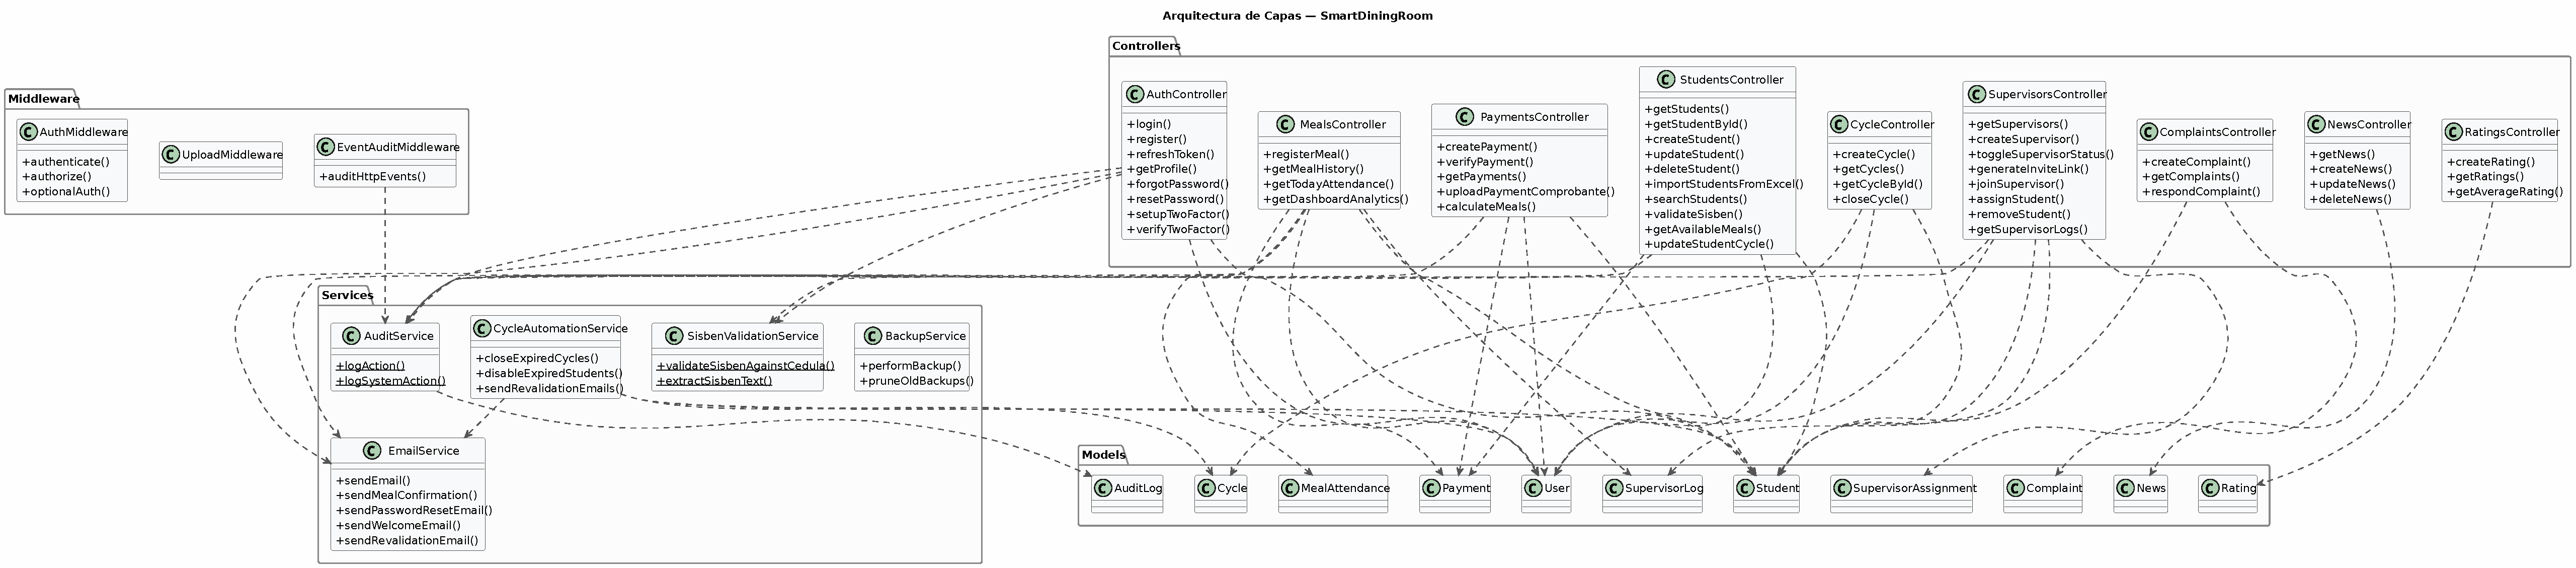
\includegraphics[width=\textwidth]{figs/architecture.pdf}
\caption{Arquitectura general del sistema SmartComedor.}
\label{fig:arquitectura}
\end{figure}

\subsubsection{Stack tecnológico}
La Tabla~\ref{tab:stack} resume las tecnologías por capa.

\begin{table}[H]
\centering
\caption{Stack tecnológico}
\label{tab:stack}
\begin{tabularx}{\textwidth}{L{0.22\textwidth} X}
\toprule
\textbf{Capa / aspecto} & \textbf{Tecnología} \\
\midrule
Frontend & React 18 + TypeScript + Vite + Material UI (MUI) \\
Backend & Node.js + Express + TypeScript (API REST bajo \texttt{/api}) \\
Base de datos & PostgreSQL 14 con ORM Sequelize \\
Autenticación & JWT (access + refresh); contraseñas con bcrypt \\
Segundo factor & TOTP (speakeasy + qrcode) \\
Correo & Nodemailer (SMTP) \\
OCR / PDF & tesseract.js, pdf-parse \\
Archivos / importación & multer; xlsx \\
Programación de tareas & node-cron \\
Contenedores & Docker Compose (perfiles \texttt{dev} y \texttt{prod}, nginx en prod) \\
\bottomrule
\end{tabularx}
\end{table}

\subsubsection{Reglas de negocio principales}
\begin{itemize}[leftmargin=1.4em]
  \item \textbf{Precio del almuerzo:} \texttt{MEAL\_PRICE = 2000} (COP). Los almuerzos
  incluidos en un pago se calculan como $\lfloor monto/2000 \rfloor$; el residuo
  ($monto \bmod 2000$) no genera almuerzo.
  \item \textbf{Monto mínimo de recarga:} un pago debe ser $\geq 2000$; en caso
  contrario se rechaza con HTTP 400.
  \item \textbf{Almuerzos disponibles:} se calculan sobre los pagos \emph{verificados}
  como $\sum (mealsIncluded - mealsUsed)$.
  \item \textbf{Un almuerzo por día:} un estudiante no puede registrar dos almuerzos el
  mismo día.
  \item \textbf{Días autorizados:} el almuerzo solo se registra en los días del comedor
  asignados al estudiante (\texttt{diasComedor}).
  \item \textbf{Elegibilidad SISBÉN:} las categorías válidas pertenecen a los grupos A,
  B y C; la validación coteja cédula, nombre y apellido contra la cédula frontal.
  \item \textbf{Autorización de cuentas:} un usuario con \texttt{isAuthorized = false}
  no puede iniciar sesión.
  \item \textbf{Invitación de supervisores:} el enlace de invitación es válido por 48
  horas.
  \item \textbf{Ciclos:} un ciclo vencido (\texttt{endDate} $<$ hoy) con estado
  \texttt{Activo} se cierra automáticamente.
\end{itemize}

% ────────────────────────────────────────────────────────────────────────────
\section{Modelo de requerimientos}

\subsection{Descripción}
El modelo de requerimientos especifica qué debe hacer el sistema (requisitos funcionales,
RF) y bajo qué condiciones de calidad (requisitos no funcionales, RNF)
\parencite{sommerville2011}. Los requisitos se derivaron del análisis del problema, de
las rutas REST implementadas, de los controladores y de las reglas de negocio
verificadas por las pruebas. Se emplea la convención RF-XX y RNF-XX, con prioridad Alta,
Media o Baja.

\subsection{Requisitos funcionales}

\begin{longtable}{c L{0.62\textwidth} c}
\caption{Requisitos funcionales del sistema}\label{tab:rf}\\
\toprule
\textbf{ID} & \textbf{Requisito} & \textbf{Prioridad} \\
\midrule
\endfirsthead
\multicolumn{3}{c}{\tablename\ \thetable\ -- \textit{continuación}}\\
\toprule
\textbf{ID} & \textbf{Requisito} & \textbf{Prioridad} \\
\midrule
\endhead
\midrule \multicolumn{3}{r}{\textit{continúa en la siguiente página}}\\
\endfoot
\bottomrule
\endlastfoot
RF-01 & Registro de estudiante con datos personales/académicos y carga de archivos (SISBÉN, cédula frontal, horario PDF, recibo de pago). & Alta \\
RF-02 & Iniciar sesión con email, contraseña y rol, retornando access token y refresh token JWT. & Alta \\
RF-03 & Rechazar el inicio de sesión ante campos faltantes (400), credenciales inválidas (401), usuario inactivo (401), rol no coincidente (403) o cuenta no autorizada (403). & Alta \\
RF-04 & Refrescar el access token a partir de un refresh token válido. & Alta \\
RF-05 & Consultar y actualizar el perfil del usuario autenticado. & Media \\
RF-06 & Cambiar la contraseña validando la contraseña actual. & Media \\
RF-07 & Recuperar la contraseña por correo con token, sin revelar si el email existe. & Alta \\
RF-08 & Restablecer la contraseña con un token válido y no expirado. & Alta \\
RF-09 & Configurar y verificar 2FA (TOTP) exclusivamente para estudiantes. & Media \\
RF-10 & Listar estudiantes con paginación y búsqueda. & Alta \\
RF-11 & Consultar un estudiante por ID, incluyendo sus almuerzos disponibles. & Alta \\
RF-12 & Crear un estudiante y su usuario asociado. & Alta \\
RF-13 & Actualizar y deshabilitar (soft delete) un estudiante. & Alta \\
RF-14 & Importar estudiantes masivamente desde Excel (.xlsx). & Alta \\
RF-15 & Buscar estudiantes (por cédula y otros filtros) para el registro de almuerzo. & Alta \\
RF-16 & Calcular los almuerzos disponibles a partir de los pagos verificados. & Alta \\
RF-17 & Validar el SISBÉN cotejando cédula, nombre y apellido contra la cédula frontal. & Alta \\
RF-18 & Actualizar el ciclo de un estudiante (revalidación/deshabilitación). & Media \\
RF-19 & Listar supervisores y sus bitácoras. & Media \\
RF-20 & Crear un supervisor con contraseña temporal. & Alta \\
RF-21 & Actualizar, deshabilitar y cambiar el estado (activo/autorizado) de un supervisor. & Media \\
RF-22 & Generar un enlace de invitación válido por 48 h para autorregistro de supervisor. & Media \\
RF-23 & Unirse mediante invitación validando el token. & Media \\
RF-24 & Asignar y remover estudiantes a un supervisor, evitando duplicados. & Media \\
RF-25 & Consultar los estudiantes asignados a un supervisor. & Media \\
RF-26 & Crear un pago asociado a un estudiante, calculando los almuerzos incluidos. & Alta \\
RF-27 & Cargar los comprobantes del pago (comprobante, recibo universidad, recibo banco). & Alta \\
RF-28 & Calcular los almuerzos de un monto, rechazando montos $<$ \$2000. & Alta \\
RF-29 & Listar pagos con paginación y filtros (por estudiante y por estado). & Alta \\
RF-30 & Verificar un pago (marcar \texttt{isVerified}, registrar \texttt{verifiedBy} y \texttt{verifiedAt}). & Alta \\
RF-31 & Registrar el almuerzo validando estudiante activo, día autorizado, no haber comido hoy y disponibilidad. & Alta \\
RF-32 & Decrementar la disponibilidad y registrar un \texttt{SupervisorLog} al registrar el almuerzo. & Alta \\
RF-33 & Consultar el historial de asistencia con filtros por estudiante y fechas. & Media \\
RF-34 & Consultar la asistencia del día. & Media \\
RF-35 & Ofrecer analítica del tablero (métricas agregadas). & Media \\
RF-36 & Crear, listar y consultar ciclos. & Media \\
RF-37 & Cerrar un ciclo manualmente. & Media \\
RF-38 & Cerrar automáticamente los ciclos vencidos y gestionar la revalidación. & Media \\
RF-39 & Calificar el servicio (1--5 estrellas + comentario opcional). & Media \\
RF-40 & Consultar calificaciones y su promedio/distribución. & Baja \\
RF-41 & Crear quejas, sugerencias o comentarios, de forma anónima o identificada. & Media \\
RF-42 & Responder y marcar como resueltas las quejas. & Media \\
RF-43 & Publicar, editar y eliminar (soft delete) noticias, y listarlas. & Baja \\
RF-44 & Registrar en auditoría las acciones y eventos HTTP sensibles. & Alta \\
RF-45 & Consultar y filtrar la auditoría (acción, método, código, ruta, rol, fechas) con paginación. & Alta \\
\end{longtable}

\subsection{Requisitos no funcionales}
Los RNF se organizan según el modelo de calidad ISO/IEC 25010 \parencite{iso25010}.

\begin{longtable}{c L{0.20\textwidth} L{0.58\textwidth}}
\caption{Requisitos no funcionales del sistema}\label{tab:rnf}\\
\toprule
\textbf{ID} & \textbf{Categoría} & \textbf{Requisito} \\
\midrule
\endfirsthead
\multicolumn{3}{c}{\tablename\ \thetable\ -- \textit{continuación}}\\
\toprule
\textbf{ID} & \textbf{Categoría} & \textbf{Requisito} \\
\midrule
\endhead
\bottomrule
\endlastfoot
RNF-01 & Seguridad & Contraseñas almacenadas cifradas con bcrypt (hash + salt). \\
RNF-02 & Seguridad & Control de acceso por JWT (access 15 min, refresh 7 días) y autorización por rol. \\
RNF-03 & Seguridad & Rechazo de peticiones sin token (401) y de rol no permitido (403). \\
RNF-04 & Seguridad & No filtrar trazas de error (stack traces); mensajes genéricos. \\
RNF-05 & Seguridad & Recuperación de contraseña sin revelar si un correo existe. \\
RNF-06 & Seguridad & Cabeceras de seguridad (nosniff, anti-clickjacking) y sin \texttt{X-Powered-By}. \\
RNF-07 & Seguridad & Validación de filtros de auditoría contra listas blancas. \\
RNF-08 & Seguridad & 2FA (TOTP) como segundo factor para estudiantes. \\
RNF-09 & Rendimiento & Consultas críticas y autenticación responden en menos de 3 s. \\
RNF-10 & Rendimiento & Soportar pruebas de carga/estrés (p. ej. 200 hilos) con umbral configurable. \\
RNF-11 & Rendimiento & Listados paginados para acotar el volumen por respuesta. \\
RNF-12 & Disponibilidad & Healthcheck de PostgreSQL y perfiles dev/prod. \\
RNF-13 & Disponibilidad & Endpoint de salud \texttt{GET /api/health}. \\
RNF-14 & Disponibilidad & Backups diarios (\texttt{pg\_dump}) con retención de 30 días. \\
RNF-15 & Disponibilidad & Cierre de ciclos y revalidación automáticos y programados. \\
RNF-16 & Usabilidad & UI con componentes MUI responsive, labels, estados y mensajes guiados. \\
RNF-17 & Usabilidad & Experiencia diferenciada por rol. \\
RNF-18 & Usabilidad & Formularios con label/aria-label y landmark \texttt{main}. \\
RNF-19 & Portabilidad & Funcionar en Chrome, Firefox, Edge y Safari (escritorio). \\
RNF-20 & Portabilidad & Desplegable en cualquier entorno con Docker. \\
RNF-21 & Portabilidad & Operar con APIs estándar del navegador sin polyfills. \\
RNF-22 & Mantenibilidad & Código en TypeScript (tipado estático) en cliente y servidor. \\
RNF-23 & Mantenibilidad & Auditoría de acciones sensibles y bitácora de supervisor. \\
RNF-24 & Mantenibilidad & Identificador legible (\texttt{uid}) por entidad con prefijo. \\
RNF-25 & Mantenibilidad & Batería de pruebas automatizadas y reportes de cobertura. \\
\end{longtable}

% ────────────────────────────────────────────────────────────────────────────
\section{Modelo de casos de uso}

\subsection{Diagramas de caso de uso}
La Figura~\ref{fig:casos} presenta el diagrama general de casos de uso. La
Tabla~\ref{tab:catalogo} lista el catálogo de casos de uso del sistema.

\begin{figure}[H]
\centering
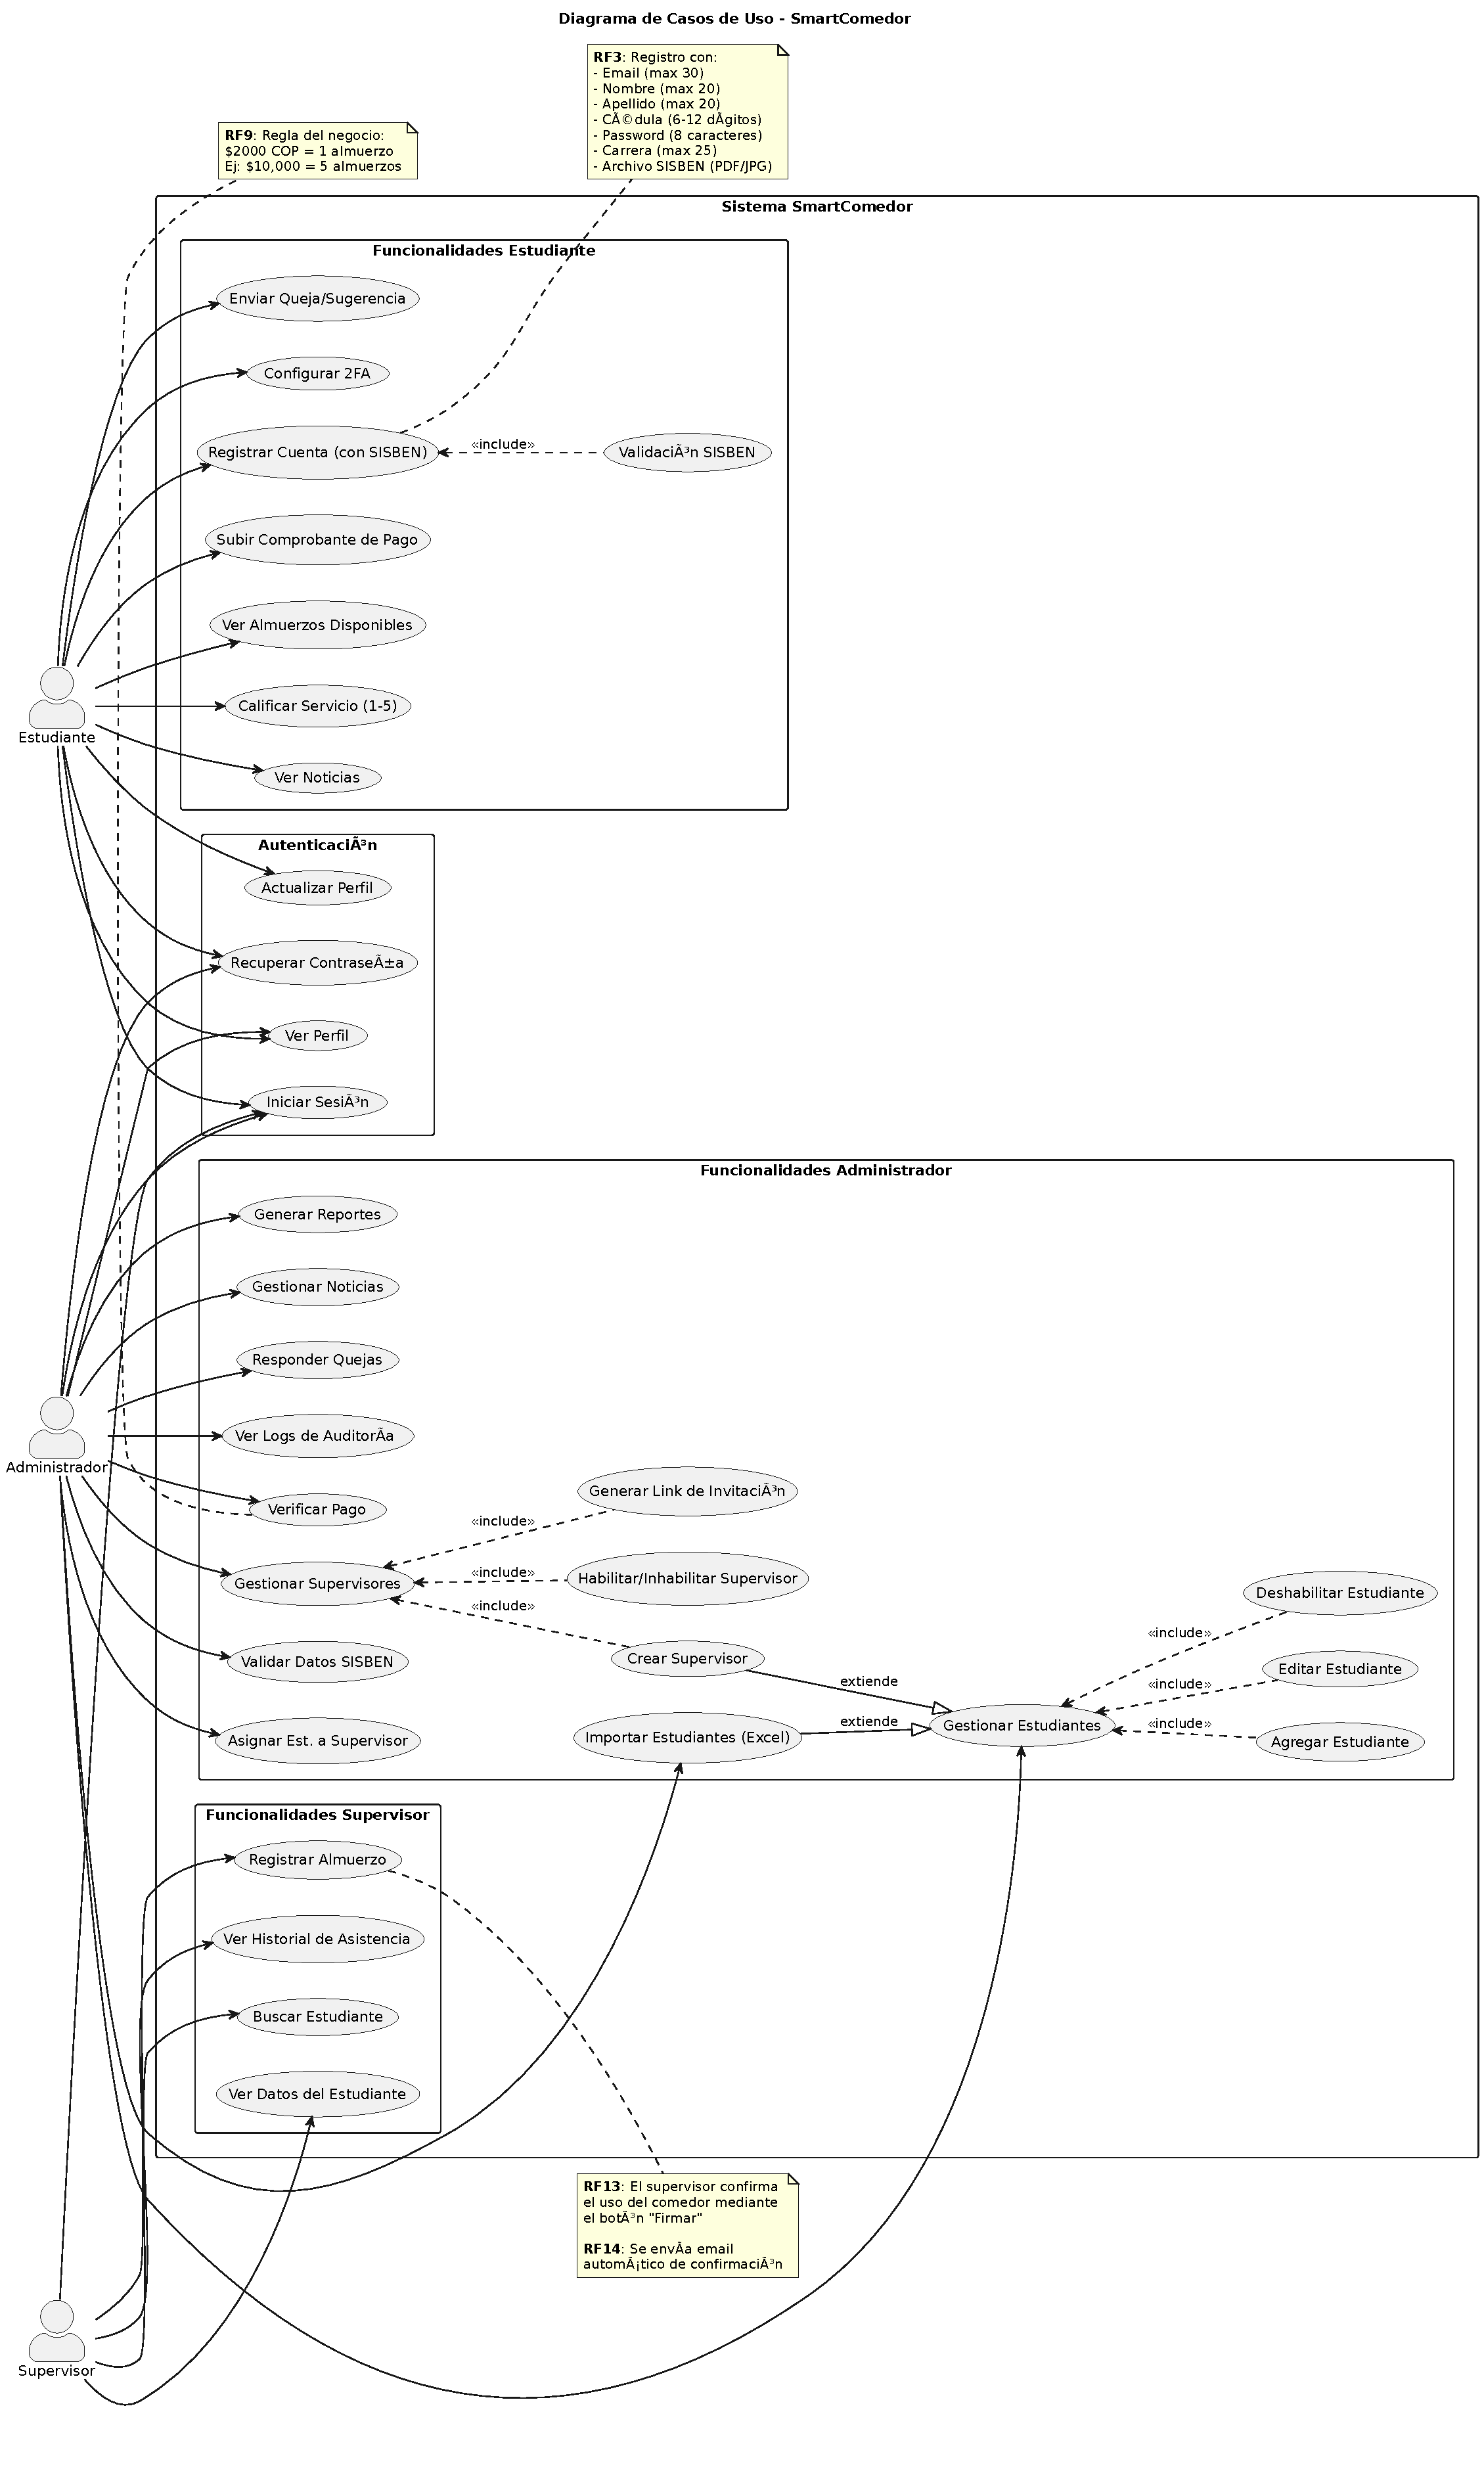
\includegraphics[width=\textwidth]{figs/use-cases.pdf}
\caption{Diagrama general de casos de uso.}
\label{fig:casos}
\end{figure}

\begin{longtable}{c L{0.55\textwidth} L{0.28\textwidth}}
\caption{Catálogo de casos de uso}\label{tab:catalogo}\\
\toprule
\textbf{ID} & \textbf{Caso de uso} & \textbf{Actor principal} \\
\midrule
\endfirsthead
\toprule
\textbf{ID} & \textbf{Caso de uso} & \textbf{Actor principal} \\
\midrule
\endhead
\bottomrule
\endlastfoot
CU-01 & Registrar estudiante & Estudiante \\
CU-02 & Iniciar sesión & Todos \\
CU-03 & Recuperar/restablecer contraseña & Todos \\
CU-04 & Configurar y verificar 2FA & Estudiante \\
CU-05 & Gestionar estudiantes (CRUD) & Administrador \\
CU-06 & Importar estudiantes desde Excel & Administrador \\
CU-07 & Validar SISBÉN & Administrador \\
CU-08 & Gestionar supervisores & Administrador \\
CU-09 & Invitar supervisor / unirse por invitación & Admin / Supervisor \\
CU-10 & Asignar estudiantes a supervisor & Administrador \\
CU-11 & Subir pago y comprobantes & Estudiante \\
CU-12 & Verificar pago & Administrador \\
CU-13 & Calcular almuerzos por monto & Autenticado \\
CU-14 & Registrar almuerzo & Supervisor \\
CU-15 & Consultar historial / asistencia del día & Autenticado \\
CU-16 & Consultar analítica del tablero & Admin / Auditor \\
CU-17 & Gestionar ciclos / cierre automático & Admin / Sistema \\
CU-18 & Calificar servicio & Estudiante \\
CU-19 & Enviar y responder quejas & Estudiante / Admin \\
CU-20 & Gestionar noticias & Administrador \\
CU-21 & Consultar auditoría & Admin / Auditor \\
\end{longtable}

\subsection{Descripción de casos de uso}
% Generado por gen_casos_uso.py

Esta seccion documenta los veintiun casos de uso del sistema con la plantilla extendida (objetivo, precondiciones, condiciones de exito y fracaso, actores y flujo de eventos). Cada caso se acompana de su diagrama de caso de uso, su diagrama de secuencia y su diagrama de actividades, derivados de los controladores reales y verificados por las pruebas de la Segunda Parte.


\subsection{CU-01 --- Registrar estudiante}

\noindent\textbf{Endpoint(s):} \texttt{POST /api/auth/register}\par\vspace{4pt}

\begin{table}[H]\centering\small
\caption{Ficha del caso de uso CU-01 --- Registrar estudiante}
\begin{tabularx}{\textwidth}{L{0.26\textwidth} X}
\toprule
\textbf{Campo} & \textbf{Descripcion} \\ \midrule
Objetivo del contexto & Permitir que un aspirante cree su cuenta de estudiante en SmartComedor adjuntando los documentos requeridos (SISBEN, cedula y horario), para acceder al servicio de comedor. \\ \midrule
Precondiciones & El correo electronico no debe estar registrado previamente. \\ \midrule
Condicion de exito & Se crea el usuario (rol estudiante) y su perfil de estudiante con SISBEN sin validar. \\ \midrule
Condicion de fracaso & El registro se rechaza por falta de documento SISBEN o por correo ya existente. \\ \midrule
Actores principales & Estudiante (no autenticado) \\ \midrule
Actores secundarios & Servicio de almacenamiento de archivos \\
\bottomrule\end{tabularx}\end{table}
\begin{table}[H]\centering\small
\caption{Flujo principal de CU-01}
\begin{tabularx}{\textwidth}{C{0.10\textwidth} X}
\toprule \textbf{Paso} & \textbf{Accion} \\ \midrule
1 & El estudiante diligencia el formulario con sus datos personales y academicos. \\
2 & Adjunta el documento SISBEN, la cedula frontal y el horario. \\
3 & El sistema valida la presencia del archivo SISBEN. \\
4 & El sistema verifica que el correo no exista. \\
5 & El sistema cifra la contrasena (bcrypt) y crea el usuario y el estudiante. \\
6 & El sistema responde 201 Created. \\
\bottomrule\end{tabularx}\end{table}
\begin{table}[H]\centering\small
\caption{Extensiones (flujos alternativos) de CU-01}
\begin{tabularx}{\textwidth}{C{0.10\textwidth} X}
\toprule \textbf{Paso} & \textbf{Accion} \\ \midrule
3.1 & Falta el archivo SISBEN $\rightarrow$ HTTP 400. \\
4.1 & Correo ya registrado $\rightarrow$ HTTP 400. \\
\bottomrule\end{tabularx}\end{table}
\begin{figure}[H]\centering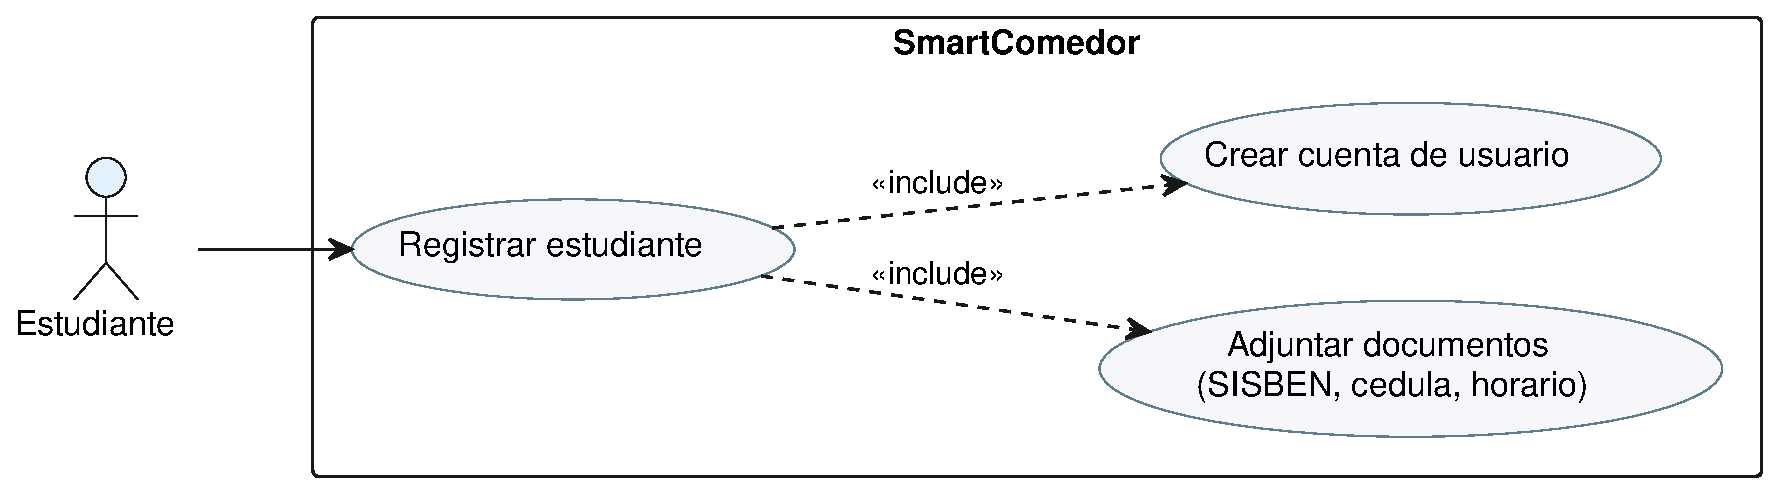
\includegraphics[width=\linewidth,height=0.30\textheight,keepaspectratio]{cu/cu01-uc.pdf}\caption{Diagrama de caso de uso --- CU-01}\end{figure}
\begin{figure}[H]\centering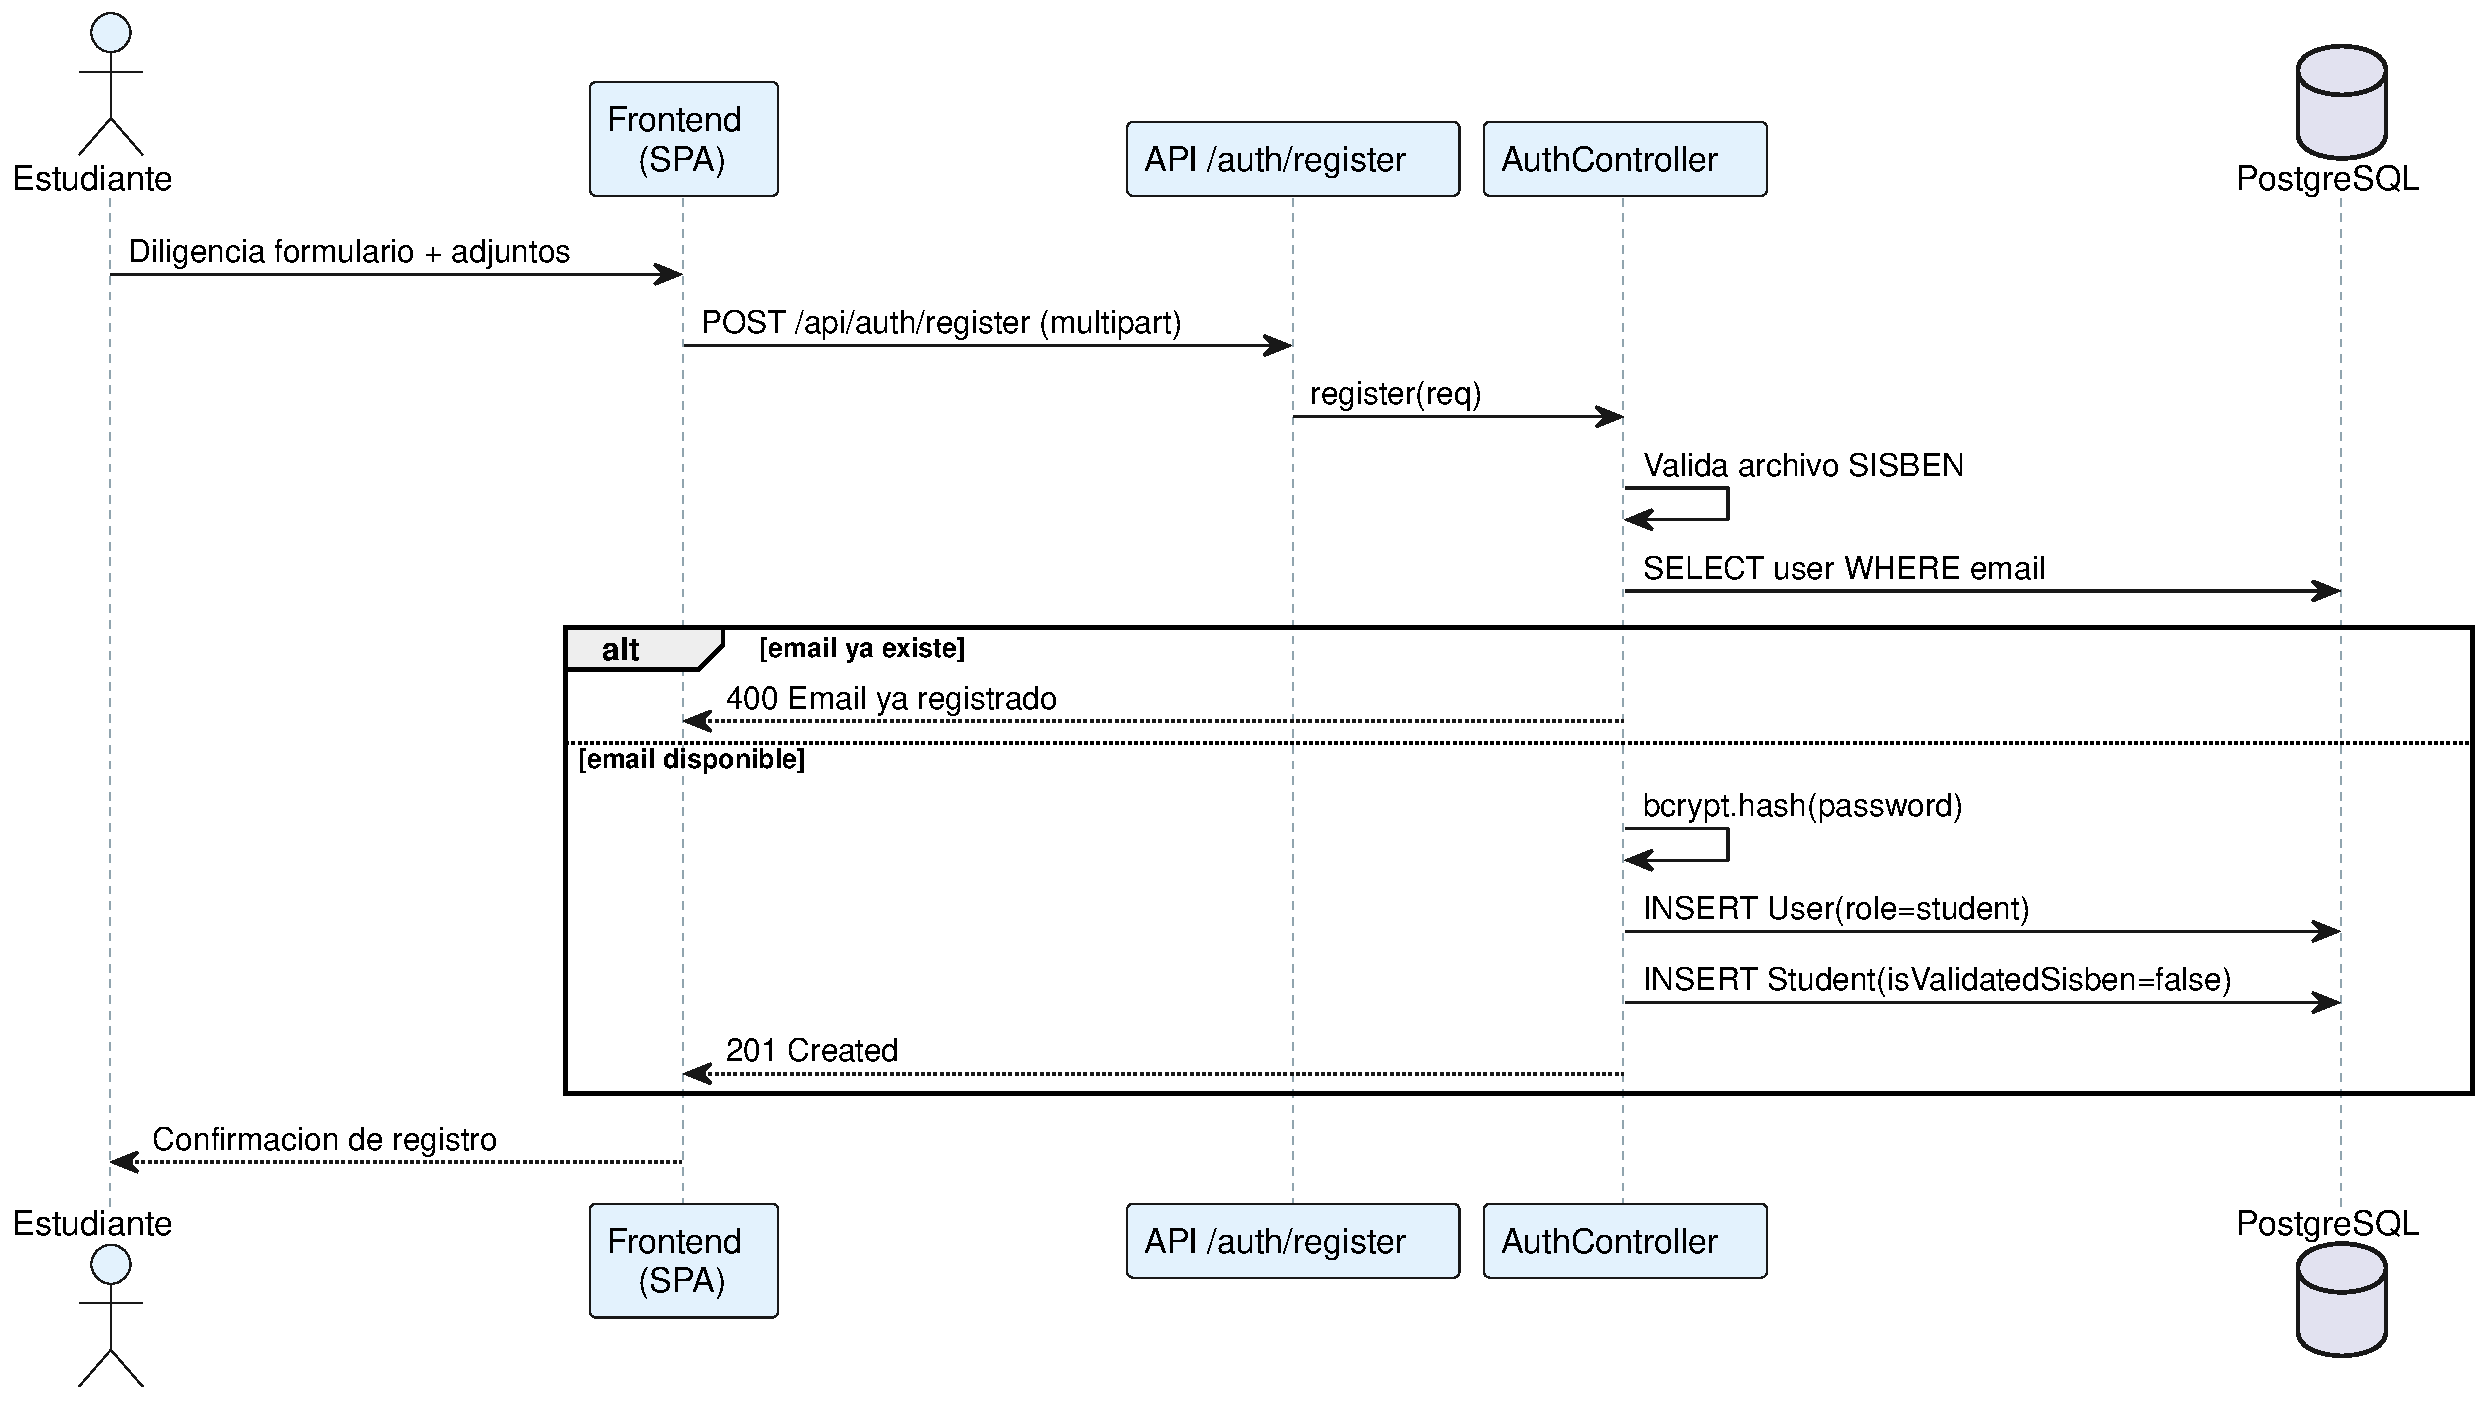
\includegraphics[width=\linewidth,height=0.42\textheight,keepaspectratio]{cu/cu01-seq.pdf}\caption{Diagrama de secuencia --- CU-01}\end{figure}
\begin{figure}[H]\centering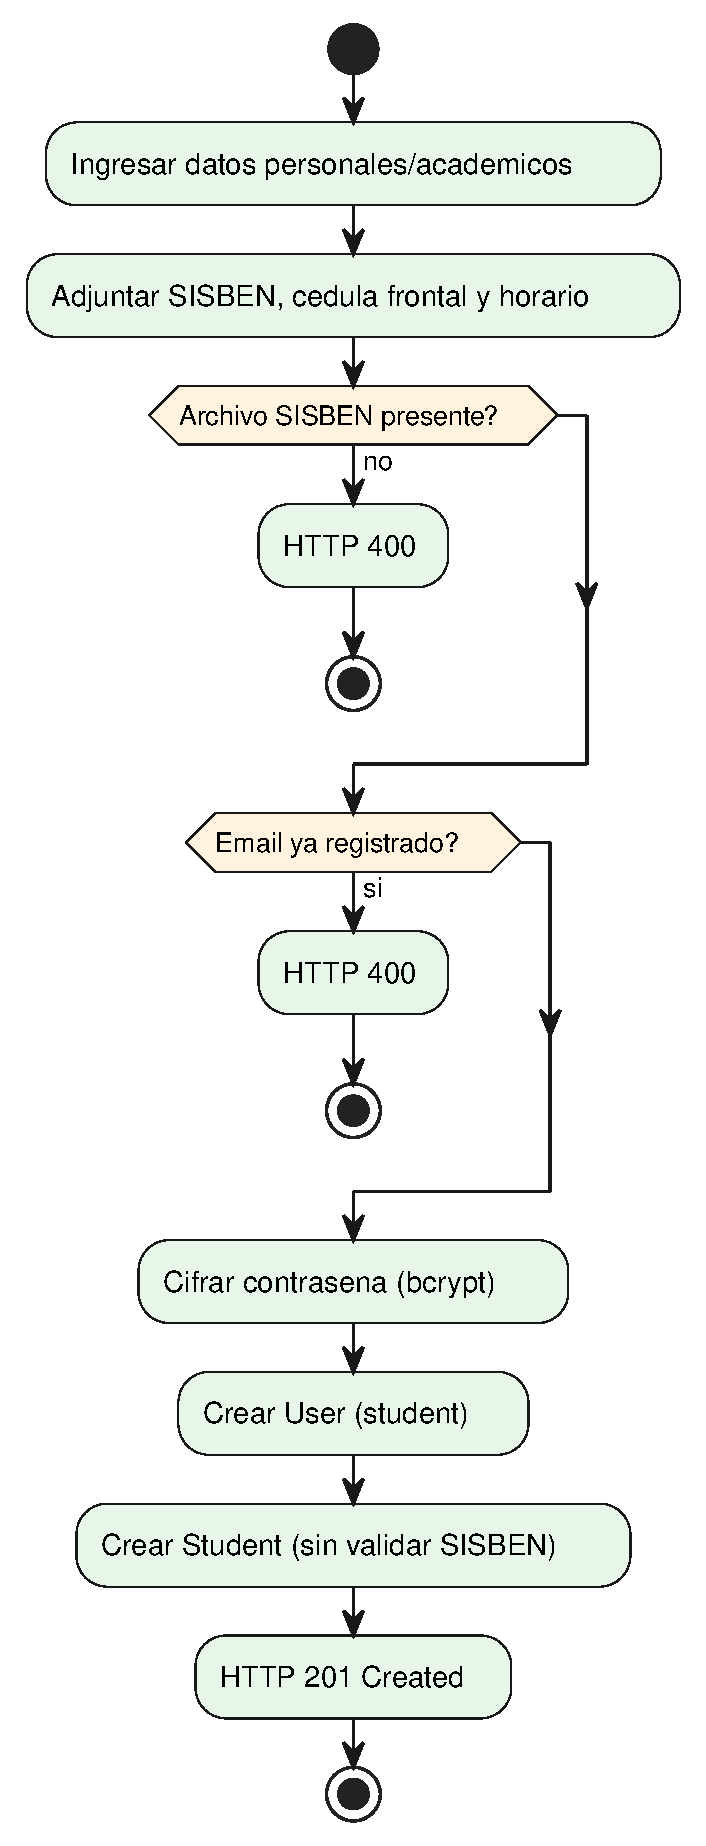
\includegraphics[width=\linewidth,height=0.46\textheight,keepaspectratio]{cu/cu01-act.pdf}\caption{Diagrama de actividades --- CU-01}\end{figure}

\subsection{CU-02 --- Iniciar sesion}

\noindent\textbf{Endpoint(s):} \texttt{POST /api/auth/login}\par\vspace{4pt}

\begin{table}[H]\centering\small
\caption{Ficha del caso de uso CU-02 --- Iniciar sesion}
\begin{tabularx}{\textwidth}{L{0.26\textwidth} X}
\toprule
\textbf{Campo} & \textbf{Descripcion} \\ \midrule
Objetivo del contexto & Permitir a un usuario autenticarse en el sistema mediante correo, contrasena y rol, obteniendo los tokens de acceso. \\ \midrule
Precondiciones & El usuario debe estar registrado y su cuenta activa. \\ \midrule
Condicion de exito & Se emiten los tokens de acceso y refresco; el usuario accede segun su rol. \\ \midrule
Condicion de fracaso & Acceso denegado por credenciales, estado o rol invalidos. \\ \midrule
Actores principales & Usuario (estudiante, supervisor, administrador, auditor) \\ \midrule
Actores secundarios & Servicio de autenticacion JWT \\
\bottomrule\end{tabularx}\end{table}
\begin{table}[H]\centering\small
\caption{Flujo principal de CU-02}
\begin{tabularx}{\textwidth}{C{0.10\textwidth} X}
\toprule \textbf{Paso} & \textbf{Accion} \\ \midrule
1 & El usuario ingresa correo, contrasena y rol. \\
2 & El sistema valida que los campos esten completos. \\
3 & El sistema busca al usuario por correo. \\
4 & El sistema verifica la contrasena con bcrypt.compare. \\
5 & El sistema valida que la cuenta este activa, autorizada y que el rol coincida. \\
6 & El sistema emite access y refresh token y responde 200. \\
\bottomrule\end{tabularx}\end{table}
\begin{table}[H]\centering\small
\caption{Extensiones (flujos alternativos) de CU-02}
\begin{tabularx}{\textwidth}{C{0.10\textwidth} X}
\toprule \textbf{Paso} & \textbf{Accion} \\ \midrule
2.1 & Campos faltantes $\rightarrow$ HTTP 400. \\
3.1 & Usuario inexistente $\rightarrow$ HTTP 401. \\
4.1 & Contrasena incorrecta $\rightarrow$ HTTP 401. \\
5.1 & Cuenta inactiva $\rightarrow$ 401; rol no coincide o no autorizado $\rightarrow$ 403. \\
\bottomrule\end{tabularx}\end{table}
\begin{figure}[H]\centering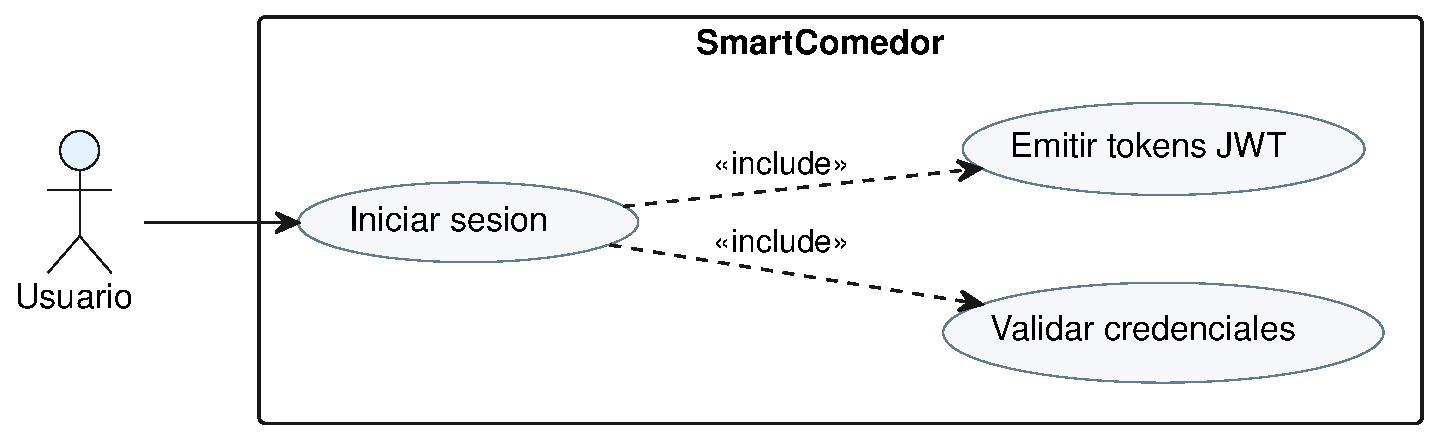
\includegraphics[width=\linewidth,height=0.30\textheight,keepaspectratio]{cu/cu02-uc.pdf}\caption{Diagrama de caso de uso --- CU-02}\end{figure}
\begin{figure}[H]\centering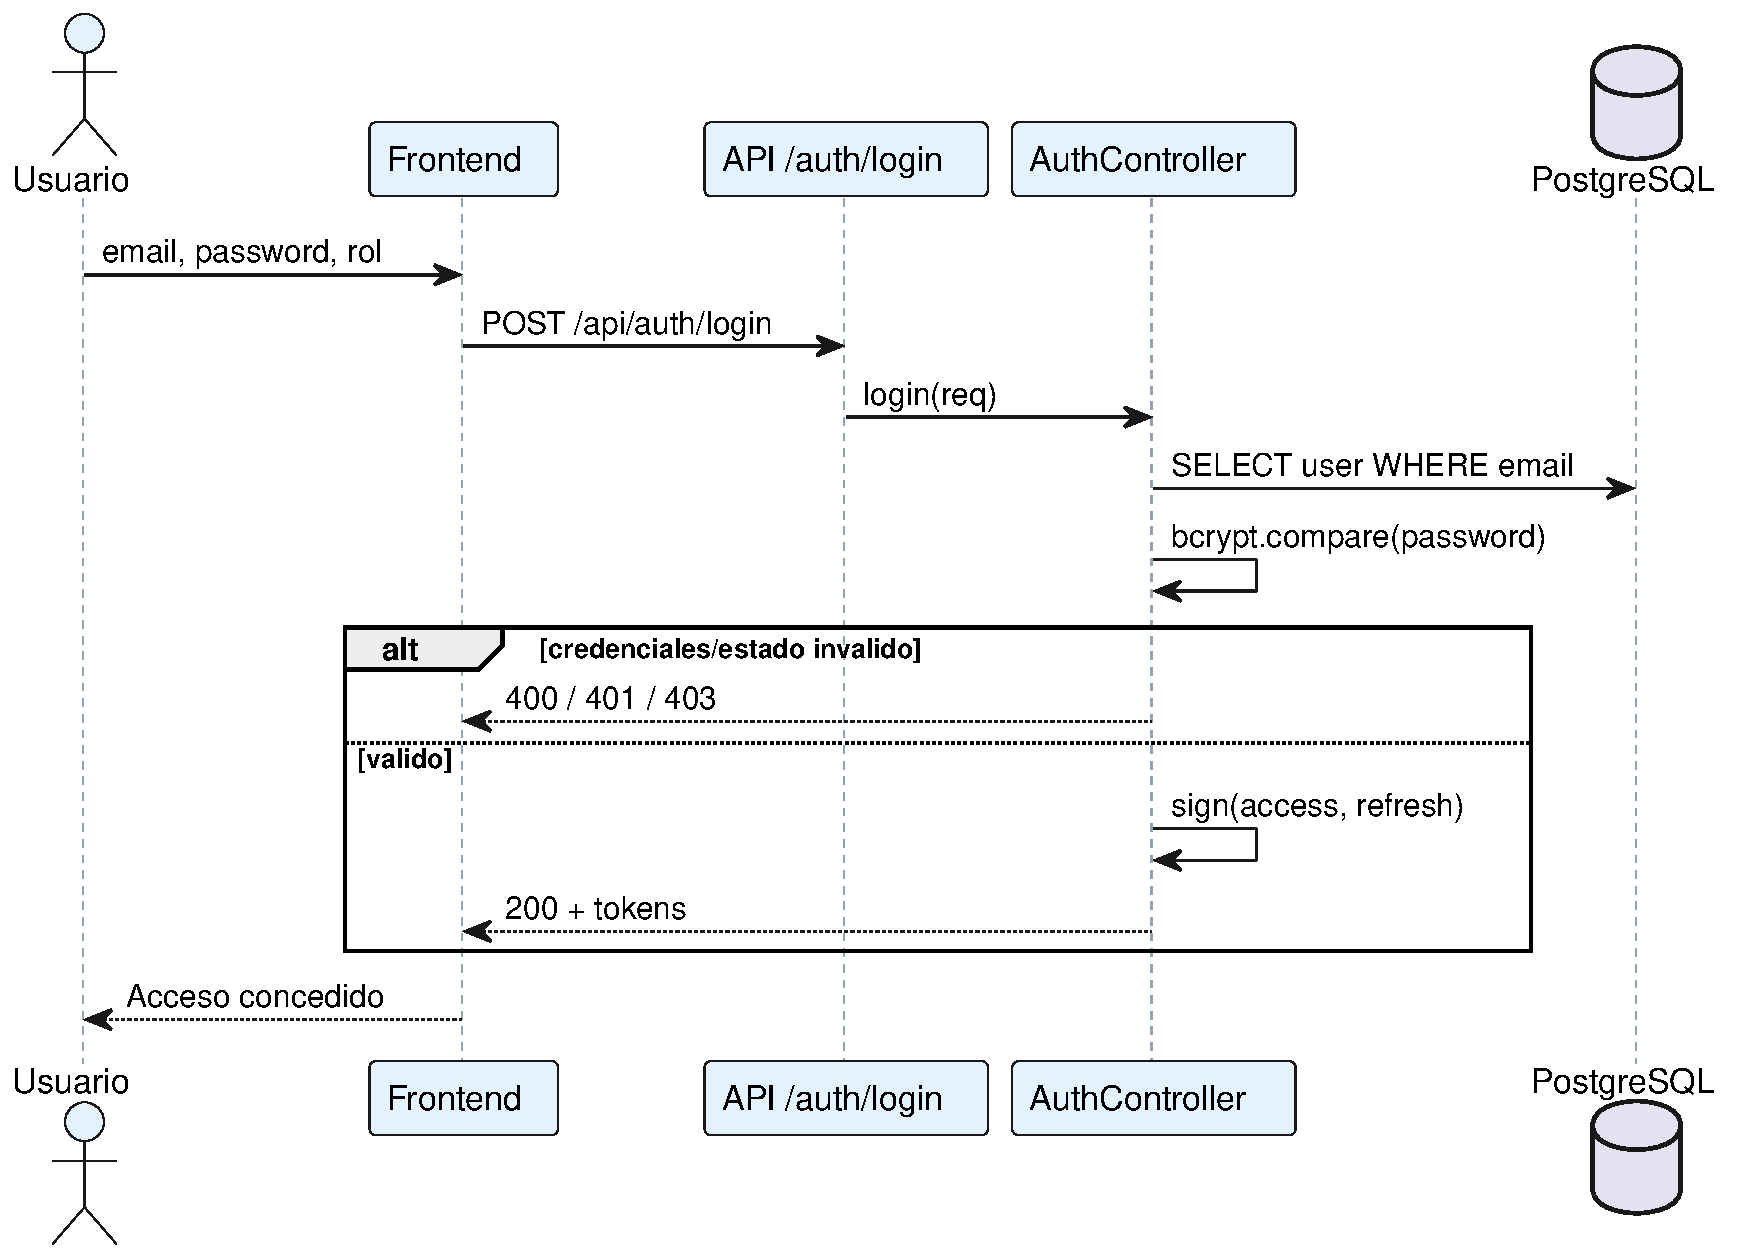
\includegraphics[width=\linewidth,height=0.42\textheight,keepaspectratio]{cu/cu02-seq.pdf}\caption{Diagrama de secuencia --- CU-02}\end{figure}
\begin{figure}[H]\centering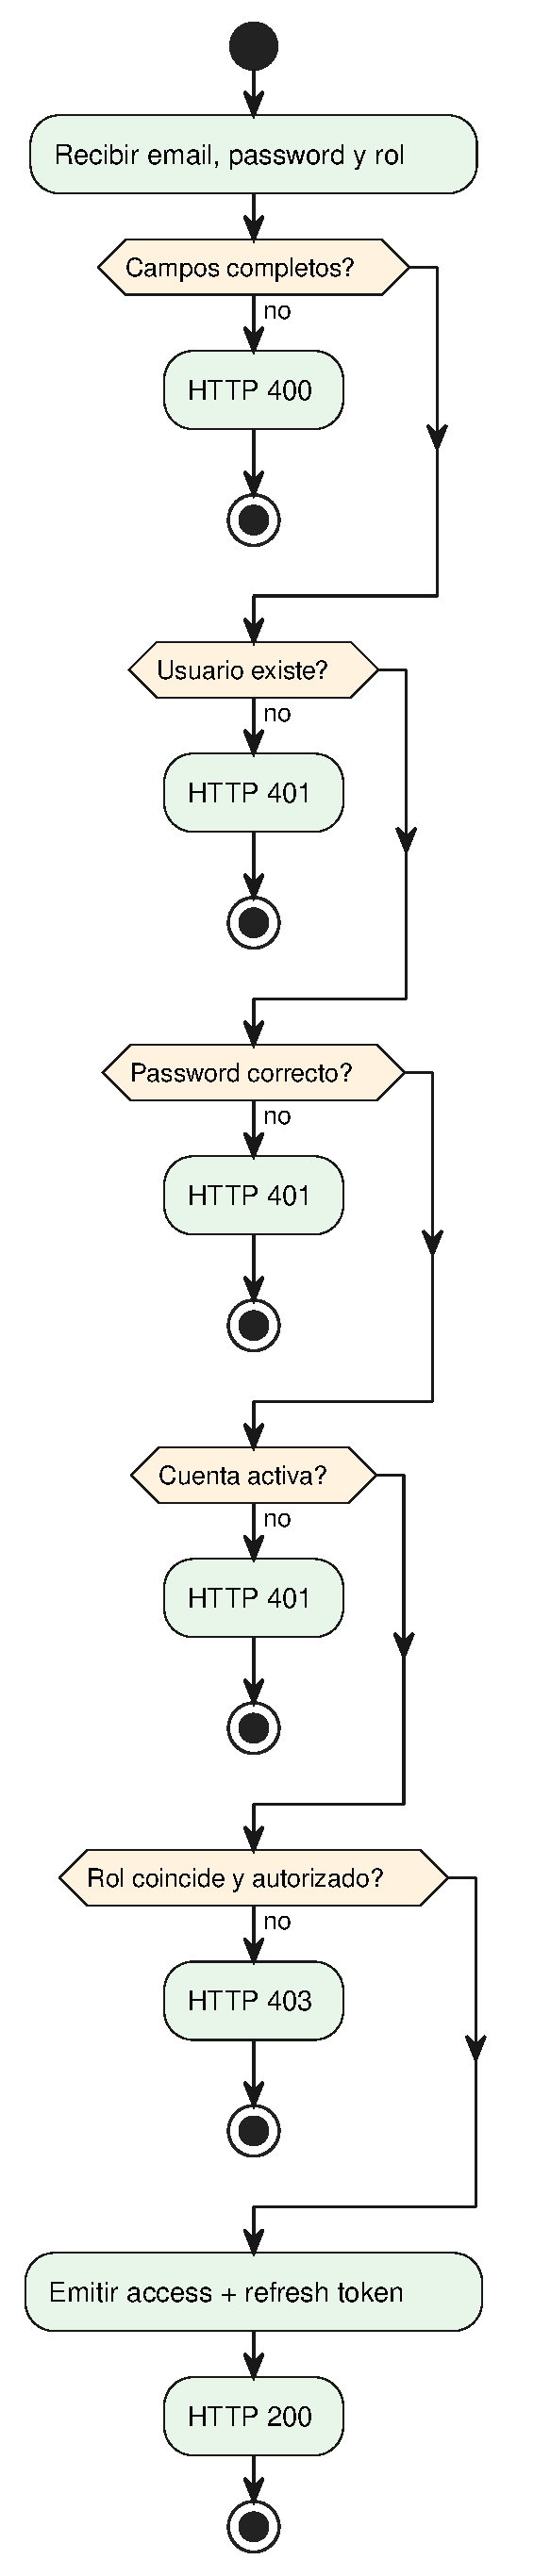
\includegraphics[width=\linewidth,height=0.46\textheight,keepaspectratio]{cu/cu02-act.pdf}\caption{Diagrama de actividades --- CU-02}\end{figure}

\subsection{CU-03 --- Recuperar y restablecer contrasena}

\noindent\textbf{Endpoint(s):} \texttt{POST /api/auth/forgot-password, POST /api/auth/reset-password}\par\vspace{4pt}

\begin{table}[H]\centering\small
\caption{Ficha del caso de uso CU-03 --- Recuperar y restablecer contrasena}
\begin{tabularx}{\textwidth}{L{0.26\textwidth} X}
\toprule
\textbf{Campo} & \textbf{Descripcion} \\ \midrule
Objetivo del contexto & Permitir al usuario recuperar el acceso cuando olvida su contrasena, mediante un enlace con token enviado por correo. \\ \midrule
Precondiciones & El usuario debe tener un correo registrado. \\ \midrule
Condicion de exito & La contrasena se actualiza y el usuario puede iniciar sesion. \\ \midrule
Condicion de fracaso & El token es invalido o esta expirado. \\ \midrule
Actores principales & Usuario \\ \midrule
Actores secundarios & Servicio de correo (Nodemailer) \\
\bottomrule\end{tabularx}\end{table}
\begin{table}[H]\centering\small
\caption{Flujo principal de CU-03}
\begin{tabularx}{\textwidth}{C{0.10\textwidth} X}
\toprule \textbf{Paso} & \textbf{Accion} \\ \midrule
1 & El usuario solicita recuperacion indicando su correo. \\
2 & El sistema genera un token con expiracion y lo almacena. \\
3 & El sistema envia un correo con el enlace (mensaje generico). \\
4 & El usuario abre el enlace e ingresa la nueva contrasena. \\
5 & El sistema valida el token y actualiza la contrasena cifrada. \\
6 & El sistema responde 200. \\
\bottomrule\end{tabularx}\end{table}
\begin{table}[H]\centering\small
\caption{Extensiones (flujos alternativos) de CU-03}
\begin{tabularx}{\textwidth}{C{0.10\textwidth} X}
\toprule \textbf{Paso} & \textbf{Accion} \\ \midrule
3.1 & Por seguridad, el mensaje no revela si el correo existe. \\
5.1 & Token invalido o expirado $\rightarrow$ HTTP 400. \\
\bottomrule\end{tabularx}\end{table}
\begin{figure}[H]\centering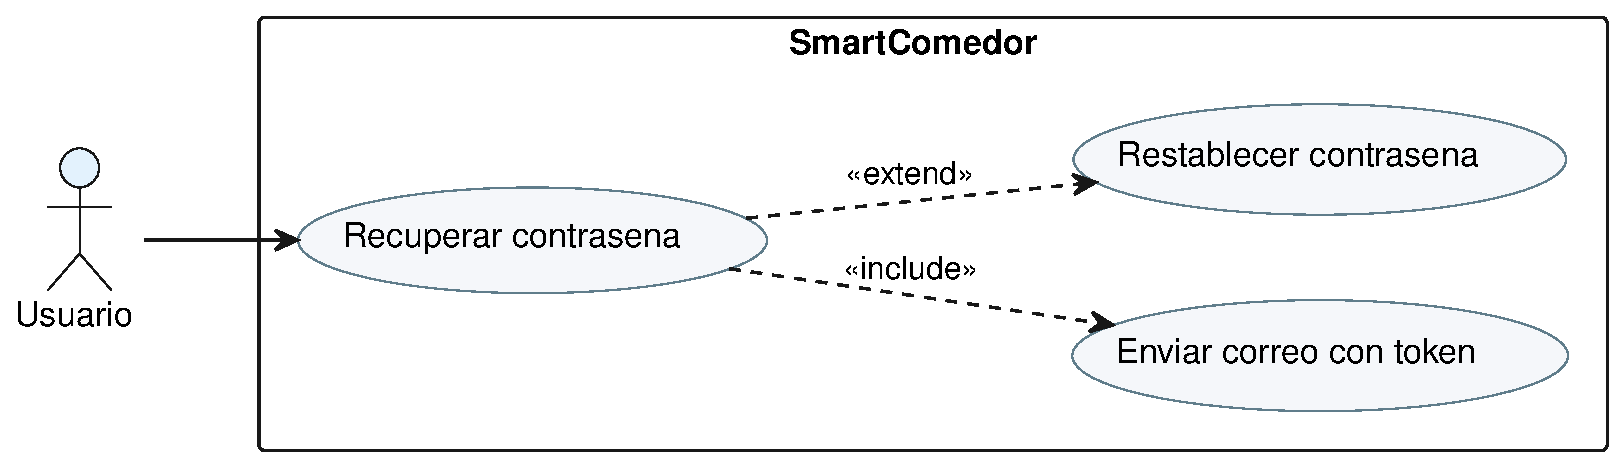
\includegraphics[width=\linewidth,height=0.30\textheight,keepaspectratio]{cu/cu03-uc.pdf}\caption{Diagrama de caso de uso --- CU-03}\end{figure}
\begin{figure}[H]\centering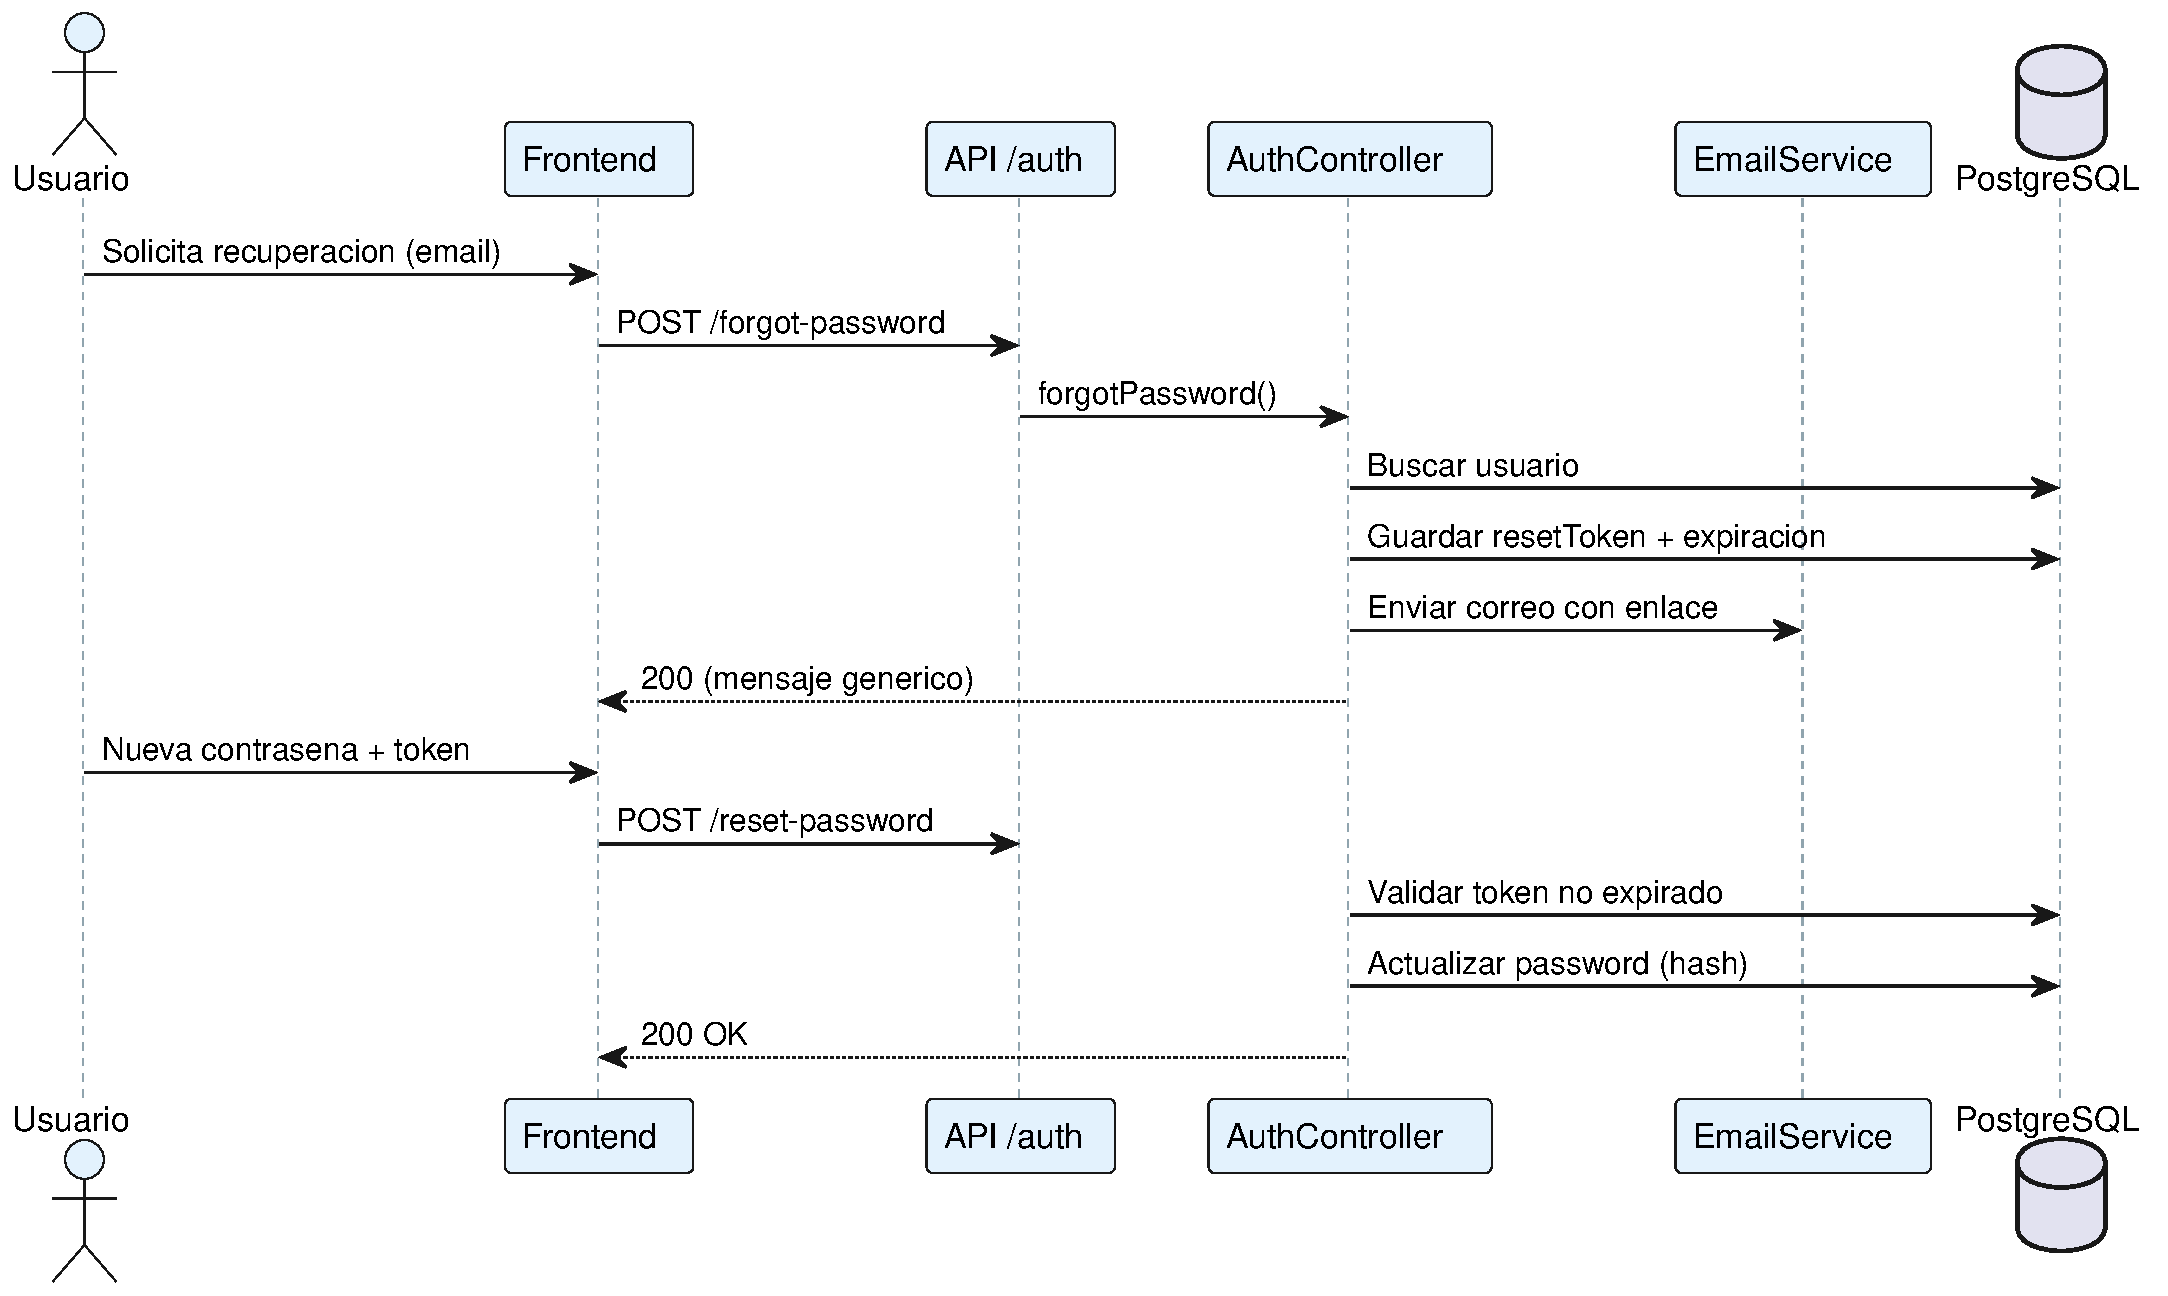
\includegraphics[width=\linewidth,height=0.42\textheight,keepaspectratio]{cu/cu03-seq.pdf}\caption{Diagrama de secuencia --- CU-03}\end{figure}
\begin{figure}[H]\centering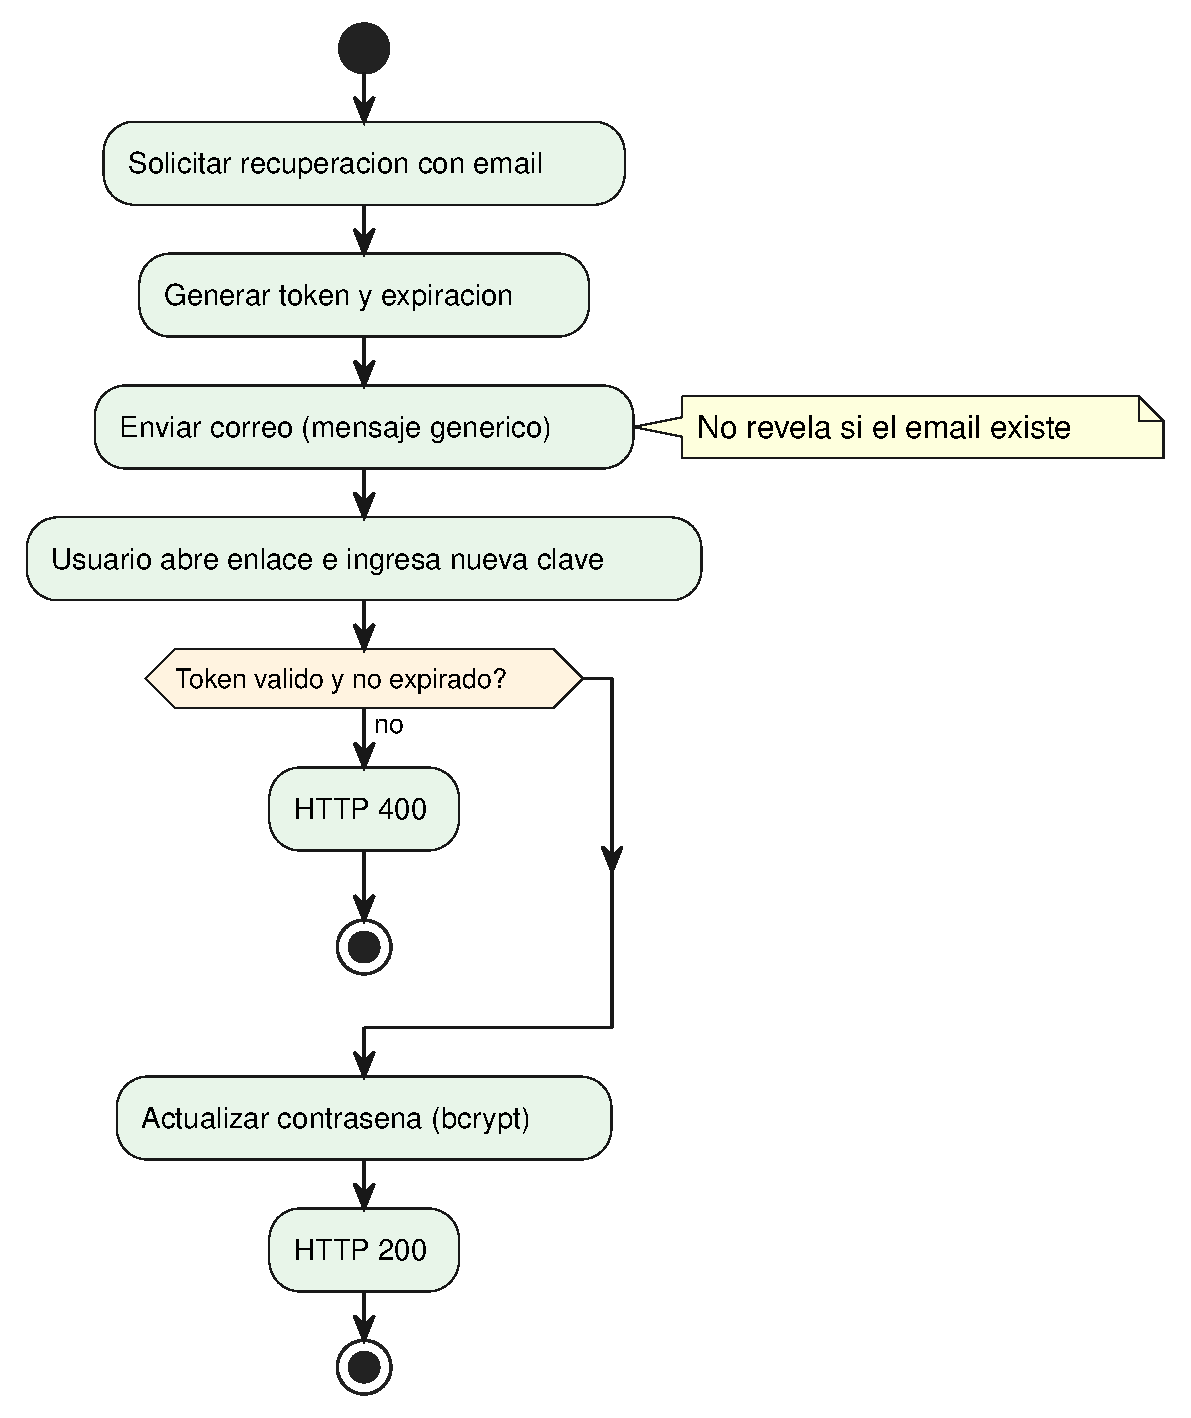
\includegraphics[width=\linewidth,height=0.46\textheight,keepaspectratio]{cu/cu03-act.pdf}\caption{Diagrama de actividades --- CU-03}\end{figure}

\subsection{CU-04 --- Configurar y verificar 2FA}

\noindent\textbf{Endpoint(s):} \texttt{POST /api/auth/setup-2fa, POST /api/auth/verify-2fa}\par\vspace{4pt}

\begin{table}[H]\centering\small
\caption{Ficha del caso de uso CU-04 --- Configurar y verificar 2FA}
\begin{tabularx}{\textwidth}{L{0.26\textwidth} X}
\toprule
\textbf{Campo} & \textbf{Descripcion} \\ \midrule
Objetivo del contexto & Permitir al estudiante activar un segundo factor de autenticacion (TOTP) para reforzar la seguridad de su cuenta. \\ \midrule
Precondiciones & El usuario debe estar autenticado. \\ \midrule
Condicion de exito & El segundo factor queda activo y se exige en posteriores inicios de sesion. \\ \midrule
Condicion de fracaso & El codigo TOTP ingresado es invalido. \\ \midrule
Actores principales & Estudiante \\ \midrule
Actores secundarios & Aplicacion autenticadora (TOTP) \\
\bottomrule\end{tabularx}\end{table}
\begin{table}[H]\centering\small
\caption{Flujo principal de CU-04}
\begin{tabularx}{\textwidth}{C{0.10\textwidth} X}
\toprule \textbf{Paso} & \textbf{Accion} \\ \midrule
1 & El usuario solicita activar 2FA. \\
2 & El sistema genera un secreto TOTP y un codigo QR. \\
3 & El usuario escanea el QR en su aplicacion autenticadora. \\
4 & El usuario ingresa el codigo de 6 digitos. \\
5 & El sistema verifica el codigo con speakeasy y activa el 2FA. \\
6 & El sistema responde 200. \\
\bottomrule\end{tabularx}\end{table}
\begin{table}[H]\centering\small
\caption{Extensiones (flujos alternativos) de CU-04}
\begin{tabularx}{\textwidth}{C{0.10\textwidth} X}
\toprule \textbf{Paso} & \textbf{Accion} \\ \midrule
5.1 & Codigo TOTP invalido $\rightarrow$ HTTP 400. \\
\bottomrule\end{tabularx}\end{table}
\begin{figure}[H]\centering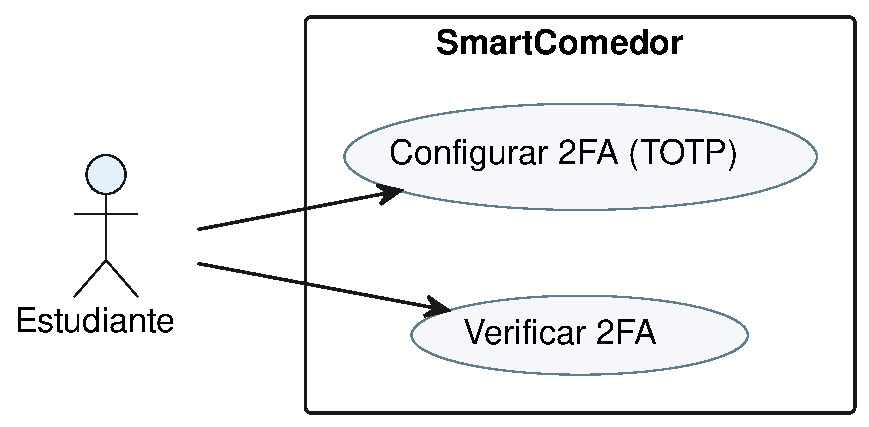
\includegraphics[width=\linewidth,height=0.30\textheight,keepaspectratio]{cu/cu04-uc.pdf}\caption{Diagrama de caso de uso --- CU-04}\end{figure}
\begin{figure}[H]\centering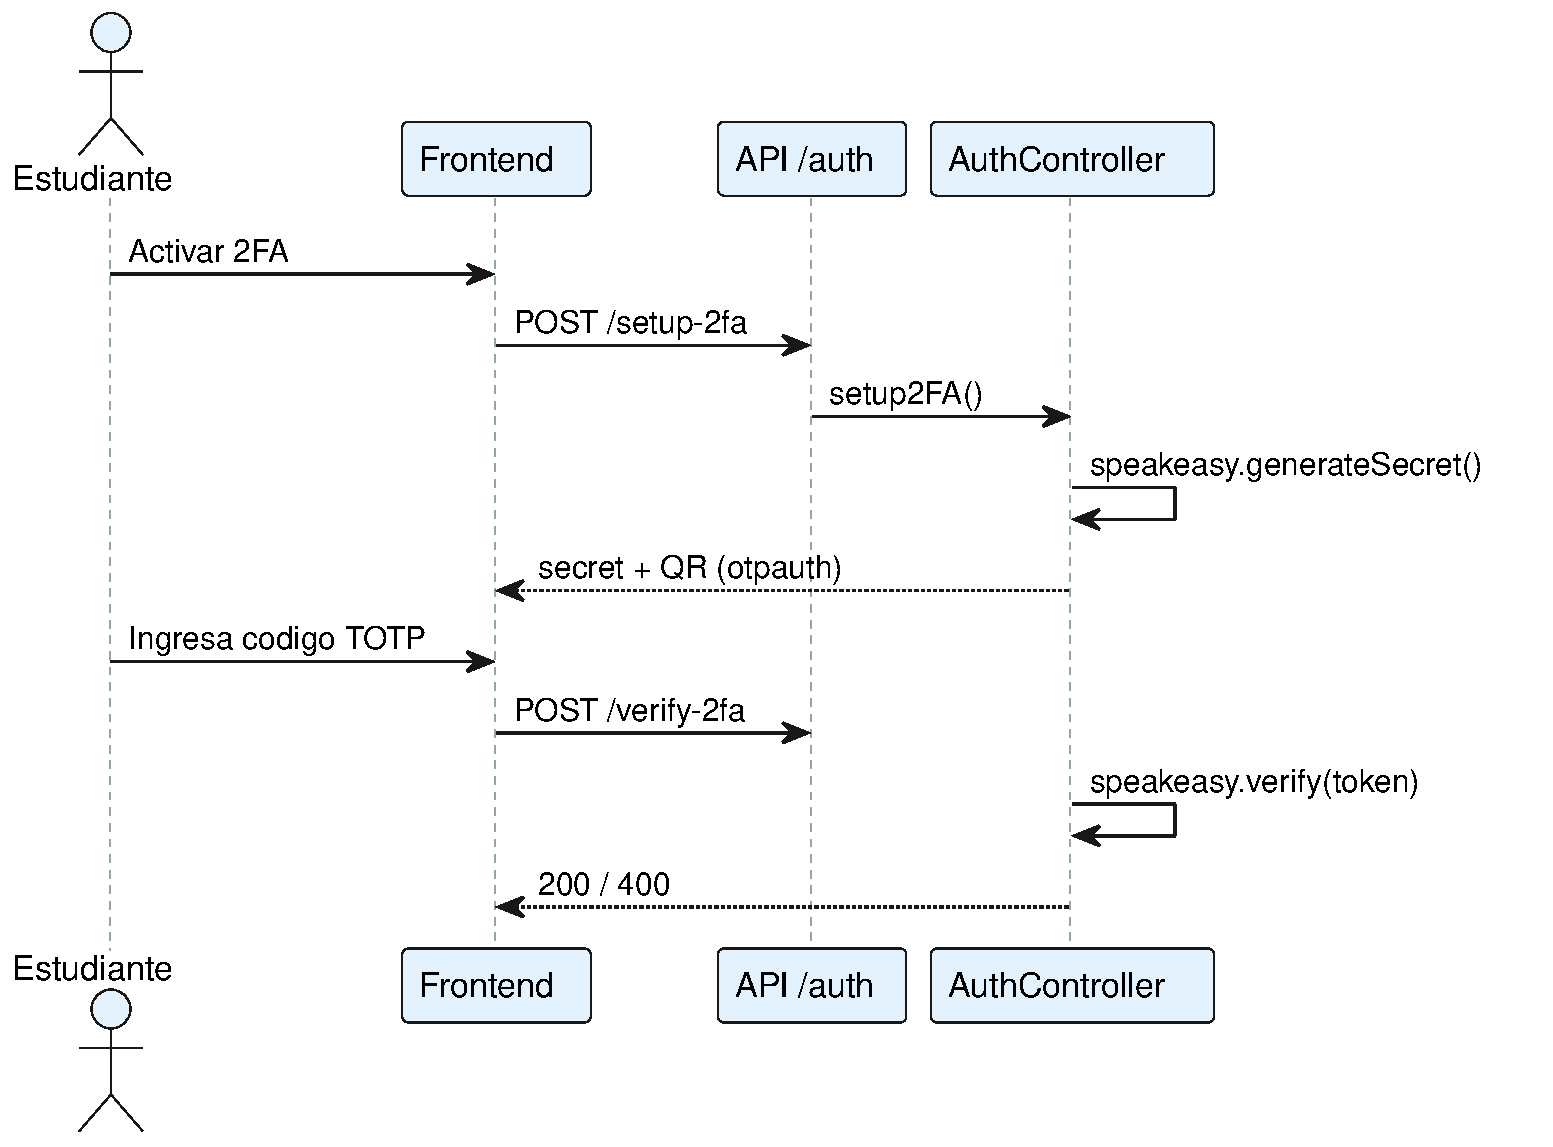
\includegraphics[width=\linewidth,height=0.42\textheight,keepaspectratio]{cu/cu04-seq.pdf}\caption{Diagrama de secuencia --- CU-04}\end{figure}
\begin{figure}[H]\centering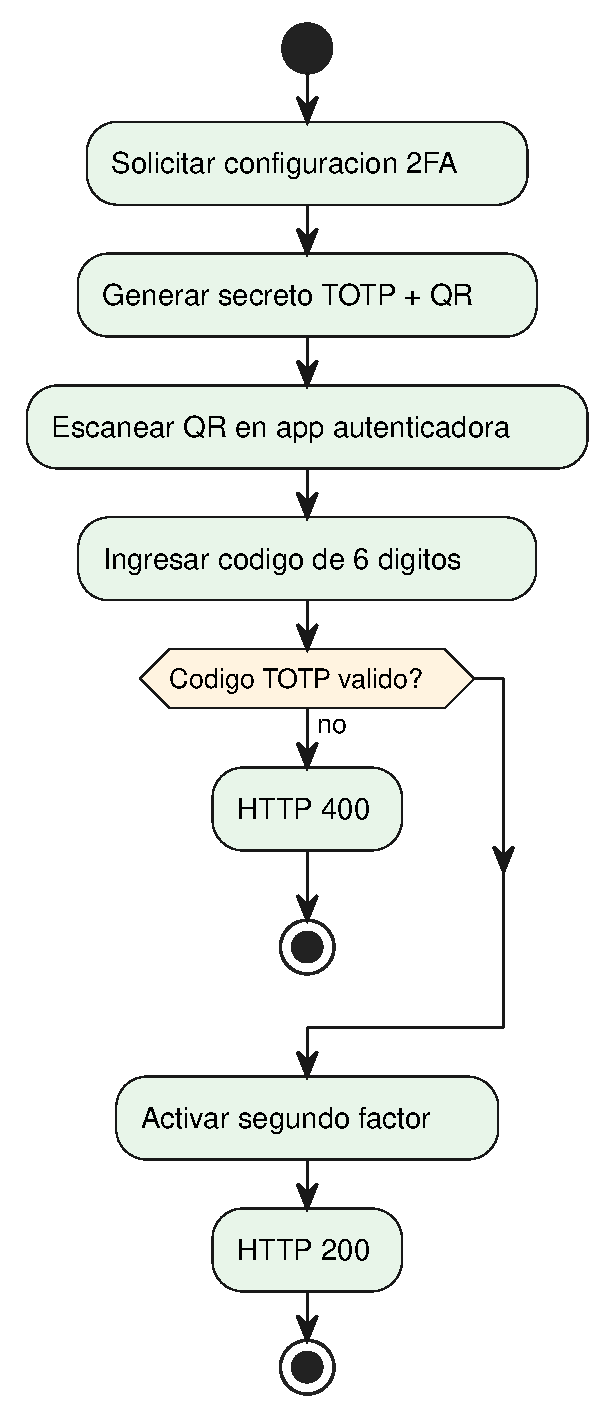
\includegraphics[width=\linewidth,height=0.46\textheight,keepaspectratio]{cu/cu04-act.pdf}\caption{Diagrama de actividades --- CU-04}\end{figure}

\subsection{CU-05 --- Gestionar estudiantes (CRUD)}

\noindent\textbf{Endpoint(s):} \texttt{GET/POST/PUT/DELETE /api/students}\par\vspace{4pt}

\begin{table}[H]\centering\small
\caption{Ficha del caso de uso CU-05 --- Gestionar estudiantes (CRUD)}
\begin{tabularx}{\textwidth}{L{0.26\textwidth} X}
\toprule
\textbf{Campo} & \textbf{Descripcion} \\ \midrule
Objetivo del contexto & Permitir al administrador listar, consultar, crear, actualizar y deshabilitar estudiantes del sistema. \\ \midrule
Precondiciones & El administrador debe estar autenticado con rol admin. \\ \midrule
Condicion de exito & La operacion solicitada se refleja en la base de datos. \\ \midrule
Condicion de fracaso & Datos invalidos o estudiante inexistente. \\ \midrule
Actores principales & Administrador \\ \midrule
Actores secundarios & Base de datos \\
\bottomrule\end{tabularx}\end{table}
\begin{table}[H]\centering\small
\caption{Flujo principal de CU-05}
\begin{tabularx}{\textwidth}{C{0.10\textwidth} X}
\toprule \textbf{Paso} & \textbf{Accion} \\ \midrule
1 & El administrador abre la gestion de estudiantes. \\
2 & El sistema lista los estudiantes con paginacion y filtros. \\
3 & El administrador selecciona crear, editar o deshabilitar. \\
4 & El sistema valida los datos y ejecuta la operacion. \\
5 & El sistema responde con el recurso afectado. \\
\bottomrule\end{tabularx}\end{table}
\begin{table}[H]\centering\small
\caption{Extensiones (flujos alternativos) de CU-05}
\begin{tabularx}{\textwidth}{C{0.10\textwidth} X}
\toprule \textbf{Paso} & \textbf{Accion} \\ \midrule
4.1 & Datos invalidos $\rightarrow$ HTTP 400. \\
4.2 & Estudiante inexistente $\rightarrow$ HTTP 404. \\
\bottomrule\end{tabularx}\end{table}
\begin{figure}[H]\centering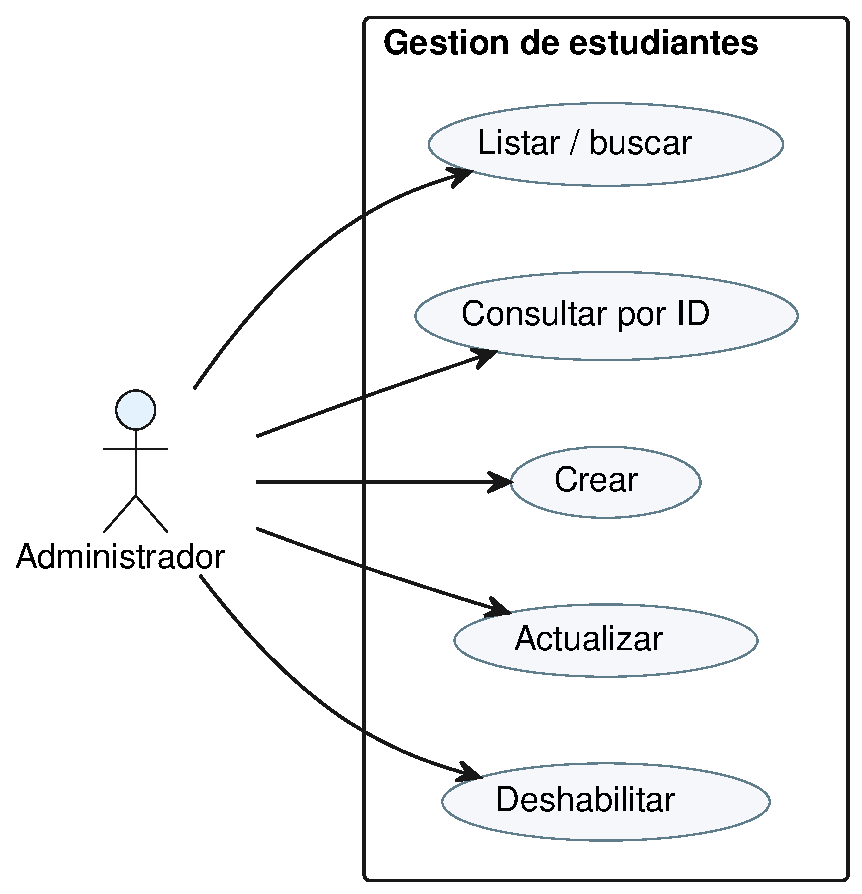
\includegraphics[width=\linewidth,height=0.30\textheight,keepaspectratio]{cu/cu05-uc.pdf}\caption{Diagrama de caso de uso --- CU-05}\end{figure}
\begin{figure}[H]\centering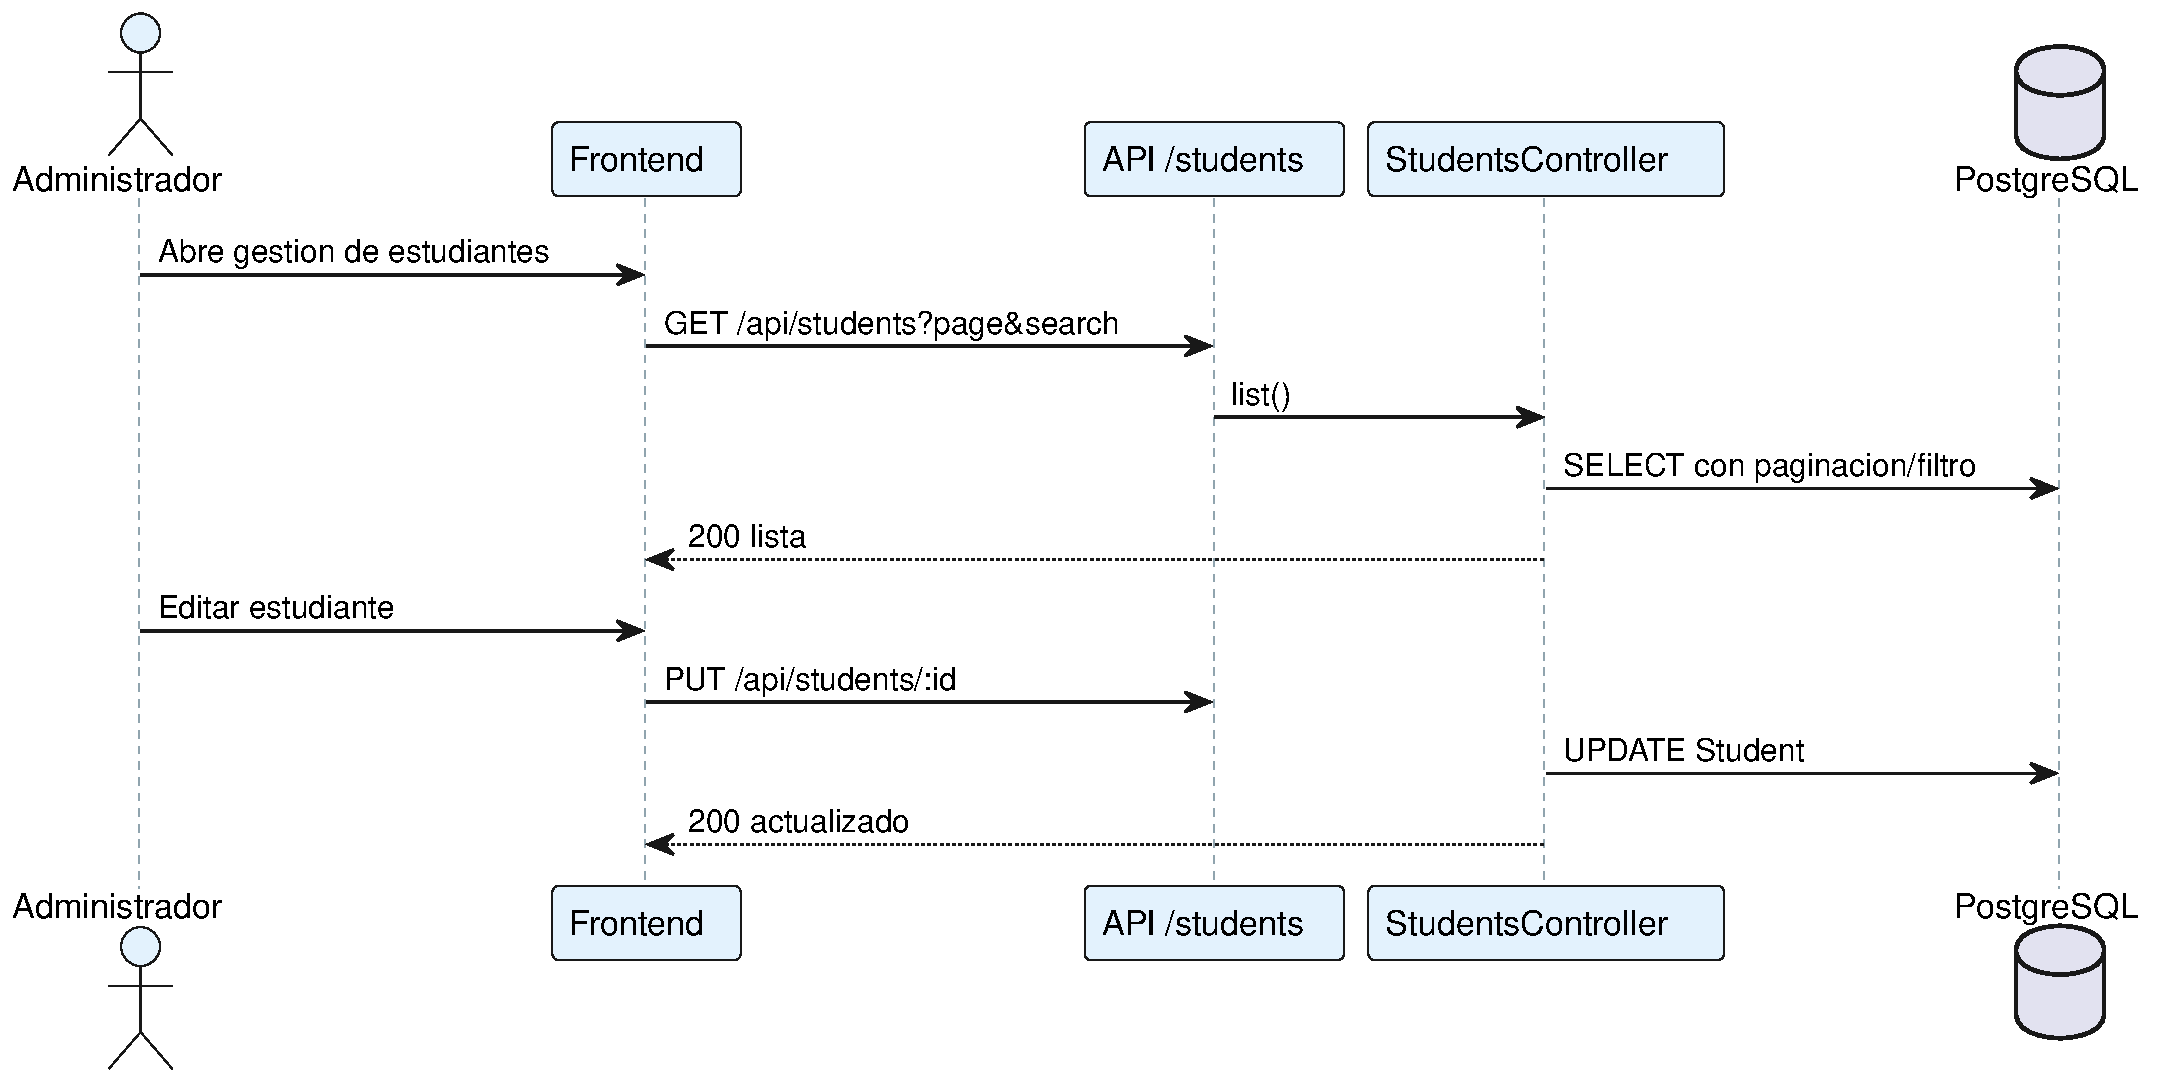
\includegraphics[width=\linewidth,height=0.42\textheight,keepaspectratio]{cu/cu05-seq.pdf}\caption{Diagrama de secuencia --- CU-05}\end{figure}
\begin{figure}[H]\centering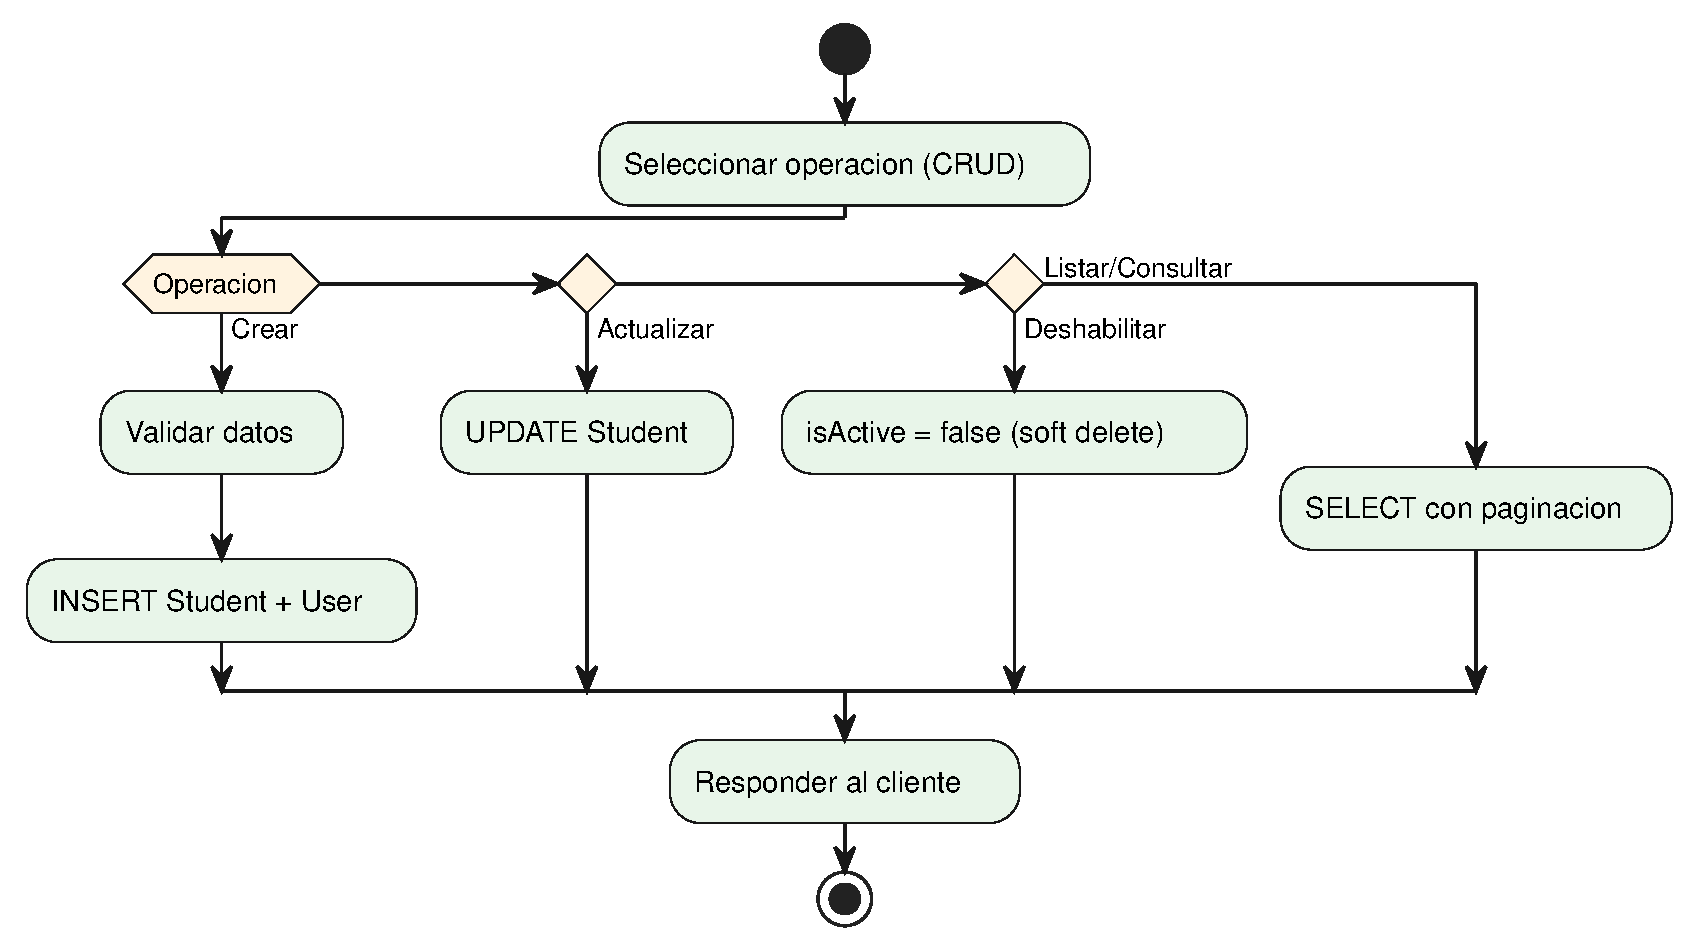
\includegraphics[width=\linewidth,height=0.46\textheight,keepaspectratio]{cu/cu05-act.pdf}\caption{Diagrama de actividades --- CU-05}\end{figure}

\subsection{CU-06 --- Importar estudiantes desde Excel}

\noindent\textbf{Endpoint(s):} \texttt{POST /api/students/import}\par\vspace{4pt}

\begin{table}[H]\centering\small
\caption{Ficha del caso de uso CU-06 --- Importar estudiantes desde Excel}
\begin{tabularx}{\textwidth}{L{0.26\textwidth} X}
\toprule
\textbf{Campo} & \textbf{Descripcion} \\ \midrule
Objetivo del contexto & Permitir al administrador cargar masivamente estudiantes a partir de un archivo Excel. \\ \midrule
Precondiciones & El administrador debe estar autenticado; el archivo debe tener el formato esperado. \\ \midrule
Condicion de exito & Se crean los estudiantes de las filas validas y se reporta el resultado. \\ \midrule
Condicion de fracaso & El archivo es invalido o no contiene filas procesables. \\ \midrule
Actores principales & Administrador \\ \midrule
Actores secundarios & Libreria de parseo xlsx \\
\bottomrule\end{tabularx}\end{table}
\begin{table}[H]\centering\small
\caption{Flujo principal de CU-06}
\begin{tabularx}{\textwidth}{C{0.10\textwidth} X}
\toprule \textbf{Paso} & \textbf{Accion} \\ \midrule
1 & El administrador sube un archivo .xlsx. \\
2 & El sistema parsea las filas del archivo. \\
3 & Por cada fila valida, el sistema crea el estudiante y su usuario. \\
4 & El sistema acumula errores de las filas invalidas. \\
5 & El sistema responde con un resumen (creados/errores). \\
\bottomrule\end{tabularx}\end{table}
\begin{table}[H]\centering\small
\caption{Extensiones (flujos alternativos) de CU-06}
\begin{tabularx}{\textwidth}{C{0.10\textwidth} X}
\toprule \textbf{Paso} & \textbf{Accion} \\ \midrule
2.1 & Archivo invalido o vacio $\rightarrow$ HTTP 400. \\
3.1 & Fila con datos invalidos $\rightarrow$ se registra el error y continua. \\
\bottomrule\end{tabularx}\end{table}
\begin{figure}[H]\centering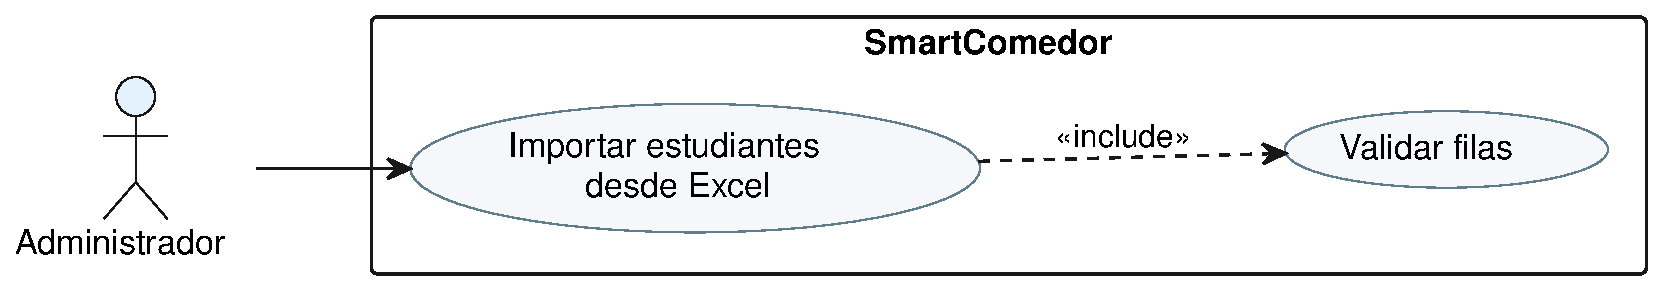
\includegraphics[width=\linewidth,height=0.30\textheight,keepaspectratio]{cu/cu06-uc.pdf}\caption{Diagrama de caso de uso --- CU-06}\end{figure}
\begin{figure}[H]\centering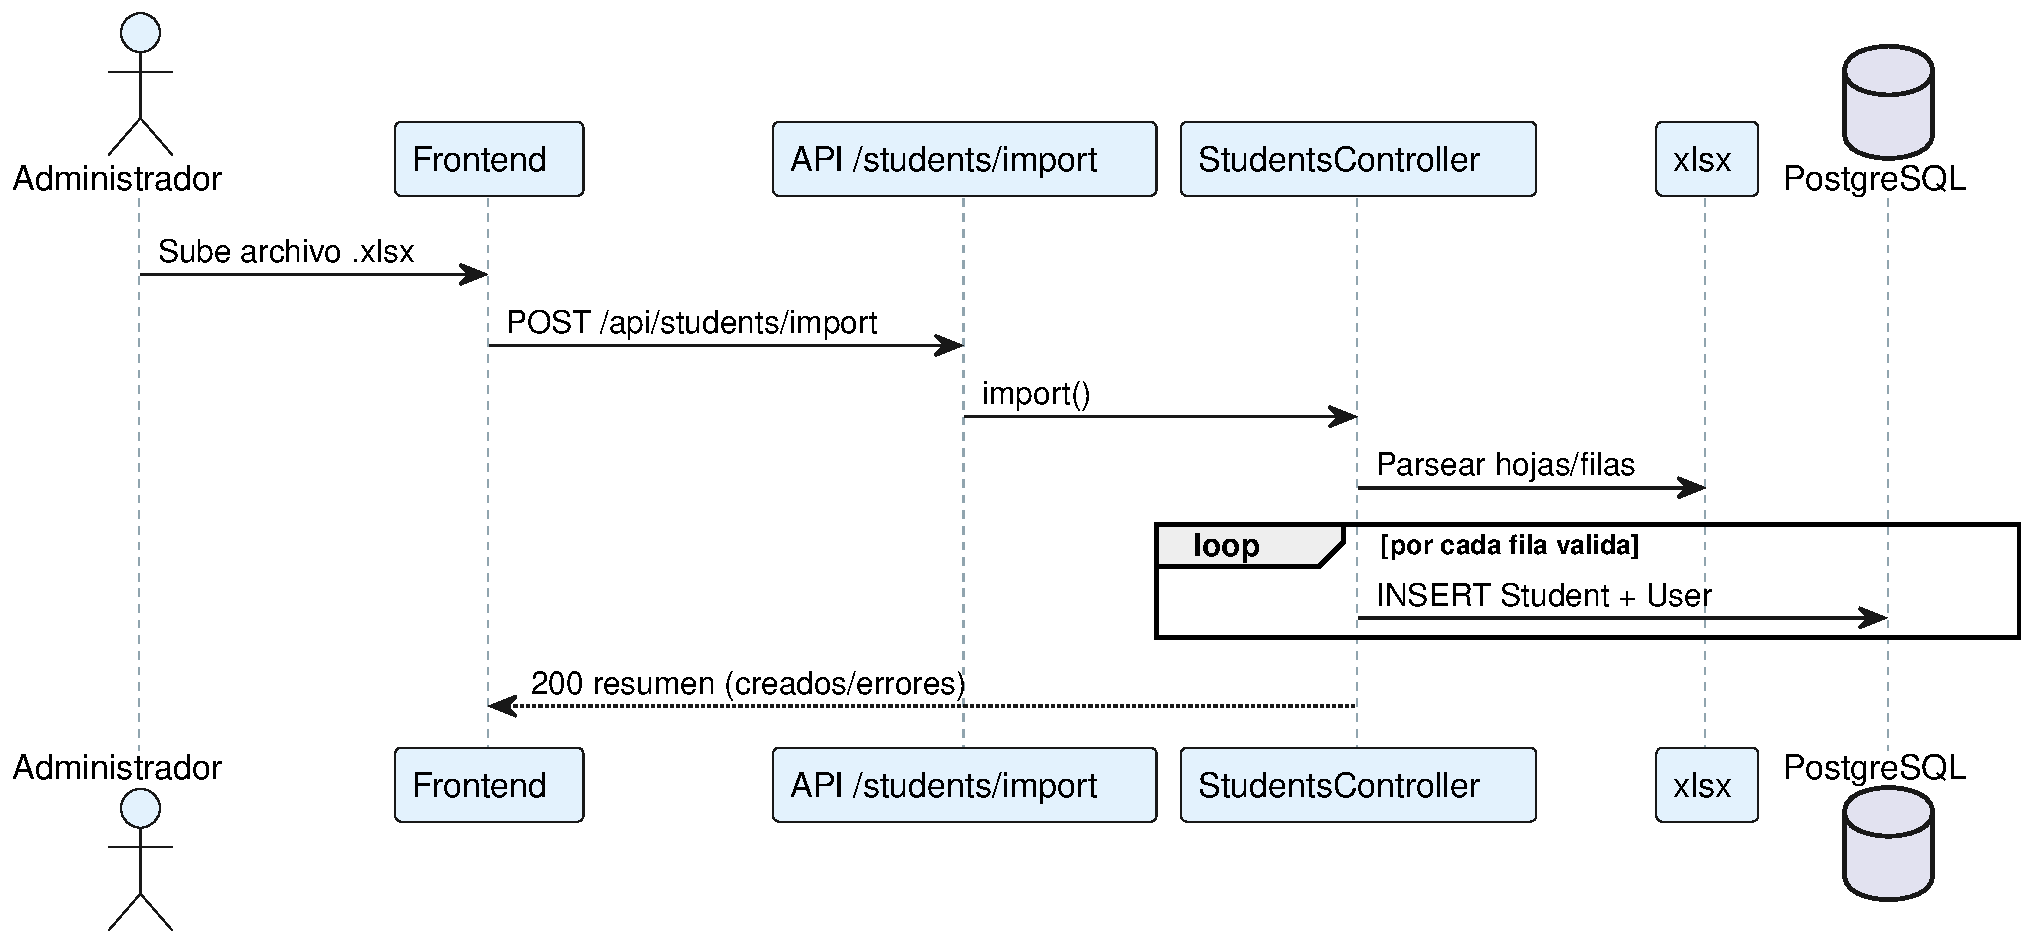
\includegraphics[width=\linewidth,height=0.42\textheight,keepaspectratio]{cu/cu06-seq.pdf}\caption{Diagrama de secuencia --- CU-06}\end{figure}
\begin{figure}[H]\centering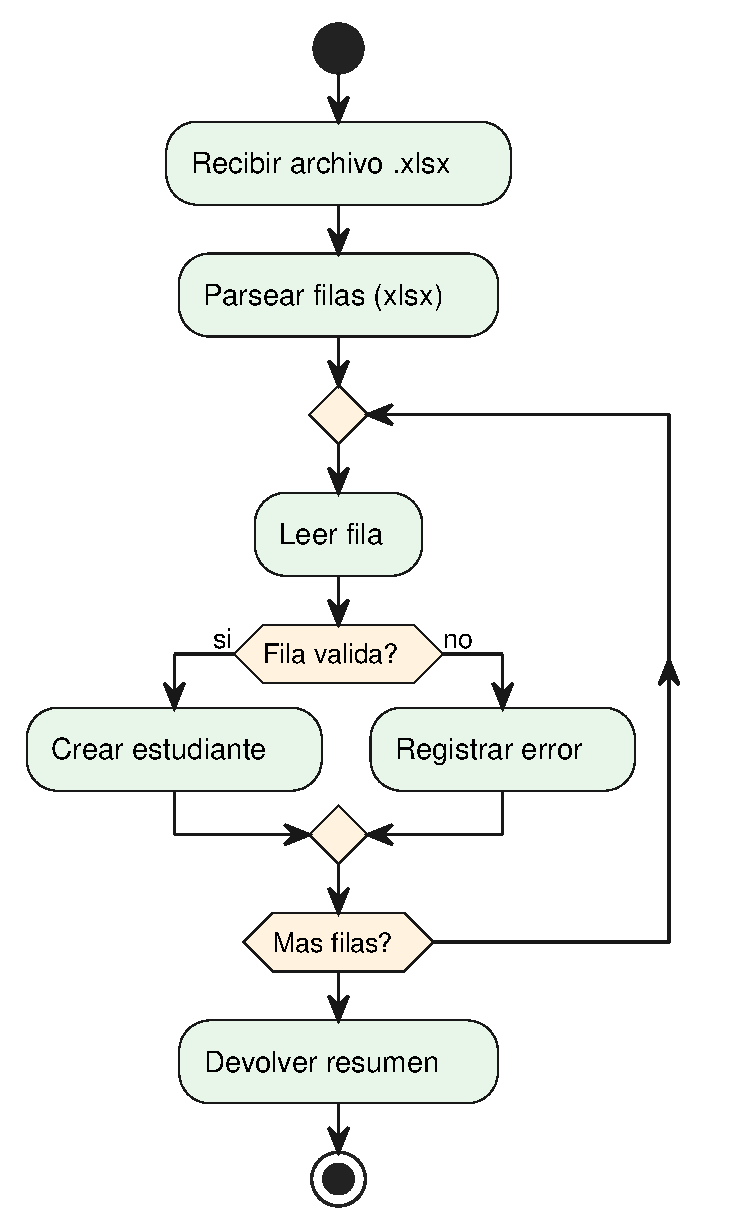
\includegraphics[width=\linewidth,height=0.46\textheight,keepaspectratio]{cu/cu06-act.pdf}\caption{Diagrama de actividades --- CU-06}\end{figure}

\subsection{CU-07 --- Validar SISBEN}

\noindent\textbf{Endpoint(s):} \texttt{POST /api/students/:id/validate-sisben}\par\vspace{4pt}

\begin{table}[H]\centering\small
\caption{Ficha del caso de uso CU-07 --- Validar SISBEN}
\begin{tabularx}{\textwidth}{L{0.26\textwidth} X}
\toprule
\textbf{Campo} & \textbf{Descripcion} \\ \midrule
Objetivo del contexto & Permitir al administrador validar la elegibilidad del estudiante cotejando el documento SISBEN con la cedula registrada. \\ \midrule
Precondiciones & El estudiante debe existir y tener documentos adjuntos. \\ \midrule
Condicion de exito & El estudiante queda con SISBEN validado. \\ \midrule
Condicion de fracaso & Existen discrepancias entre los documentos. \\ \midrule
Actores principales & Administrador \\ \midrule
Actores secundarios & Servicio de validacion SISBEN (PDF/OCR) \\
\bottomrule\end{tabularx}\end{table}
\begin{table}[H]\centering\small
\caption{Flujo principal de CU-07}
\begin{tabularx}{\textwidth}{C{0.10\textwidth} X}
\toprule \textbf{Paso} & \textbf{Accion} \\ \midrule
1 & El administrador solicita validar el SISBEN del estudiante. \\
2 & El sistema extrae el texto del documento (pdf-parse u OCR). \\
3 & El sistema normaliza y coteja cedula, nombre y apellido. \\
4 & Si todo coincide, marca isValidatedSisben = true y responde 200. \\
\bottomrule\end{tabularx}\end{table}
\begin{table}[H]\centering\small
\caption{Extensiones (flujos alternativos) de CU-07}
\begin{tabularx}{\textwidth}{C{0.10\textwidth} X}
\toprule \textbf{Paso} & \textbf{Accion} \\ \midrule
1.1 & Estudiante no encontrado $\rightarrow$ HTTP 404. \\
3.1 & Inconsistencia $\rightarrow$ validated=false con el detalle de cada discrepancia. \\
\bottomrule\end{tabularx}\end{table}
\begin{figure}[H]\centering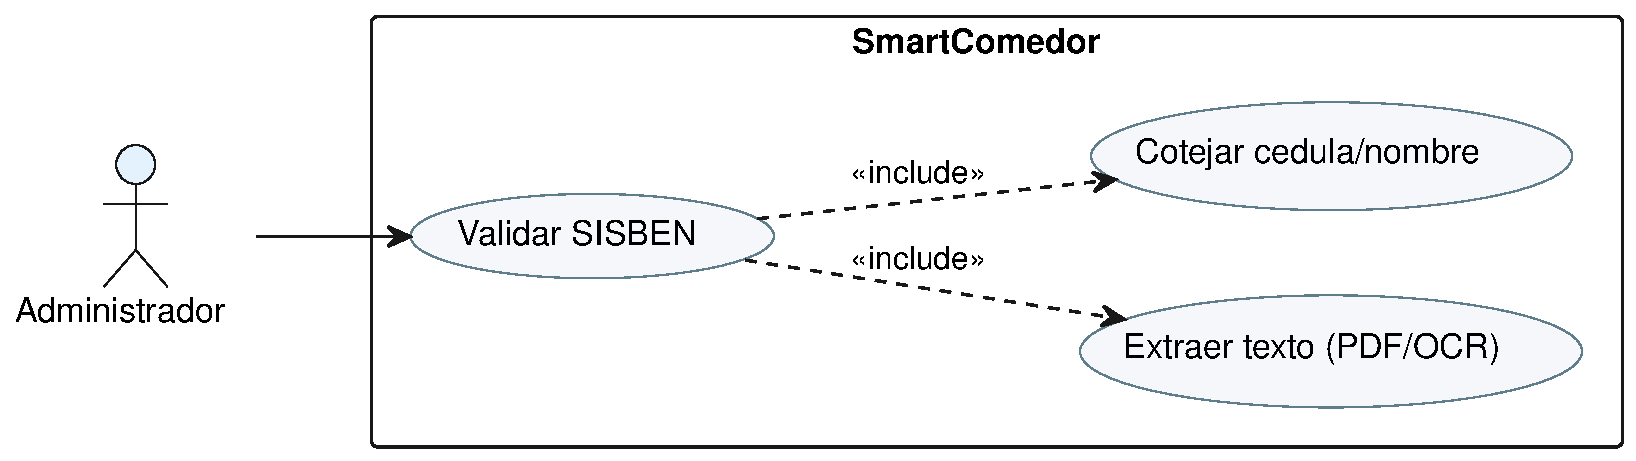
\includegraphics[width=\linewidth,height=0.30\textheight,keepaspectratio]{cu/cu07-uc.pdf}\caption{Diagrama de caso de uso --- CU-07}\end{figure}
\begin{figure}[H]\centering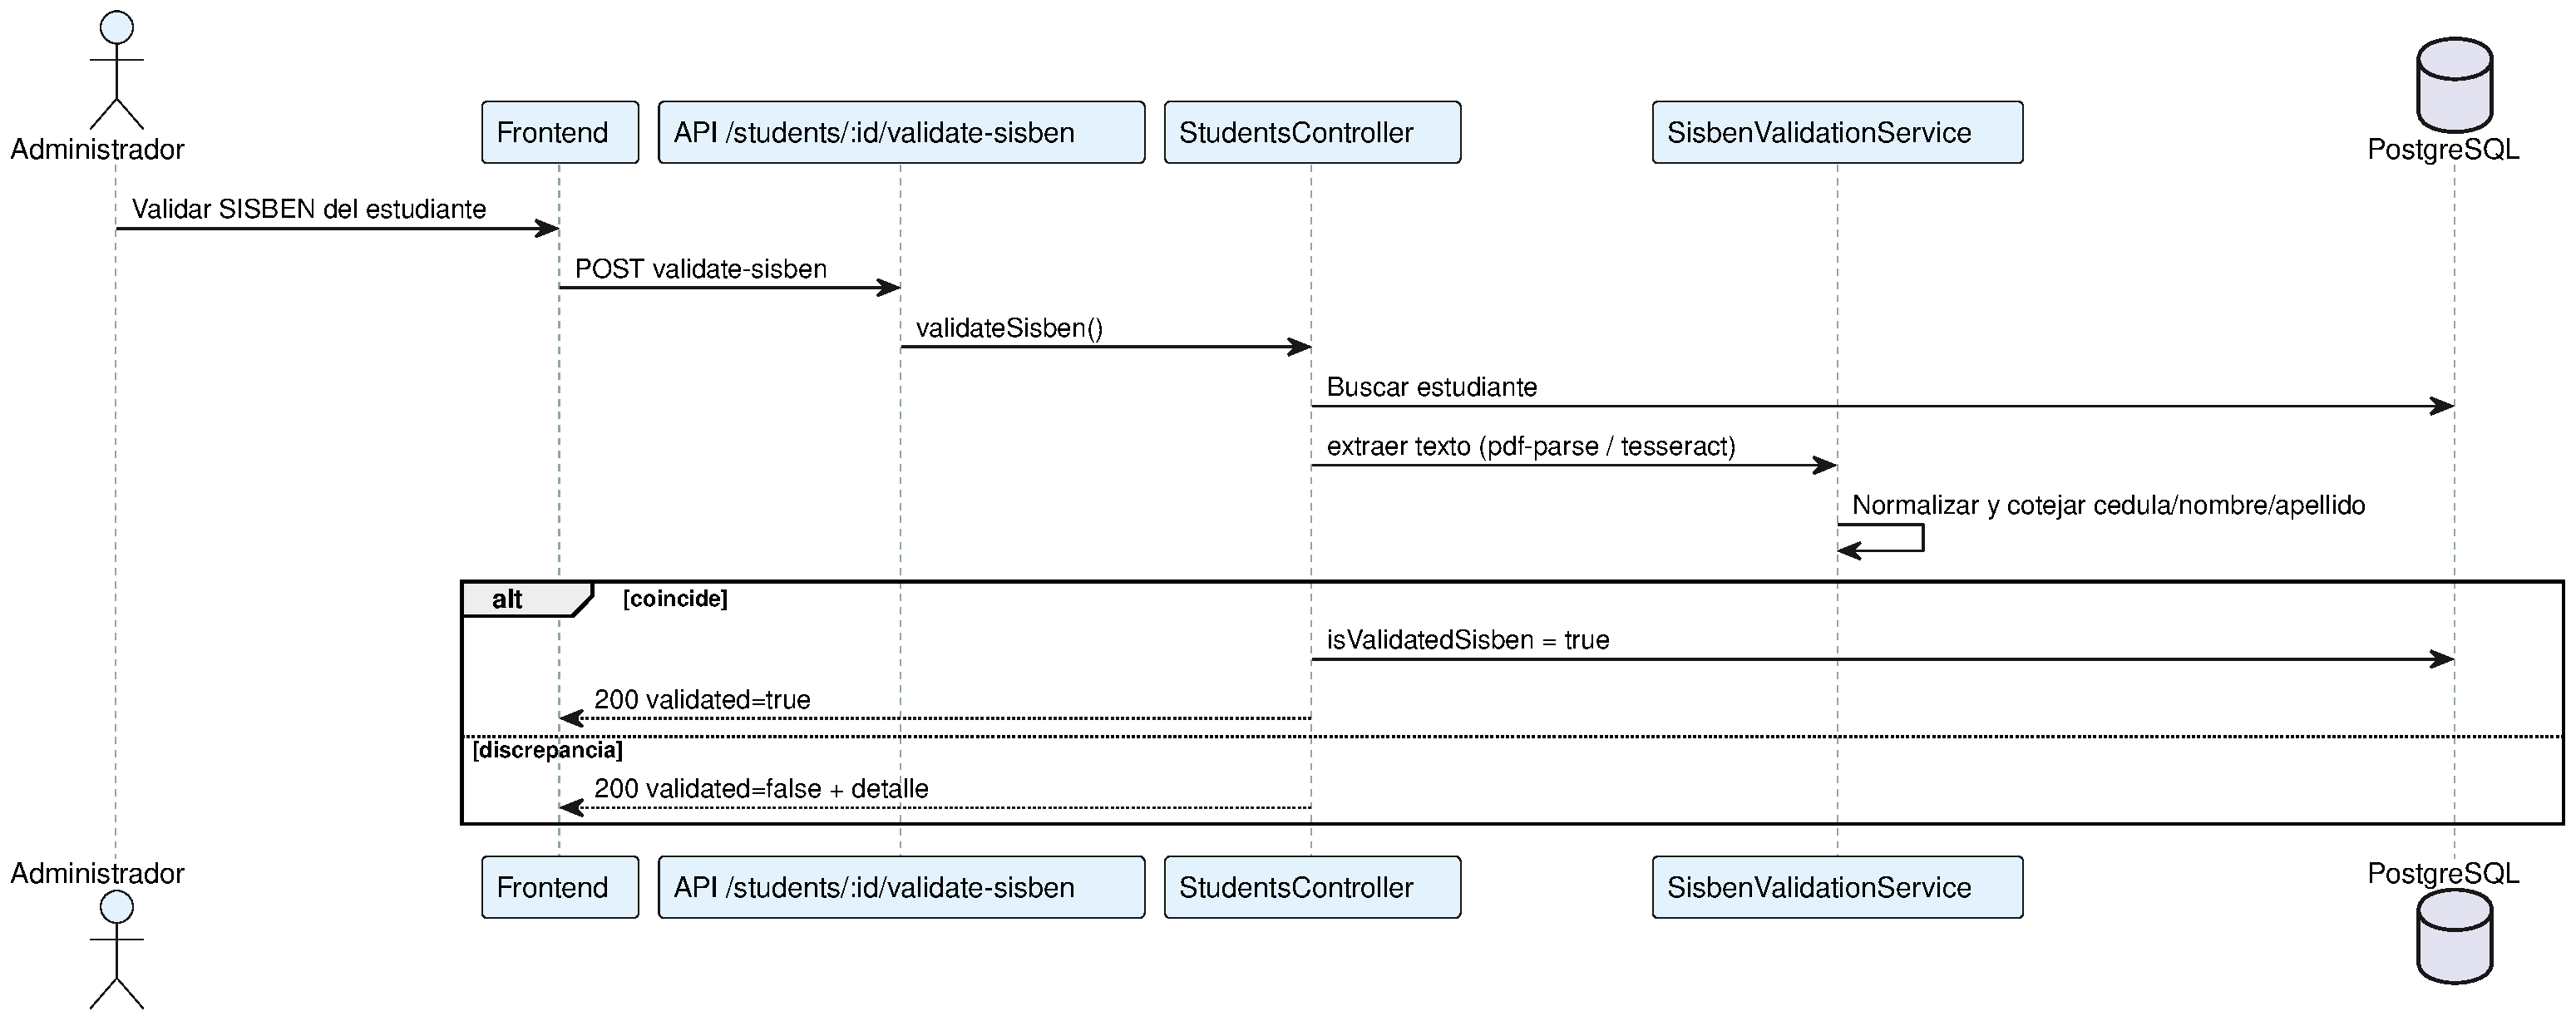
\includegraphics[width=\linewidth,height=0.42\textheight,keepaspectratio]{cu/cu07-seq.pdf}\caption{Diagrama de secuencia --- CU-07}\end{figure}
\begin{figure}[H]\centering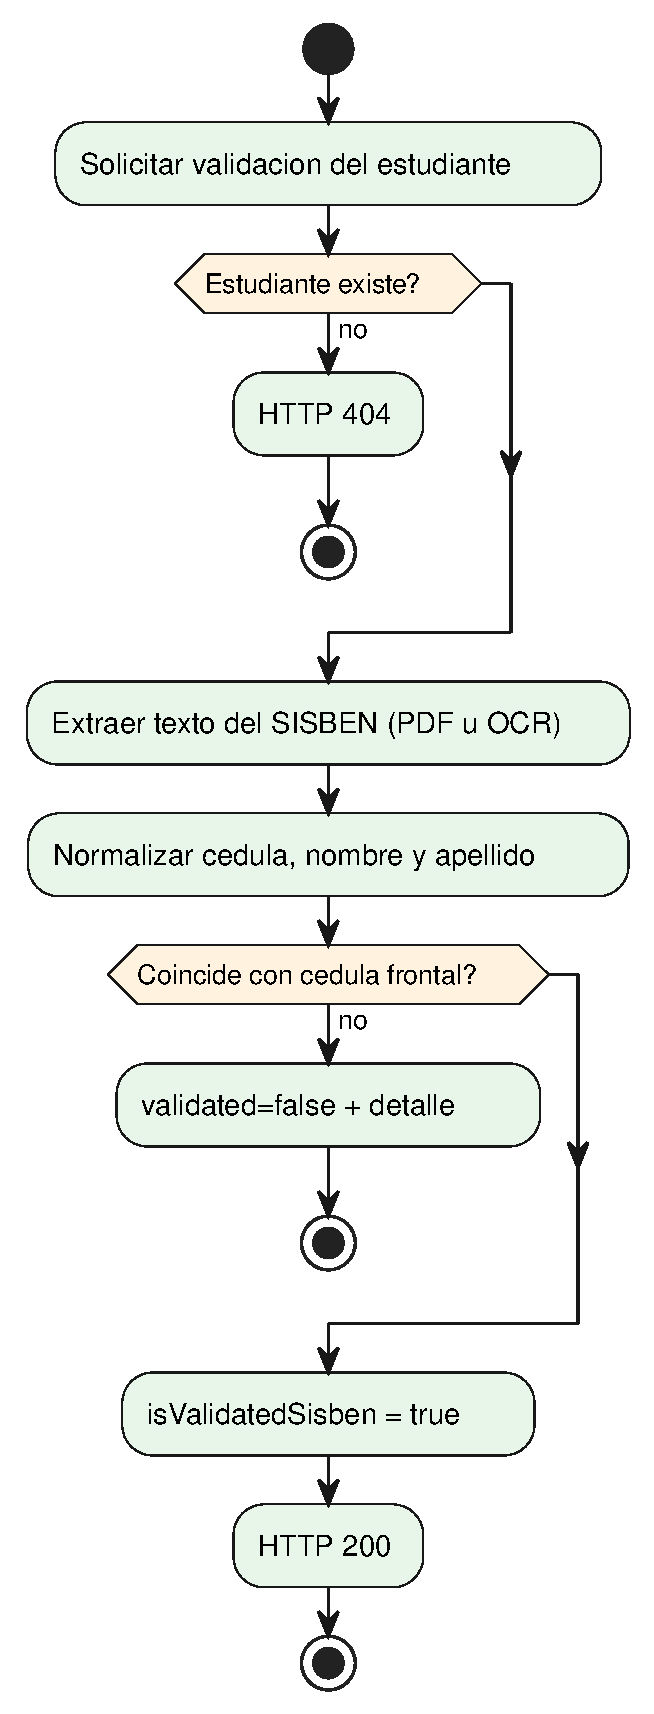
\includegraphics[width=\linewidth,height=0.46\textheight,keepaspectratio]{cu/cu07-act.pdf}\caption{Diagrama de actividades --- CU-07}\end{figure}

\subsection{CU-08 --- Gestionar supervisores}

\noindent\textbf{Endpoint(s):} \texttt{GET/POST/PUT/PATCH/DELETE /api/supervisors}\par\vspace{4pt}

\begin{table}[H]\centering\small
\caption{Ficha del caso de uso CU-08 --- Gestionar supervisores}
\begin{tabularx}{\textwidth}{L{0.26\textwidth} X}
\toprule
\textbf{Campo} & \textbf{Descripcion} \\ \midrule
Objetivo del contexto & Permitir al administrador crear, actualizar, cambiar de estado y deshabilitar supervisores, y consultar sus bitacoras. \\ \midrule
Precondiciones & El administrador debe estar autenticado con rol admin. \\ \midrule
Condicion de exito & El supervisor se crea o actualiza segun la operacion. \\ \midrule
Condicion de fracaso & Datos invalidos o supervisor inexistente. \\ \midrule
Actores principales & Administrador \\ \midrule
Actores secundarios & Base de datos \\
\bottomrule\end{tabularx}\end{table}
\begin{table}[H]\centering\small
\caption{Flujo principal de CU-08}
\begin{tabularx}{\textwidth}{C{0.10\textwidth} X}
\toprule \textbf{Paso} & \textbf{Accion} \\ \midrule
1 & El administrador selecciona la operacion sobre el supervisor. \\
2 & Para crear, el sistema genera una contrasena temporal cifrada. \\
3 & El sistema persiste el usuario con rol supervisor. \\
4 & Para cambiar estado, actualiza isActive/isAuthorized. \\
5 & El sistema responde con el resultado. \\
\bottomrule\end{tabularx}\end{table}
\begin{table}[H]\centering\small
\caption{Extensiones (flujos alternativos) de CU-08}
\begin{tabularx}{\textwidth}{C{0.10\textwidth} X}
\toprule \textbf{Paso} & \textbf{Accion} \\ \midrule
3.1 & Correo duplicado $\rightarrow$ HTTP 400. \\
4.1 & Supervisor inexistente $\rightarrow$ HTTP 404. \\
\bottomrule\end{tabularx}\end{table}
\begin{figure}[H]\centering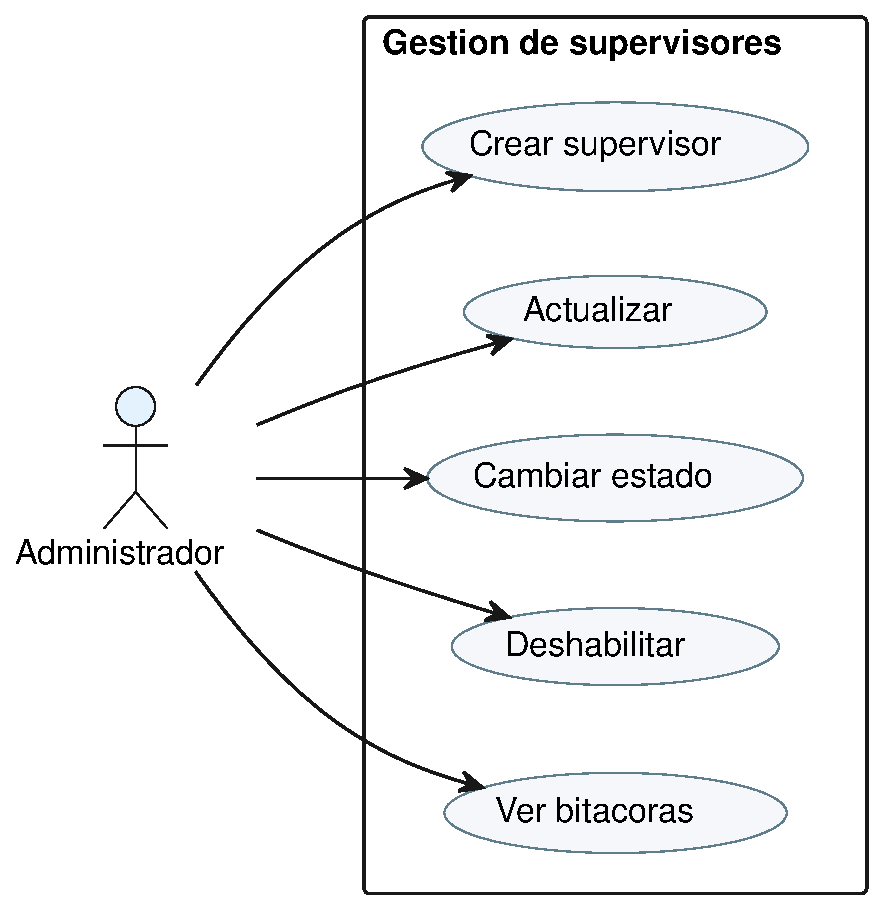
\includegraphics[width=\linewidth,height=0.30\textheight,keepaspectratio]{cu/cu08-uc.pdf}\caption{Diagrama de caso de uso --- CU-08}\end{figure}
\begin{figure}[H]\centering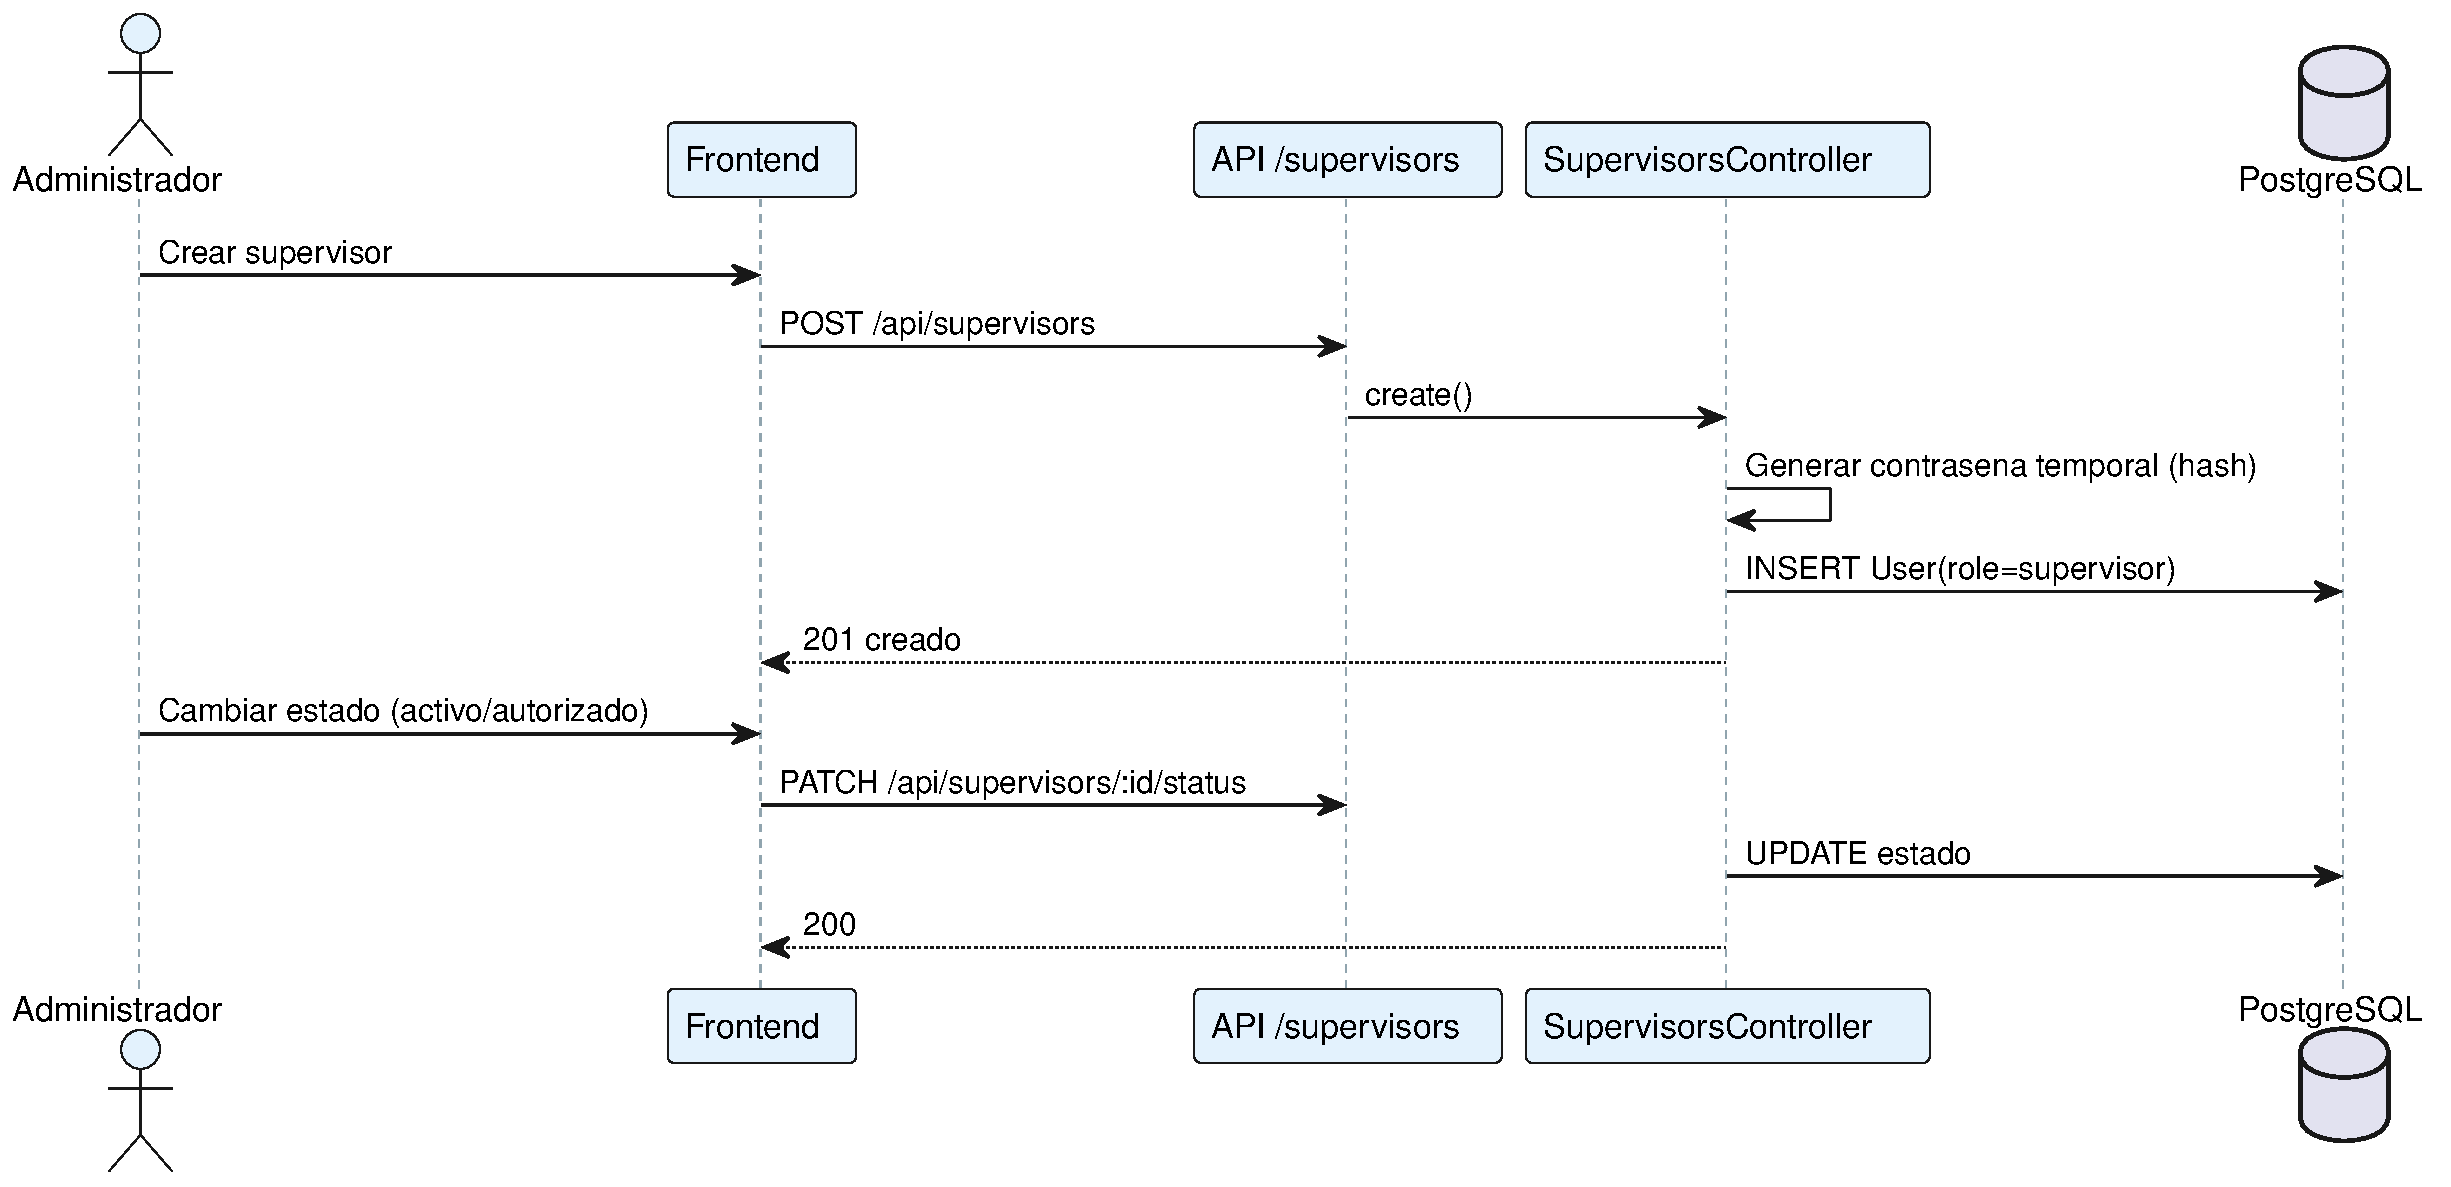
\includegraphics[width=\linewidth,height=0.42\textheight,keepaspectratio]{cu/cu08-seq.pdf}\caption{Diagrama de secuencia --- CU-08}\end{figure}
\begin{figure}[H]\centering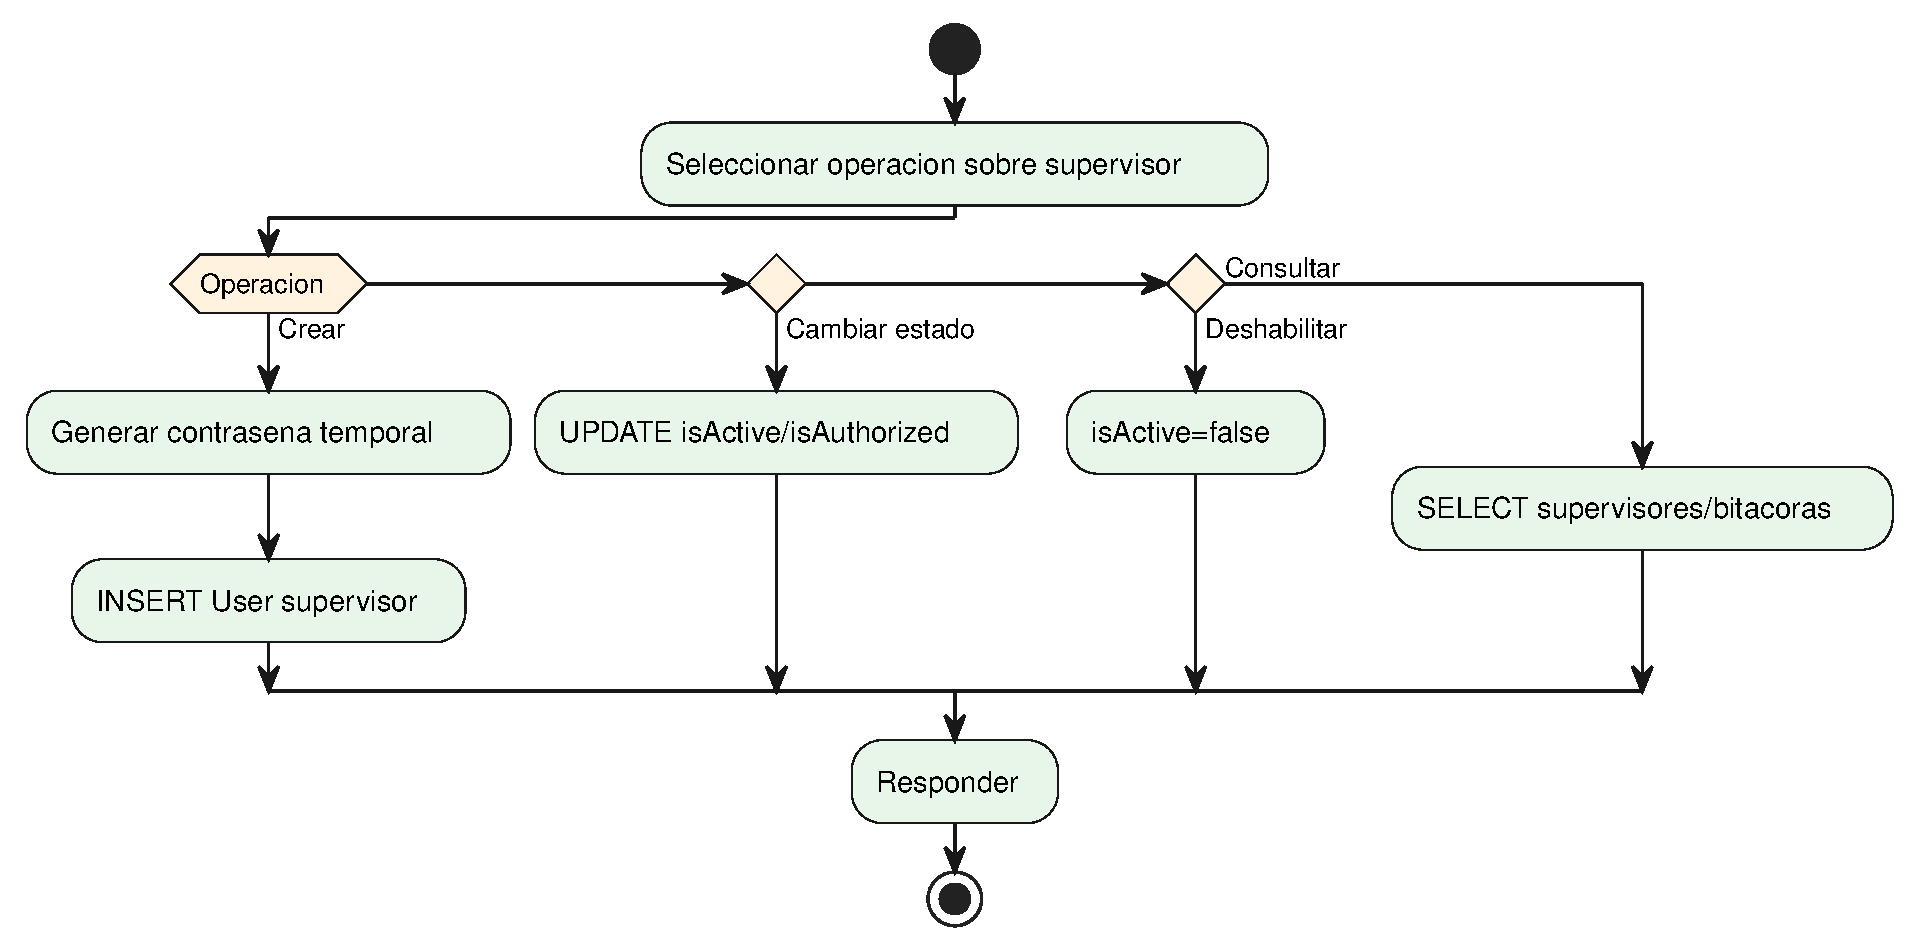
\includegraphics[width=\linewidth,height=0.46\textheight,keepaspectratio]{cu/cu08-act.pdf}\caption{Diagrama de actividades --- CU-08}\end{figure}

\subsection{CU-09 --- Invitar supervisor / unirse por invitacion}

\noindent\textbf{Endpoint(s):} \texttt{POST /api/supervisors/invite, POST /api/supervisors/join}\par\vspace{4pt}

\begin{table}[H]\centering\small
\caption{Ficha del caso de uso CU-09 --- Invitar supervisor / unirse por invitacion}
\begin{tabularx}{\textwidth}{L{0.26\textwidth} X}
\toprule
\textbf{Campo} & \textbf{Descripcion} \\ \midrule
Objetivo del contexto & Permitir al administrador invitar supervisores por correo y a estos crear su cuenta mediante un enlace temporal. \\ \midrule
Precondiciones & El administrador debe estar autenticado; la invitacion debe estar vigente. \\ \midrule
Condicion de exito & El supervisor crea su cuenta a partir de la invitacion. \\ \midrule
Condicion de fracaso & El token de invitacion es invalido o expirado. \\ \midrule
Actores principales & Administrador, Supervisor \\ \midrule
Actores secundarios & Servicio de correo \\
\bottomrule\end{tabularx}\end{table}
\begin{table}[H]\centering\small
\caption{Flujo principal de CU-09}
\begin{tabularx}{\textwidth}{C{0.10\textwidth} X}
\toprule \textbf{Paso} & \textbf{Accion} \\ \midrule
1 & El administrador genera una invitacion indicando el correo. \\
2 & El sistema crea un token con vigencia de 48 horas. \\
3 & El sistema envia el enlace de invitacion por correo. \\
4 & El supervisor abre el enlace y completa sus datos. \\
5 & El sistema valida el token y crea la cuenta de supervisor. \\
\bottomrule\end{tabularx}\end{table}
\begin{table}[H]\centering\small
\caption{Extensiones (flujos alternativos) de CU-09}
\begin{tabularx}{\textwidth}{C{0.10\textwidth} X}
\toprule \textbf{Paso} & \textbf{Accion} \\ \midrule
5.1 & Token vencido $\rightarrow$ HTTP 400. \\
5.2 & Correo duplicado $\rightarrow$ HTTP 400. \\
\bottomrule\end{tabularx}\end{table}
\begin{figure}[H]\centering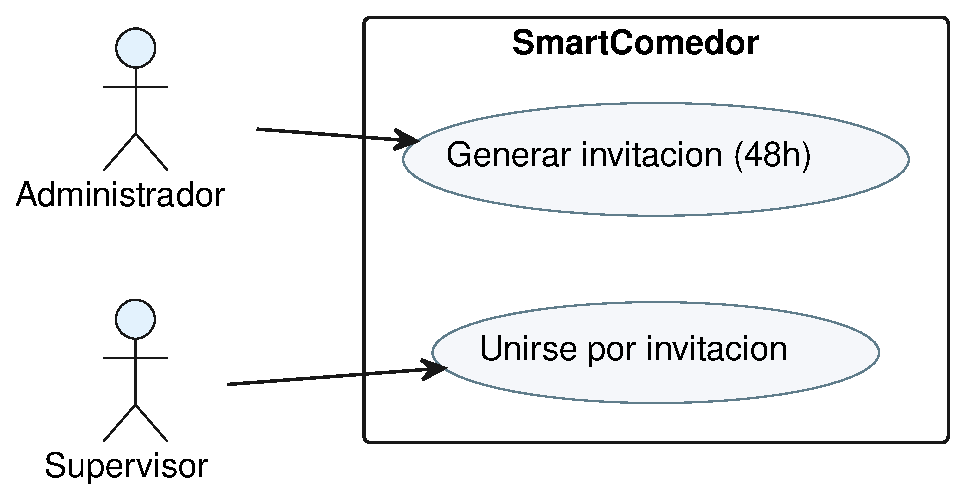
\includegraphics[width=\linewidth,height=0.30\textheight,keepaspectratio]{cu/cu09-uc.pdf}\caption{Diagrama de caso de uso --- CU-09}\end{figure}
\begin{figure}[H]\centering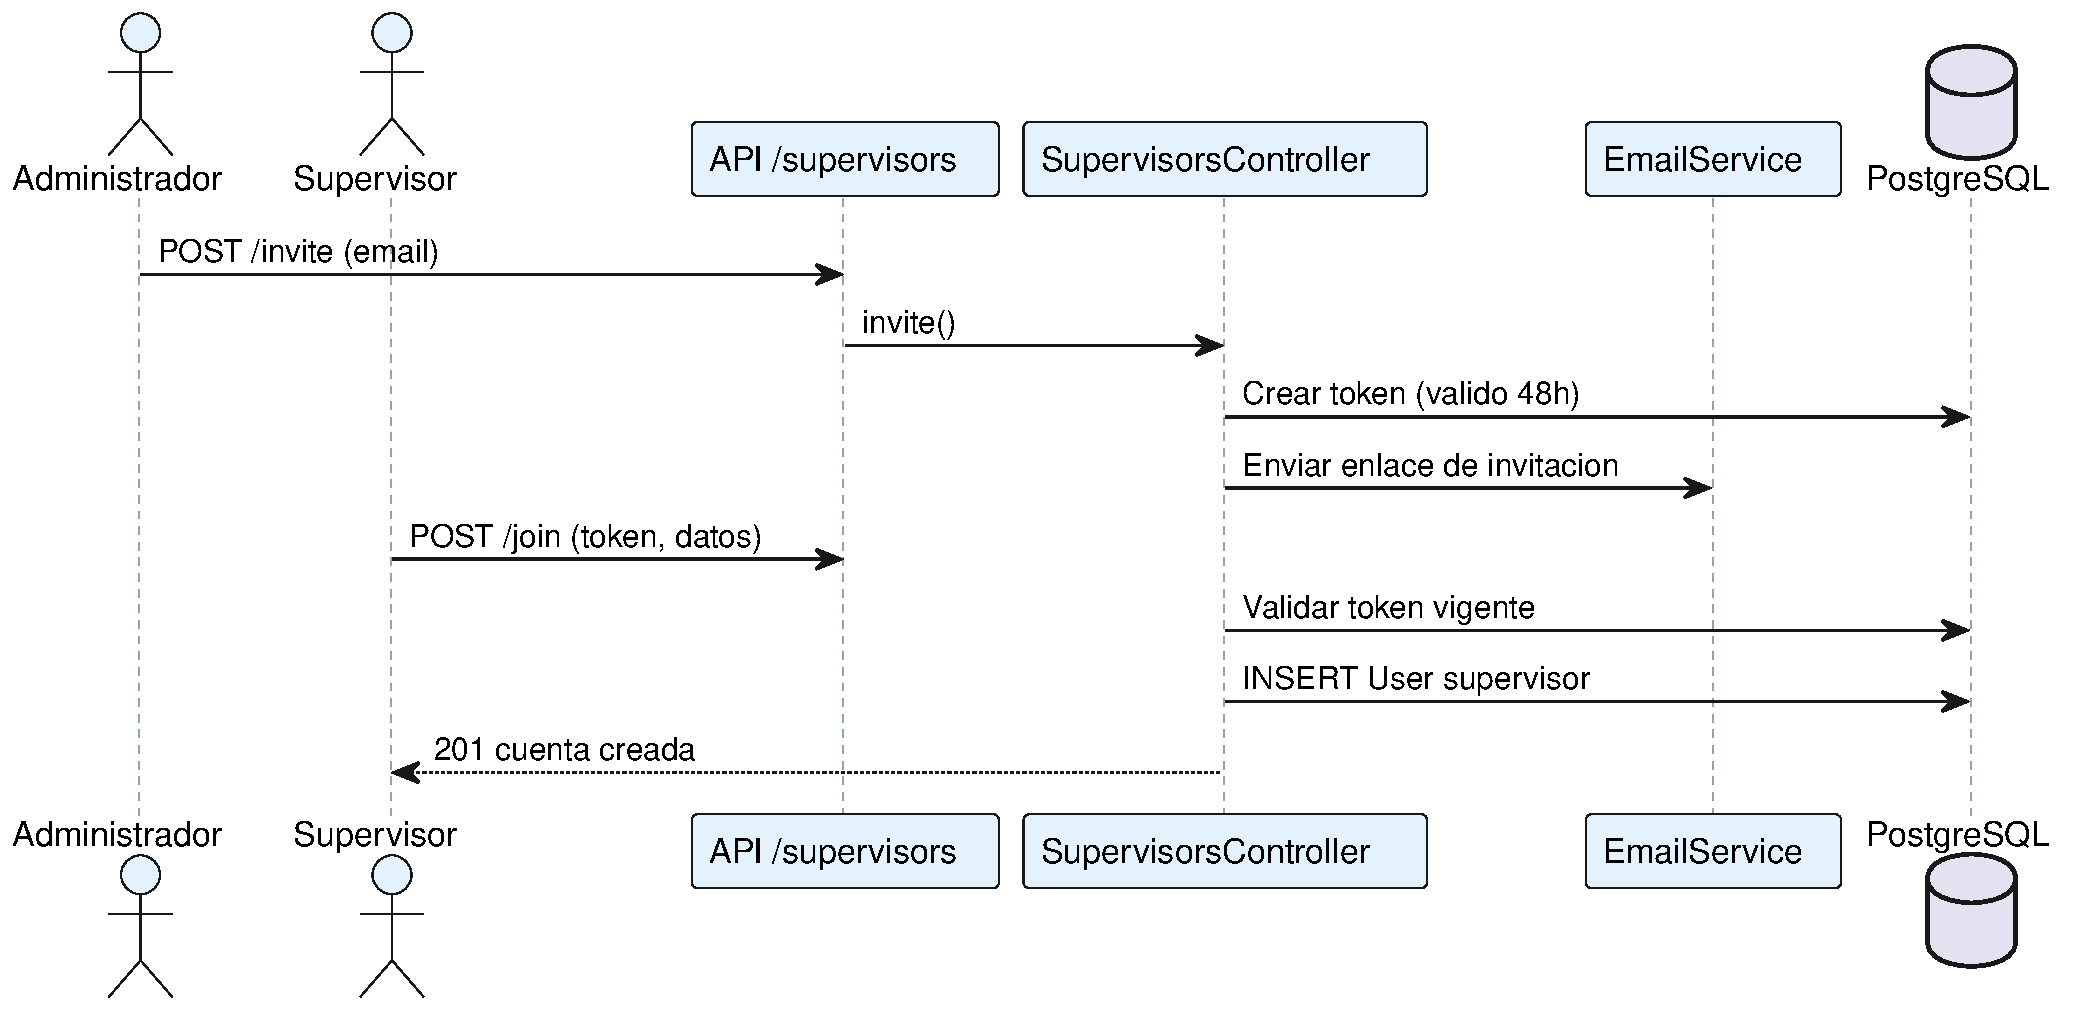
\includegraphics[width=\linewidth,height=0.42\textheight,keepaspectratio]{cu/cu09-seq.pdf}\caption{Diagrama de secuencia --- CU-09}\end{figure}
\begin{figure}[H]\centering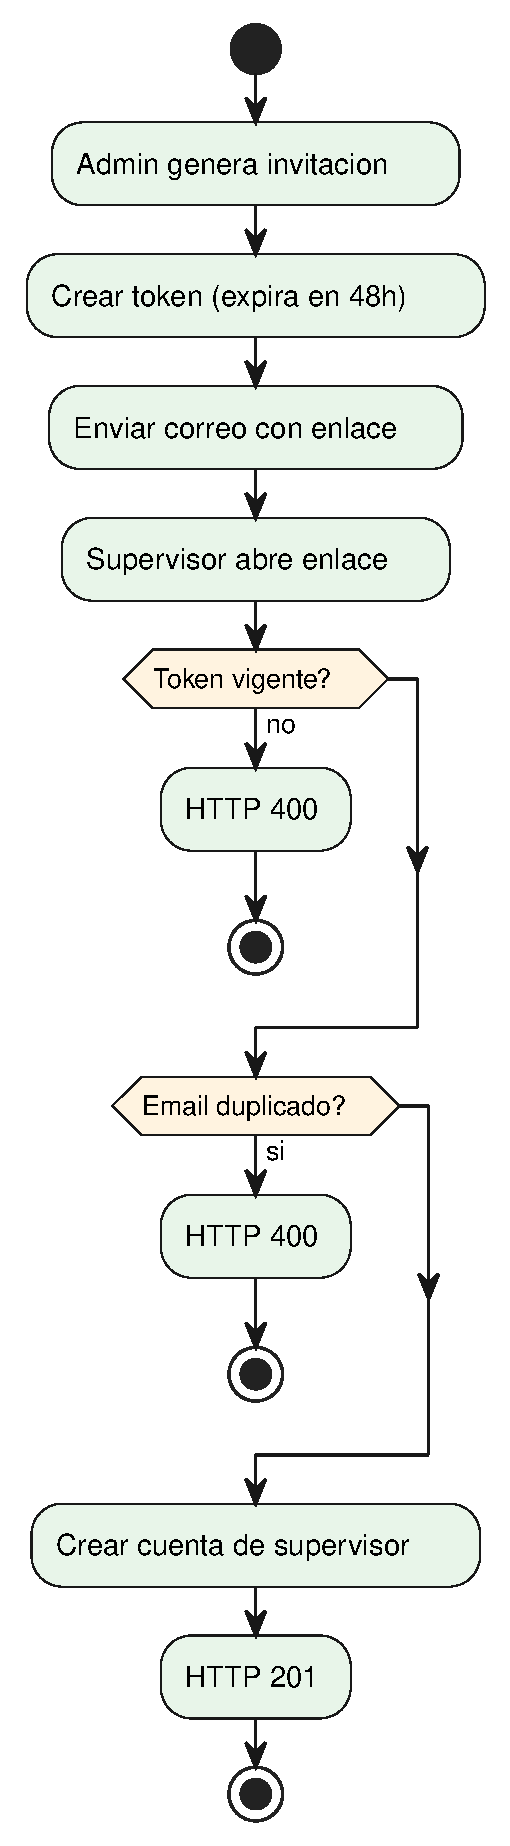
\includegraphics[width=\linewidth,height=0.46\textheight,keepaspectratio]{cu/cu09-act.pdf}\caption{Diagrama de actividades --- CU-09}\end{figure}

\subsection{CU-10 --- Asignar estudiantes a supervisor}

\noindent\textbf{Endpoint(s):} \texttt{POST/DELETE /api/supervisors/:id/assignments}\par\vspace{4pt}

\begin{table}[H]\centering\small
\caption{Ficha del caso de uso CU-10 --- Asignar estudiantes a supervisor}
\begin{tabularx}{\textwidth}{L{0.26\textwidth} X}
\toprule
\textbf{Campo} & \textbf{Descripcion} \\ \midrule
Objetivo del contexto & Permitir al administrador asociar estudiantes a un supervisor para delimitar su ambito de supervision. \\ \midrule
Precondiciones & El supervisor y el estudiante deben existir. \\ \midrule
Condicion de exito & Se crea la relacion supervisor-estudiante. \\ \midrule
Condicion de fracaso & La asignacion ya existe. \\ \midrule
Actores principales & Administrador \\ \midrule
Actores secundarios & Base de datos \\
\bottomrule\end{tabularx}\end{table}
\begin{table}[H]\centering\small
\caption{Flujo principal de CU-10}
\begin{tabularx}{\textwidth}{C{0.10\textwidth} X}
\toprule \textbf{Paso} & \textbf{Accion} \\ \midrule
1 & El administrador selecciona un supervisor y un estudiante. \\
2 & El sistema verifica que la asignacion no exista. \\
3 & El sistema crea el registro de asignacion (N:M). \\
4 & El sistema responde 201. \\
\bottomrule\end{tabularx}\end{table}
\begin{table}[H]\centering\small
\caption{Extensiones (flujos alternativos) de CU-10}
\begin{tabularx}{\textwidth}{C{0.10\textwidth} X}
\toprule \textbf{Paso} & \textbf{Accion} \\ \midrule
2.1 & Asignacion duplicada $\rightarrow$ HTTP 400. \\
\bottomrule\end{tabularx}\end{table}
\begin{figure}[H]\centering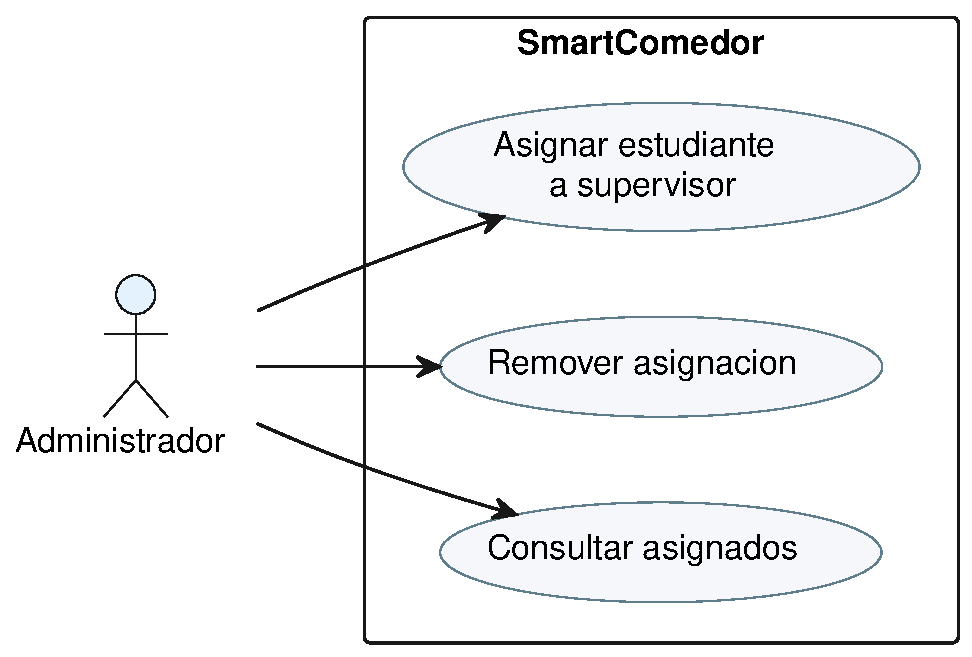
\includegraphics[width=\linewidth,height=0.30\textheight,keepaspectratio]{cu/cu10-uc.pdf}\caption{Diagrama de caso de uso --- CU-10}\end{figure}
\begin{figure}[H]\centering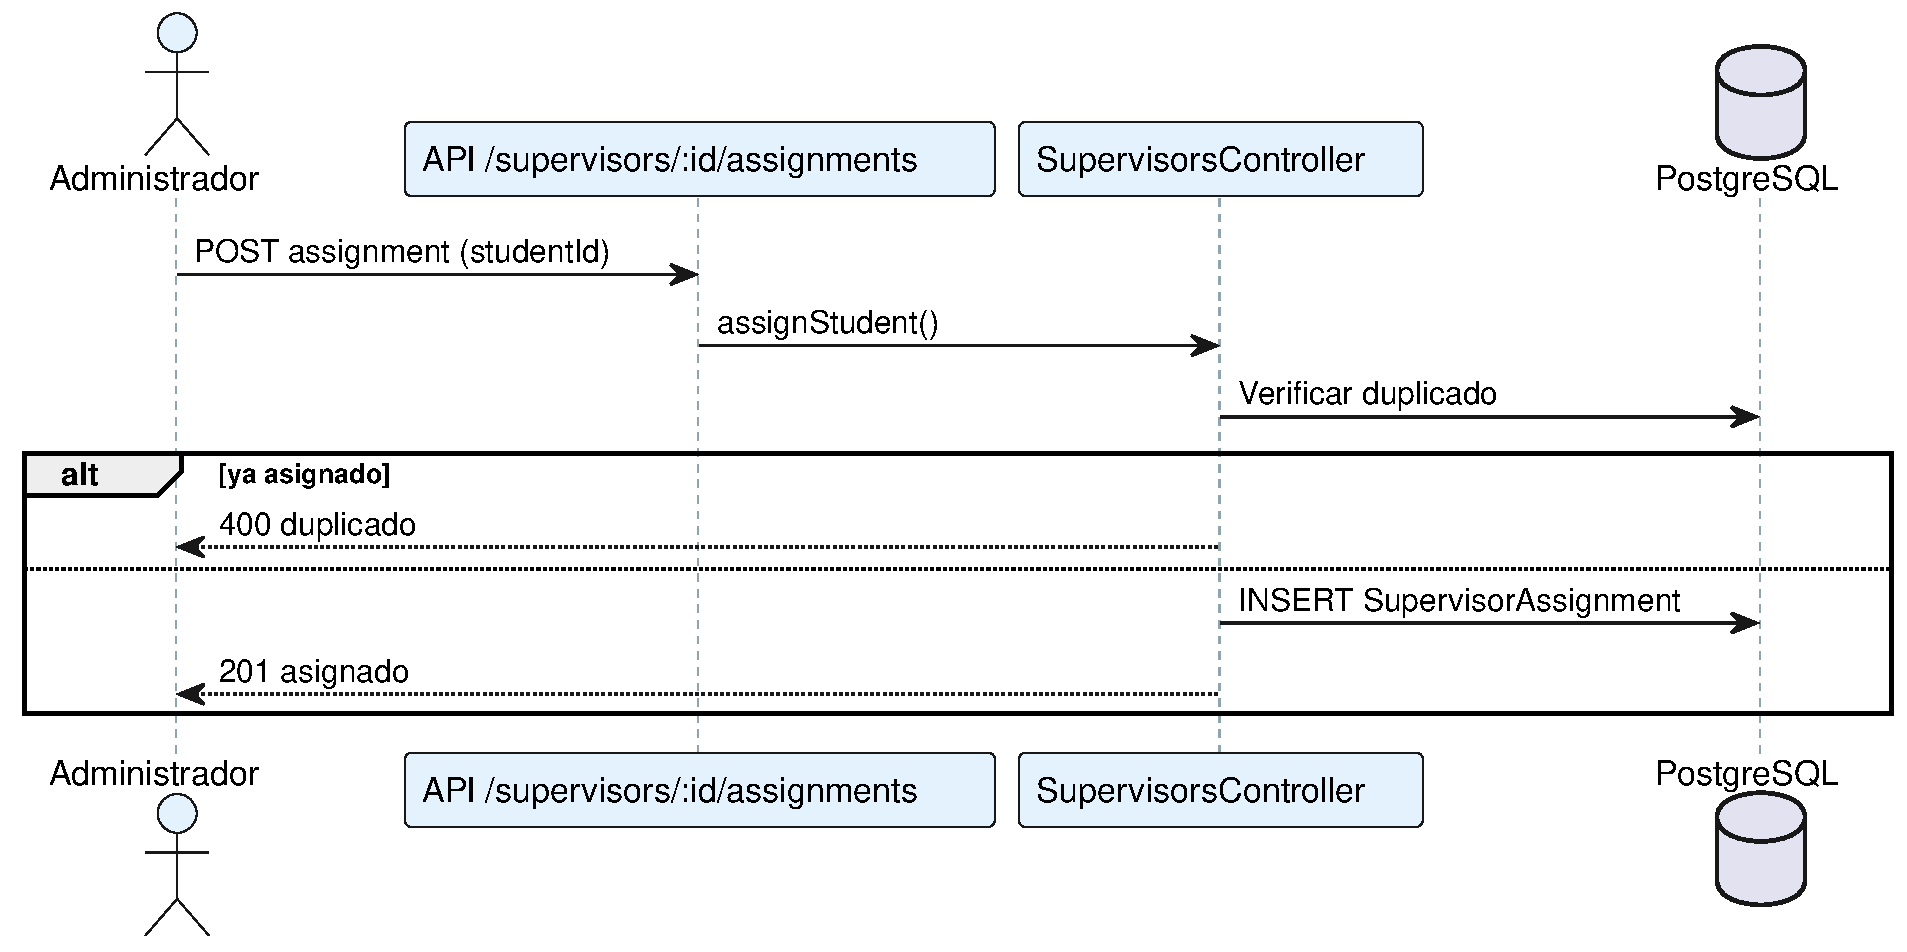
\includegraphics[width=\linewidth,height=0.42\textheight,keepaspectratio]{cu/cu10-seq.pdf}\caption{Diagrama de secuencia --- CU-10}\end{figure}
\begin{figure}[H]\centering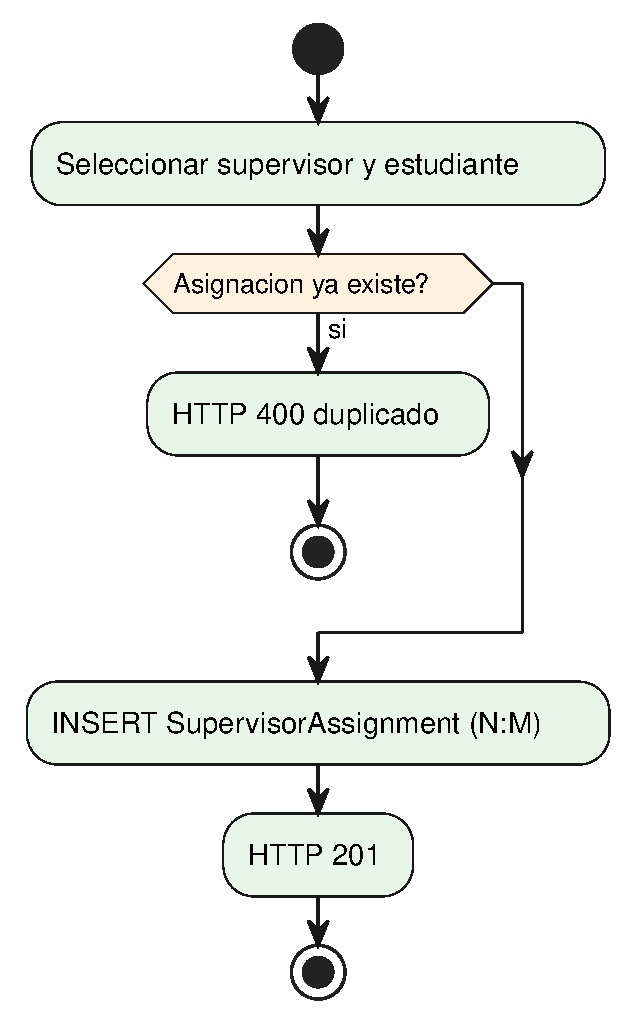
\includegraphics[width=\linewidth,height=0.46\textheight,keepaspectratio]{cu/cu10-act.pdf}\caption{Diagrama de actividades --- CU-10}\end{figure}

\subsection{CU-11 --- Subir pago y comprobantes}

\noindent\textbf{Endpoint(s):} \texttt{POST /api/payments, POST /api/payments/upload, POST /api/payments/calculate}\par\vspace{4pt}

\begin{table}[H]\centering\small
\caption{Ficha del caso de uso CU-11 --- Subir pago y comprobantes}
\begin{tabularx}{\textwidth}{L{0.26\textwidth} X}
\toprule
\textbf{Campo} & \textbf{Descripcion} \\ \midrule
Objetivo del contexto & Permitir al estudiante registrar un pago/recarga indicando el monto y adjuntando el comprobante, calculando los almuerzos incluidos. \\ \midrule
Precondiciones & El estudiante debe estar autenticado. \\ \midrule
Condicion de exito & Se crea un pago pendiente de verificacion con los almuerzos calculados. \\ \midrule
Condicion de fracaso & El monto es invalido (menor al precio de un almuerzo). \\ \midrule
Actores principales & Estudiante \\ \midrule
Actores secundarios & Almacenamiento de archivos \\
\bottomrule\end{tabularx}\end{table}
\begin{table}[H]\centering\small
\caption{Flujo principal de CU-11}
\begin{tabularx}{\textwidth}{C{0.10\textwidth} X}
\toprule \textbf{Paso} & \textbf{Accion} \\ \midrule
1 & El estudiante ingresa el monto y adjunta el comprobante. \\
2 & El sistema calcula almuerzos = piso(monto/2000). \\
3 & El sistema crea el pago con isVerified=false. \\
4 & El sistema responde 201. \\
\bottomrule\end{tabularx}\end{table}
\begin{table}[H]\centering\small
\caption{Extensiones (flujos alternativos) de CU-11}
\begin{tabularx}{\textwidth}{C{0.10\textwidth} X}
\toprule \textbf{Paso} & \textbf{Accion} \\ \midrule
2.1 & Monto menor a 2000 $\rightarrow$ HTTP 400. \\
\bottomrule\end{tabularx}\end{table}
\begin{figure}[H]\centering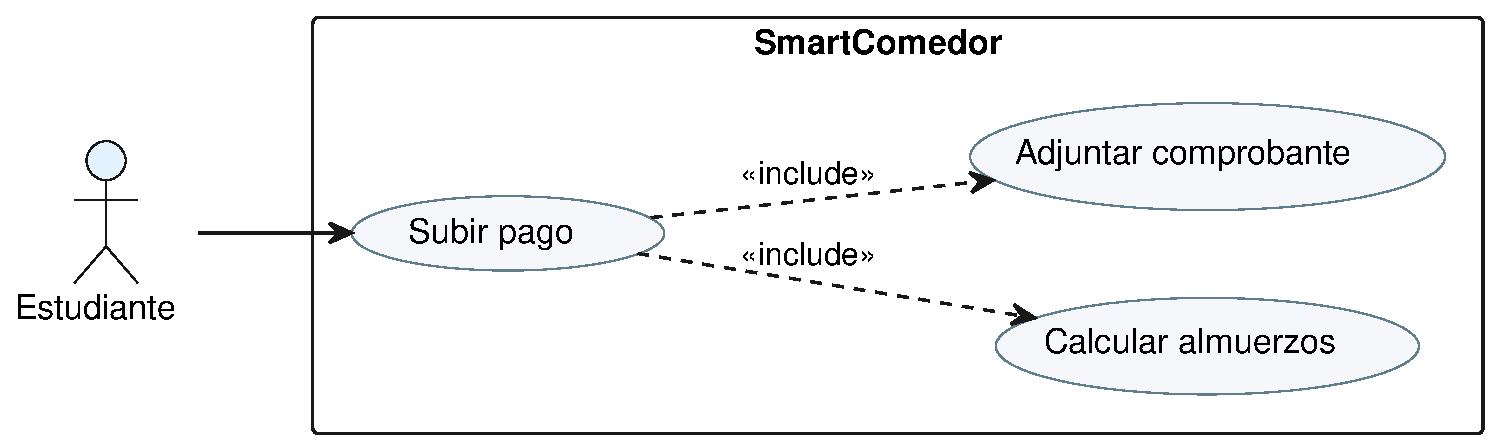
\includegraphics[width=\linewidth,height=0.30\textheight,keepaspectratio]{cu/cu11-uc.pdf}\caption{Diagrama de caso de uso --- CU-11}\end{figure}
\begin{figure}[H]\centering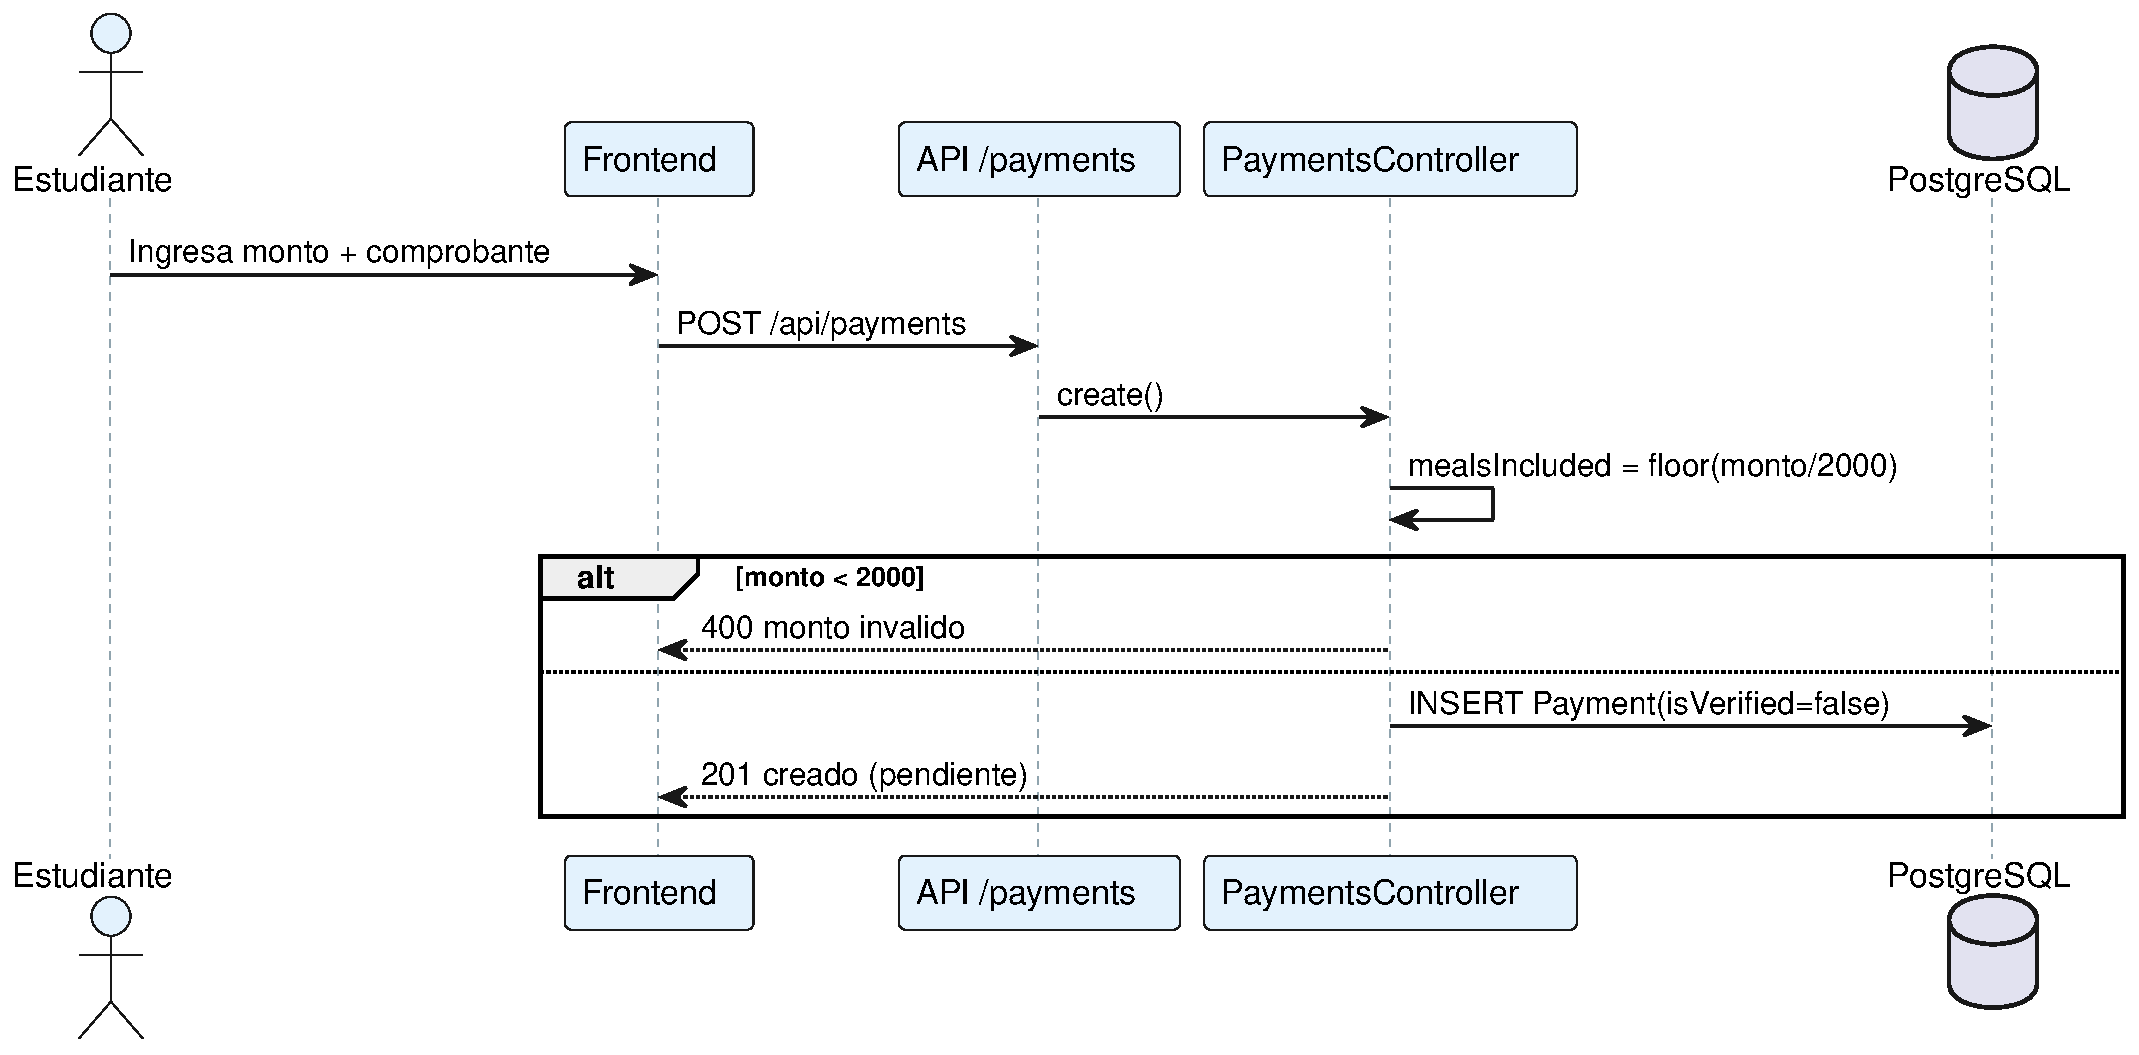
\includegraphics[width=\linewidth,height=0.42\textheight,keepaspectratio]{cu/cu11-seq.pdf}\caption{Diagrama de secuencia --- CU-11}\end{figure}
\begin{figure}[H]\centering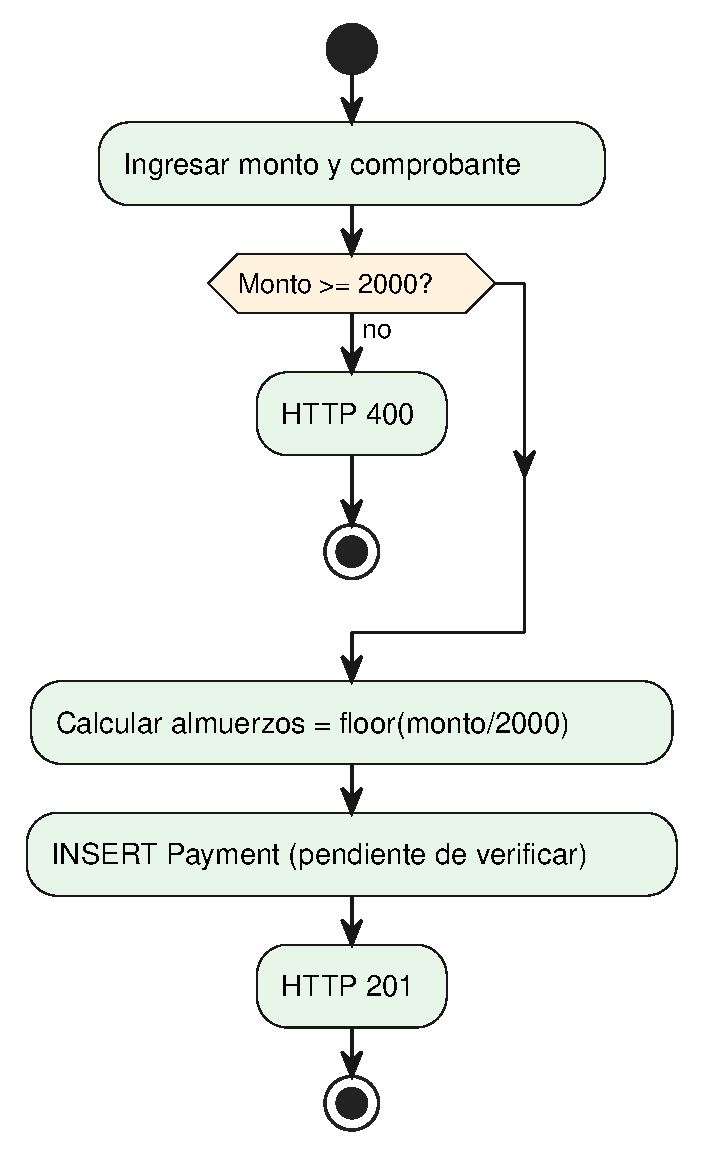
\includegraphics[width=\linewidth,height=0.46\textheight,keepaspectratio]{cu/cu11-act.pdf}\caption{Diagrama de actividades --- CU-11}\end{figure}

\subsection{CU-12 --- Verificar pago}

\noindent\textbf{Endpoint(s):} \texttt{PATCH /api/payments/:id/verify}\par\vspace{4pt}

\begin{table}[H]\centering\small
\caption{Ficha del caso de uso CU-12 --- Verificar pago}
\begin{tabularx}{\textwidth}{L{0.26\textwidth} X}
\toprule
\textbf{Campo} & \textbf{Descripcion} \\ \midrule
Objetivo del contexto & Permitir al administrador verificar un pago para habilitar los almuerzos del estudiante, dejando trazabilidad. \\ \midrule
Precondiciones & El pago debe existir y estar pendiente. \\ \midrule
Condicion de exito & El pago queda verificado y se registra en auditoria. \\ \midrule
Condicion de fracaso & El pago no existe. \\ \midrule
Actores principales & Administrador \\ \midrule
Actores secundarios & Servicio de auditoria \\
\bottomrule\end{tabularx}\end{table}
\begin{table}[H]\centering\small
\caption{Flujo principal de CU-12}
\begin{tabularx}{\textwidth}{C{0.10\textwidth} X}
\toprule \textbf{Paso} & \textbf{Accion} \\ \midrule
1 & El administrador selecciona el pago a verificar. \\
2 & El sistema verifica que el pago exista. \\
3 & El sistema marca isVerified=true (verifiedBy, verifiedAt). \\
4 & El sistema registra el evento en auditoria. \\
5 & El sistema responde 200. \\
\bottomrule\end{tabularx}\end{table}
\begin{table}[H]\centering\small
\caption{Extensiones (flujos alternativos) de CU-12}
\begin{tabularx}{\textwidth}{C{0.10\textwidth} X}
\toprule \textbf{Paso} & \textbf{Accion} \\ \midrule
2.1 & Pago inexistente $\rightarrow$ HTTP 404. \\
\bottomrule\end{tabularx}\end{table}
\begin{figure}[H]\centering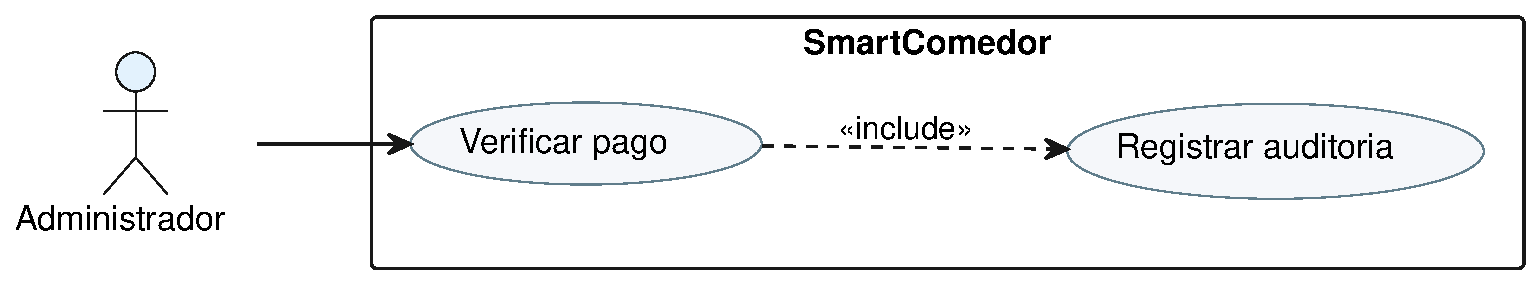
\includegraphics[width=\linewidth,height=0.30\textheight,keepaspectratio]{cu/cu12-uc.pdf}\caption{Diagrama de caso de uso --- CU-12}\end{figure}
\begin{figure}[H]\centering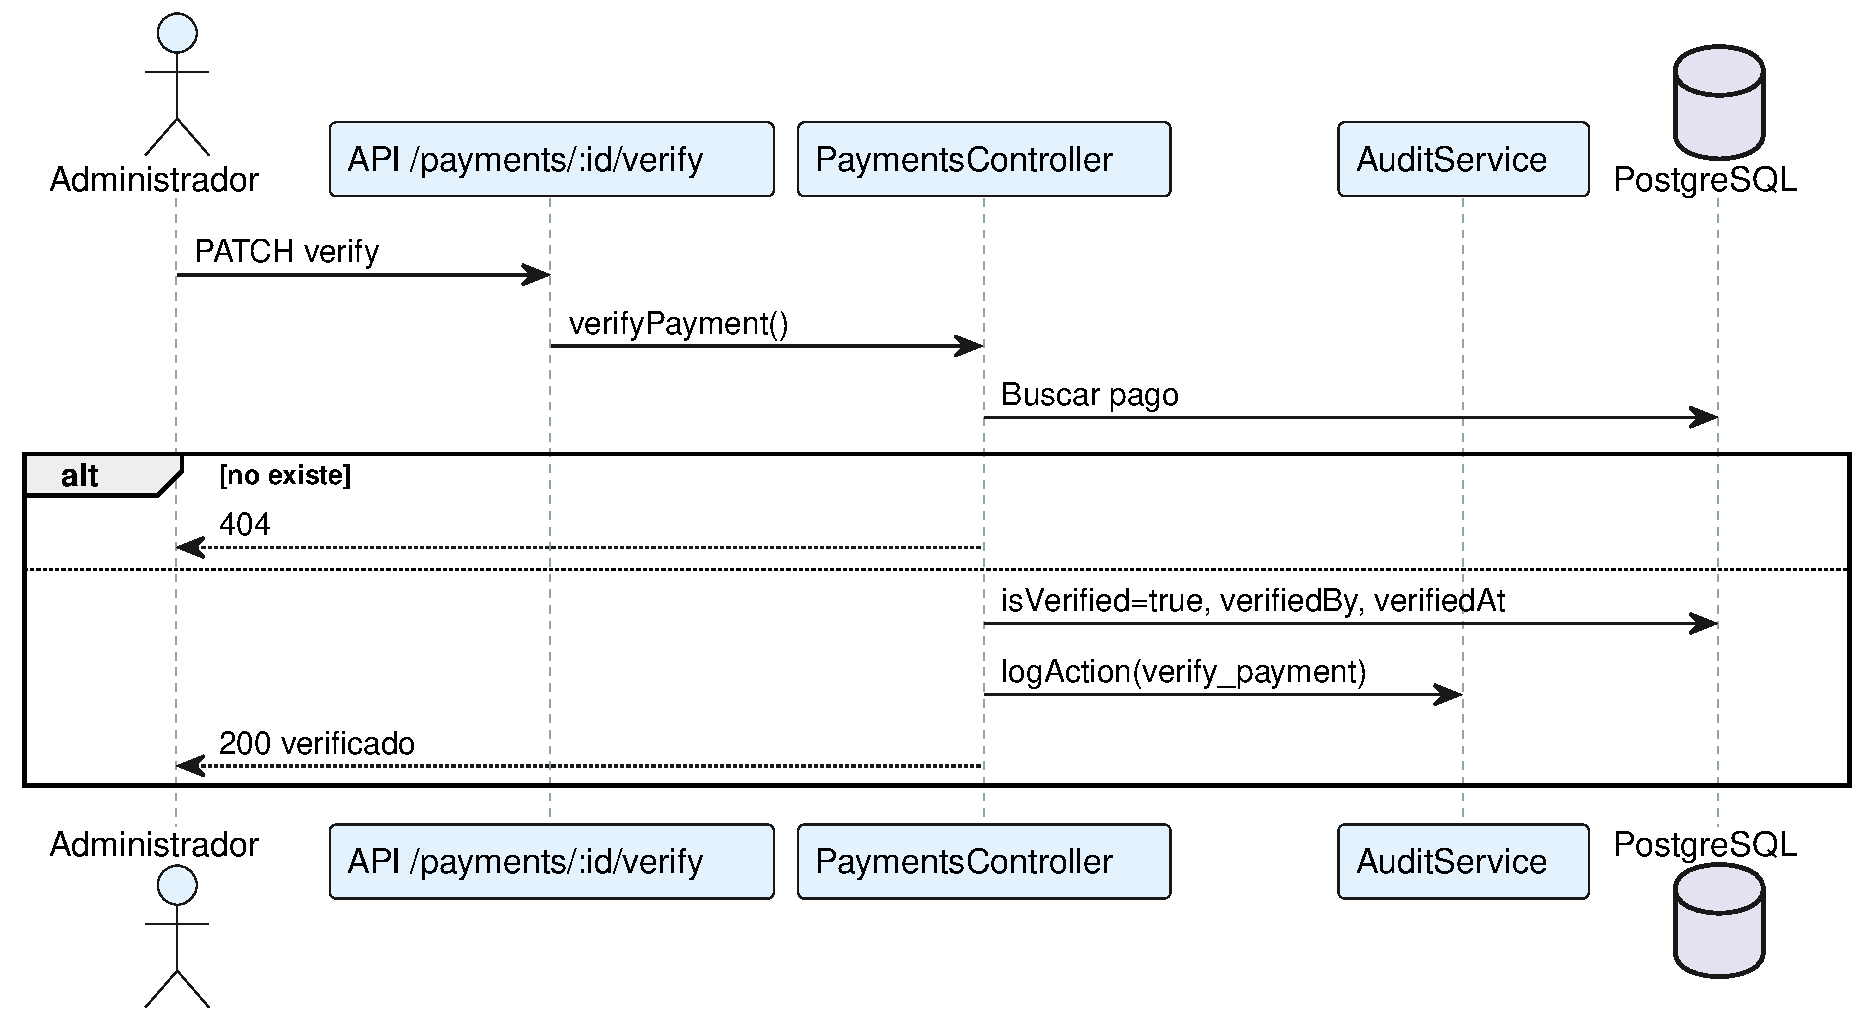
\includegraphics[width=\linewidth,height=0.42\textheight,keepaspectratio]{cu/cu12-seq.pdf}\caption{Diagrama de secuencia --- CU-12}\end{figure}
\begin{figure}[H]\centering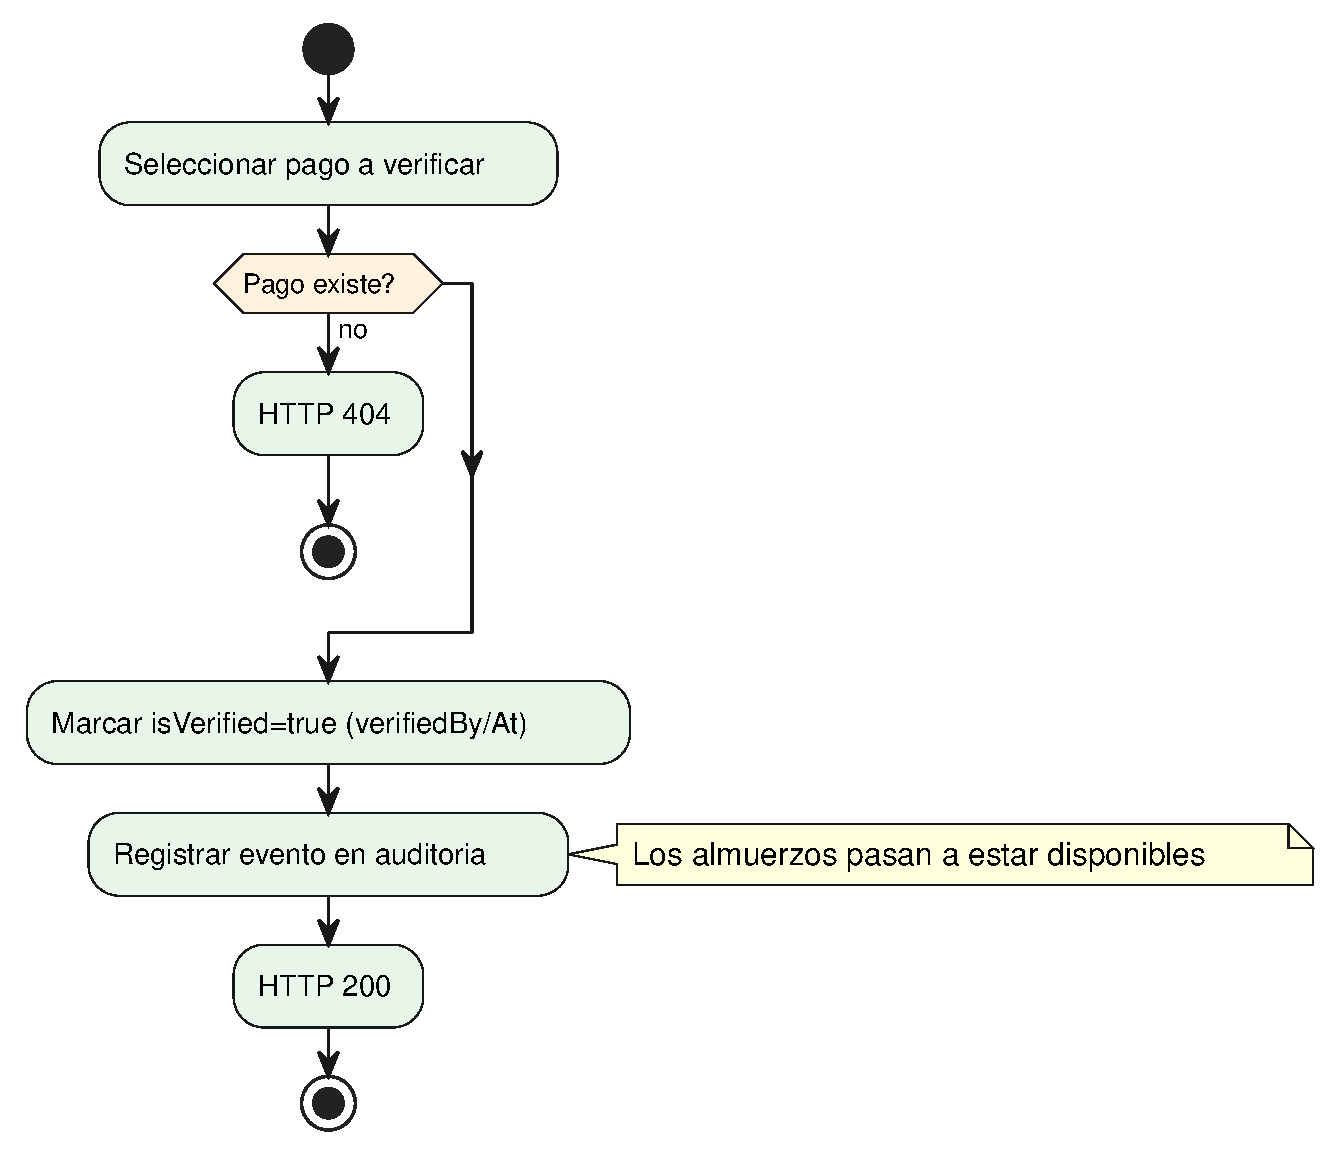
\includegraphics[width=\linewidth,height=0.46\textheight,keepaspectratio]{cu/cu12-act.pdf}\caption{Diagrama de actividades --- CU-12}\end{figure}

\subsection{CU-13 --- Calcular almuerzos por monto}

\noindent\textbf{Endpoint(s):} \texttt{POST /api/payments/calculate}\par\vspace{4pt}

\begin{table}[H]\centering\small
\caption{Ficha del caso de uso CU-13 --- Calcular almuerzos por monto}
\begin{tabularx}{\textwidth}{L{0.26\textwidth} X}
\toprule
\textbf{Campo} & \textbf{Descripcion} \\ \midrule
Objetivo del contexto & Permitir a un usuario autenticado conocer cuantos almuerzos corresponden a un monto dado, antes de registrar el pago. \\ \midrule
Precondiciones & El usuario debe estar autenticado. \\ \midrule
Condicion de exito & Se devuelve el numero de almuerzos y el residuo. \\ \midrule
Condicion de fracaso & El monto es invalido. \\ \midrule
Actores principales & Usuario autenticado \\ \midrule
Actores secundarios & - \\
\bottomrule\end{tabularx}\end{table}
\begin{table}[H]\centering\small
\caption{Flujo principal de CU-13}
\begin{tabularx}{\textwidth}{C{0.10\textwidth} X}
\toprule \textbf{Paso} & \textbf{Accion} \\ \midrule
1 & El usuario envia un monto. \\
2 & El sistema valida que el monto sea mayor o igual a 2000. \\
3 & El sistema calcula almuerzos=piso(monto/2000) y el residuo. \\
4 & El sistema responde 200 con el resultado. \\
\bottomrule\end{tabularx}\end{table}
\begin{table}[H]\centering\small
\caption{Extensiones (flujos alternativos) de CU-13}
\begin{tabularx}{\textwidth}{C{0.10\textwidth} X}
\toprule \textbf{Paso} & \textbf{Accion} \\ \midrule
2.1 & Monto menor a 2000 o no numerico $\rightarrow$ HTTP 400. \\
\bottomrule\end{tabularx}\end{table}
\begin{figure}[H]\centering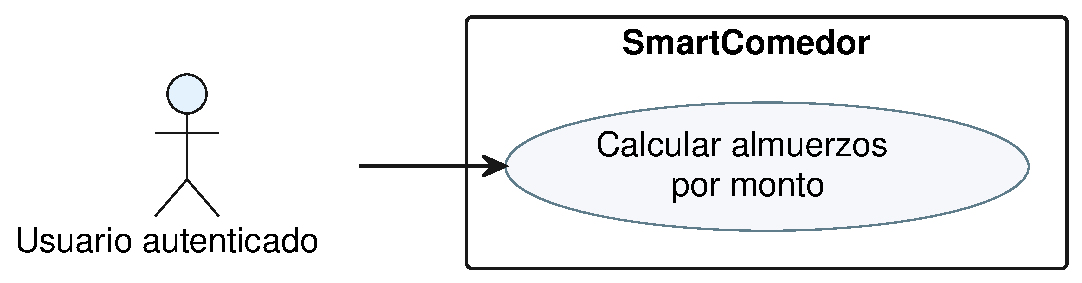
\includegraphics[width=\linewidth,height=0.30\textheight,keepaspectratio]{cu/cu13-uc.pdf}\caption{Diagrama de caso de uso --- CU-13}\end{figure}
\begin{figure}[H]\centering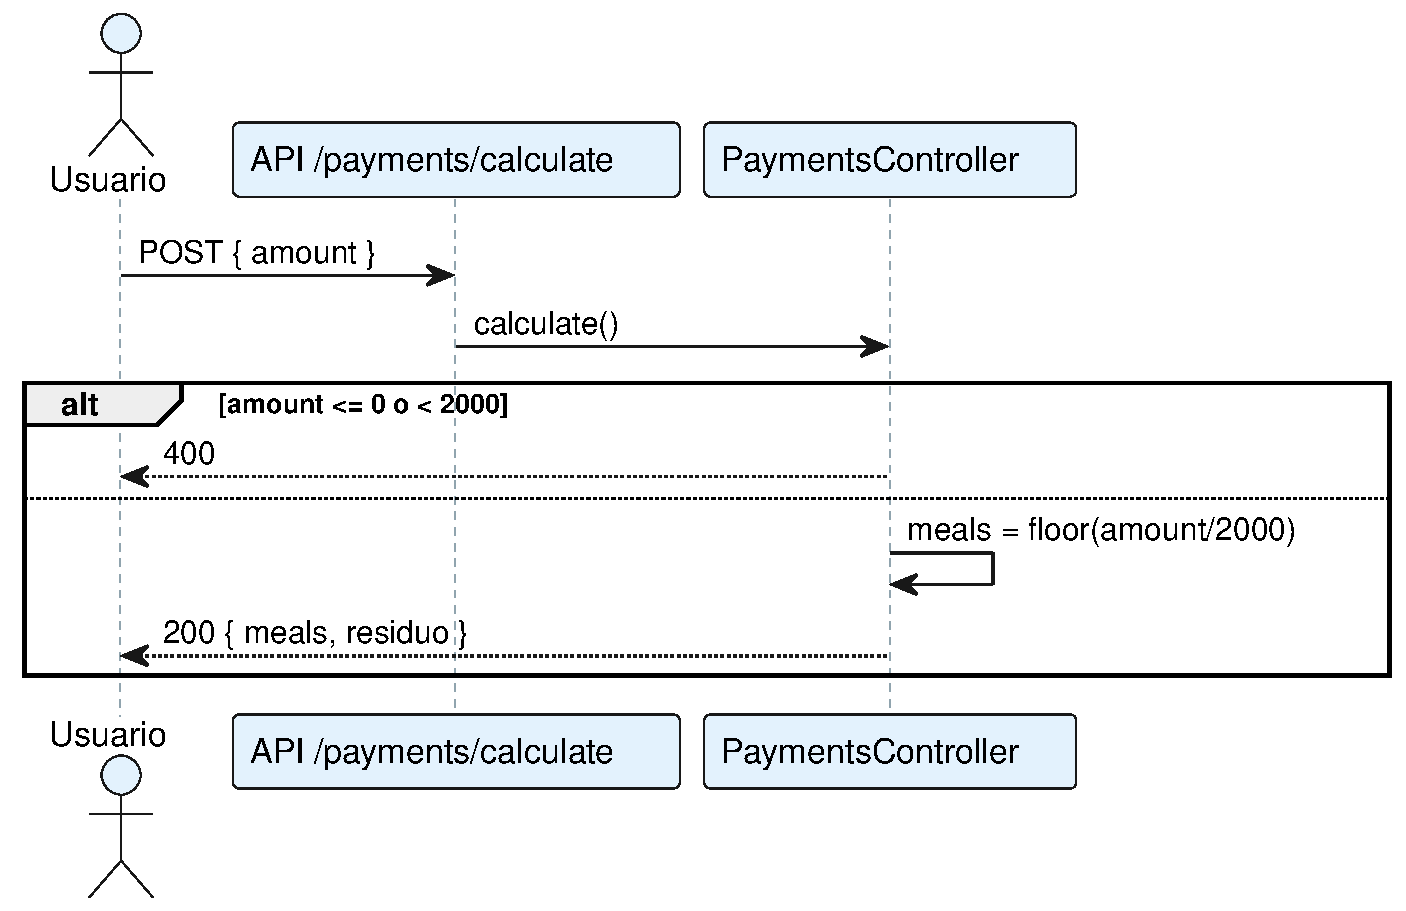
\includegraphics[width=\linewidth,height=0.42\textheight,keepaspectratio]{cu/cu13-seq.pdf}\caption{Diagrama de secuencia --- CU-13}\end{figure}
\begin{figure}[H]\centering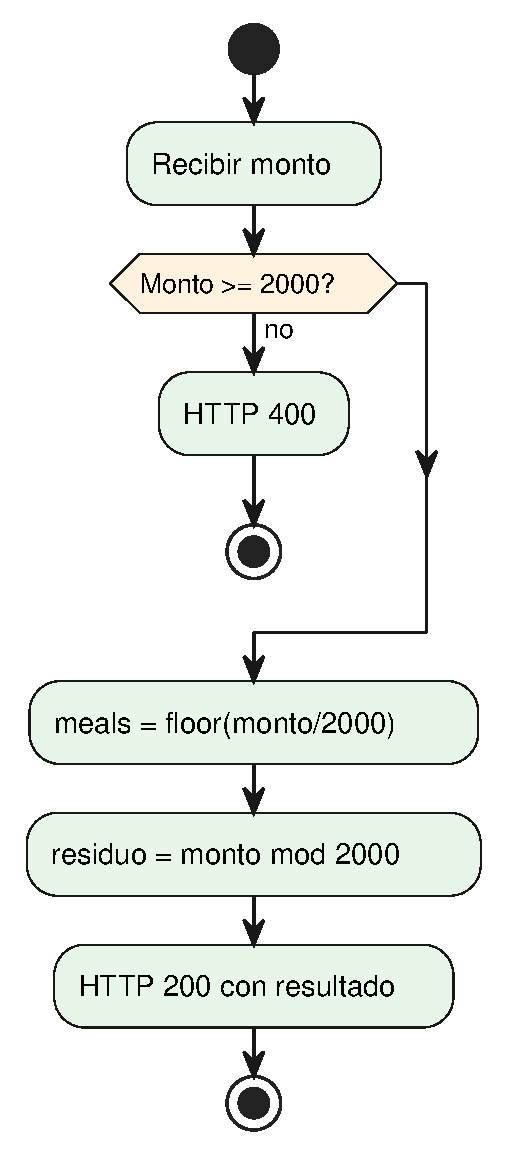
\includegraphics[width=\linewidth,height=0.46\textheight,keepaspectratio]{cu/cu13-act.pdf}\caption{Diagrama de actividades --- CU-13}\end{figure}

\subsection{CU-14 --- Registrar almuerzo}

\noindent\textbf{Endpoint(s):} \texttt{POST /api/meals}\par\vspace{4pt}

\begin{table}[H]\centering\small
\caption{Ficha del caso de uso CU-14 --- Registrar almuerzo}
\begin{tabularx}{\textwidth}{L{0.26\textwidth} X}
\toprule
\textbf{Campo} & \textbf{Descripcion} \\ \midrule
Objetivo del contexto & Permitir al supervisor registrar el consumo de almuerzo de un estudiante validando todas las reglas de elegibilidad del dia. \\ \midrule
Precondiciones & El supervisor debe estar autenticado; el estudiante debe estar activo y tener almuerzos. \\ \midrule
Condicion de exito & Se registra la asistencia, se descuenta un almuerzo y se deja bitacora. \\ \midrule
Condicion de fracaso & El estudiante no cumple alguna regla (inactivo, dia no permitido, ya comio, sin saldo). \\ \midrule
Actores principales & Supervisor \\ \midrule
Actores secundarios & Servicios de bitacora y auditoria \\
\bottomrule\end{tabularx}\end{table}
\begin{table}[H]\centering\small
\caption{Flujo principal de CU-14}
\begin{tabularx}{\textwidth}{C{0.10\textwidth} X}
\toprule \textbf{Paso} & \textbf{Accion} \\ \midrule
1 & El supervisor busca al estudiante por QR, cedula o UID. \\
2 & El sistema valida que exista y este activo. \\
3 & El sistema valida el dia autorizado y que no haya comido hoy. \\
4 & El sistema valida que tenga almuerzos disponibles. \\
5 & El sistema registra la asistencia e incrementa mealsUsed. \\
6 & El sistema registra la bitacora y la auditoria, y responde 201. \\
\bottomrule\end{tabularx}\end{table}
\begin{table}[H]\centering\small
\caption{Extensiones (flujos alternativos) de CU-14}
\begin{tabularx}{\textwidth}{C{0.10\textwidth} X}
\toprule \textbf{Paso} & \textbf{Accion} \\ \midrule
2.1 & Estudiante inexistente $\rightarrow$ 404; inactivo $\rightarrow$ 400. \\
3.1 & Dia no autorizado o ya comio hoy $\rightarrow$ 400. \\
4.1 & Sin almuerzos disponibles $\rightarrow$ 400. \\
\bottomrule\end{tabularx}\end{table}
\begin{figure}[H]\centering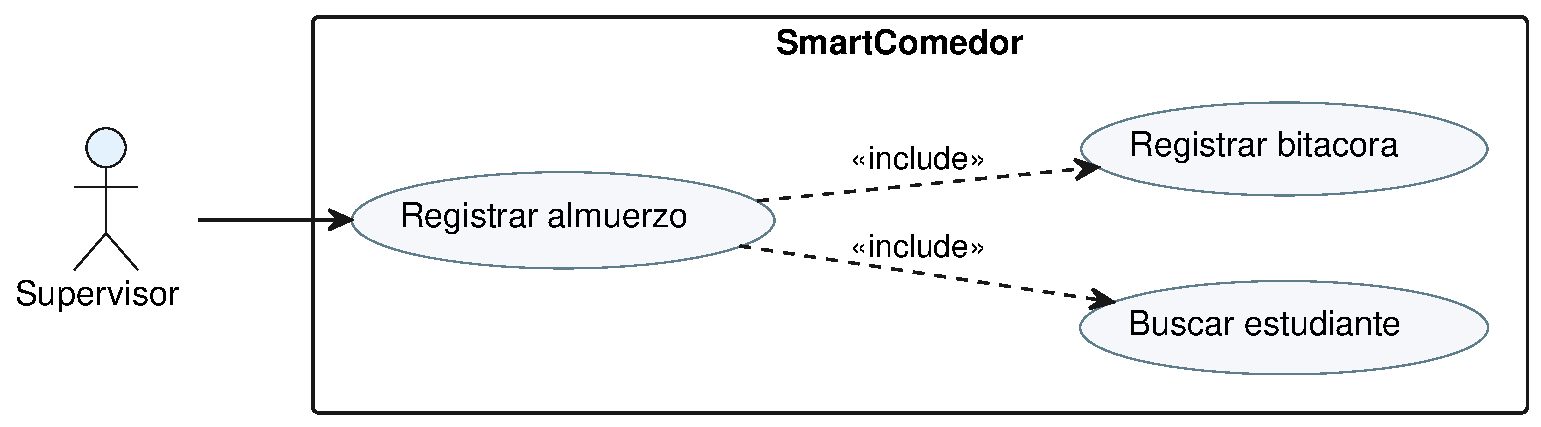
\includegraphics[width=\linewidth,height=0.30\textheight,keepaspectratio]{cu/cu14-uc.pdf}\caption{Diagrama de caso de uso --- CU-14}\end{figure}
\begin{figure}[H]\centering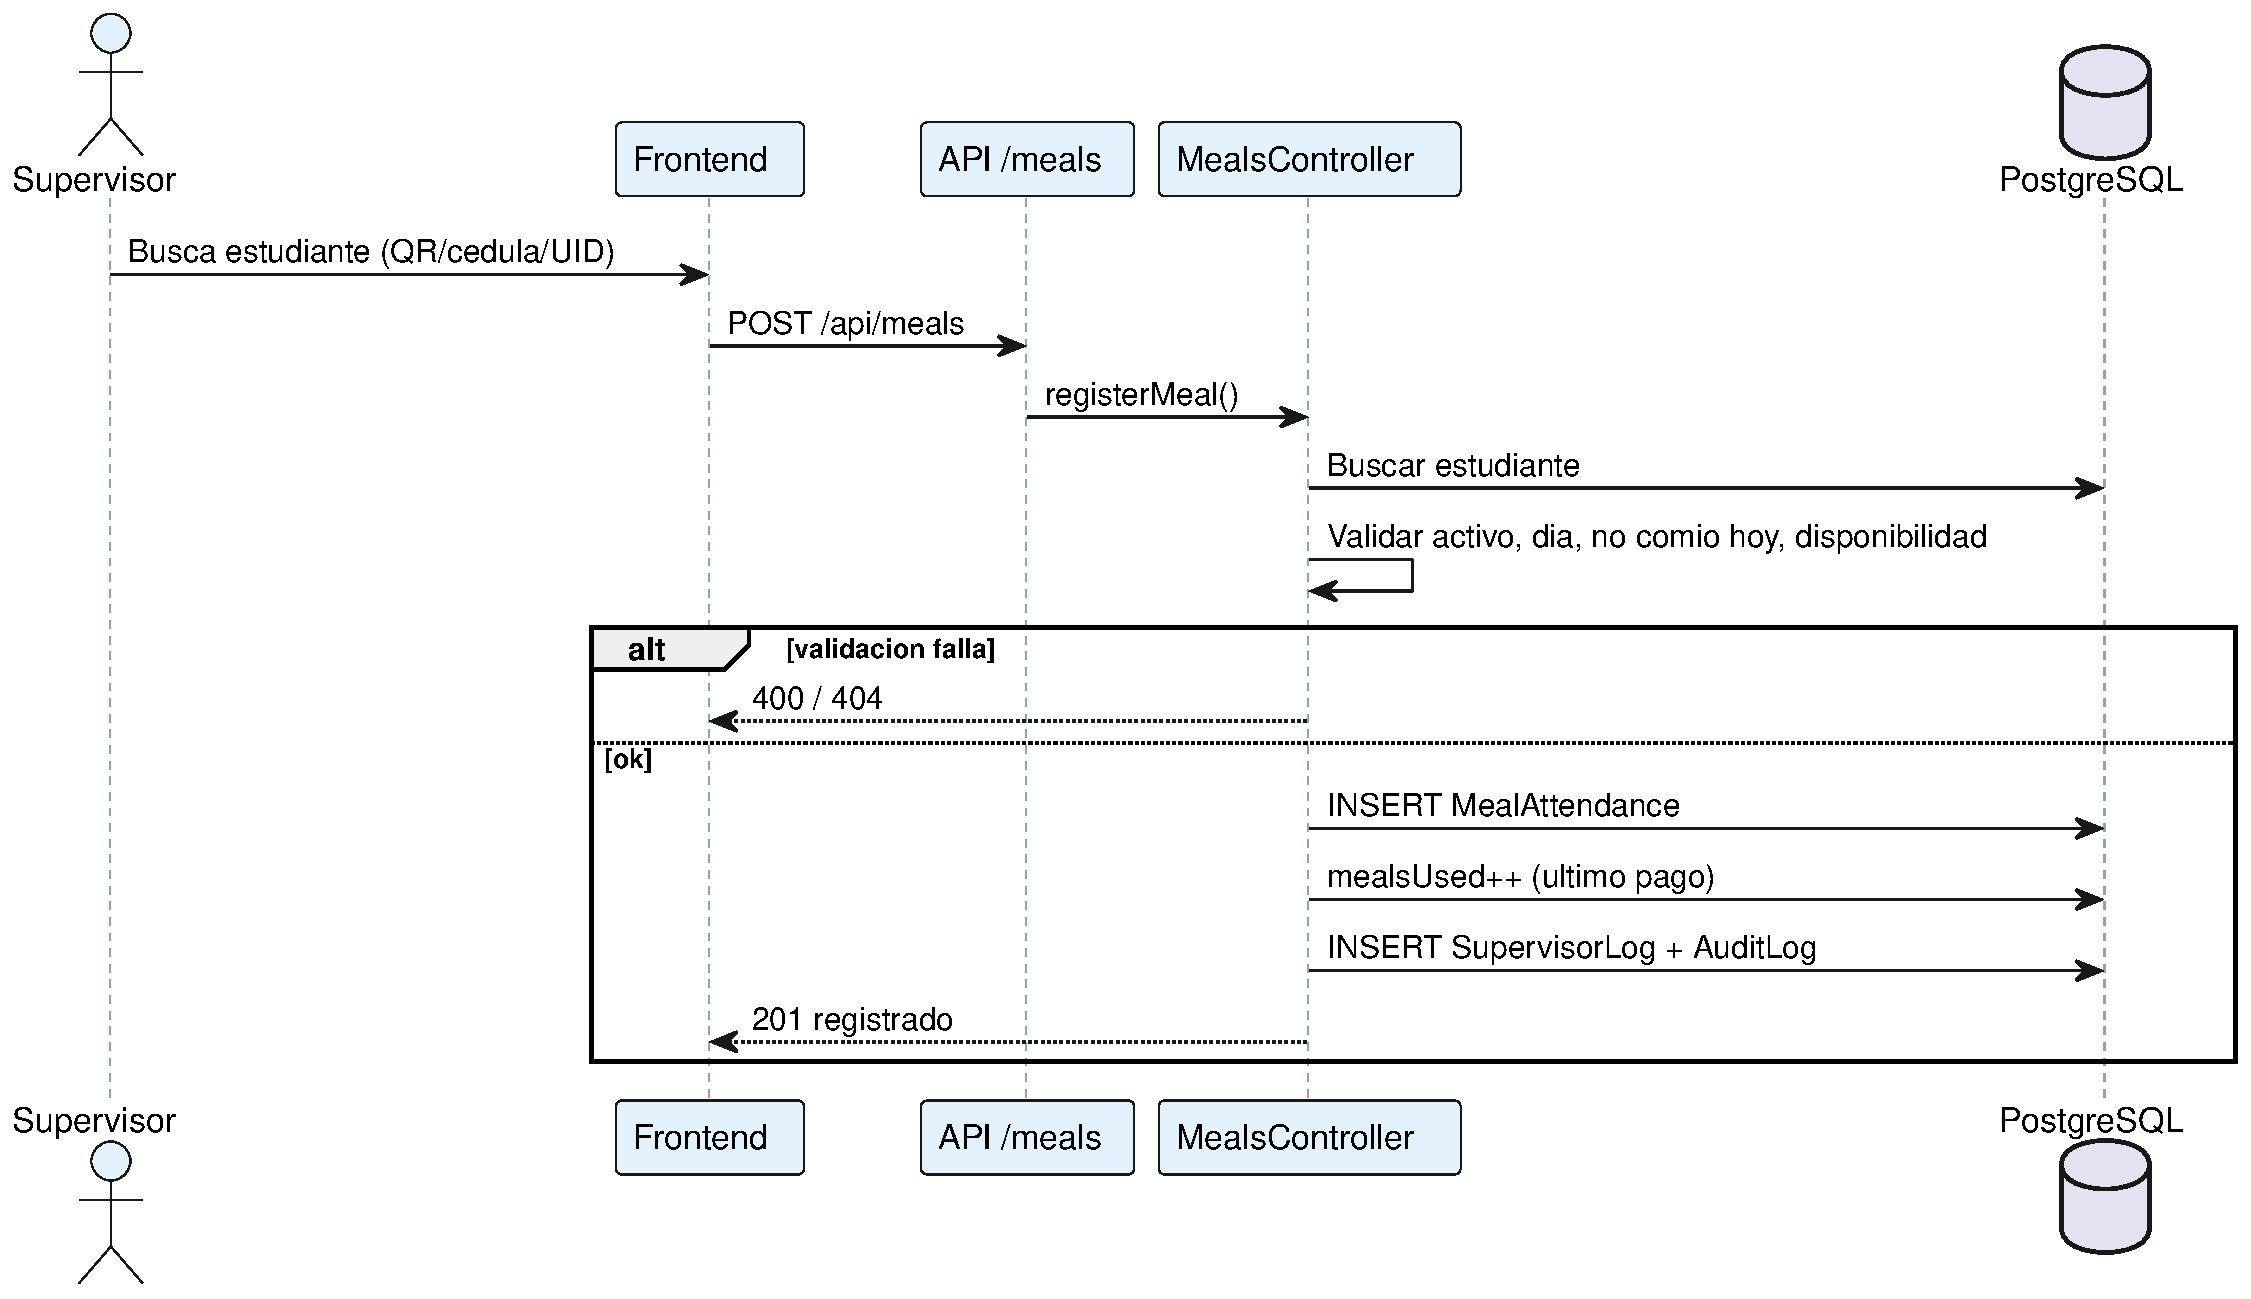
\includegraphics[width=\linewidth,height=0.42\textheight,keepaspectratio]{cu/cu14-seq.pdf}\caption{Diagrama de secuencia --- CU-14}\end{figure}
\begin{figure}[H]\centering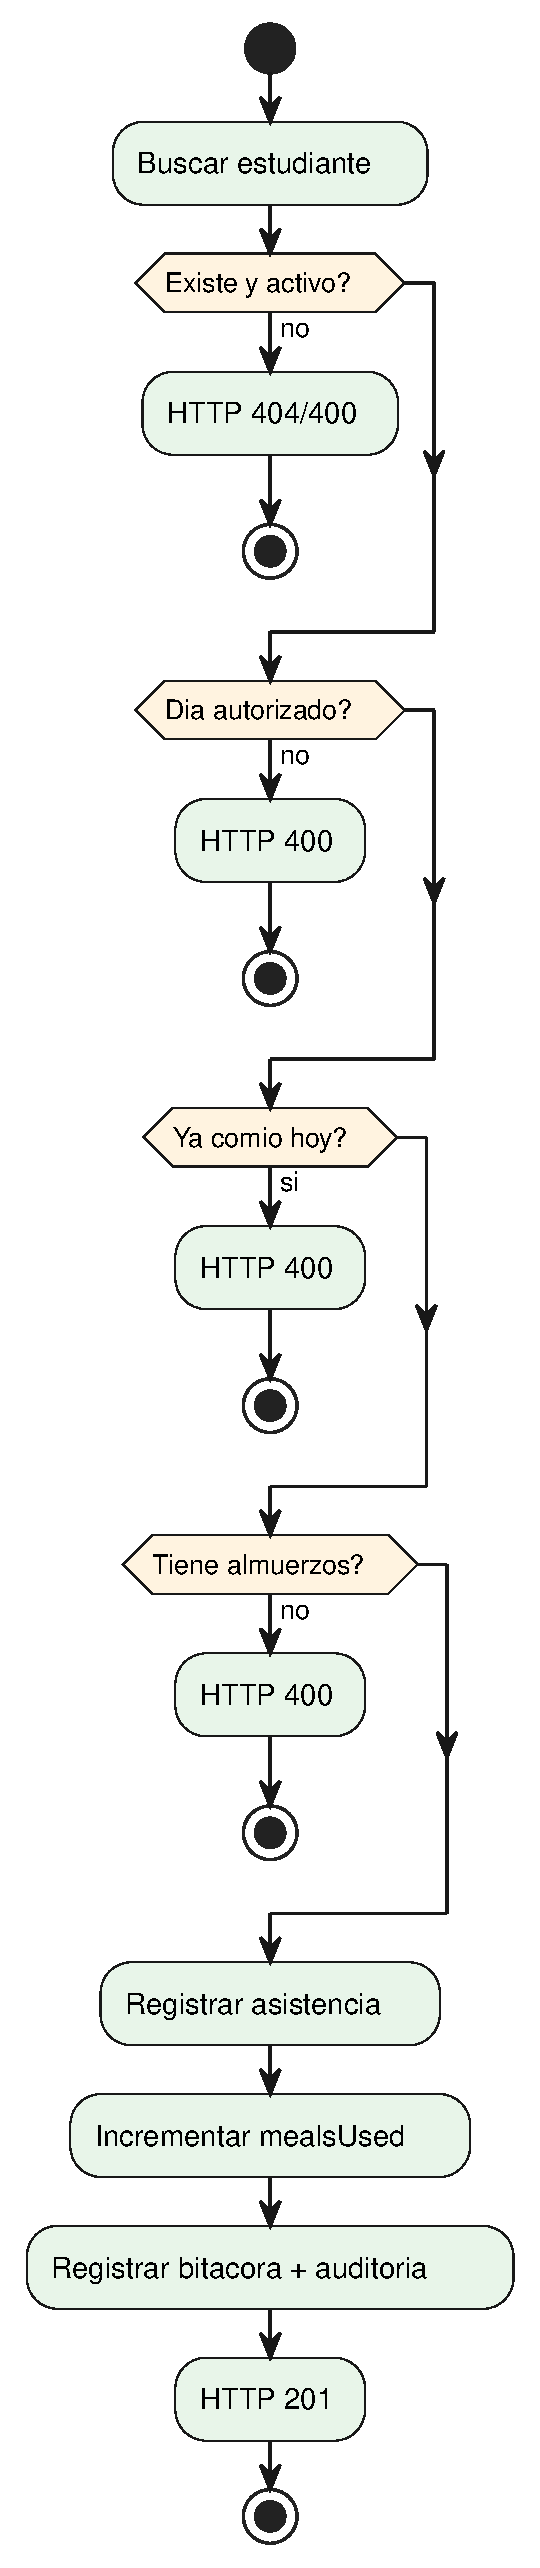
\includegraphics[width=\linewidth,height=0.46\textheight,keepaspectratio]{cu/cu14-act.pdf}\caption{Diagrama de actividades --- CU-14}\end{figure}

\subsection{CU-15 --- Consultar historial y asistencia del dia}

\noindent\textbf{Endpoint(s):} \texttt{GET /api/meals/history, GET /api/meals/today}\par\vspace{4pt}

\begin{table}[H]\centering\small
\caption{Ficha del caso de uso CU-15 --- Consultar historial y asistencia del dia}
\begin{tabularx}{\textwidth}{L{0.26\textwidth} X}
\toprule
\textbf{Campo} & \textbf{Descripcion} \\ \midrule
Objetivo del contexto & Permitir a los usuarios autorizados consultar el historial de almuerzos y la asistencia del dia. \\ \midrule
Precondiciones & El usuario debe estar autenticado. \\ \midrule
Condicion de exito & Se devuelven los registros segun los filtros. \\ \midrule
Condicion de fracaso & Parametros de filtro invalidos. \\ \midrule
Actores principales & Usuario autenticado \\ \midrule
Actores secundarios & Base de datos \\
\bottomrule\end{tabularx}\end{table}
\begin{table}[H]\centering\small
\caption{Flujo principal de CU-15}
\begin{tabularx}{\textwidth}{C{0.10\textwidth} X}
\toprule \textbf{Paso} & \textbf{Accion} \\ \midrule
1 & El usuario elige consultar historial o asistencia del dia. \\
2 & El usuario aplica filtros (estudiante, rango de fechas). \\
3 & El sistema consulta las asistencias correspondientes. \\
4 & El sistema responde 200 con los resultados. \\
\bottomrule\end{tabularx}\end{table}
\begin{table}[H]\centering\small
\caption{Extensiones (flujos alternativos) de CU-15}
\begin{tabularx}{\textwidth}{C{0.10\textwidth} X}
\toprule \textbf{Paso} & \textbf{Accion} \\ \midrule
2.1 & Filtros invalidos $\rightarrow$ HTTP 400. \\
\bottomrule\end{tabularx}\end{table}
\begin{figure}[H]\centering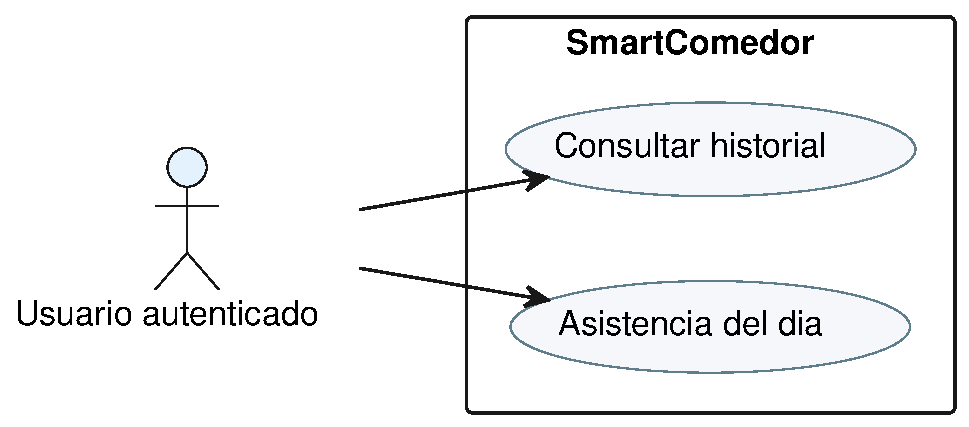
\includegraphics[width=\linewidth,height=0.30\textheight,keepaspectratio]{cu/cu15-uc.pdf}\caption{Diagrama de caso de uso --- CU-15}\end{figure}
\begin{figure}[H]\centering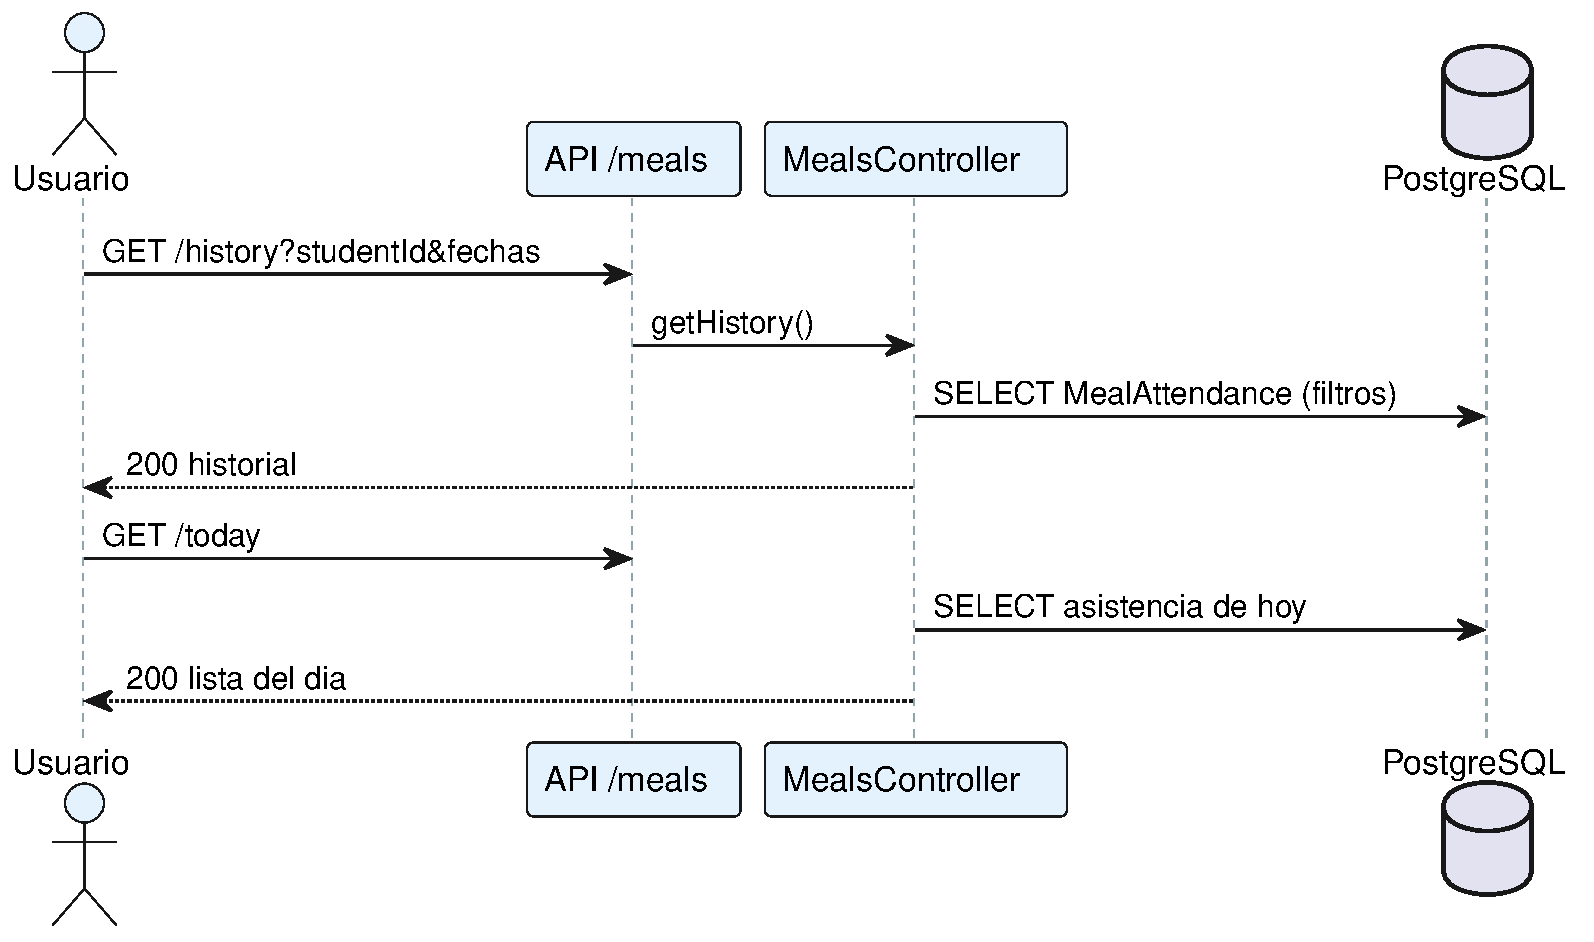
\includegraphics[width=\linewidth,height=0.42\textheight,keepaspectratio]{cu/cu15-seq.pdf}\caption{Diagrama de secuencia --- CU-15}\end{figure}
\begin{figure}[H]\centering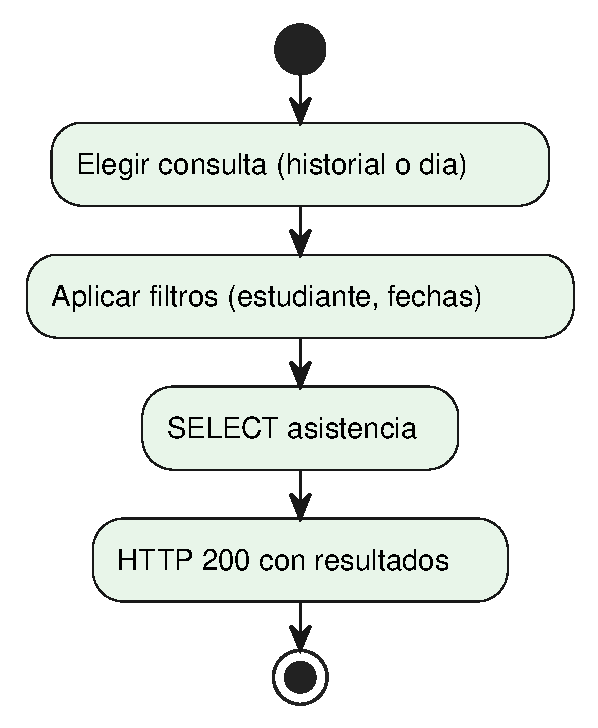
\includegraphics[width=\linewidth,height=0.46\textheight,keepaspectratio]{cu/cu15-act.pdf}\caption{Diagrama de actividades --- CU-15}\end{figure}

\subsection{CU-16 --- Consultar analitica del tablero}

\noindent\textbf{Endpoint(s):} \texttt{GET /api/meals/analytics}\par\vspace{4pt}

\begin{table}[H]\centering\small
\caption{Ficha del caso de uso CU-16 --- Consultar analitica del tablero}
\begin{tabularx}{\textwidth}{L{0.26\textwidth} X}
\toprule
\textbf{Campo} & \textbf{Descripcion} \\ \midrule
Objetivo del contexto & Proveer indicadores agregados (KPIs) del servicio de comedor para la toma de decisiones. \\ \midrule
Precondiciones & El usuario debe tener rol admin o auditor. \\ \midrule
Condicion de exito & Se devuelven las metricas agregadas. \\ \midrule
Condicion de fracaso & Sin autorizacion. \\ \midrule
Actores principales & Administrador, Auditor externo \\ \midrule
Actores secundarios & Base de datos \\
\bottomrule\end{tabularx}\end{table}
\begin{table}[H]\centering\small
\caption{Flujo principal de CU-16}
\begin{tabularx}{\textwidth}{C{0.10\textwidth} X}
\toprule \textbf{Paso} & \textbf{Accion} \\ \midrule
1 & El usuario solicita la analitica del tablero. \\
2 & El sistema ejecuta las agregaciones (conteos y totales). \\
3 & El sistema construye la respuesta con los KPIs. \\
4 & El sistema responde 200. \\
\bottomrule\end{tabularx}\end{table}
\begin{table}[H]\centering\small
\caption{Extensiones (flujos alternativos) de CU-16}
\begin{tabularx}{\textwidth}{C{0.10\textwidth} X}
\toprule \textbf{Paso} & \textbf{Accion} \\ \midrule
1.1 & Rol no autorizado $\rightarrow$ HTTP 403. \\
\bottomrule\end{tabularx}\end{table}
\begin{figure}[H]\centering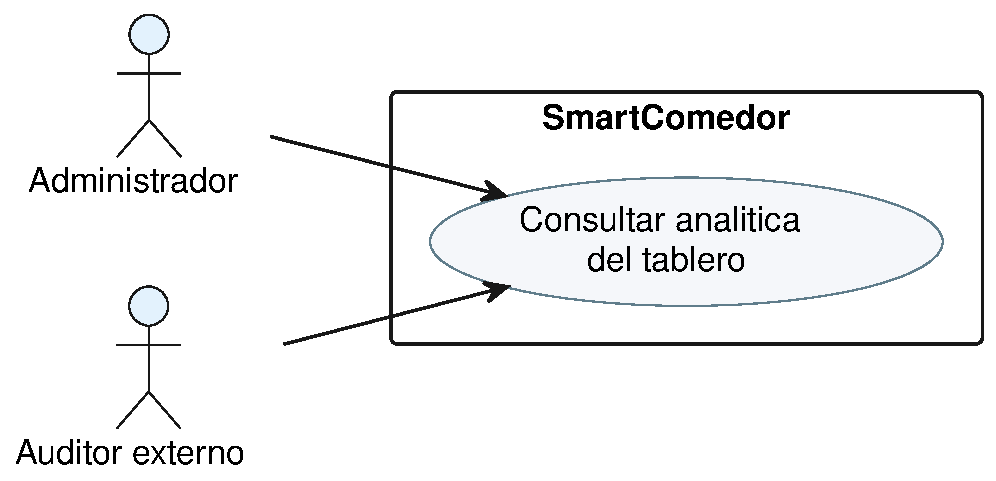
\includegraphics[width=\linewidth,height=0.30\textheight,keepaspectratio]{cu/cu16-uc.pdf}\caption{Diagrama de caso de uso --- CU-16}\end{figure}
\begin{figure}[H]\centering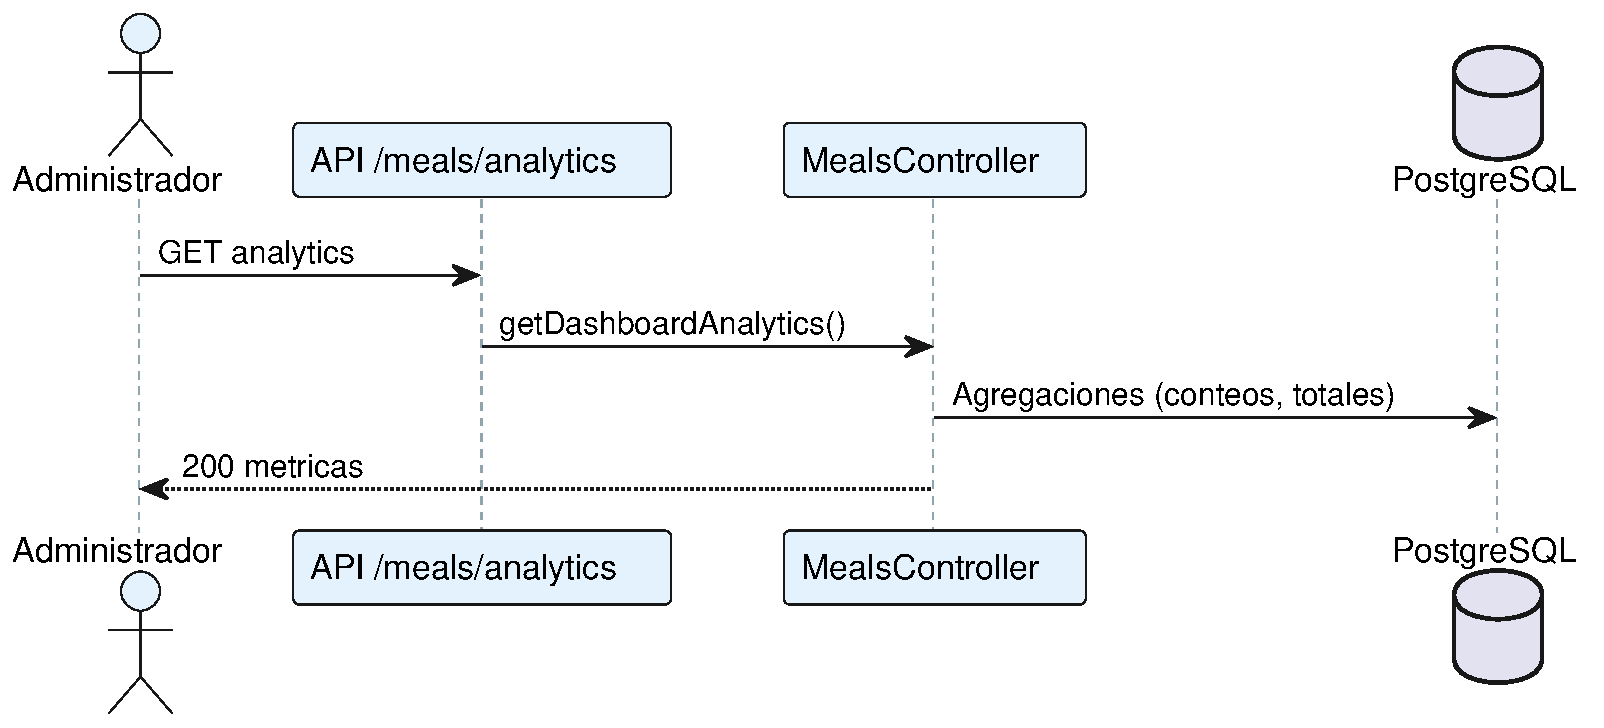
\includegraphics[width=\linewidth,height=0.42\textheight,keepaspectratio]{cu/cu16-seq.pdf}\caption{Diagrama de secuencia --- CU-16}\end{figure}
\begin{figure}[H]\centering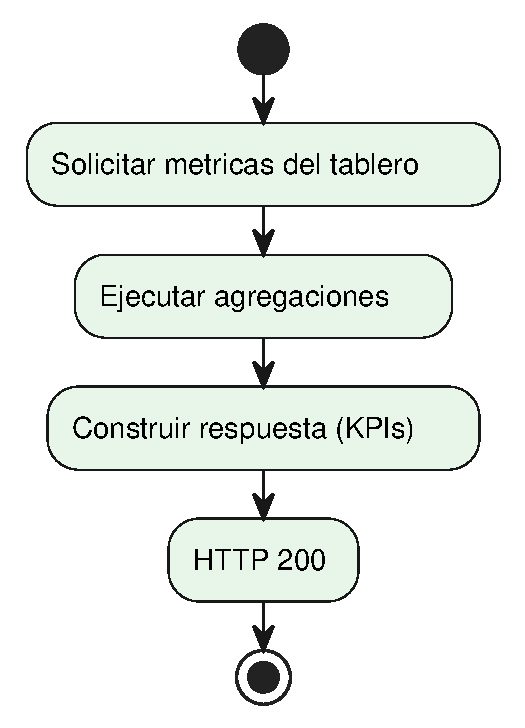
\includegraphics[width=\linewidth,height=0.46\textheight,keepaspectratio]{cu/cu16-act.pdf}\caption{Diagrama de actividades --- CU-16}\end{figure}

\subsection{CU-17 --- Gestionar ciclos y cierre automatico}

\noindent\textbf{Endpoint(s):} \texttt{GET/POST/PUT /api/cycles + tarea programada}\par\vspace{4pt}

\begin{table}[H]\centering\small
\caption{Ficha del caso de uso CU-17 --- Gestionar ciclos y cierre automatico}
\begin{tabularx}{\textwidth}{L{0.26\textwidth} X}
\toprule
\textbf{Campo} & \textbf{Descripcion} \\ \midrule
Objetivo del contexto & Administrar los periodos del servicio y cerrar automaticamente los ciclos vencidos solicitando revalidacion documental. \\ \midrule
Precondiciones & Debe existir al menos un ciclo configurado. \\ \midrule
Condicion de exito & Los ciclos vencidos se cierran y los estudiantes quedan marcados para revalidacion. \\ \midrule
Condicion de fracaso & No hay ciclos vencidos por procesar. \\ \midrule
Actores principales & Administrador, Sistema (cron) \\ \midrule
Actores secundarios & Servicio de automatizacion de ciclos \\
\bottomrule\end{tabularx}\end{table}
\begin{table}[H]\centering\small
\caption{Flujo principal de CU-17}
\begin{tabularx}{\textwidth}{C{0.10\textwidth} X}
\toprule \textbf{Paso} & \textbf{Accion} \\ \midrule
1 & El administrador crea o cierra ciclos manualmente. \\
2 & Una tarea programada se ejecuta periodicamente. \\
3 & El sistema busca ciclos activos cuya fecha de fin ya paso. \\
4 & El sistema cierra cada ciclo y marca a los estudiantes para revalidacion. \\
\bottomrule\end{tabularx}\end{table}
\begin{table}[H]\centering\small
\caption{Extensiones (flujos alternativos) de CU-17}
\begin{tabularx}{\textwidth}{C{0.10\textwidth} X}
\toprule \textbf{Paso} & \textbf{Accion} \\ \midrule
3.1 & Si no hay ciclos vencidos, la tarea finaliza sin cambios. \\
\bottomrule\end{tabularx}\end{table}
\begin{figure}[H]\centering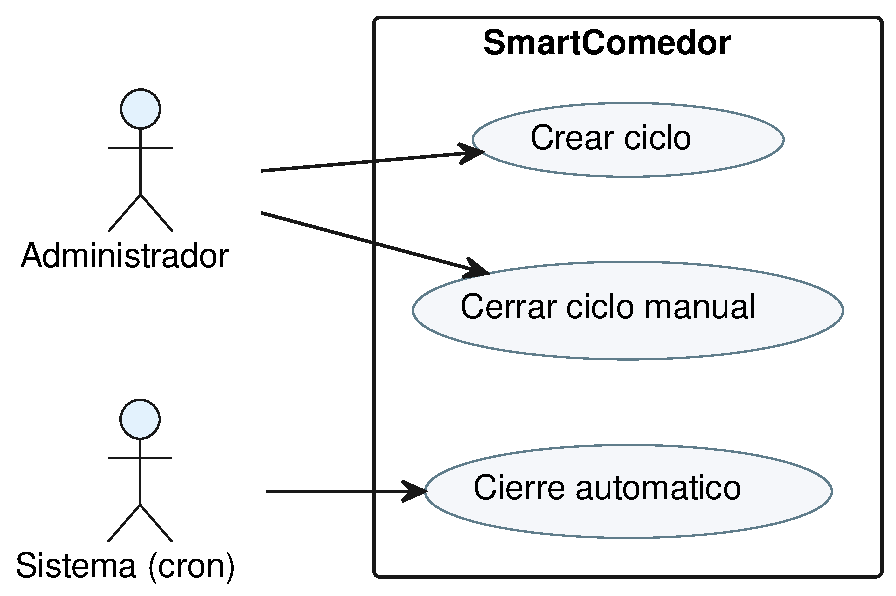
\includegraphics[width=\linewidth,height=0.30\textheight,keepaspectratio]{cu/cu17-uc.pdf}\caption{Diagrama de caso de uso --- CU-17}\end{figure}
\begin{figure}[H]\centering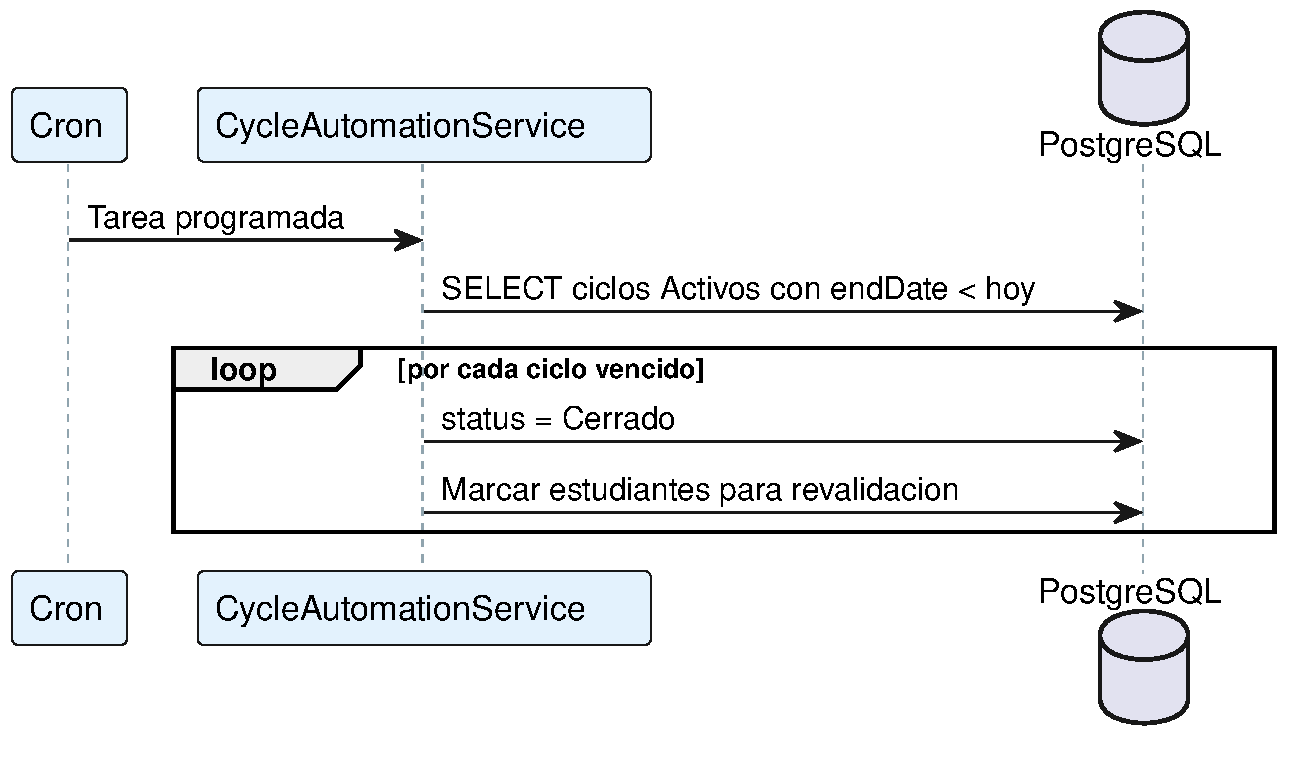
\includegraphics[width=\linewidth,height=0.42\textheight,keepaspectratio]{cu/cu17-seq.pdf}\caption{Diagrama de secuencia --- CU-17}\end{figure}
\begin{figure}[H]\centering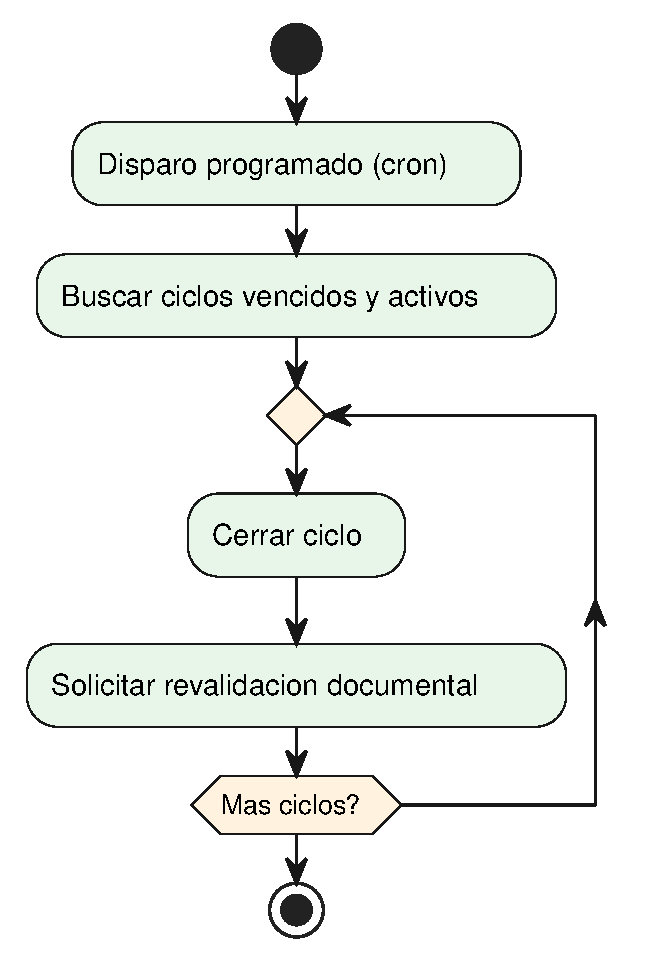
\includegraphics[width=\linewidth,height=0.46\textheight,keepaspectratio]{cu/cu17-act.pdf}\caption{Diagrama de actividades --- CU-17}\end{figure}

\subsection{CU-18 --- Calificar servicio}

\noindent\textbf{Endpoint(s):} \texttt{POST /api/ratings}\par\vspace{4pt}

\begin{table}[H]\centering\small
\caption{Ficha del caso de uso CU-18 --- Calificar servicio}
\begin{tabularx}{\textwidth}{L{0.26\textwidth} X}
\toprule
\textbf{Campo} & \textbf{Descripcion} \\ \midrule
Objetivo del contexto & Permitir al estudiante calificar el servicio del comedor con una puntuacion y un comentario opcional. \\ \midrule
Precondiciones & El estudiante debe estar autenticado. \\ \midrule
Condicion de exito & Se registra la calificacion y se actualiza el promedio. \\ \midrule
Condicion de fracaso & Usuario no autenticado. \\ \midrule
Actores principales & Estudiante \\ \midrule
Actores secundarios & Base de datos \\
\bottomrule\end{tabularx}\end{table}
\begin{table}[H]\centering\small
\caption{Flujo principal de CU-18}
\begin{tabularx}{\textwidth}{C{0.10\textwidth} X}
\toprule \textbf{Paso} & \textbf{Accion} \\ \midrule
1 & El estudiante selecciona una puntuacion de 1 a 5 estrellas. \\
2 & El estudiante agrega un comentario opcional. \\
3 & El sistema registra la calificacion. \\
4 & El sistema responde 201. \\
\bottomrule\end{tabularx}\end{table}
\begin{table}[H]\centering\small
\caption{Extensiones (flujos alternativos) de CU-18}
\begin{tabularx}{\textwidth}{C{0.10\textwidth} X}
\toprule \textbf{Paso} & \textbf{Accion} \\ \midrule
3.1 & Usuario no autenticado $\rightarrow$ HTTP 401. \\
\bottomrule\end{tabularx}\end{table}
\begin{figure}[H]\centering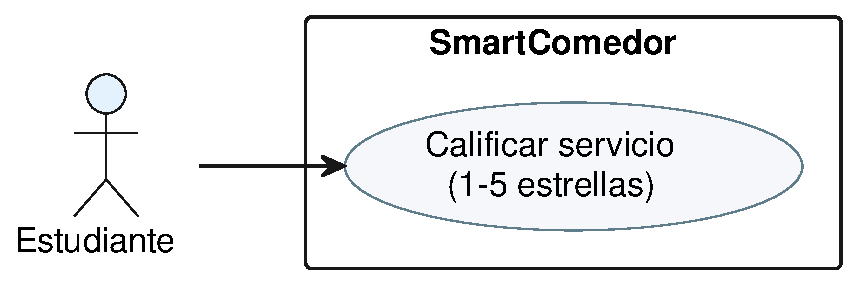
\includegraphics[width=\linewidth,height=0.30\textheight,keepaspectratio]{cu/cu18-uc.pdf}\caption{Diagrama de caso de uso --- CU-18}\end{figure}
\begin{figure}[H]\centering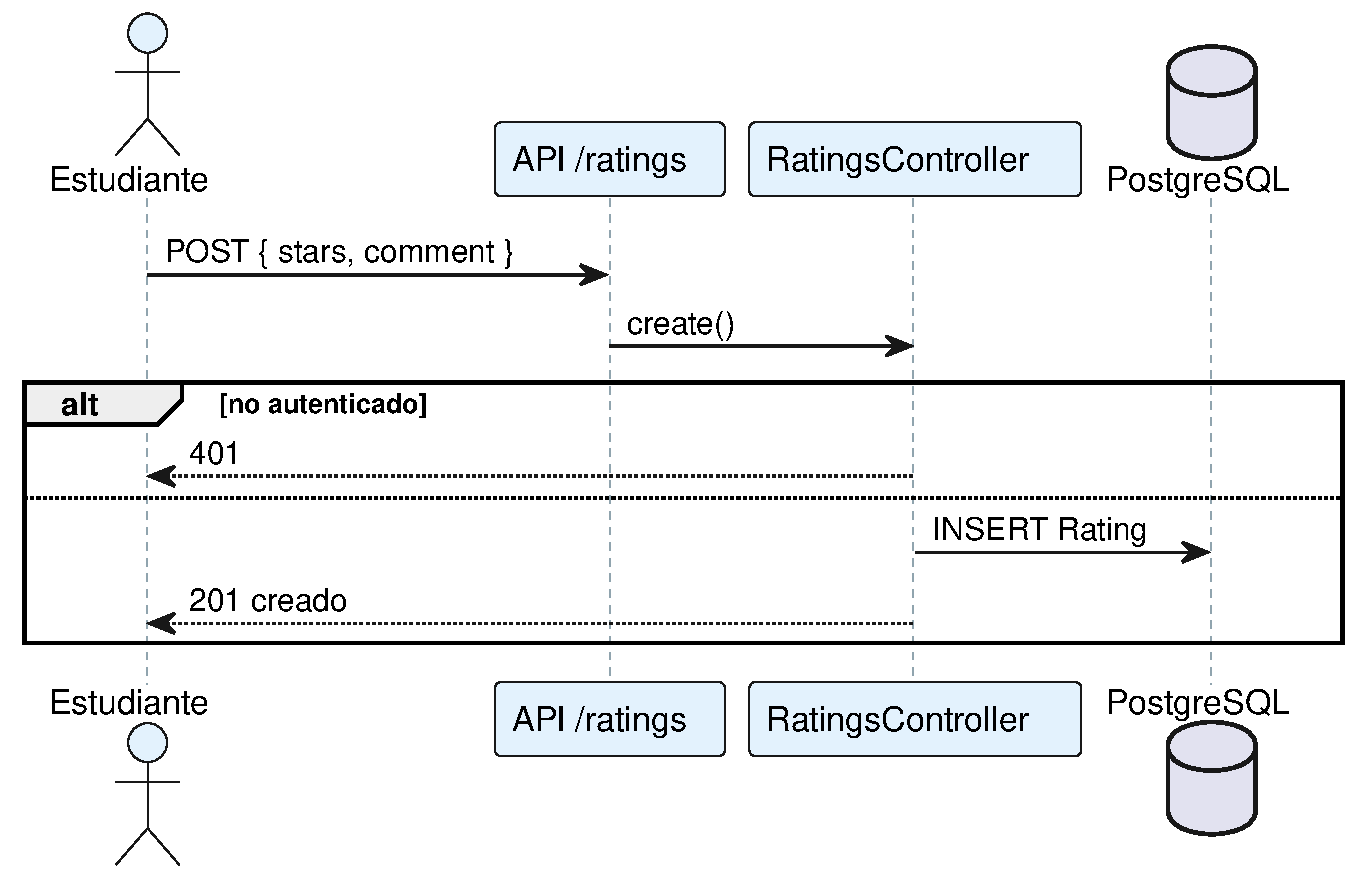
\includegraphics[width=\linewidth,height=0.42\textheight,keepaspectratio]{cu/cu18-seq.pdf}\caption{Diagrama de secuencia --- CU-18}\end{figure}
\begin{figure}[H]\centering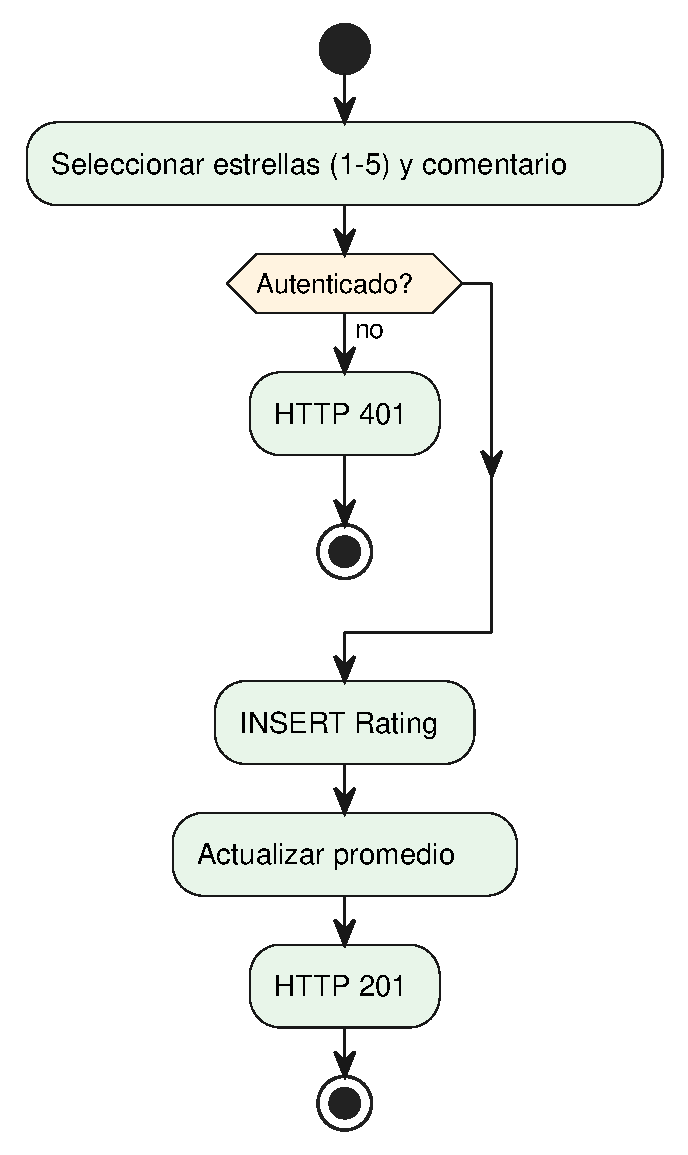
\includegraphics[width=\linewidth,height=0.46\textheight,keepaspectratio]{cu/cu18-act.pdf}\caption{Diagrama de actividades --- CU-18}\end{figure}

\subsection{CU-19 --- Enviar y responder quejas}

\noindent\textbf{Endpoint(s):} \texttt{POST /api/complaints, POST /api/complaints/:id/respond}\par\vspace{4pt}

\begin{table}[H]\centering\small
\caption{Ficha del caso de uso CU-19 --- Enviar y responder quejas}
\begin{tabularx}{\textwidth}{L{0.26\textwidth} X}
\toprule
\textbf{Campo} & \textbf{Descripcion} \\ \midrule
Objetivo del contexto & Permitir al estudiante enviar quejas, sugerencias o comentarios (anonimos o no) y al administrador responderlas. \\ \midrule
Precondiciones & El estudiante debe estar autenticado para enviar; el administrador para responder. \\ \midrule
Condicion de exito & Se registra la queja y, en su caso, la respuesta del administrador. \\ \midrule
Condicion de fracaso & Datos invalidos. \\ \midrule
Actores principales & Estudiante, Administrador \\ \midrule
Actores secundarios & Base de datos \\
\bottomrule\end{tabularx}\end{table}
\begin{table}[H]\centering\small
\caption{Flujo principal de CU-19}
\begin{tabularx}{\textwidth}{C{0.10\textwidth} X}
\toprule \textbf{Paso} & \textbf{Accion} \\ \midrule
1 & El estudiante crea una queja/sugerencia/comentario. \\
2 & Si es anonima, no se asocia al estudiante. \\
3 & El sistema registra la queja. \\
4 & El administrador responde y la marca como resuelta. \\
\bottomrule\end{tabularx}\end{table}
\begin{table}[H]\centering\small
\caption{Extensiones (flujos alternativos) de CU-19}
\begin{tabularx}{\textwidth}{C{0.10\textwidth} X}
\toprule \textbf{Paso} & \textbf{Accion} \\ \midrule
1.1 & Contenido vacio $\rightarrow$ HTTP 400. \\
\bottomrule\end{tabularx}\end{table}
\begin{figure}[H]\centering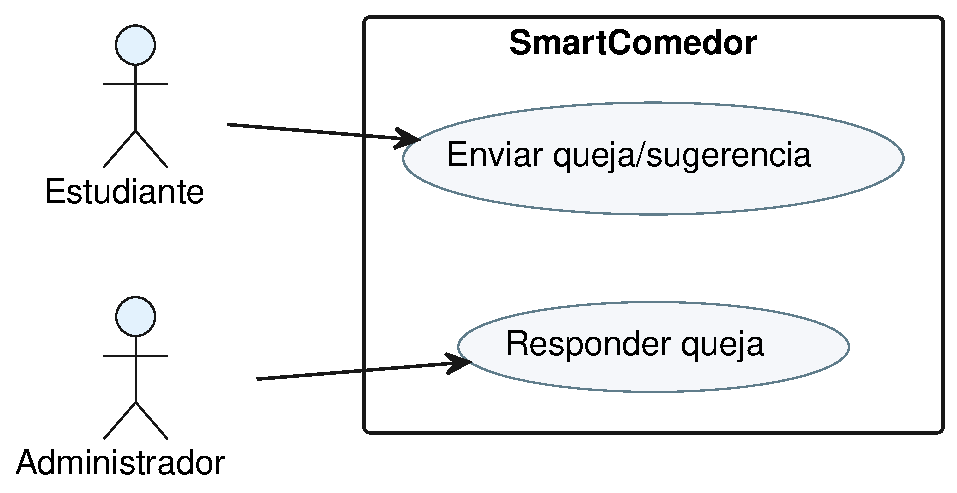
\includegraphics[width=\linewidth,height=0.30\textheight,keepaspectratio]{cu/cu19-uc.pdf}\caption{Diagrama de caso de uso --- CU-19}\end{figure}
\begin{figure}[H]\centering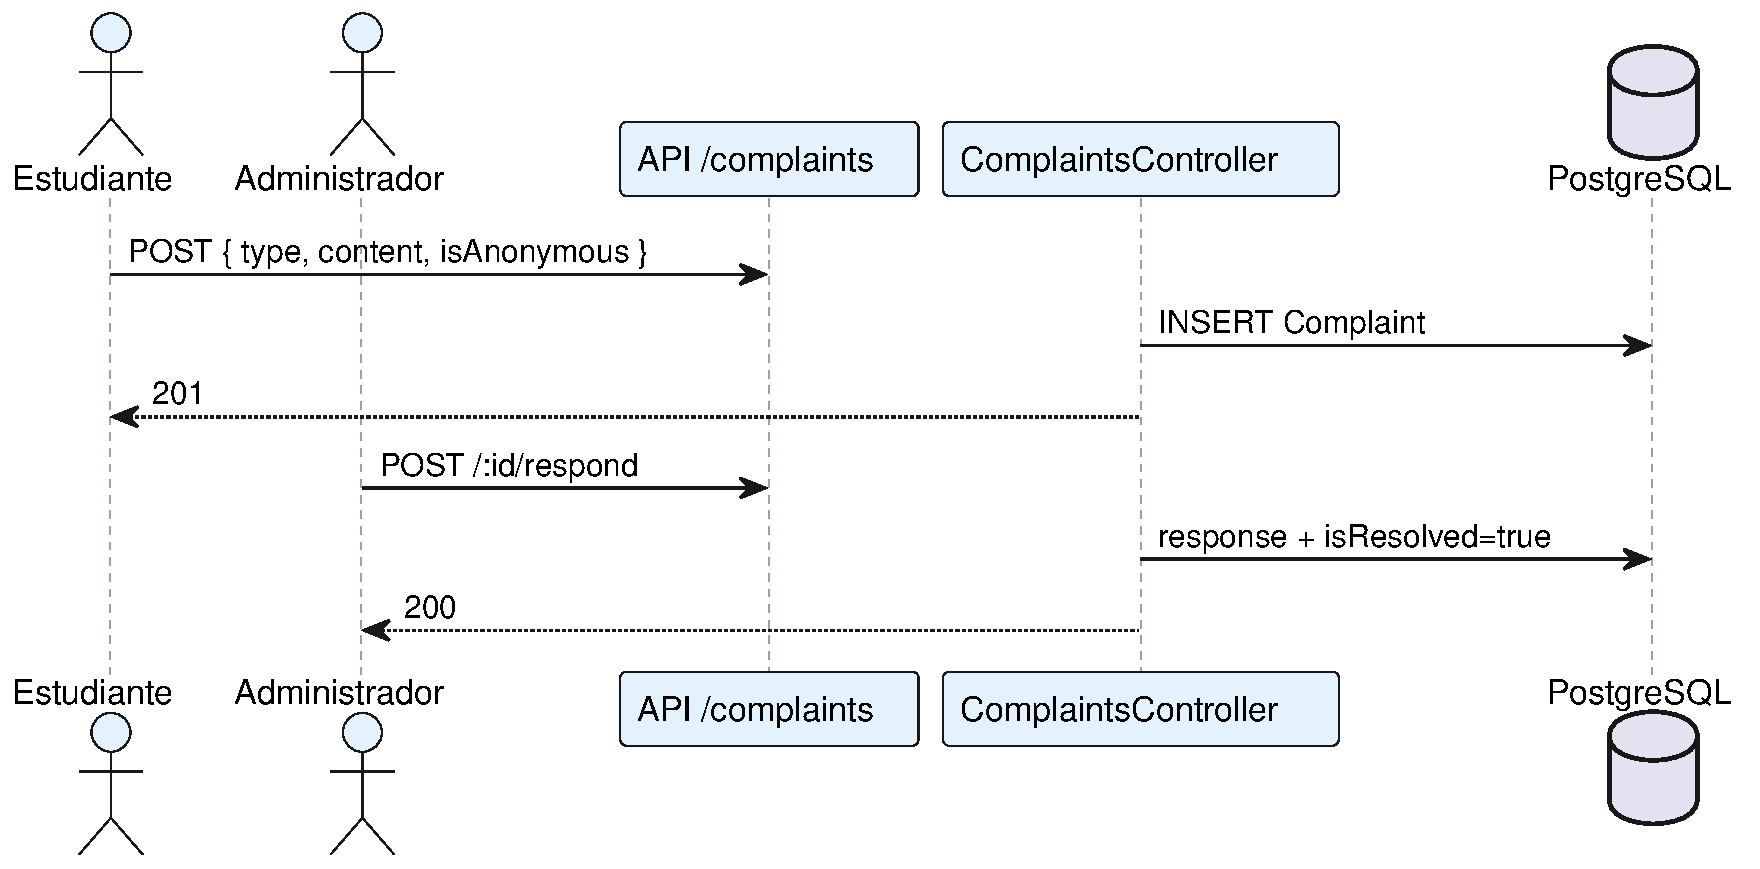
\includegraphics[width=\linewidth,height=0.42\textheight,keepaspectratio]{cu/cu19-seq.pdf}\caption{Diagrama de secuencia --- CU-19}\end{figure}
\begin{figure}[H]\centering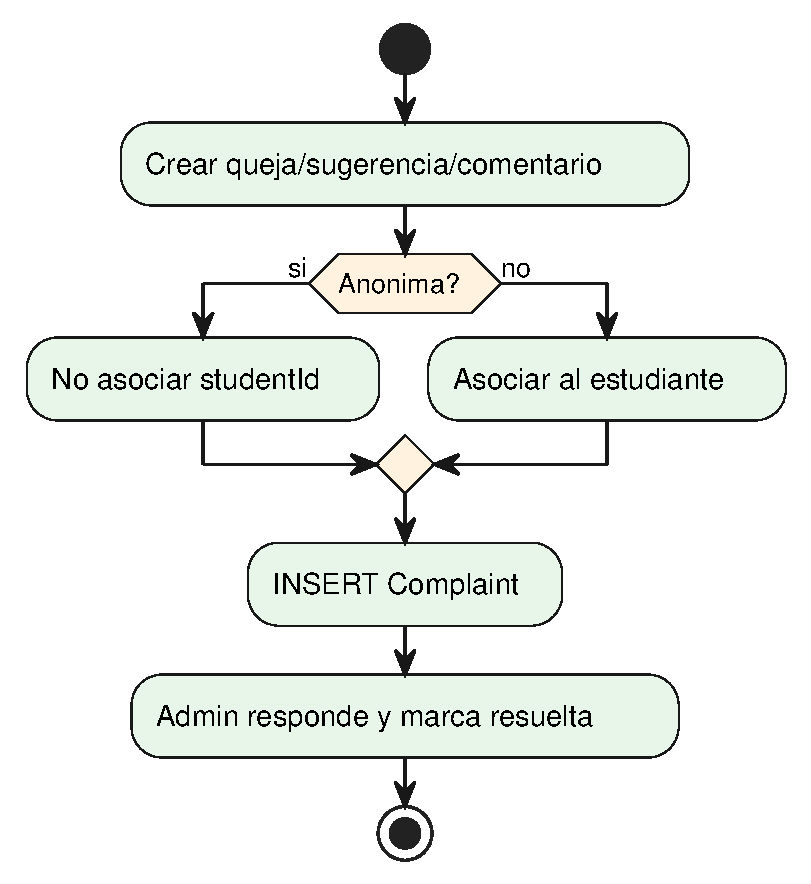
\includegraphics[width=\linewidth,height=0.46\textheight,keepaspectratio]{cu/cu19-act.pdf}\caption{Diagrama de actividades --- CU-19}\end{figure}

\subsection{CU-20 --- Gestionar noticias}

\noindent\textbf{Endpoint(s):} \texttt{GET/POST/PUT/DELETE /api/news}\par\vspace{4pt}

\begin{table}[H]\centering\small
\caption{Ficha del caso de uso CU-20 --- Gestionar noticias}
\begin{tabularx}{\textwidth}{L{0.26\textwidth} X}
\toprule
\textbf{Campo} & \textbf{Descripcion} \\ \midrule
Objetivo del contexto & Permitir al administrador publicar, editar y eliminar noticias visibles para los usuarios. \\ \midrule
Precondiciones & El administrador debe estar autenticado con rol admin. \\ \midrule
Condicion de exito & La noticia se crea, actualiza o desactiva. \\ \midrule
Condicion de fracaso & Datos invalidos o noticia inexistente. \\ \midrule
Actores principales & Administrador, Usuario \\ \midrule
Actores secundarios & Base de datos \\
\bottomrule\end{tabularx}\end{table}
\begin{table}[H]\centering\small
\caption{Flujo principal de CU-20}
\begin{tabularx}{\textwidth}{C{0.10\textwidth} X}
\toprule \textbf{Paso} & \textbf{Accion} \\ \midrule
1 & El administrador selecciona la operacion sobre la noticia. \\
2 & El sistema valida los datos. \\
3 & El sistema crea, actualiza o desactiva (soft delete) la noticia. \\
4 & Los usuarios consultan las noticias activas. \\
\bottomrule\end{tabularx}\end{table}
\begin{table}[H]\centering\small
\caption{Extensiones (flujos alternativos) de CU-20}
\begin{tabularx}{\textwidth}{C{0.10\textwidth} X}
\toprule \textbf{Paso} & \textbf{Accion} \\ \midrule
2.1 & Datos invalidos $\rightarrow$ HTTP 400. \\
3.1 & Noticia inexistente $\rightarrow$ HTTP 404. \\
\bottomrule\end{tabularx}\end{table}
\begin{figure}[H]\centering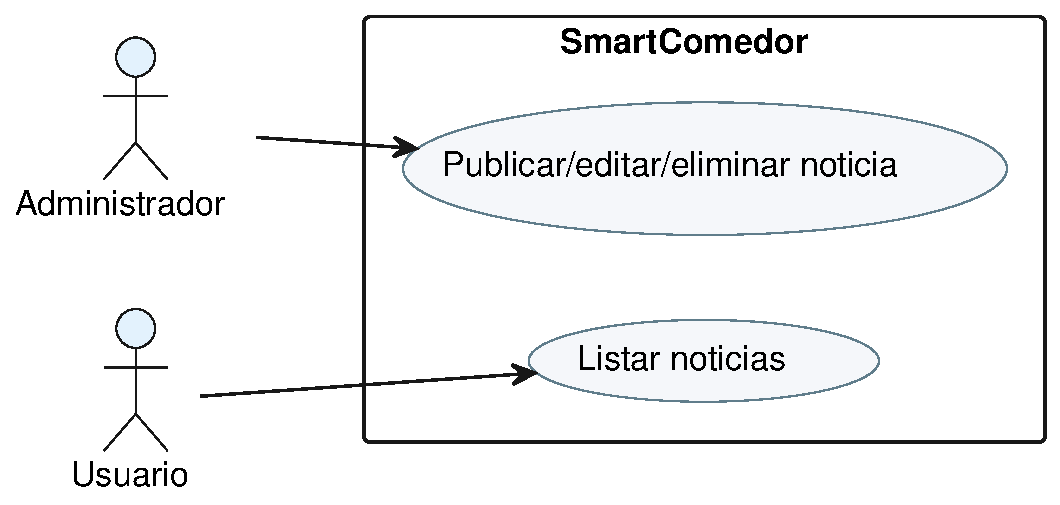
\includegraphics[width=\linewidth,height=0.30\textheight,keepaspectratio]{cu/cu20-uc.pdf}\caption{Diagrama de caso de uso --- CU-20}\end{figure}
\begin{figure}[H]\centering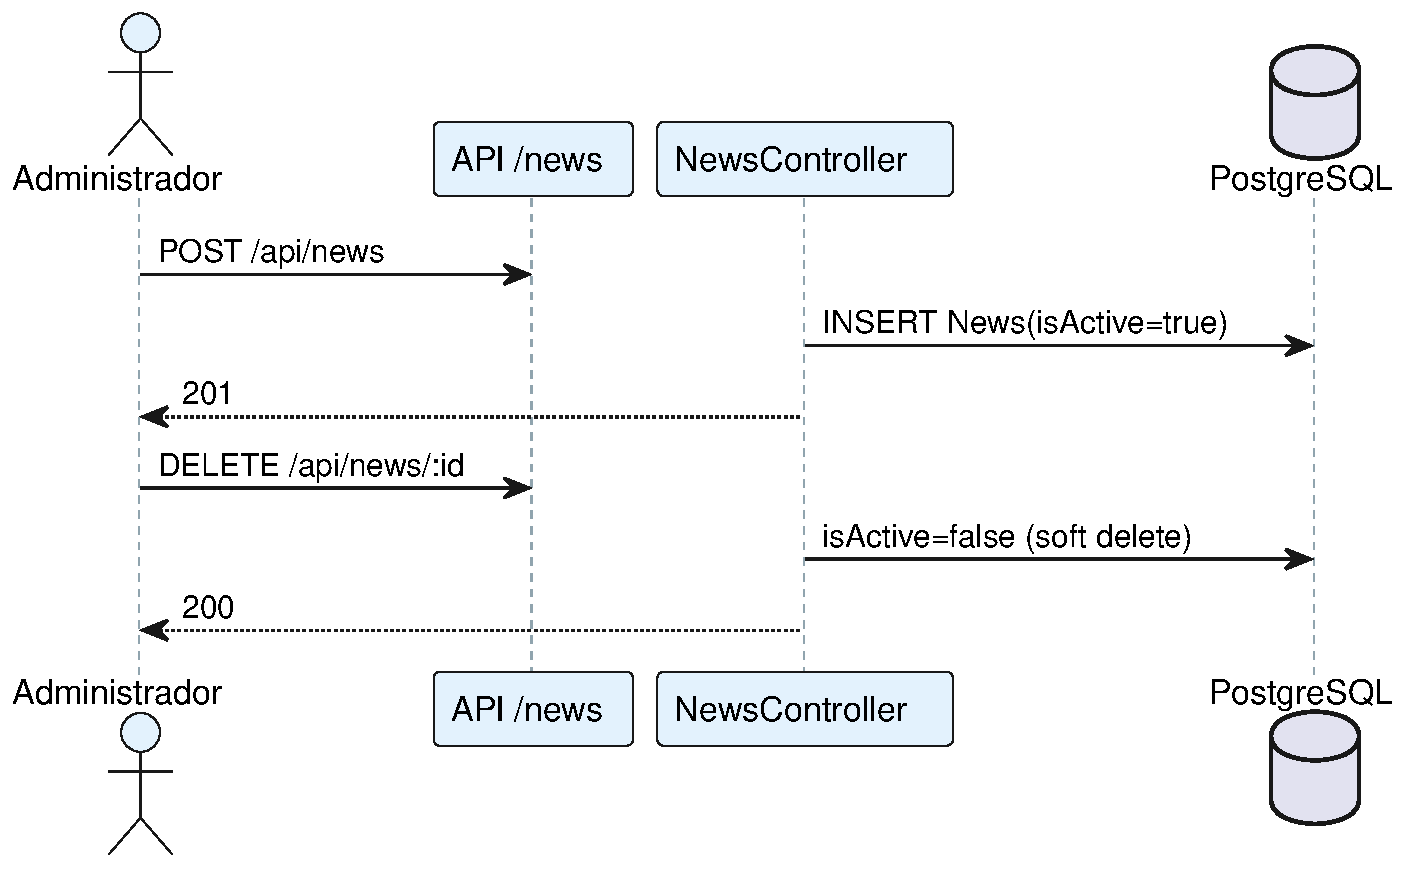
\includegraphics[width=\linewidth,height=0.42\textheight,keepaspectratio]{cu/cu20-seq.pdf}\caption{Diagrama de secuencia --- CU-20}\end{figure}
\begin{figure}[H]\centering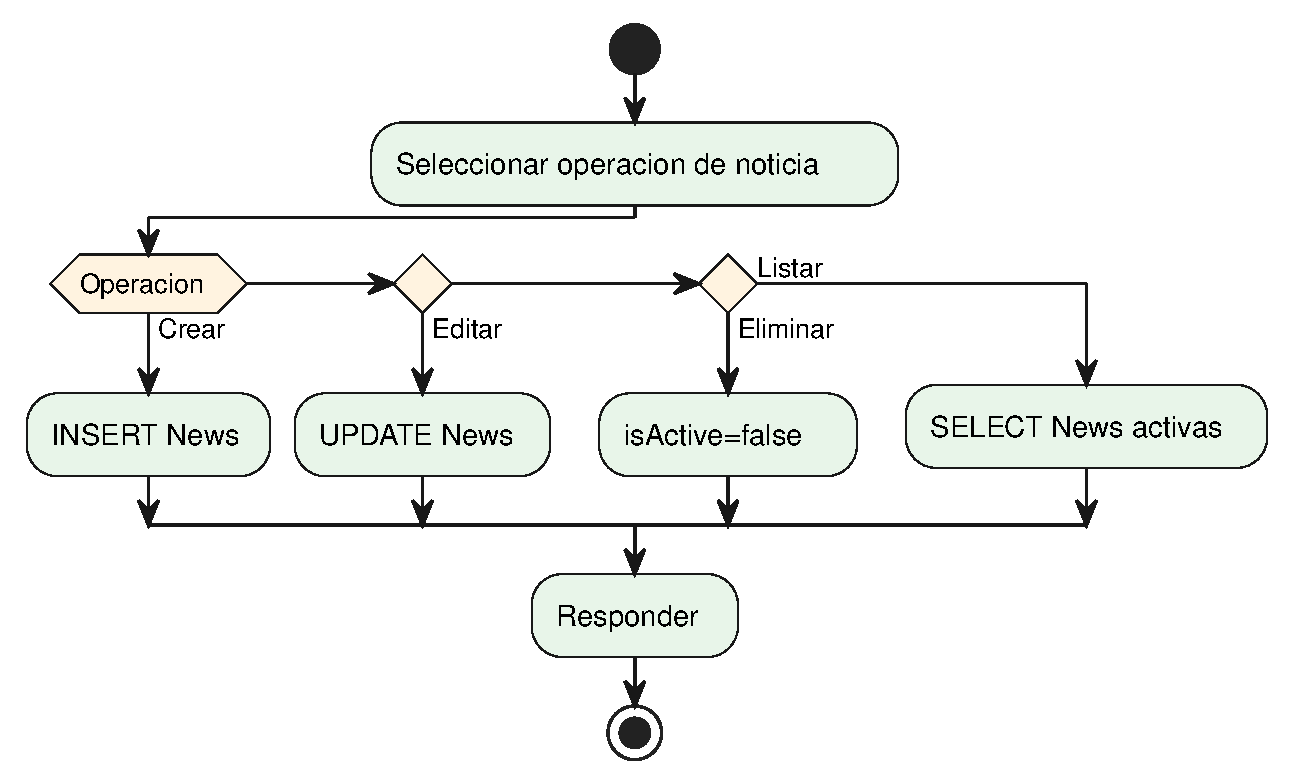
\includegraphics[width=\linewidth,height=0.46\textheight,keepaspectratio]{cu/cu20-act.pdf}\caption{Diagrama de actividades --- CU-20}\end{figure}

\subsection{CU-21 --- Consultar auditoria}

\noindent\textbf{Endpoint(s):} \texttt{GET /api/audit}\par\vspace{4pt}

\begin{table}[H]\centering\small
\caption{Ficha del caso de uso CU-21 --- Consultar auditoria}
\begin{tabularx}{\textwidth}{L{0.26\textwidth} X}
\toprule
\textbf{Campo} & \textbf{Descripcion} \\ \midrule
Objetivo del contexto & Permitir a los perfiles autorizados consultar la bitacora de auditoria del sistema con filtros controlados. \\ \midrule
Precondiciones & El usuario debe tener rol admin o auditor. \\ \midrule
Condicion de exito & Se devuelven los eventos de auditoria paginados. \\ \midrule
Condicion de fracaso & Filtros fuera de la lista blanca. \\ \midrule
Actores principales & Administrador, Auditor externo \\ \midrule
Actores secundarios & Base de datos \\
\bottomrule\end{tabularx}\end{table}
\begin{table}[H]\centering\small
\caption{Flujo principal de CU-21}
\begin{tabularx}{\textwidth}{C{0.10\textwidth} X}
\toprule \textbf{Paso} & \textbf{Accion} \\ \midrule
1 & El usuario ingresa filtros (accion, metodo, fechas). \\
2 & El sistema valida los filtros contra una lista blanca. \\
3 & El sistema consulta audit\_logs con paginacion. \\
4 & El sistema responde 200 con los eventos. \\
\bottomrule\end{tabularx}\end{table}
\begin{table}[H]\centering\small
\caption{Extensiones (flujos alternativos) de CU-21}
\begin{tabularx}{\textwidth}{C{0.10\textwidth} X}
\toprule \textbf{Paso} & \textbf{Accion} \\ \midrule
2.1 & Filtro no permitido $\rightarrow$ HTTP 400. \\
\bottomrule\end{tabularx}\end{table}
\begin{figure}[H]\centering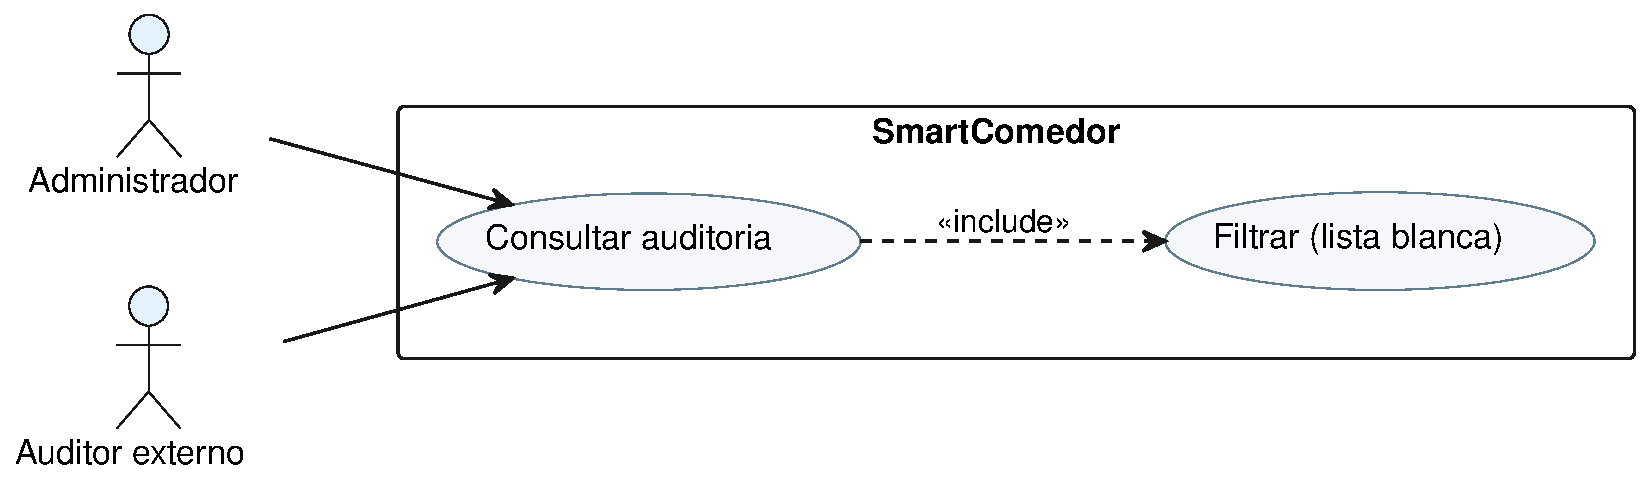
\includegraphics[width=\linewidth,height=0.30\textheight,keepaspectratio]{cu/cu21-uc.pdf}\caption{Diagrama de caso de uso --- CU-21}\end{figure}
\begin{figure}[H]\centering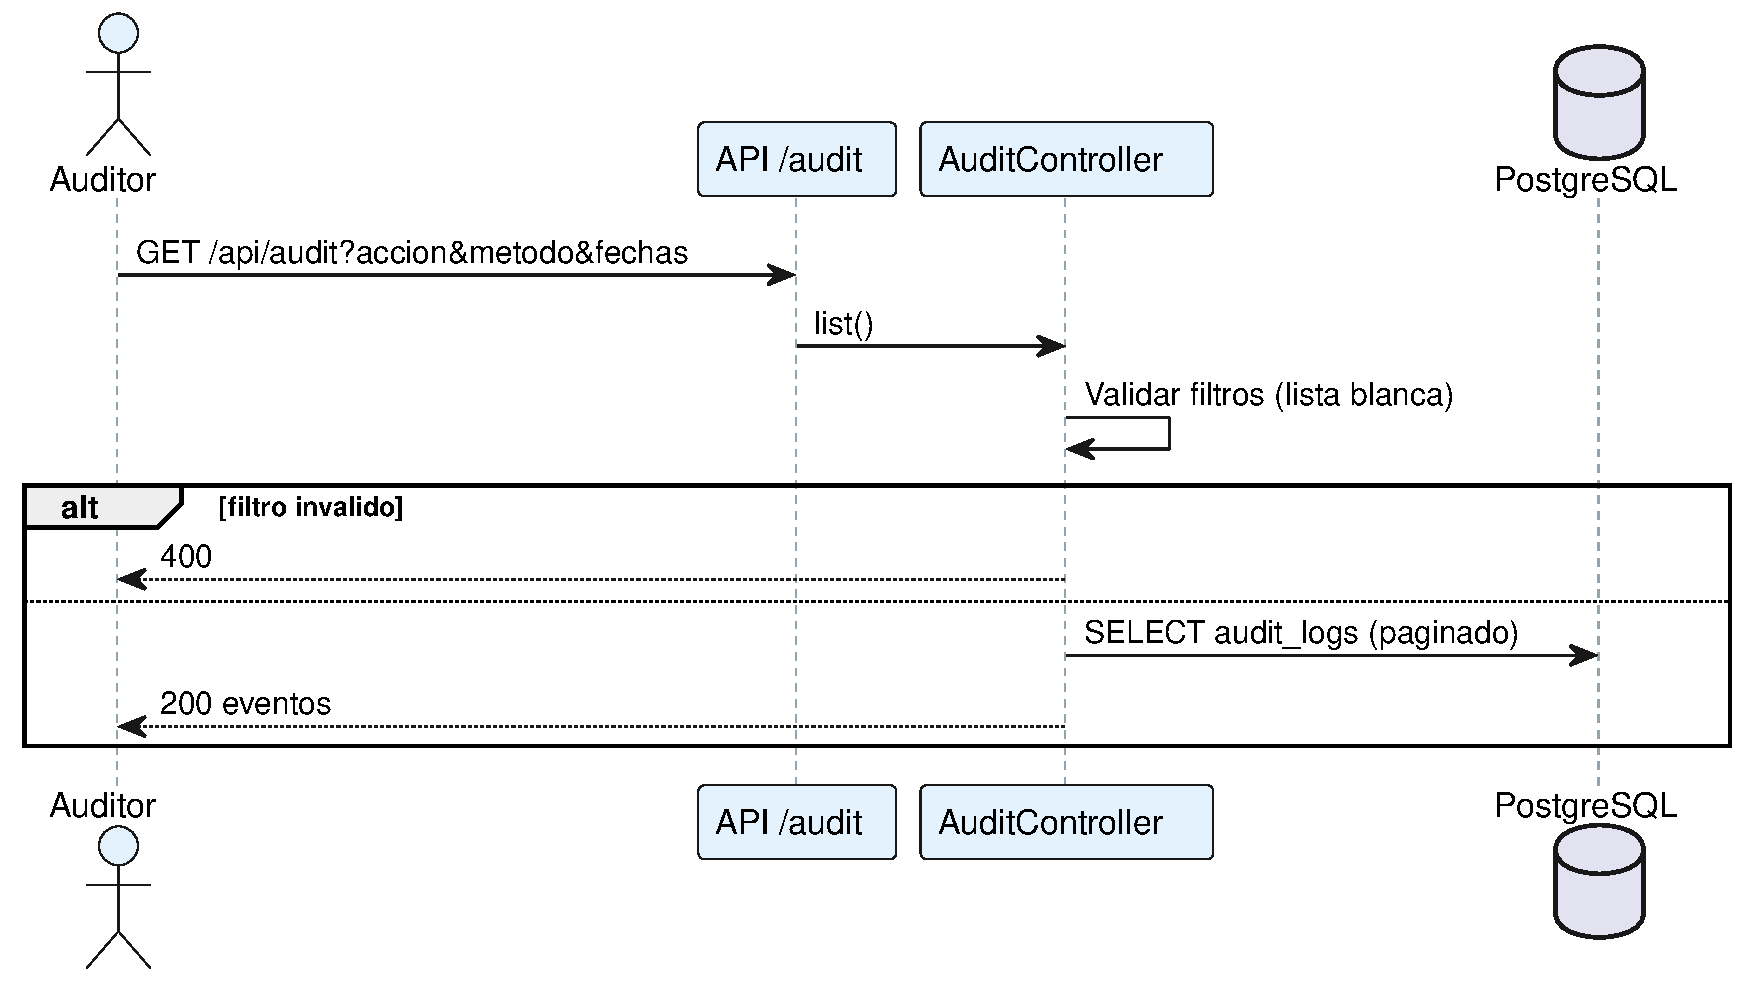
\includegraphics[width=\linewidth,height=0.42\textheight,keepaspectratio]{cu/cu21-seq.pdf}\caption{Diagrama de secuencia --- CU-21}\end{figure}
\begin{figure}[H]\centering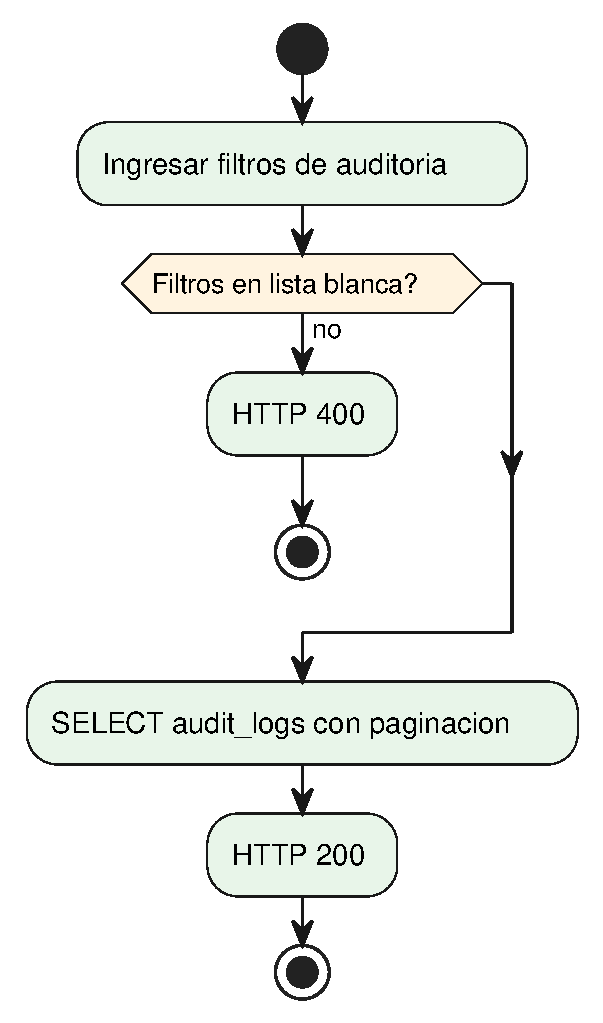
\includegraphics[width=\linewidth,height=0.46\textheight,keepaspectratio]{cu/cu21-act.pdf}\caption{Diagrama de actividades --- CU-21}\end{figure}



\section{Modelo de diseño del sistema}

\subsection{Diagrama de clases detallado}
El modelo de dominio se implementa con Sequelize. La Figura~\ref{fig:clases} muestra el
diagrama de clases. Todas las entidades incluyen \texttt{id} (UUID, PK), \texttt{uid}
(identificador legible único con prefijo por tipo, generado en el hook
\texttt{beforeValidate}), \texttt{createdAt} y \texttt{updatedAt}.

\begin{figure}[H]
\centering
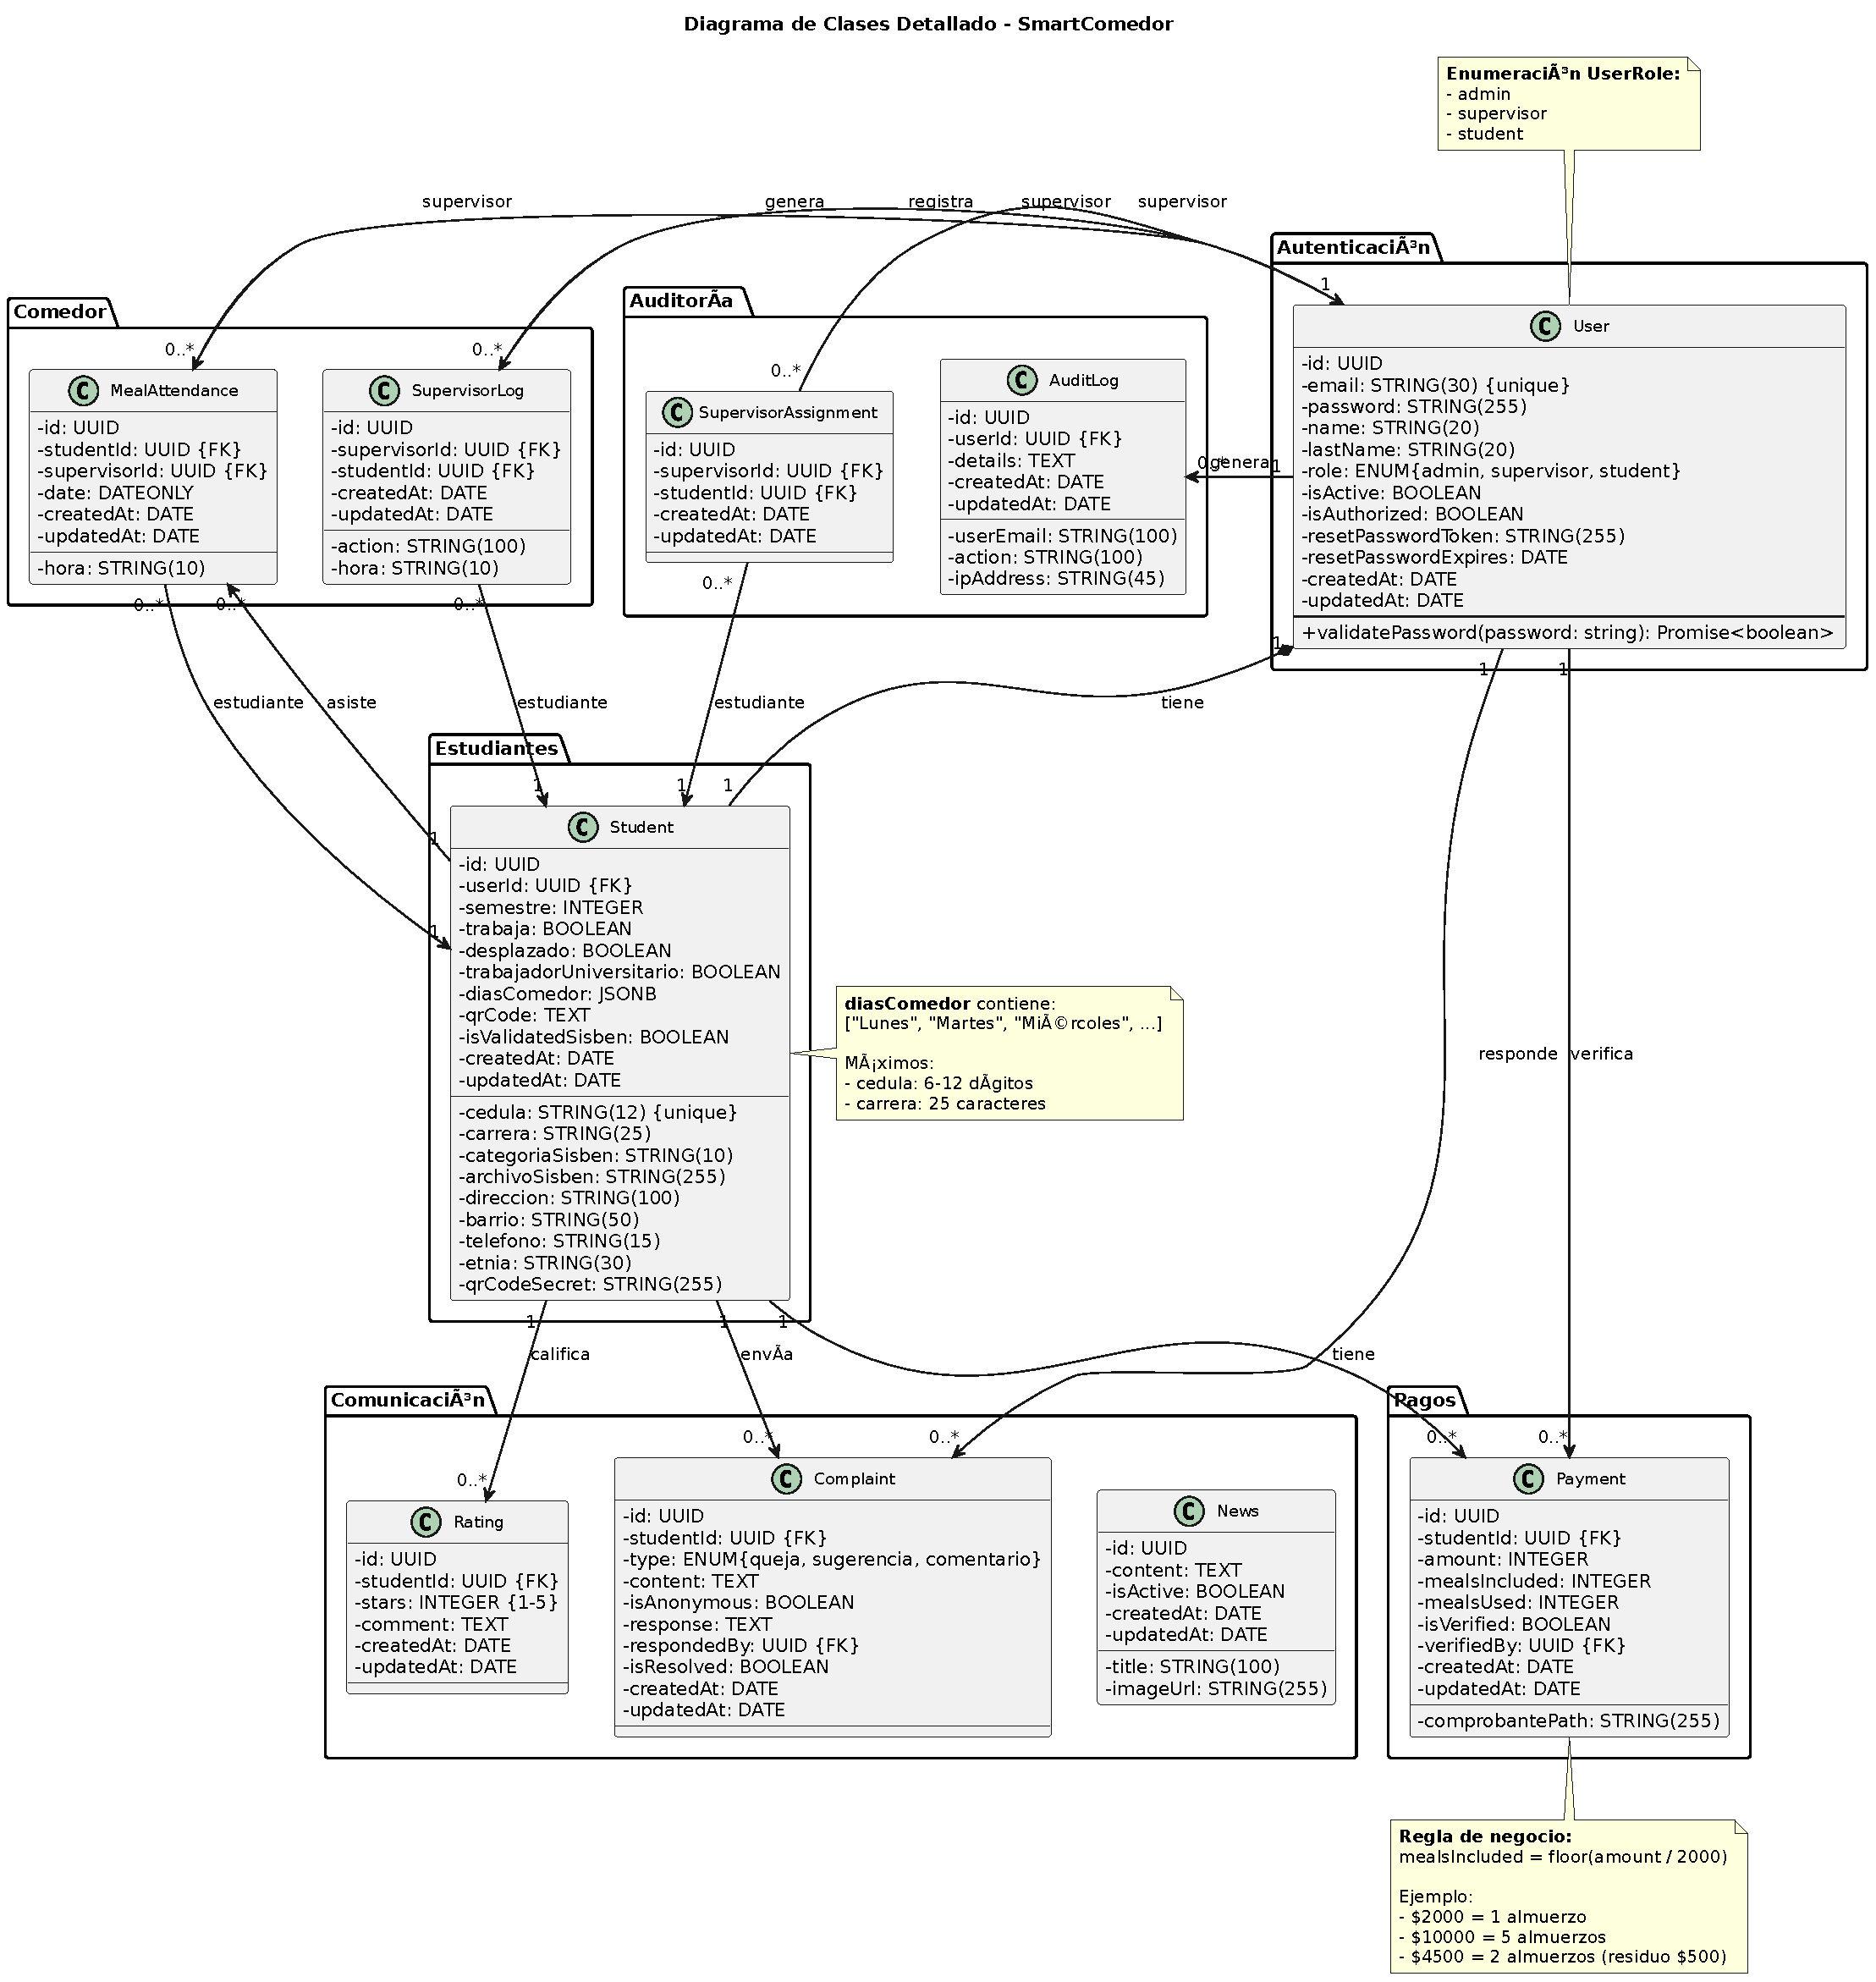
\includegraphics[width=\textwidth]{figs/class-diagram.pdf}
\caption{Diagrama de clases del dominio.}
\label{fig:clases}
\end{figure}

La Tabla~\ref{tab:entidades} resume las entidades principales y sus atributos
representativos.

\begin{longtable}{L{0.20\textwidth} L{0.74\textwidth}}
\caption{Entidades principales y atributos representativos}\label{tab:entidades}\\
\toprule
\textbf{Entidad (tabla)} & \textbf{Atributos representativos} \\
\midrule
\endfirsthead
\toprule
\textbf{Entidad (tabla)} & \textbf{Atributos representativos} \\
\midrule
\endhead
\bottomrule
\endlastfoot
User (\texttt{users}) & email (único), password (hash), name, lastName, telefono, role, isActive, isAuthorized, diasAsignados, resetPasswordToken/Expires; método \texttt{validatePassword}. \\
Student (\texttt{students}) & userId (FK), cedula, carrera, semestre, categoriaSisben, archivoSisben, cedulaFrontalPath, horarioPdfPath, direccion, barrio, telefono, trabaja, etnia, desplazado, diasComedor, qrCode/qrCodeSecret, isValidatedSisben, sisbenValidationDetails, currentCycle, cycleRevalidationDueAt. \\
Payment (\texttt{payments}) & studentId (FK), amount, mealsIncluded, mealsUsed, comprobantePath, universityReceiptPath, bankReceiptPath, isVerified, verifiedBy, verifiedAt. \\
MealAttendance (\texttt{meal\_attendances}) & studentId (FK), supervisorId (FK), date, hora. \\
SupervisorAssignment (\texttt{supervisor\_assignments}) & supervisorId (FK), studentId (FK) — relación N:M. \\
SupervisorLog (\texttt{supervisor\_logs}) & supervisorId (FK), studentId (FK), action, hora. \\
Rating (\texttt{ratings}) & studentId (FK), stars (1--5), comment. \\
Complaint (\texttt{complaints}) & studentId (FK, opcional), type (queja/sugerencia/comentario), content, isAnonymous, response, respondedBy, isResolved. \\
News (\texttt{news}) & title, content, imageUrl, isActive. \\
Cycle (\texttt{cycles}) & name, startDate, endDate, status (Activo/Cerrado). \\
AuditLog (\texttt{audit\_logs}) & userId, userEmail, action, details, ipAddress. \\
\end{longtable}

\subsection{Diagramas de secuencias}
Se documentan las secuencias de los flujos críticos: inicio de sesión
(Figura~\ref{fig:seq-login}), registro de estudiante (Figura~\ref{fig:seq-register}),
pago (Figura~\ref{fig:seq-payment}), registro de almuerzo (Figura~\ref{fig:seq-meal}) y
validación SISBÉN (Figura~\ref{fig:seq-sisben}).

\begin{figure}[H]
\centering
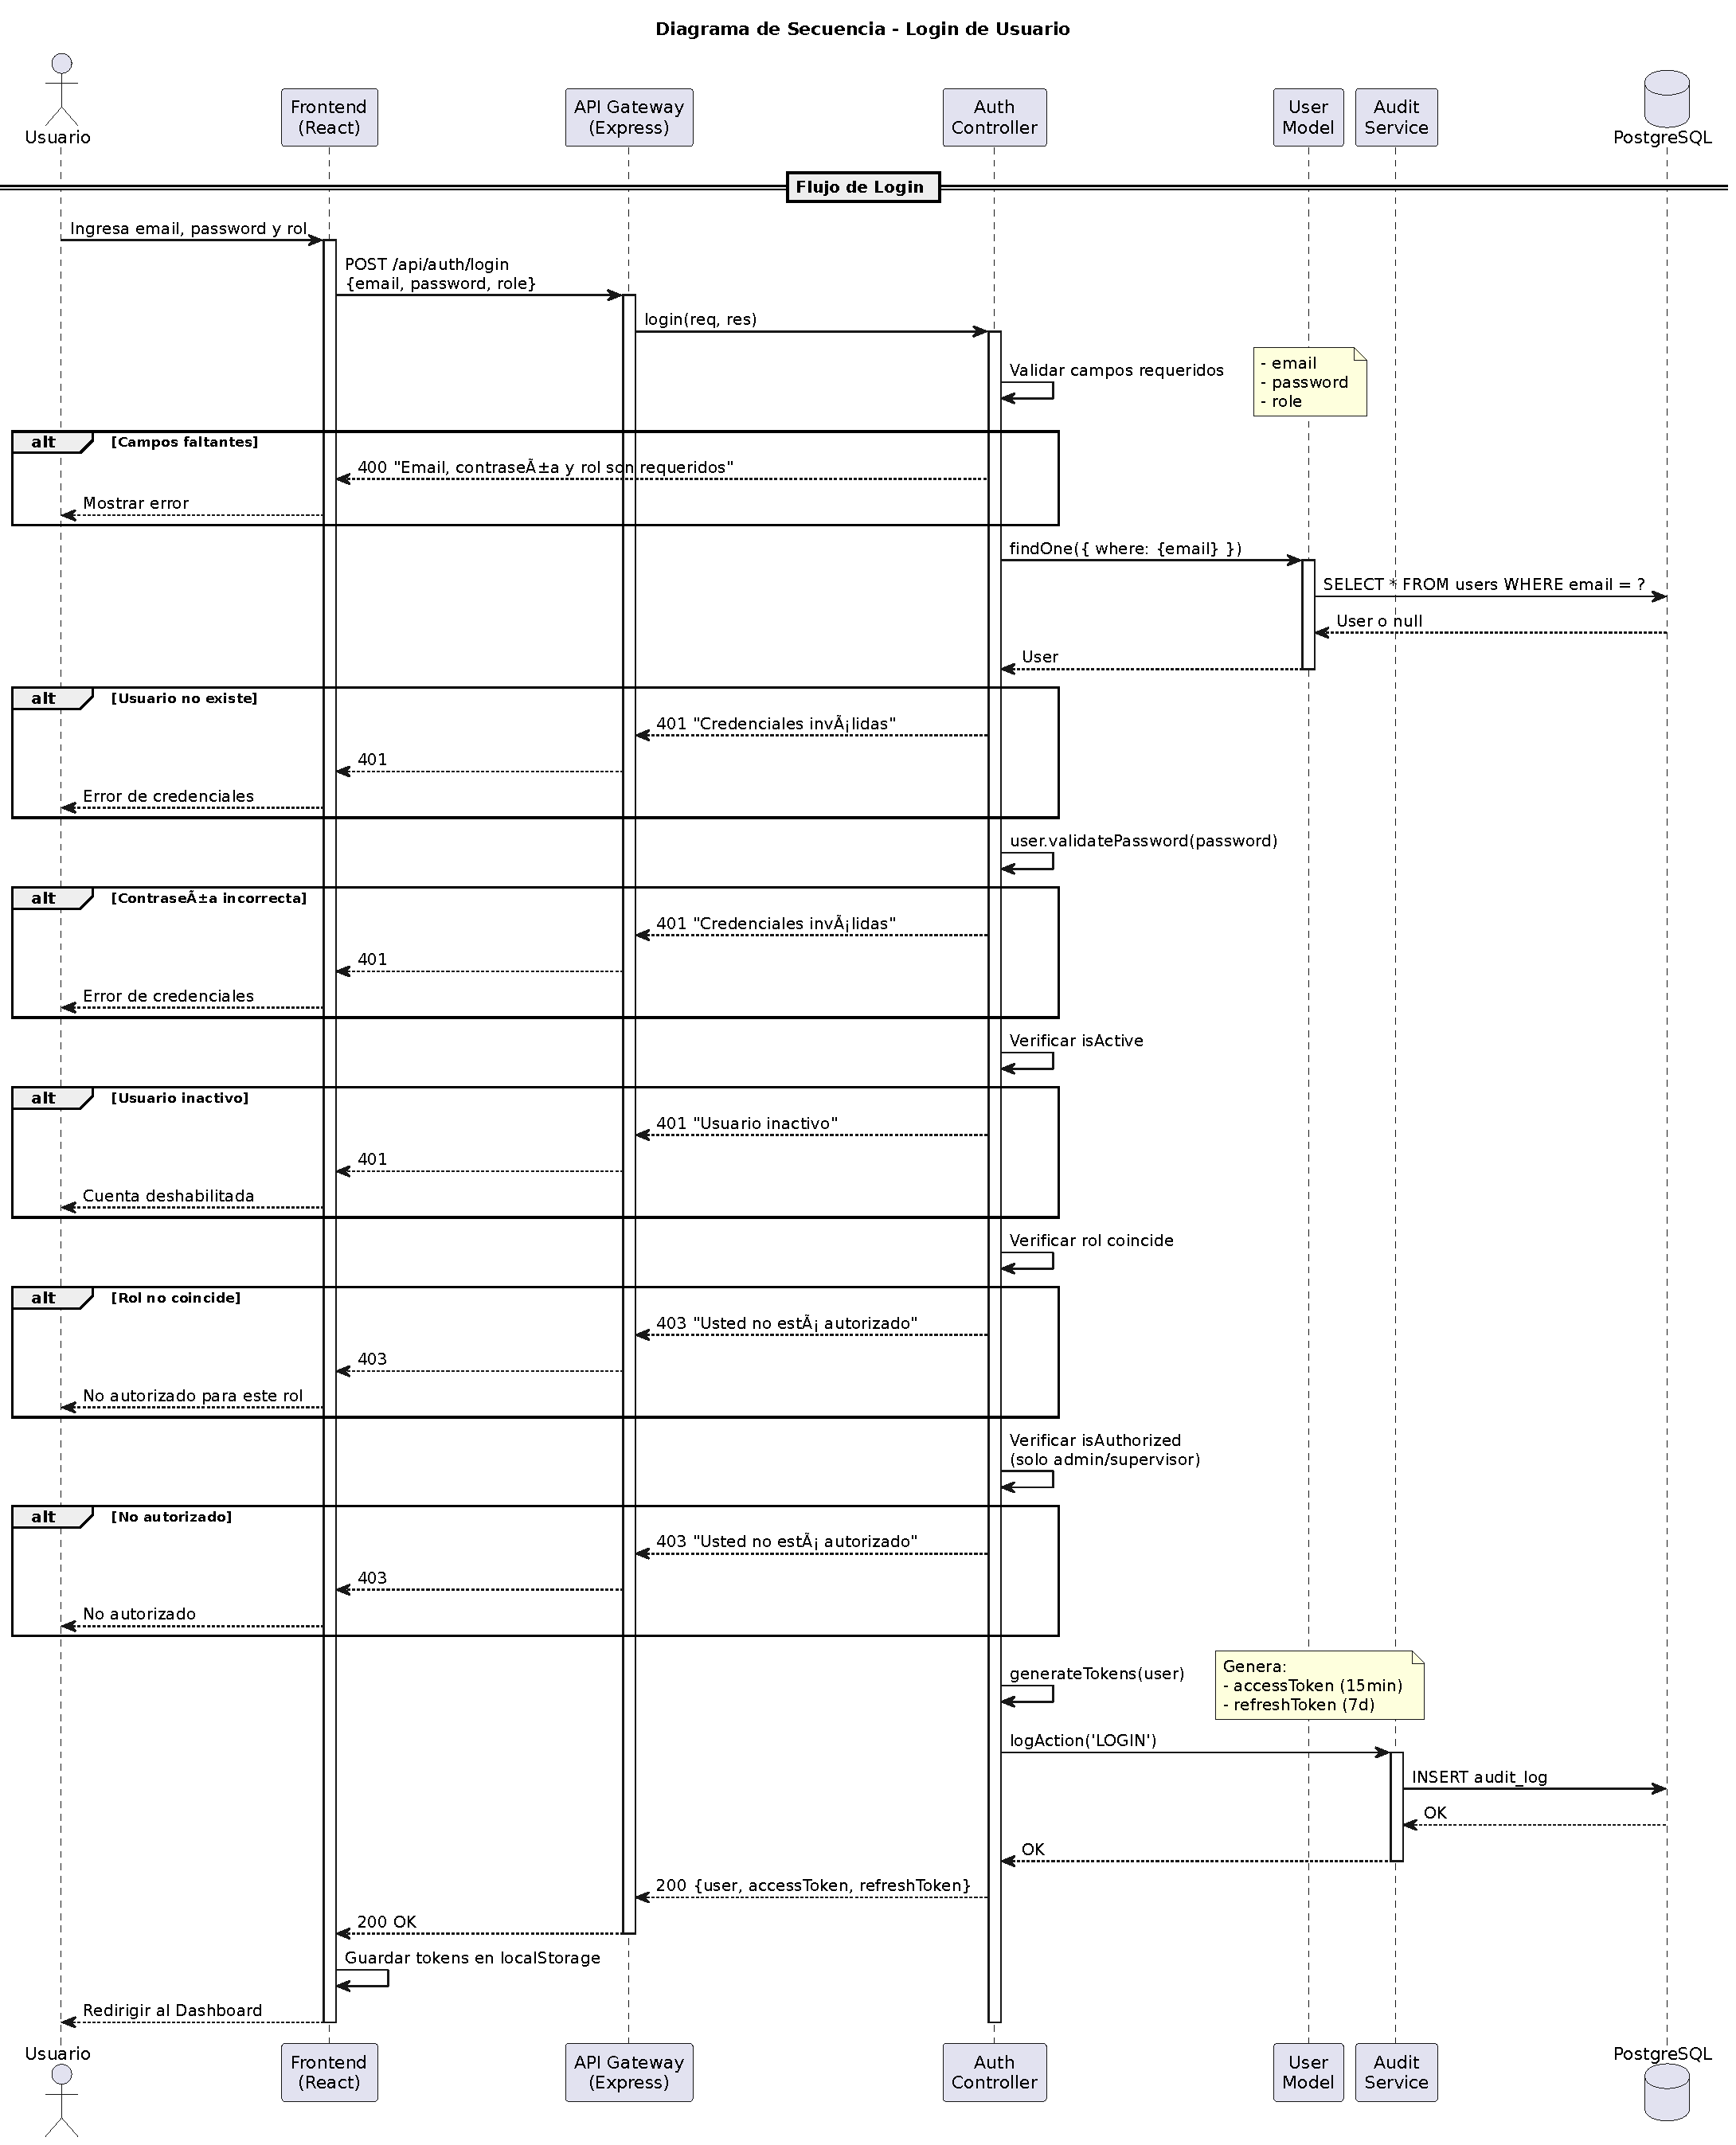
\includegraphics[width=0.92\textwidth]{figs/sequence-login.pdf}
\caption{Diagrama de secuencia — Inicio de sesión.}
\label{fig:seq-login}
\end{figure}

\begin{figure}[H]
\centering
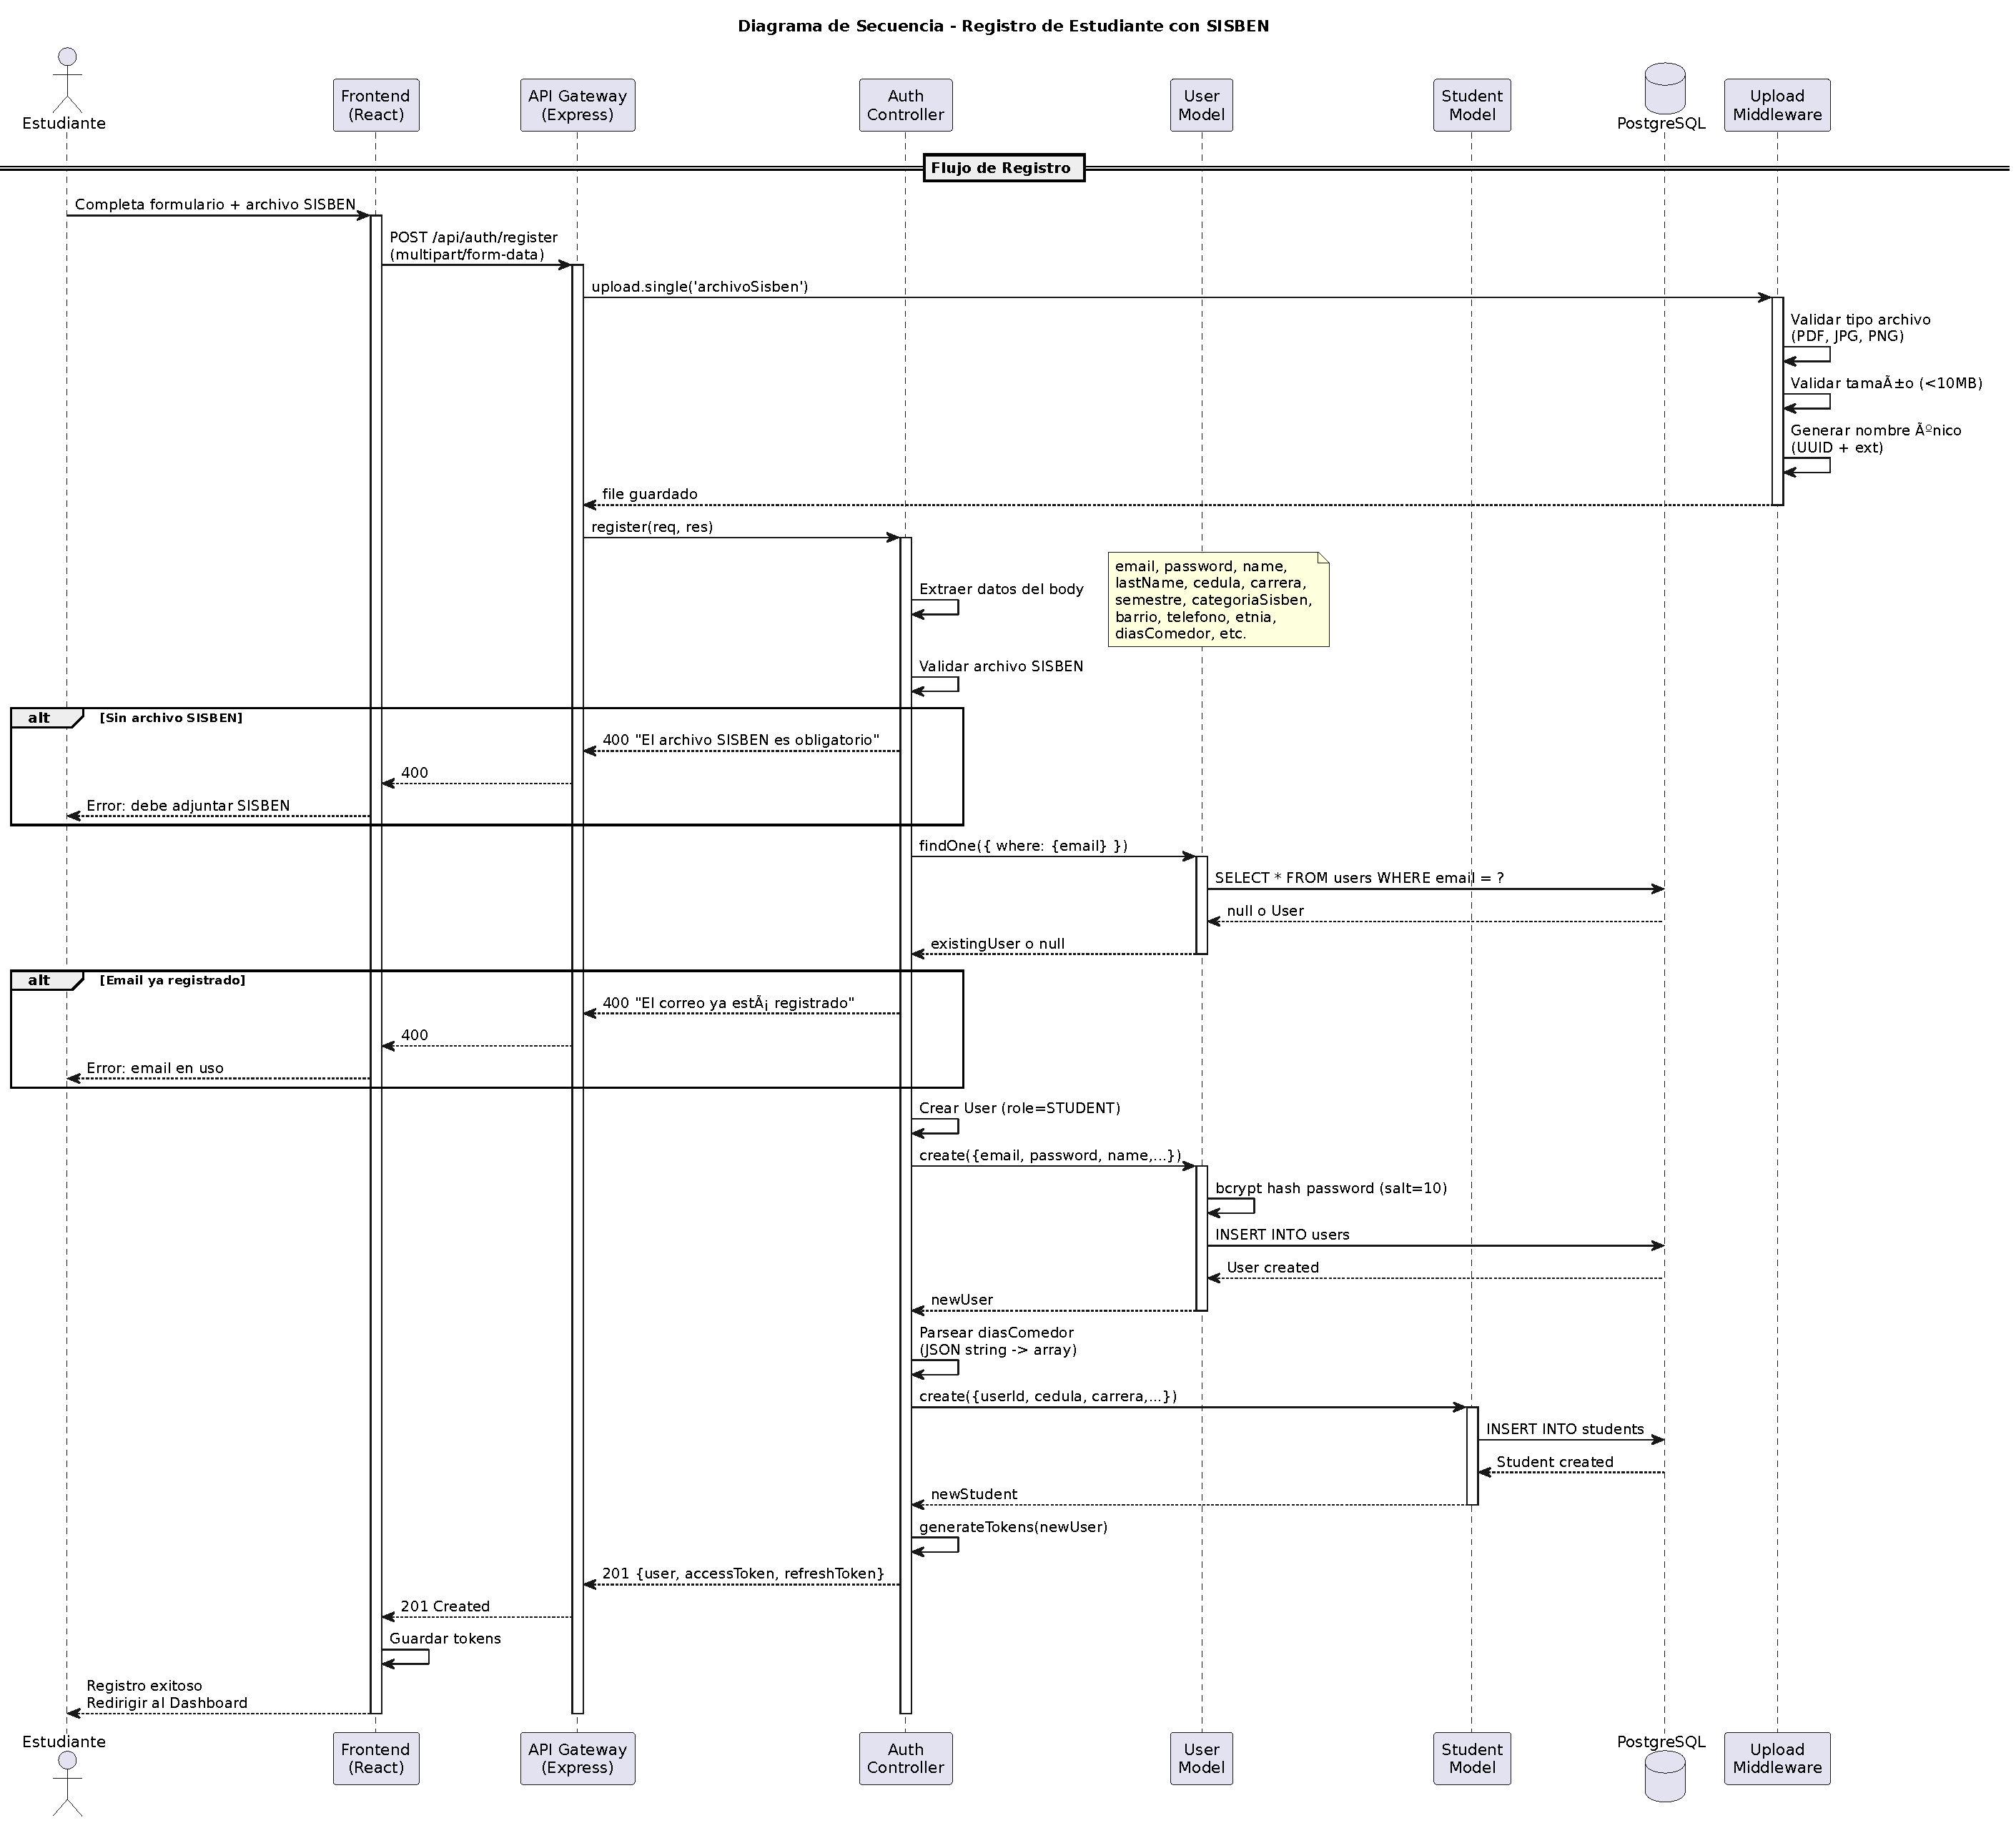
\includegraphics[width=0.92\textwidth]{figs/sequence-register.pdf}
\caption{Diagrama de secuencia — Registro de estudiante.}
\label{fig:seq-register}
\end{figure}

\begin{figure}[H]
\centering
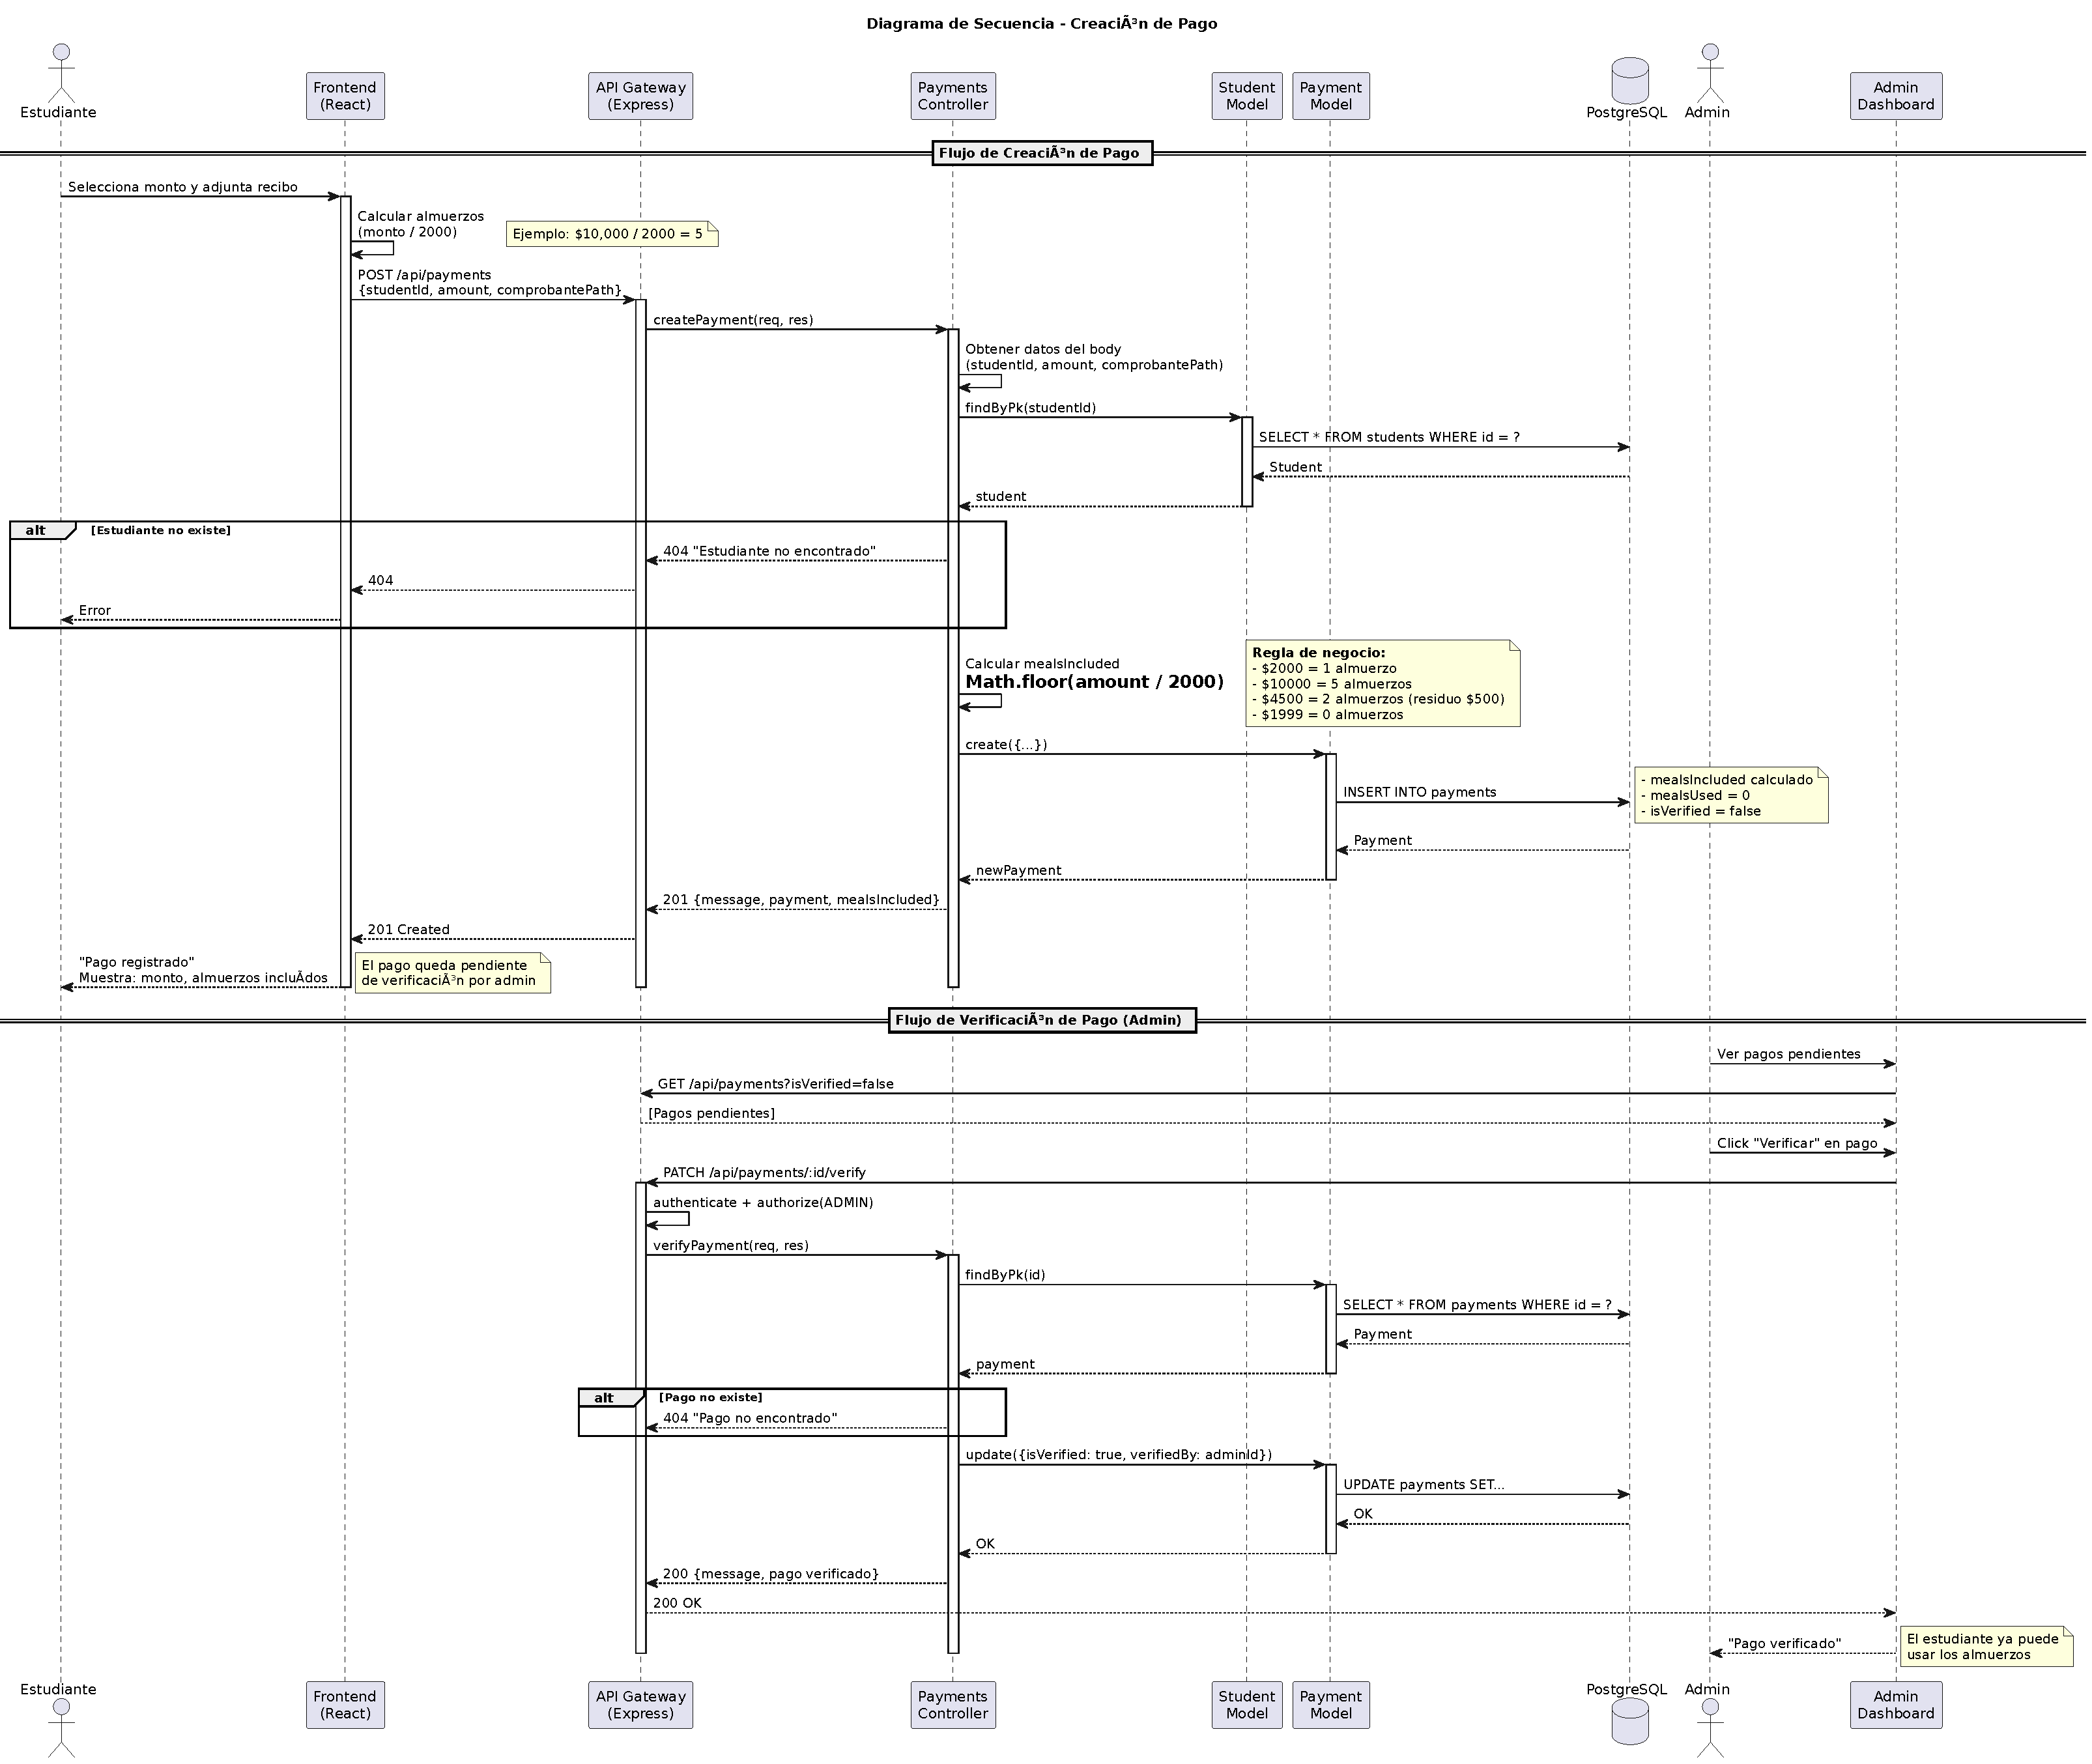
\includegraphics[width=0.92\textwidth]{figs/sequence-payment.pdf}
\caption{Diagrama de secuencia — Subida y verificación de pago.}
\label{fig:seq-payment}
\end{figure}

\begin{figure}[H]
\centering
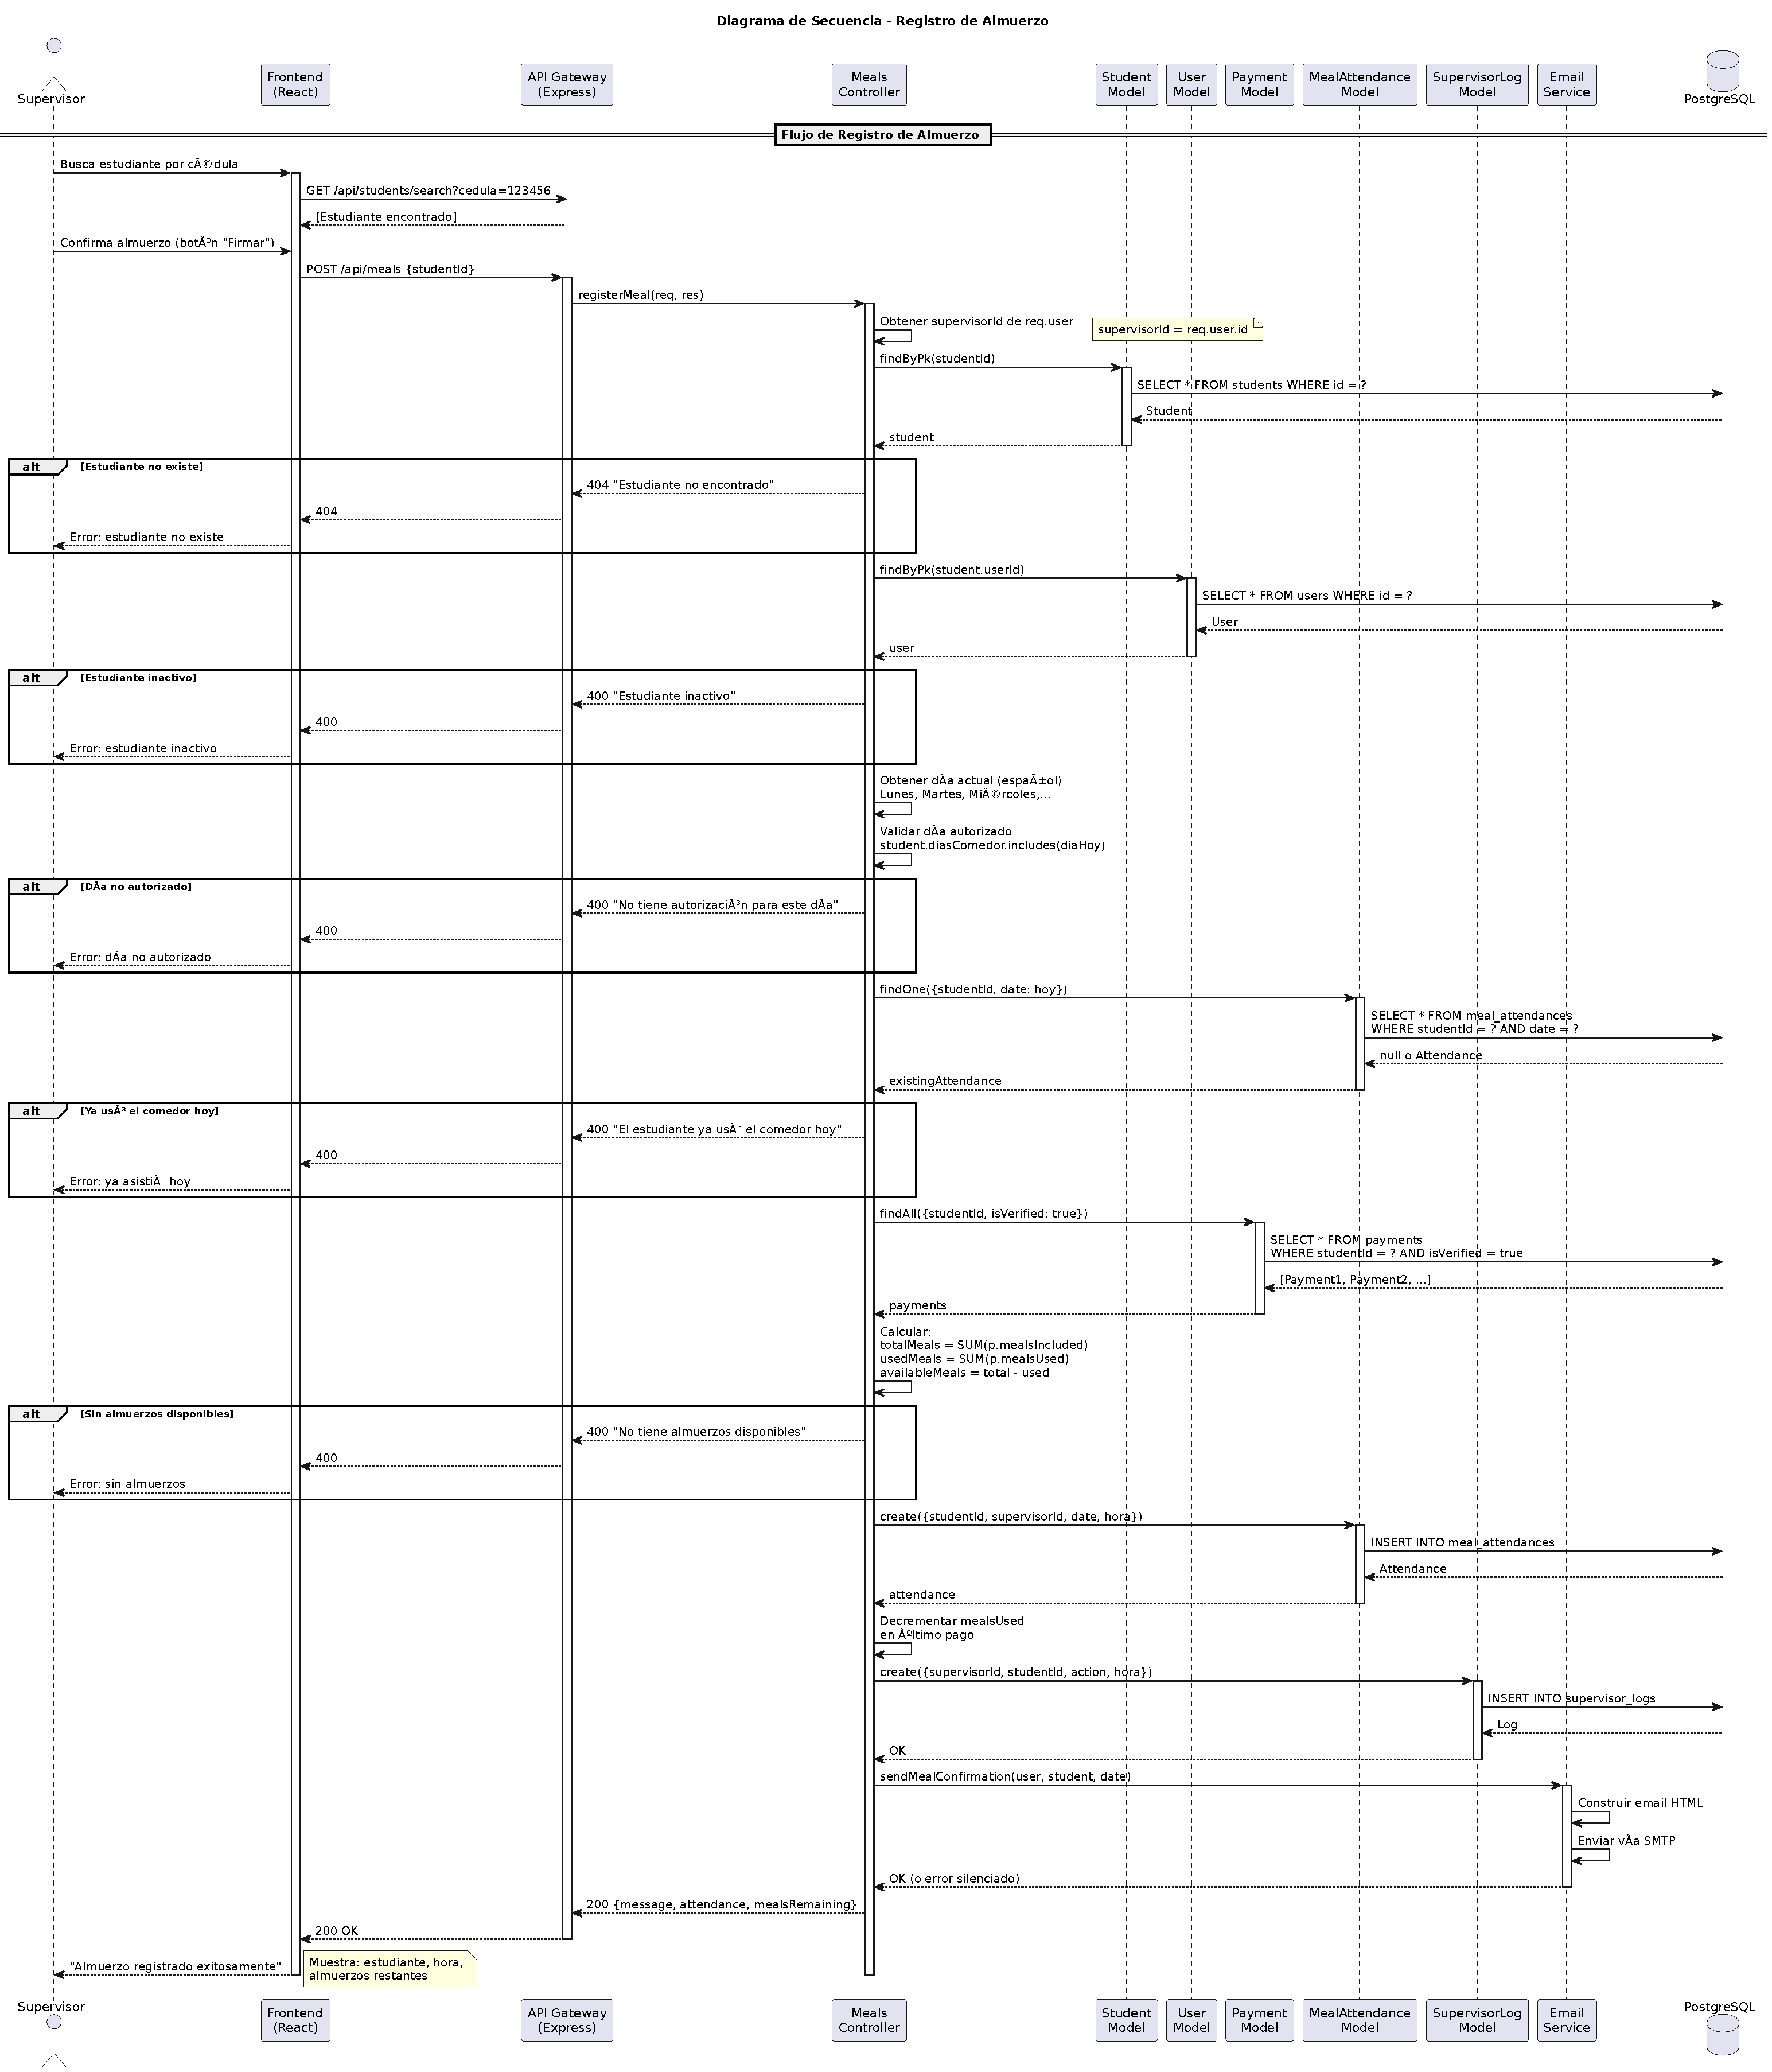
\includegraphics[width=0.92\textwidth]{figs/sequence-meal.pdf}
\caption{Diagrama de secuencia — Registro de almuerzo.}
\label{fig:seq-meal}
\end{figure}

\begin{figure}[H]
\centering
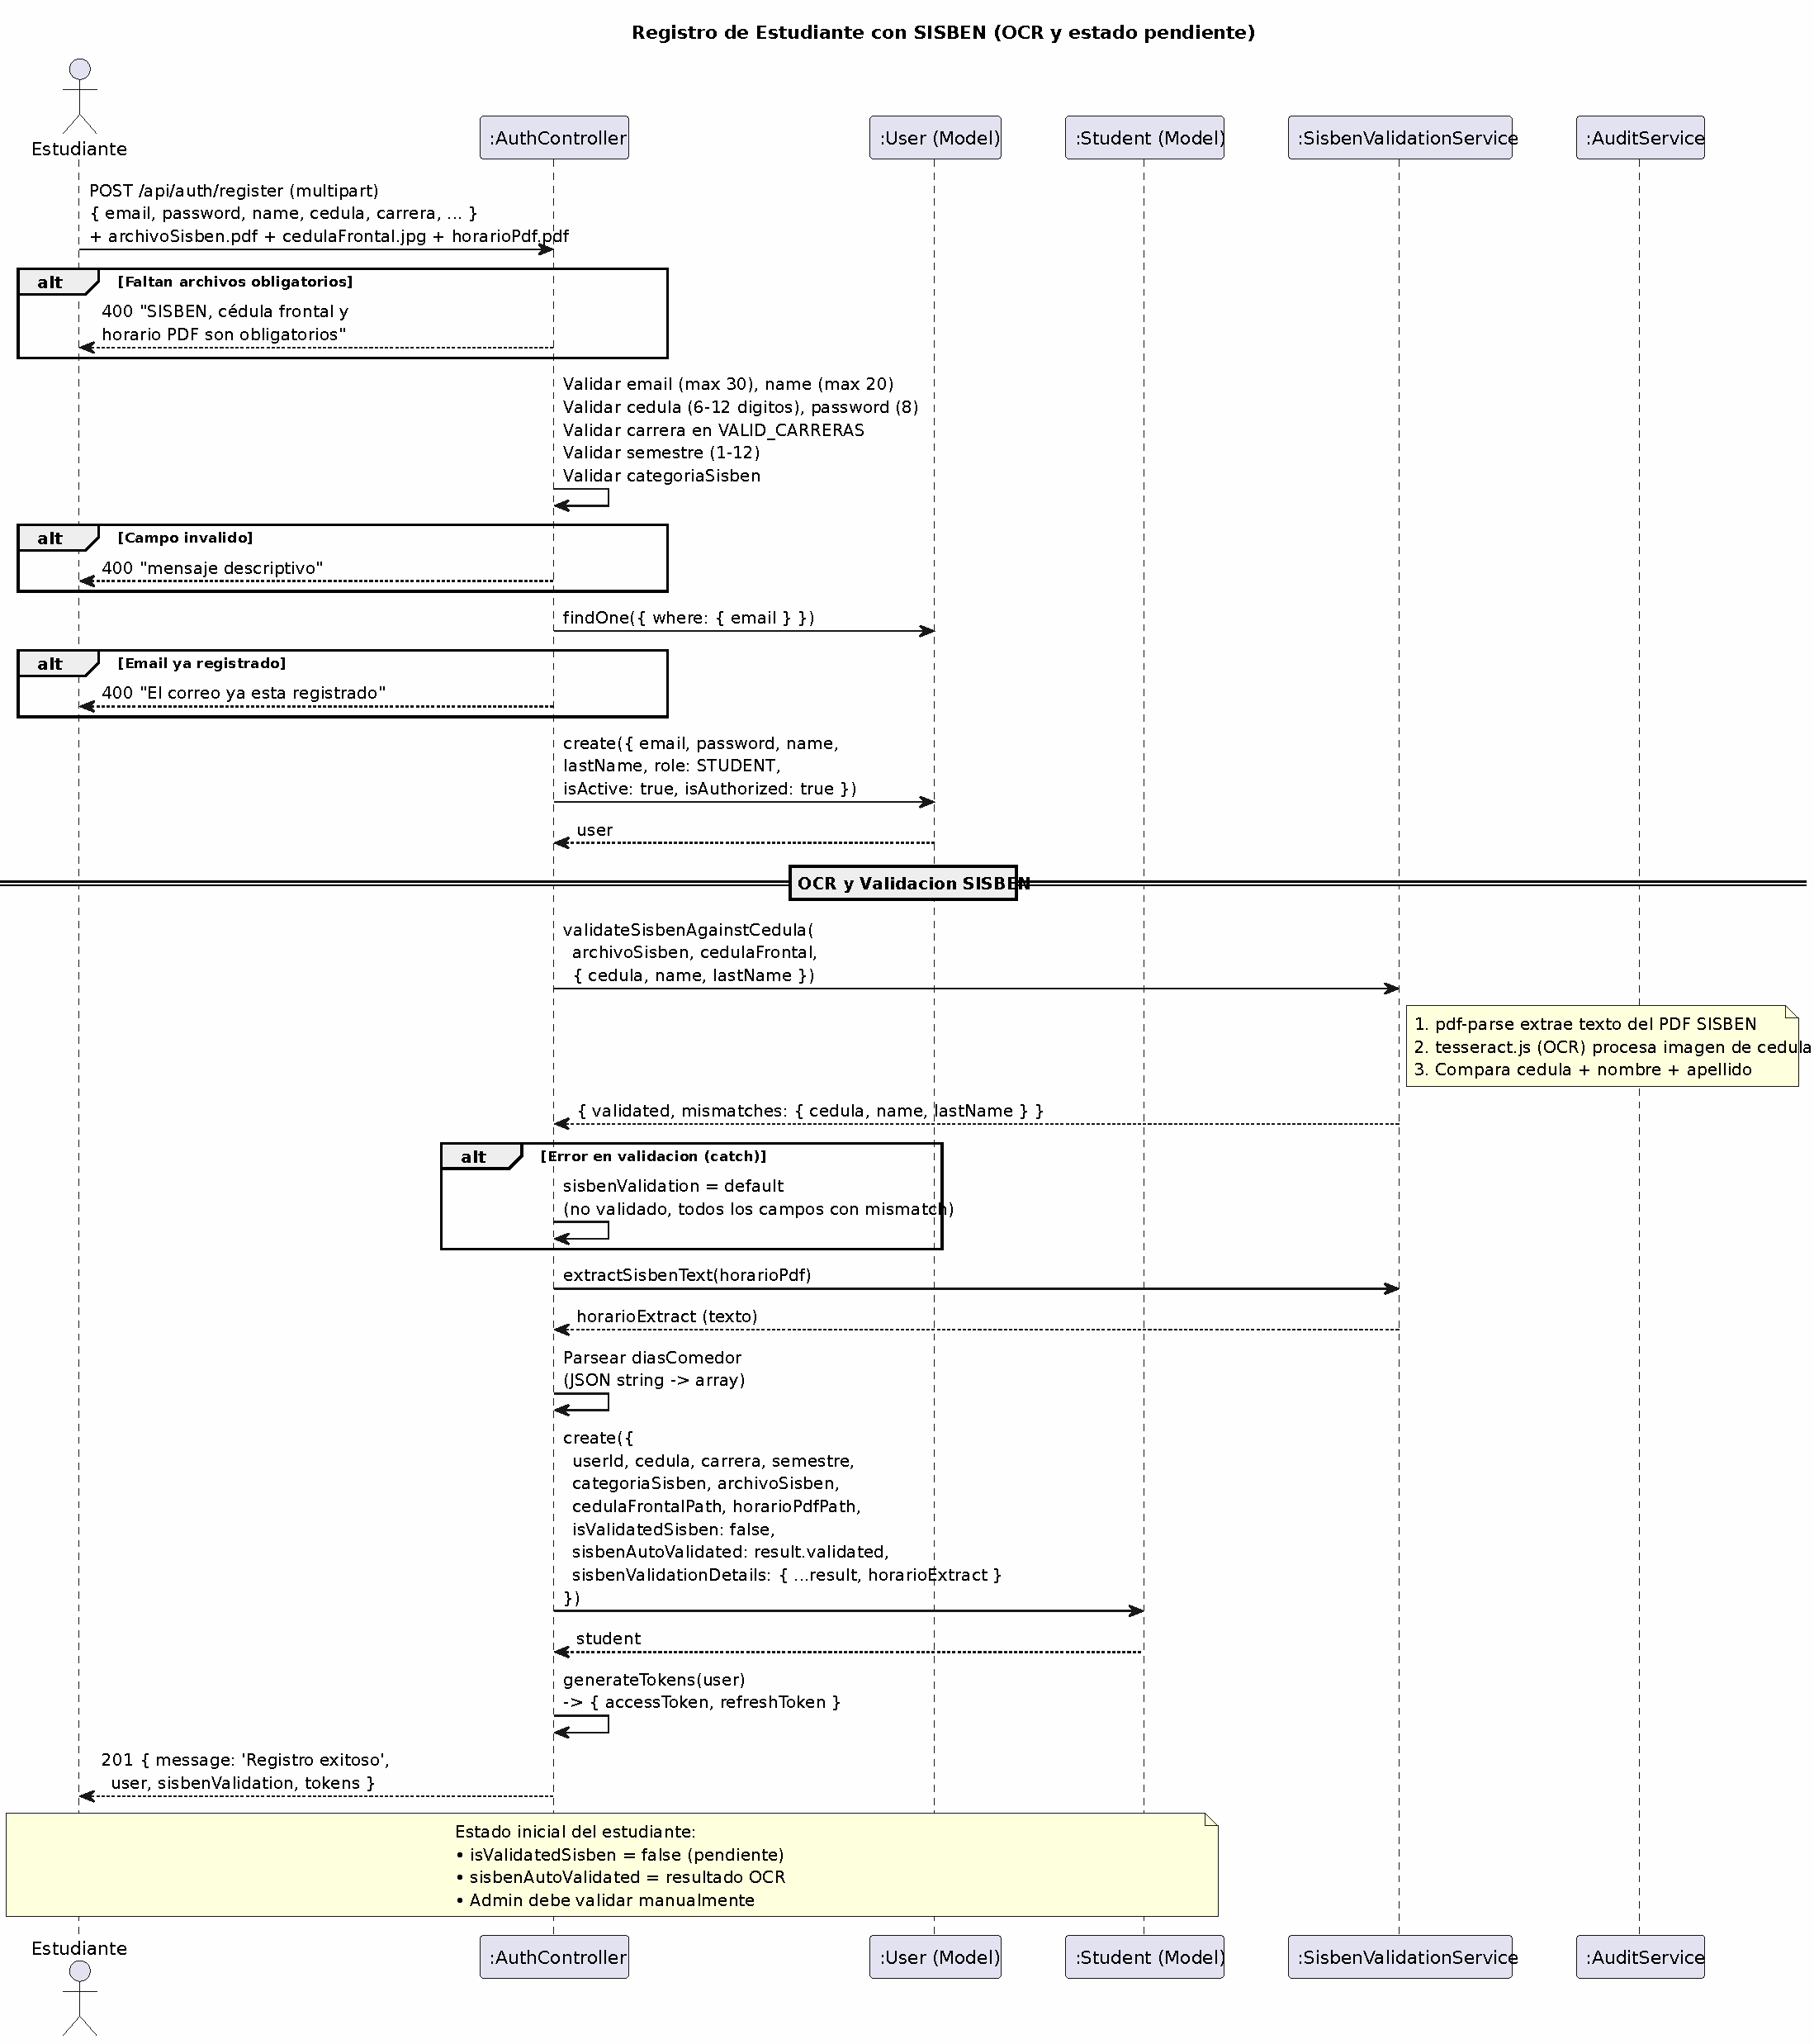
\includegraphics[width=0.92\textwidth]{figs/seq-sisben.pdf}
\caption{Diagrama de secuencia — Validación SISBÉN.}
\label{fig:seq-sisben}
\end{figure}

\subsection{Diagrama entidad–relación}
La Figura~\ref{fig:er} presenta el modelo entidad–relación. La
Tabla~\ref{tab:cardinalidades} resume las cardinalidades.

\begin{figure}[H]
\centering
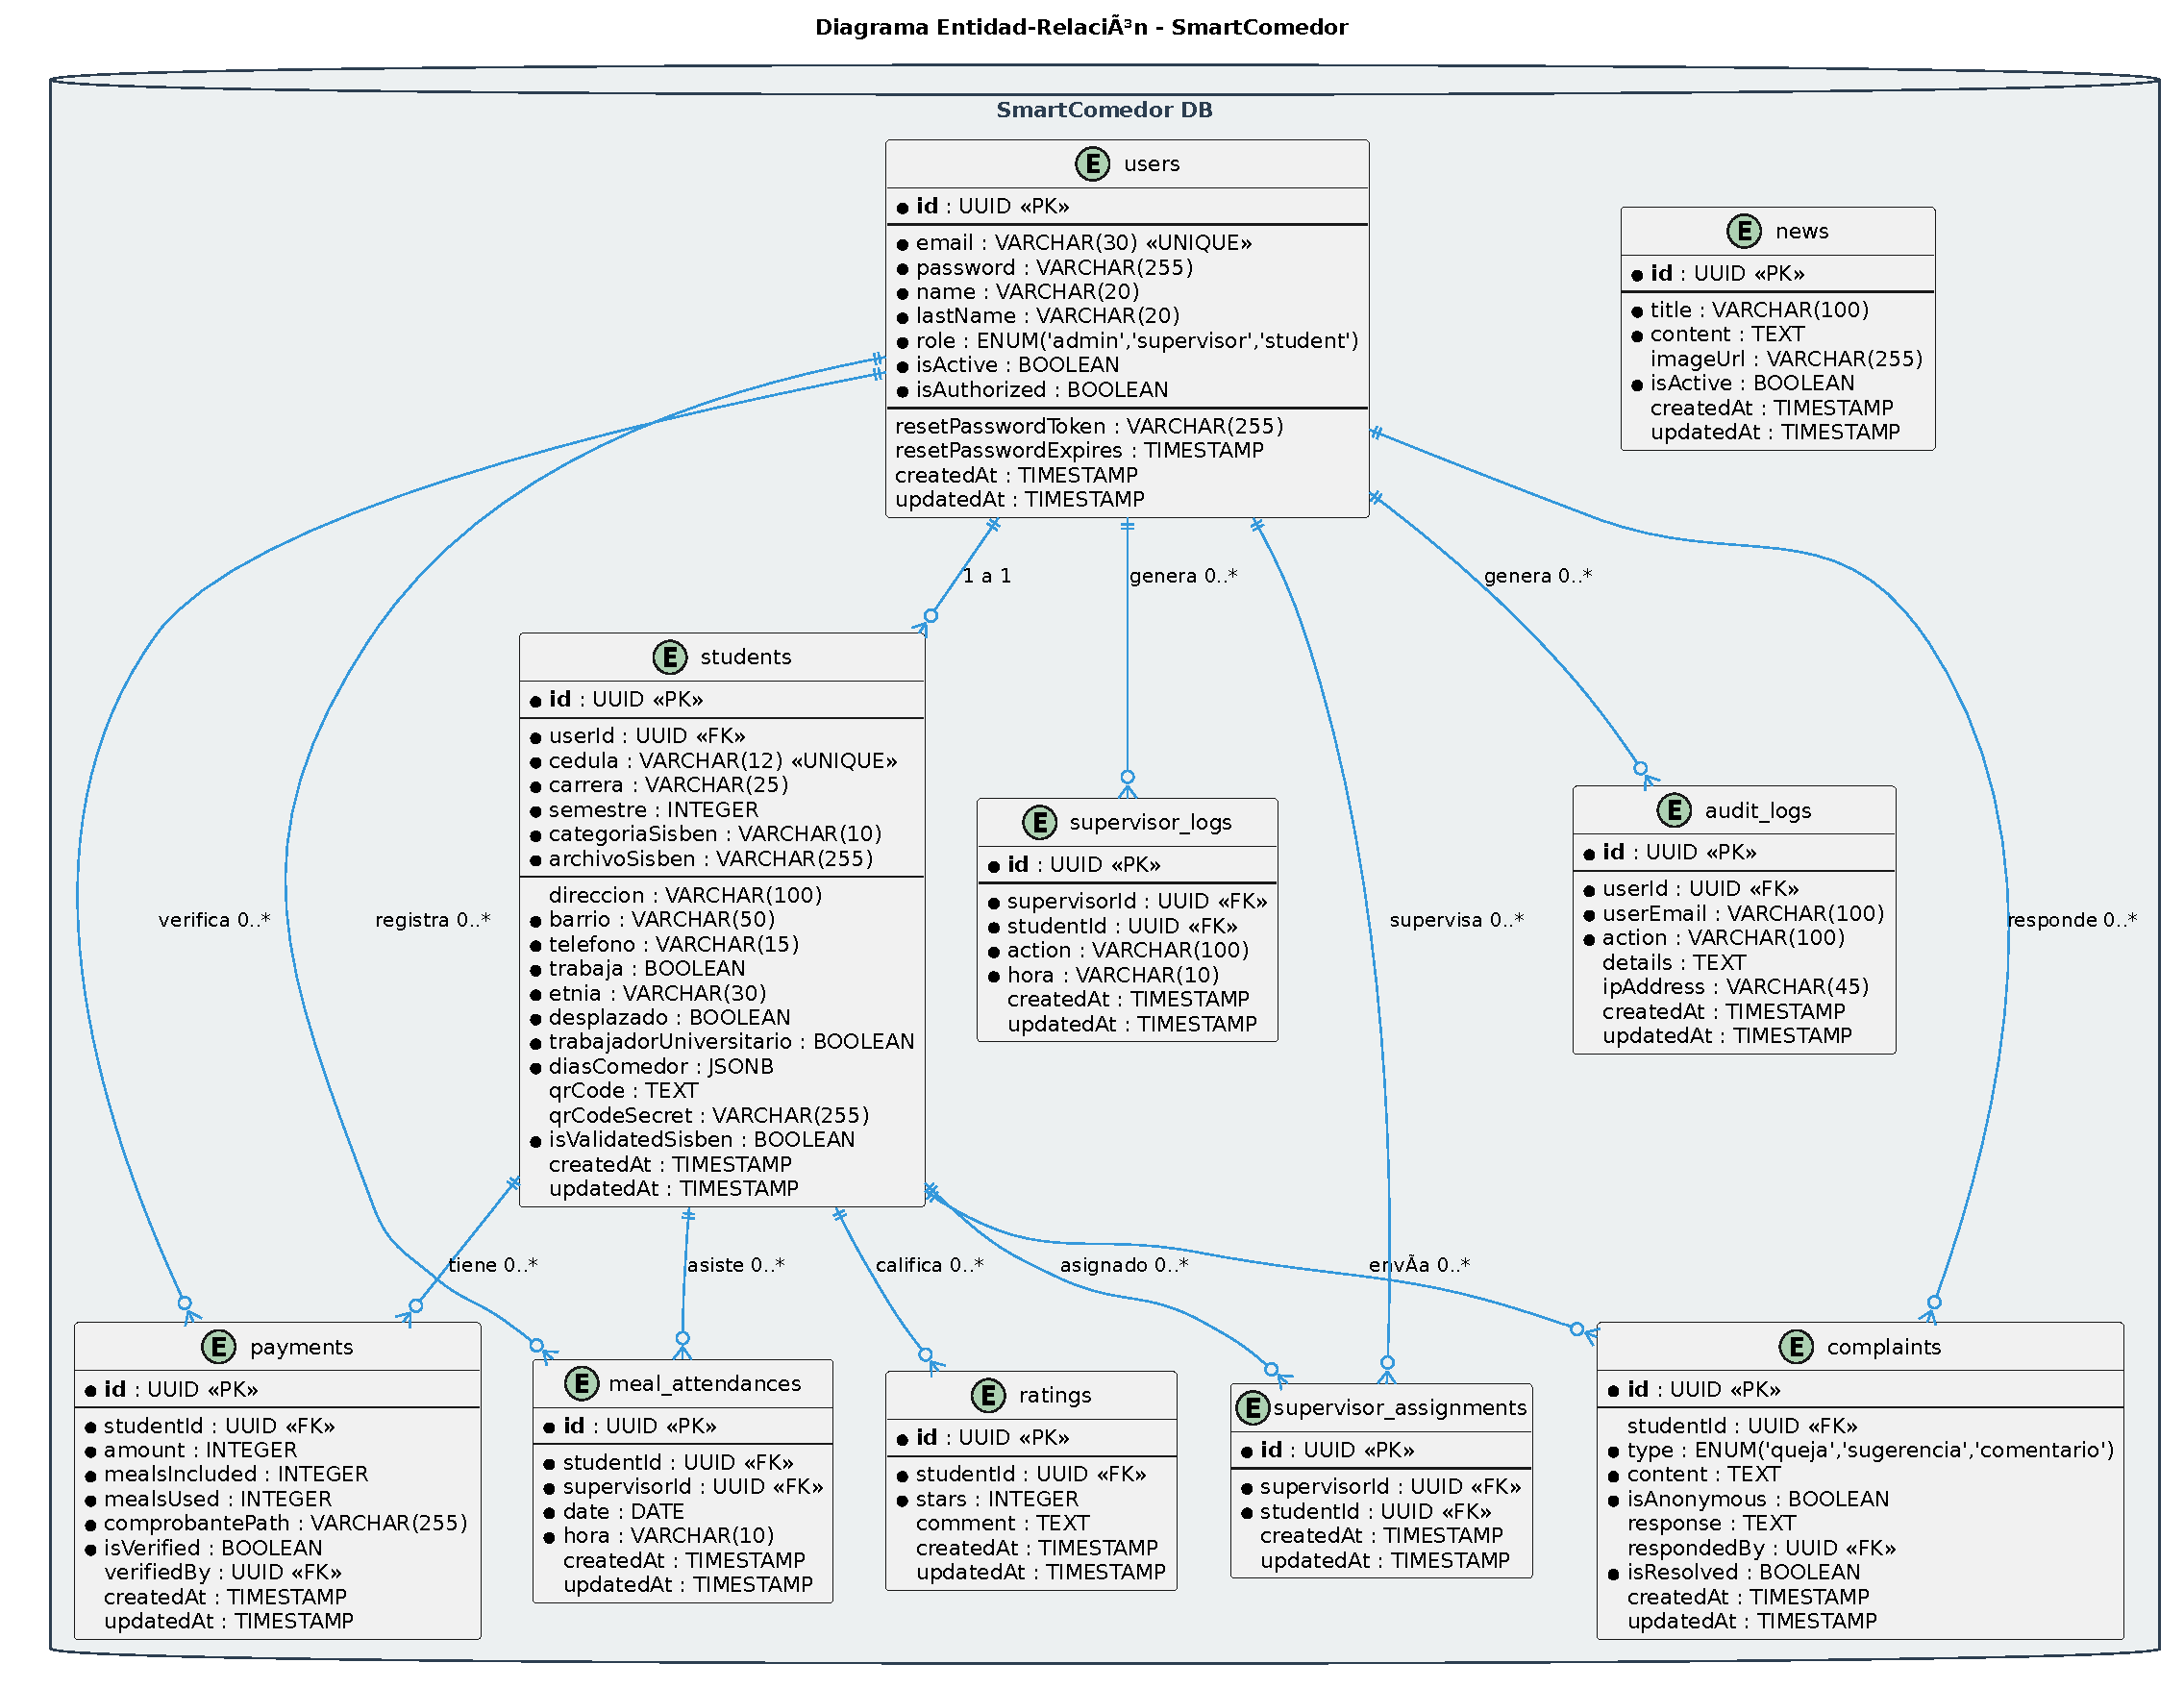
\includegraphics[width=\textwidth]{figs/er-diagram.pdf}
\caption{Diagrama entidad–relación.}
\label{fig:er}
\end{figure}

\begin{table}[H]
\centering
\caption{Cardinalidades del modelo relacional}
\label{tab:cardinalidades}
\begin{tabularx}{\textwidth}{X c}
\toprule
\textbf{Relación} & \textbf{Cardinalidad} \\
\midrule
USERS — STUDENTS & 1 : 1 \\
STUDENTS — PAYMENTS & 1 : N \\
STUDENTS — MEAL\_ATTENDANCES & 1 : N \\
USERS (supervisor) — MEAL\_ATTENDANCES & 1 : N \\
STUDENTS — RATINGS & 1 : N \\
STUDENTS — COMPLAINTS & 1 : N (0..1 del lado estudiante, anónimas) \\
STUDENTS — SUPERVISOR\_LOGS & 1 : N \\
USERS (supervisor) — STUDENTS & N : M (vía SUPERVISOR\_ASSIGNMENTS) \\
USERS — AUDIT\_LOGS & 1 : N \\
\bottomrule
\end{tabularx}
\end{table}

\subsection{Diagrama de componentes}
La Figura~\ref{fig:componentes} muestra la organización en componentes; la
Tabla~\ref{tab:componentes} describe sus responsabilidades.

\begin{figure}[H]
\centering
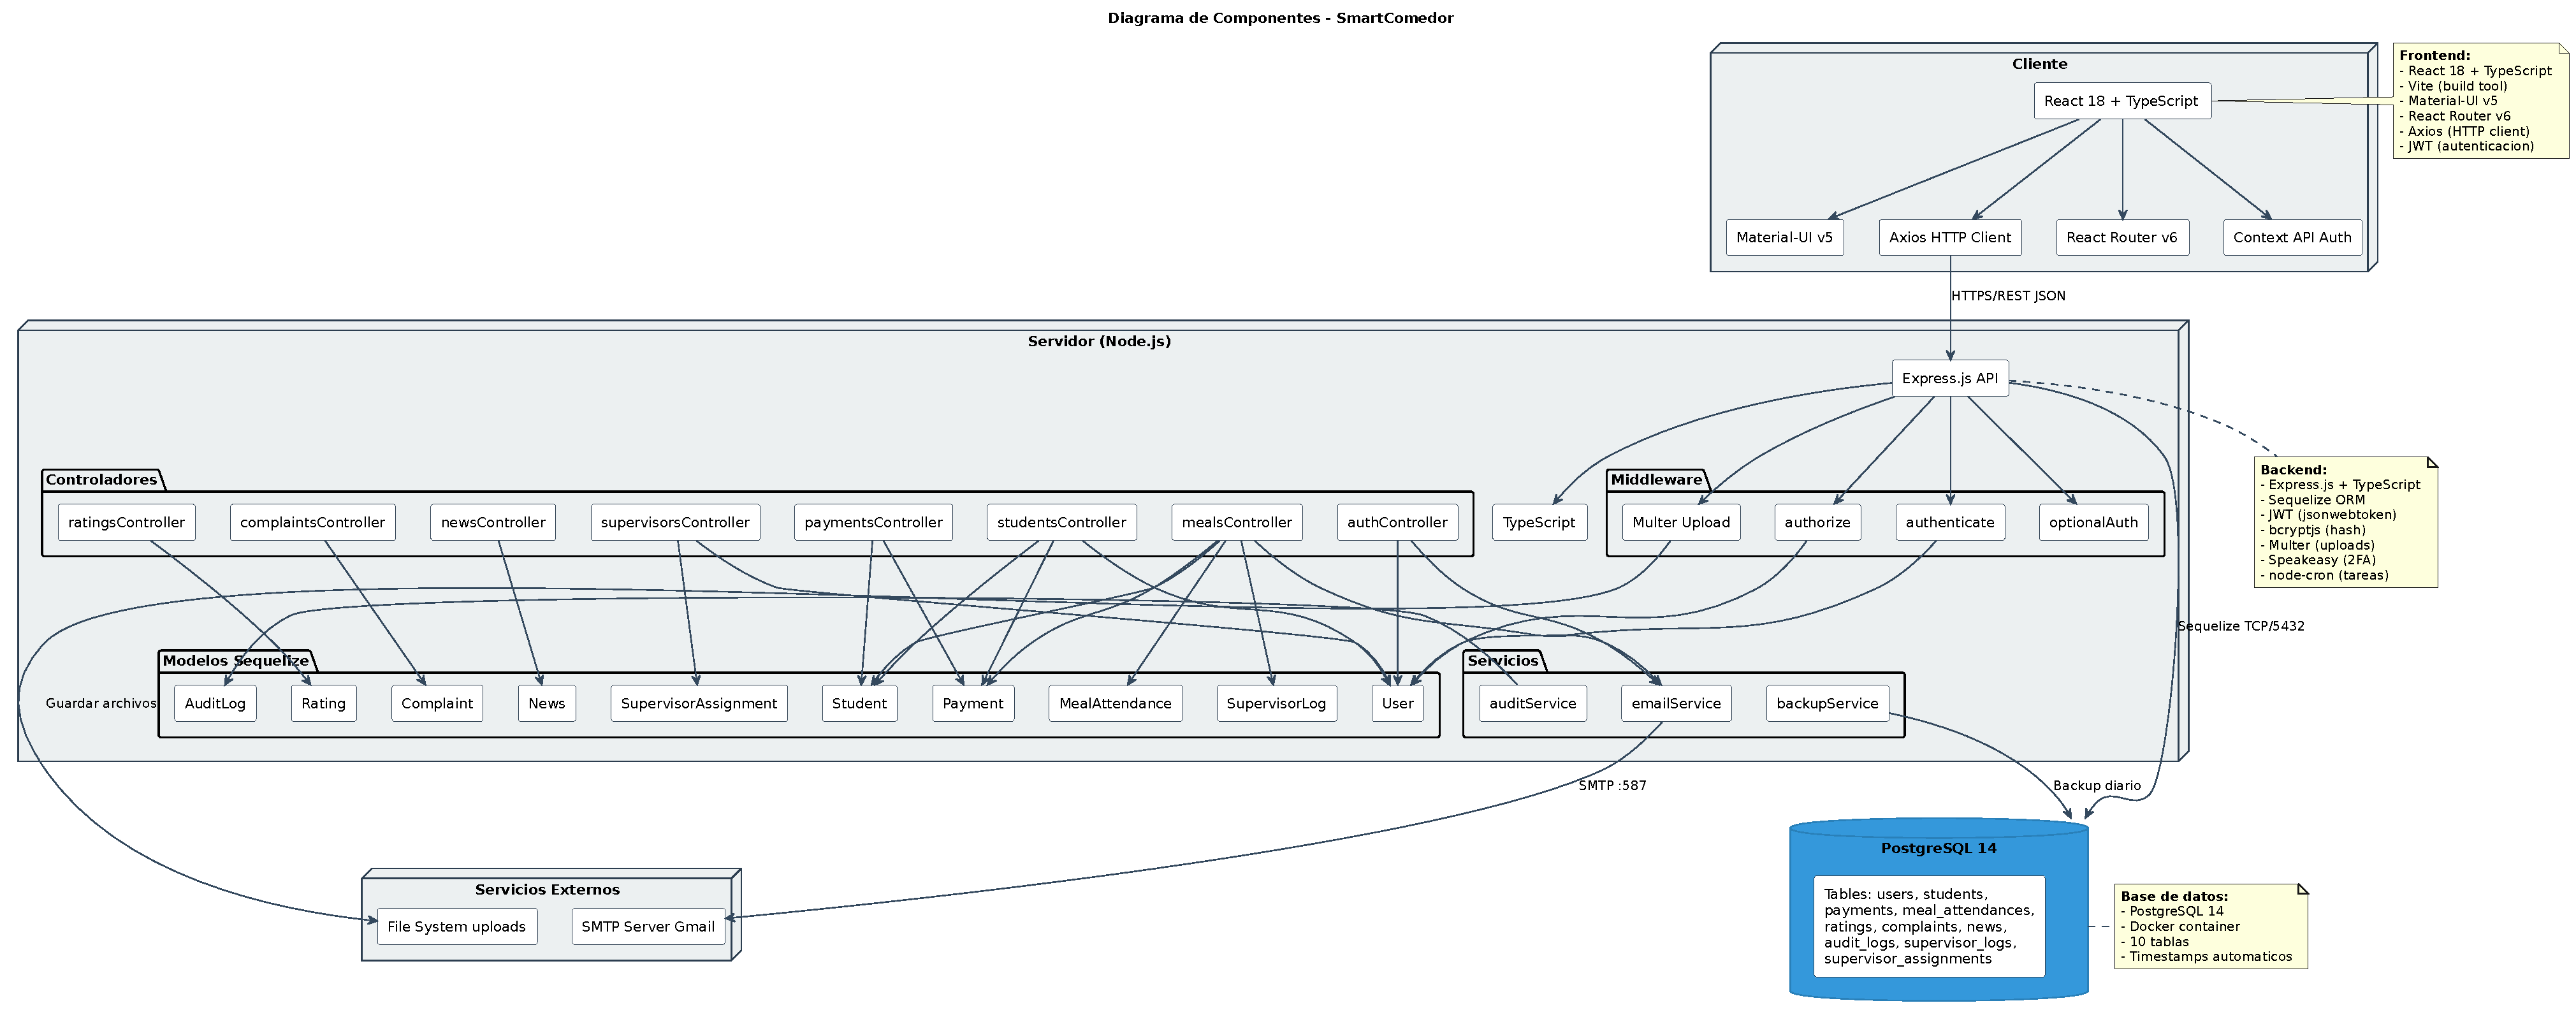
\includegraphics[width=\textwidth]{figs/components.pdf}
\caption{Diagrama de componentes.}
\label{fig:componentes}
\end{figure}

\begin{longtable}{L{0.30\textwidth} L{0.64\textwidth}}
\caption{Responsabilidades de los componentes}\label{tab:componentes}\\
\toprule
\textbf{Componente} & \textbf{Responsabilidad} \\
\midrule
\endfirsthead
\toprule
\textbf{Componente} & \textbf{Responsabilidad} \\
\midrule
\endhead
\bottomrule
\endlastfoot
Frontend SPA & Interfaz por rol, manejo de sesión (tokens), consumo de la API (axios), rutas protegidas. \\
API Express & Exposición de endpoints REST bajo \texttt{/api}, validación y orquestación de servicios. \\
Middleware Auth & \texttt{authenticate} (verifica JWT), \texttt{authorize} (rol), \texttt{optionalAuth}. \\
Middleware Upload & Recepción de archivos con multer. \\
Middleware EventAudit & Registro automático de eventos HTTP en la auditoría. \\
Controllers & Lógica de negocio por entidad. \\
EmailService & Envío de correos (recuperación de contraseña, invitaciones). \\
SisbenValidationService & Extracción de texto (PDF/OCR) y cotejo de elegibilidad. \\
AuditService & Persistencia de la bitácora de auditoría. \\
BackupService & Respaldo periódico de la base de datos. \\
CycleAutomationService & Cierre automático de ciclos y revalidación (cron). \\
Models (Sequelize) & Mapeo objeto-relacional y asociaciones. \\
PostgreSQL & Persistencia de datos. \\
\end{longtable}

% ────────────────────────────────────────────────────────────────────────────
\section{Producto del software}

\subsection{Despliegue}
El producto se despliega con Docker Compose. El Código~\ref{lst:deploy} muestra los
comandos principales.

\begin{lstlisting}[caption={Despliegue del producto},label={lst:deploy},captionpos=b]
# Variables de entorno
cp .env.example server/.env   # completar JWT_SECRET, JWT_REFRESH_SECRET, SMTP_USER, SMTP_PASS

# Desarrollo (hot-reload): Frontend :5174, Backend :3002, PostgreSQL :5433
docker compose --profile dev up --build

# Produccion (builds + nginx): Frontend :80, Backend :3002
docker compose --profile prod up --build
\end{lstlisting}

\subsection{Estructura del producto}
\begin{lstlisting}[caption={Estructura del proyecto},captionpos=b]
SmartDinningRoom/
  client/   # Frontend React + Vite (SPA por rol)
  server/   # Backend Express + Sequelize (API REST /api)
  diagrams/ # Diagramas PlantUML + SVG
  docs/     # Documentacion, diagramas e informes
  tests/    # Pruebas de sistema (seguridad, rendimiento, portabilidad)
  docker-compose.yml
  .env.example
\end{lstlisting}

\subsection{Características destacadas}
Seguridad por diseño (JWT con refresh, control de acceso por rol, 2FA TOTP, cifrado de
contraseñas, validación de filtros por lista blanca y cabeceras de seguridad);
antifraude (validación automática del SISBÉN por OCR/PDF e identificación con QR);
trazabilidad total (\texttt{audit\_logs} y \texttt{supervisor\_logs}); automatización
(importación masiva, cálculo de almuerzos, cierre de ciclos y backups programados); y
operación 24/7 (healthchecks, perfiles dev/prod y backups con retención de 30 días).

% ════════════════════════════════════════════════════════════════════════════
\part*{SEGUNDA PARTE. Pruebas del Software}
\addcontentsline{toc}{part}{SEGUNDA PARTE. Pruebas del Software}
% ════════════════════════════════════════════════════════════════════════════

\section{Introducción}
Esta parte describe el proceso de verificación y validación (V\&V) del sistema
SmartComedor \parencite{ieee829}. Las pruebas garantizan que el software cumple los
requisitos funcionales y no funcionales y que las reglas de negocio críticas
(elegibilidad SISBÉN, cálculo de almuerzos, control de asistencia, control de acceso y
auditoría) se comportan de forma correcta, segura y predecible. La estrategia combina
varios niveles: pruebas unitarias (caja negra y caja blanca), pruebas de integración
(incremental y basada en hilos), pruebas de sistema (seguridad, rendimiento, usabilidad y
portabilidad) y pruebas de aceptación \parencite{myers2011,pressman2014}. Como resumen,
la suite automatizada ejecuta \textbf{196 pruebas con 100\% de éxito} (10 suites) y una
cobertura global aproximada del \textbf{80,4\%} de sentencias medida con Jest
\parencite{jest}.

% ────────────────────────────────────────────────────────────────────────────
\section{Planificación de las pruebas}

\subsection{Objetivos de las pruebas}
\begin{table}[H]
\centering
\caption{Objetivos de las pruebas}
\label{tab:objetivos}
\begin{tabularx}{\textwidth}{c X}
\toprule
\textbf{ID} & \textbf{Objetivo} \\
\midrule
OBJ-01 & Verificar que cada requisito funcional (RF-01\,\ldots\,RF-45) está implementado y se comporta según lo especificado. \\
OBJ-02 & Verificar las reglas de negocio críticas (cálculo de almuerzos, monto mínimo, un almuerzo por día, día autorizado, disponibilidad y validación SISBÉN). \\
OBJ-03 & Verificar el control de acceso (JWT, autorización por rol y manejo de cuentas inactivas/no autorizadas). \\
OBJ-04 & Detectar defectos lo antes posible mediante pruebas automatizadas. \\
OBJ-05 & Validar atributos de calidad (seguridad, rendimiento, usabilidad, portabilidad). \\
OBJ-06 & Asegurar una cobertura de código adecuada y trazable. \\
OBJ-07 & Validar, con criterios de aceptación, la satisfacción de las necesidades del usuario. \\
\bottomrule
\end{tabularx}
\end{table}

\subsection{Alcance de las pruebas}
\textbf{Dentro del alcance:} controladores del backend; middleware de seguridad;
servicios (validación SISBÉN, auditoría); flujos de integración entre módulos; atributos
de calidad (cabeceras de seguridad, control de acceso, carga/estrés, portabilidad
cross-browser y usabilidad/accesibilidad básica). \textbf{Fuera del alcance (o cubierto
indirectamente):} pruebas exhaustivas de componentes React; pruebas de proveedores
externos (SMTP, infraestructura de BrowserStack); y \emph{penetration testing} avanzado
más allá del escaneo automatizado (OWASP ZAP) y JMeter \parencite{owasp2021}.

\subsection{Estrategias de pruebas}
La Tabla~\ref{tab:estrategias} resume el mapeo de niveles, técnicas y herramientas.

\begin{longtable}{L{0.20\textwidth} L{0.34\textwidth} L{0.38\textwidth}}
\caption{Estrategias de pruebas por nivel}\label{tab:estrategias}\\
\toprule
\textbf{Nivel} & \textbf{Técnica} & \textbf{Herramienta / ubicación} \\
\midrule
\endfirsthead
\toprule
\textbf{Nivel} & \textbf{Técnica} & \textbf{Herramienta / ubicación} \\
\midrule
\endhead
\bottomrule
\endlastfoot
Unitario & Caja negra (equivalencia, valores límite) + caja blanca (caminos) & Jest + ts-jest (\texttt{server/src/tests/unit/}) \\
Integración & Incremental (bottom-up) & Jest (\texttt{integration/incremental.test.ts}) \\
Integración & Basada en hilos (por actor) & Jest (\texttt{integration/threads.test.ts}) \\
Sistema — Seguridad & Cabeceras, control de acceso, escaneo & Playwright + OWASP ZAP + JMeter \\
Sistema — Rendimiento & Carga y estrés & Apache JMeter (\texttt{tests/security/jmeter/}) \\
Sistema — Portabilidad & Cross-browser & Playwright + BrowserStack \\
Sistema — Usabilidad & Inspección heurística + accesibilidad & Playwright + revisión MUI \\
Aceptación & Escenarios de usuario (Gherkin) & Manual / Playwright \\
\end{longtable}

Las técnicas de diseño empleadas son: \textbf{particiones de equivalencia} (clases
válidas e inválidas), \textbf{análisis de valores límite} (fronteras de rangos),
\textbf{cobertura de caminos} (grafo de flujo) y \textbf{pruebas basadas en estado}
\parencite{myers2011,beizer1990}.

\subsection{Ambiente de pruebas}\label{sec:ambiente}
La Tabla~\ref{tab:ambiente} describe el ambiente. Las pruebas unitarias y de integración
emplean una base de datos simulada en memoria (mocks), lo que permite ejecutarlas sin
PostgreSQL real, de forma determinista y veloz.

\begin{table}[H]
\centering
\caption{Ambiente de pruebas}
\label{tab:ambiente}
\begin{tabularx}{\textwidth}{L{0.34\textwidth} X}
\toprule
\textbf{Elemento} & \textbf{Versión / detalle} \\
\midrule
Node.js & 20+ (probado con v22) \\
Framework de pruebas & Jest 29 + ts-jest 29 \\
Lenguaje & TypeScript 5 \\
BD en unitarias/integración & Mock en memoria (sin PostgreSQL real) \\
Pruebas de sistema & Docker (JMeter), Playwright 1.44, BrowserStack, OWASP ZAP \\
\bottomrule
\end{tabularx}
\end{table}

\begin{lstlisting}[caption={Scripts de ejecución (backend)},captionpos=b]
cd server
npm test                  # toda la suite
npm run test:unit         # solo unitarias
npm run test:integration  # solo integracion
npm run test:coverage     # con reporte de cobertura
\end{lstlisting}

% ────────────────────────────────────────────────────────────────────────────
\section{Pruebas unitarias}

\subsection{Análisis de las pruebas}
Las pruebas unitarias aíslan la unidad bajo prueba (controlador, middleware o servicio)
mediante mocks de los modelos Sequelize, de \texttt{jsonwebtoken}, de \texttt{bcrypt}, de
\texttt{nodemailer} y del sistema de archivos. Se priorizaron las unidades de mayor
riesgo: \texttt{authController} (seguridad de acceso, tokens, recuperación de contraseña,
2FA), \texttt{middleware/auth} (control de acceso), \texttt{paymentsController} (cálculo
monetario), \texttt{mealsController} (reglas de asistencia), \texttt{studentsController}
(CRUD, importación, SISBÉN) y los servicios de validación. La
Tabla~\ref{tab:distribucion} presenta la distribución de casos por suite.

\begin{table}[H]
\centering
\caption{Distribución de casos por suite}
\label{tab:distribucion}
\begin{tabularx}{\textwidth}{X c}
\toprule
\textbf{Suite (archivo)} & \textbf{Casos \texttt{it()}} \\
\midrule
unit/authController.test.ts & 59 \\
unit/studentsController.test.ts & 28 \\
unit/paymentsController.test.ts & 21 \\
unit/supervisorsController.test.ts & 19 \\
unit/ratingsComplaintsNews.test.ts & 17 \\
unit/middleware.test.ts & 15 \\
unit/mealsController.test.ts & 13 \\
unit/sisbenValidationService.test.ts & 6 \\
integration/incremental.test.ts & 16 \\
integration/threads.test.ts & 8 \\
\midrule
\textbf{Total} & \textbf{202 declarados (196 ejecutados/aprobados)} \\
\bottomrule
\end{tabularx}
\end{table}

\subsection{Catálogo detallado de casos de prueba}
% Generado por gen_pruebas.py

A continuacion se presenta el catalogo completo de los casos de prueba automatizados, extraido directamente del codigo fuente de las suites (\texttt{server/src/tests/}). Cada caso corresponde a un bloque \texttt{it()} ejecutable; la columna \emph{Contexto} indica el bloque \texttt{describe()} que lo agrupa.


El catalogo agrupa \textbf{196} casos declarados en las diez suites.


\subsubsection{AuthController (\texttt{unit/authController.test.ts})}
La suite \texttt{unit/authController.test.ts} contiene 59 casos de prueba (Tabla~\ref{tab:cat-tc-auth}).
\begin{longtable}{l L{0.30\textwidth} L{0.40\textwidth}}
\caption{Casos de prueba --- AuthController}\label{tab:cat-tc-auth}\\
\toprule \textbf{ID} & \textbf{Contexto} & \textbf{Caso de prueba} \\ \midrule
\endfirsthead
\toprule \textbf{ID} & \textbf{Contexto} & \textbf{Caso de prueba} \\ \midrule
\endhead \bottomrule \endlastfoot
TC-AUTH-001 & authController > login > Caja Negra - Clases de Equivalencia & TC-LOGIN-001: Login exitoso como administrador \\
TC-AUTH-002 & authController > login > Caja Negra - Clases de Equivalencia & TC-LOGIN-002: Login exitoso como estudiante \\
TC-AUTH-003 & authController > login > Caja Negra - Clases de Equivalencia & TC-LOGIN-003: Login exitoso como supervisor autorizado \\
TC-AUTH-004 & authController > login > Caja Negra - Clases de Equivalencia & TC-LOGIN-004: Error 400 - Campos requeridos faltantes (sin email) \\
TC-AUTH-005 & authController > login > Caja Negra - Clases de Equivalencia & TC-LOGIN-005: Error 400 - Campos requeridos faltantes (sin password) \\
TC-AUTH-006 & authController > login > Caja Negra - Clases de Equivalencia & TC-LOGIN-006: Error 400 - Campos requeridos faltantes (sin role) \\
TC-AUTH-007 & authController > login > Caja Negra - Clases de Equivalencia & TC-LOGIN-007: Error 401 - Usuario no existe \\
TC-AUTH-008 & authController > login > Caja Negra - Clases de Equivalencia & TC-LOGIN-008: Error 401 - Contraseña incorrecta \\
TC-AUTH-009 & authController > login > Caja Negra - Clases de Equivalencia & TC-LOGIN-009: Error 401 - Usuario inactivo \\
TC-AUTH-010 & authController > login > Caja Negra - Clases de Equivalencia & TC-LOGIN-010: Error 403 - Rol no coincide (student intenta como admin) \\
TC-AUTH-011 & authController > login > Caja Negra - Clases de Equivalencia & TC-LOGIN-011: Error 403 - Admin no autorizado (isAuthorized=false) \\
TC-AUTH-012 & authController > login > Caja Negra - Clases de Equivalencia & TC-LOGIN-012: Error 403 - Supervisor no autorizado (isAuthorized=false) \\
TC-AUTH-013 & authController > login > Caja Negra - Clases de Equivalencia & TC-LOGIN-013: Error 500 - Excepción del servidor \\
TC-AUTH-014 & authController > login > Camino Básico - Cobertura de Caminos (Grafo de Flujo) & Camino 1: Campos faltantes -> 400 \\
TC-AUTH-015 & authController > login > Camino Básico - Cobertura de Caminos (Grafo de Flujo) & Camino 2: Campos OK -> Usuario no existe -> 401 \\
TC-AUTH-016 & authController > login > Camino Básico - Cobertura de Caminos (Grafo de Flujo) & Camino 3: Campos OK -> Usuario existe -> Contraseña incorrecta -> 401 \\
TC-AUTH-017 & authController > login > Camino Básico - Cobertura de Caminos (Grafo de Flujo) & Camino 4: Campos OK -> Usuario -> Pass OK -> Inactivo -> 401 \\
TC-AUTH-018 & authController > login > Camino Básico - Cobertura de Caminos (Grafo de Flujo) & Camino 5: Campos OK -> Usuario -> Pass OK -> Activo -> Rol incorrecto -> 403 \\
TC-AUTH-019 & authController > login > Camino Básico - Cobertura de Caminos (Grafo de Flujo) & Camino 6: Camino completo hasta no autorizado -> 403 \\
TC-AUTH-020 & authController > login > Camino Básico - Cobertura de Caminos (Grafo de Flujo) & Camino 7: Camino completo exitoso -> 200 \\
TC-AUTH-021 & authController > register > Valores Límite - Campos con restricciones & VL-EMAIL-001: Email de exactamente 30 caracteres - válido \\
TC-AUTH-022 & authController > register > Valores Límite - Campos con restricciones & VL-CEDULA-001: Cédula de 6 dígitos - válido (mínimo) \\
TC-AUTH-023 & authController > register > Valores Límite - Campos con restricciones & VL-CEDULA-002: Cédula de 12 dígitos - válido (máximo) \\
TC-AUTH-024 & authController > register > Valores Límite - Campos con restricciones & VL-CEDULA-003: Cédula de 5 dígitos - inválido (debajo del mínimo) \\
TC-AUTH-025 & authController > register > Valores Límite - Campos con restricciones & VL-NOMBRE-001: Nombre de 20 caracteres - válido \\
TC-AUTH-026 & authController > register > Valores Límite - Campos con restricciones & VL-NOMBRE-002: Nombre de 21 caracteres - inválido \\
TC-AUTH-027 & authController > register > Caja Negra - Clases de Equivalencia & TC-REG-001: Registro exitoso con todos los campos válidos \\
TC-AUTH-028 & authController > register > Caja Negra - Clases de Equivalencia & TC-REG-002: Error 400 - Archivo SISBEN faltante \\
TC-AUTH-029 & authController > register > Caja Negra - Clases de Equivalencia & TC-REG-003: Error 400 - Email ya registrado \\
TC-AUTH-030 & authController > register > Caja Negra - Clases de Equivalencia & TC-REG-004: Parseo correcto de diasComedor desde string JSON \\
TC-AUTH-031 & authController > refreshToken & TC-REFRESH-001: Refresh exitoso con token válido \\
TC-AUTH-032 & authController > refreshToken & TC-REFRESH-002: Error 400 - Token faltante \\
TC-AUTH-033 & authController > refreshToken & TC-REFRESH-003: Error 401 - Token JWT inválido \\
TC-AUTH-034 & authController > refreshToken & TC-REFRESH-004: Error 401 - Usuario no encontrado \\
TC-AUTH-035 & authController > refreshToken & TC-REFRESH-005: Error 401 - Usuario inactivo \\
TC-AUTH-036 & authController > getProfile & TC-PROFILE-001: Obtener perfil exitoso \\
TC-AUTH-037 & authController > getProfile & TC-PROFILE-002: Error 404 - Usuario no encontrado \\
TC-AUTH-038 & authController > updateProfile & TC-UPDATE-001: Actualización de perfil exitosa \\
TC-AUTH-039 & authController > updateProfile & TC-UPDATE-002: Error 404 - Usuario no encontrado \\
TC-AUTH-040 & authController > forgotPassword & TC-FORGOT-001: Email enviado cuando usuario existe \\
TC-AUTH-041 & authController > forgotPassword & TC-FORGOT-002: Error 400 - Email faltante \\
TC-AUTH-042 & authController > forgotPassword & TC-FORGOT-003: Mensaje genérico cuando usuario NO existe (seguridad) \\
TC-AUTH-043 & authController > resetPassword & TC-RESET-001: Contraseña restablecida exitosamente \\
TC-AUTH-044 & authController > resetPassword & TC-RESET-002: Error 400 - Token faltante \\
TC-AUTH-045 & authController > resetPassword & TC-RESET-003: Error 400 - Contraseña nueva faltante \\
TC-AUTH-046 & authController > resetPassword & TC-RESET-004: Error 400 - Contraseña NO tiene exactamente 8 caracteres (7) \\
TC-AUTH-047 & authController > resetPassword & TC-RESET-005: Error 400 - Contraseña NO tiene exactamente 8 caracteres (9) \\
TC-AUTH-048 & authController > resetPassword & TC-RESET-006: Error 400 - Token inválido o expirado \\
TC-AUTH-049 & authController > changePassword & TC-CHANGE-001: Contraseña cambiada exitosamente \\
TC-AUTH-050 & authController > changePassword & TC-CHANGE-002: Error 404 - Usuario no encontrado \\
TC-AUTH-051 & authController > changePassword & TC-CHANGE-003: Error 400 - Contraseña actual incorrecta \\
TC-AUTH-052 & authController > setupTwoFactor & TC-2FA-SETUP-001: Configuración 2FA exitosa para estudiante \\
TC-AUTH-053 & authController > setupTwoFactor & TC-2FA-SETUP-002: Error 404 - Usuario no encontrado \\
TC-AUTH-054 & authController > setupTwoFactor & TC-2FA-SETUP-003: Error 400 - Solo estudiantes (admin no puede) \\
TC-AUTH-055 & authController > verifyTwoFactor & TC-2FA-VERIFY-001: Verificación 2FA exitosa \\
TC-AUTH-056 & authController > verifyTwoFactor & TC-2FA-VERIFY-002: Error 400 - Token 2FA faltante \\
TC-AUTH-057 & authController > verifyTwoFactor & TC-2FA-VERIFY-003: Error 404 - Usuario no encontrado \\
TC-AUTH-058 & authController > verifyTwoFactor & TC-2FA-VERIFY-004: Error 400 - 2FA no configurado previamente \\
TC-AUTH-059 & authController > verifyTwoFactor & TC-2FA-VERIFY-005: Error 400 - Código TOTP inválido \\
\end{longtable}

\subsubsection{StudentsController (\texttt{unit/studentsController.test.ts})}
La suite \texttt{unit/studentsController.test.ts} contiene 28 casos de prueba (Tabla~\ref{tab:cat-tc-stu}).
\begin{longtable}{l L{0.30\textwidth} L{0.40\textwidth}}
\caption{Casos de prueba --- StudentsController}\label{tab:cat-tc-stu}\\
\toprule \textbf{ID} & \textbf{Contexto} & \textbf{Caso de prueba} \\ \midrule
\endfirsthead
\toprule \textbf{ID} & \textbf{Contexto} & \textbf{Caso de prueba} \\ \midrule
\endhead \bottomrule \endlastfoot
TC-STU-001 & studentsController > getStudents & TC-GET-STU-001: Obtener lista de estudiantes exitosamente \\
TC-STU-002 & studentsController > getStudents & TC-GET-STU-002: Paginación correcta \\
TC-STU-003 & studentsController > getStudents & TC-GET-STU-003: Búsqueda por texto (search) \\
TC-STU-004 & studentsController > getStudentById & TC-BY-ID-001: Obtener estudiante por ID exitosamente \\
TC-STU-005 & studentsController > getStudentById & TC-BY-ID-002: Error 404 - Estudiante no encontrado \\
TC-STU-006 & studentsController > getStudentById & TC-BY-ID-003: Sin pagos verificados - availableMeals = 0 \\
TC-STU-007 & studentsController > createStudent > Valores Límite & VL-CEDULA: Cédula de 6 dígitos (mínimo) \\
TC-STU-008 & studentsController > createStudent > Valores Límite & VL-CEDULA: Cédula de 12 dígitos (máximo) \\
TC-STU-009 & studentsController > createStudent > Valores Límite & VL-NOMBRE: Nombre de 20 caracteres (máximo) \\
TC-STU-010 & studentsController > createStudent > Valores Límite & VL-CARRERA: Carrera de 25 caracteres (máximo) \\
TC-STU-011 & studentsController > createStudent > Caja Negra - Clases de Equivalencia & TC-CREATE-001: Creación exitosa con datos válidos \\
TC-STU-012 & studentsController > createStudent > Caja Negra - Clases de Equivalencia & TC-CREATE-002: Error 400 - Email ya registrado \\
TC-STU-013 & studentsController > createStudent > Caja Negra - Clases de Equivalencia & TC-CREATE-003: DiasComedor se asigna correctamente \\
TC-STU-014 & studentsController > updateStudent & TC-UPDATE-001: Actualización exitosa \\
TC-STU-015 & studentsController > updateStudent & TC-UPDATE-002: Error 404 - Estudiante no encontrado \\
TC-STU-016 & studentsController > updateStudent & TC-UPDATE-003: Error 404 - Usuario no es estudiante (es admin) \\
TC-STU-017 & studentsController > deleteStudent & TC-DELETE-001: Deshabilitación exitosa (soft delete) \\
TC-STU-018 & studentsController > deleteStudent & TC-DELETE-002: Error 404 - Estudiante no encontrado \\
TC-STU-019 & studentsController > validateSisben & TC-SISBEN-001: Validación exitosa - todos los datos coinciden \\
TC-STU-020 & studentsController > validateSisben & TC-SISBEN-002: Validación fallida - cédula no coincide \\
TC-STU-021 & studentsController > validateSisben & TC-SISBEN-003: Error 404 - Estudiante no encontrado \\
TC-STU-022 & studentsController > getAvailableMeals & TC-MEALS-001: Calcular almuerzos disponibles correctamente \\
TC-STU-023 & studentsController > getAvailableMeals & TC-MEALS-002: Error 404 - Estudiante no encontrado \\
TC-STU-024 & studentsController > searchStudents & TC-SEARCH-001: Búsqueda por cédula \\
TC-STU-025 & studentsController > searchStudents & TC-SEARCH-002: Búsqueda sin filtros retorna todos \\
TC-STU-026 & studentsController > importStudentsFromExcel & TC-IMPORT-001: Error 400 - No se envió archivo \\
TC-STU-027 & studentsController > importStudentsFromExcel & TC-IMPORT-002: Importar archivo Excel correctamente \\
TC-STU-028 & studentsController > importStudentsFromExcel & TC-IMPORT-003: Actualizar estudiante existente con pago \\
\end{longtable}

\subsubsection{PaymentsController (\texttt{unit/paymentsController.test.ts})}
La suite \texttt{unit/paymentsController.test.ts} contiene 21 casos de prueba (Tabla~\ref{tab:cat-tc-pay}).
\begin{longtable}{l L{0.30\textwidth} L{0.40\textwidth}}
\caption{Casos de prueba --- PaymentsController}\label{tab:cat-tc-pay}\\
\toprule \textbf{ID} & \textbf{Contexto} & \textbf{Caso de prueba} \\ \midrule
\endfirsthead
\toprule \textbf{ID} & \textbf{Contexto} & \textbf{Caso de prueba} \\ \midrule
\endhead \bottomrule \endlastfoot
TC-PAY-001 & paymentsController > createPayment > Valores Límite - Monto mínimo de 2000 (1 almuerzo) & VL-MONTO-001: Monto exactamente 2000 = 1 almuerzo \\
TC-PAY-002 & paymentsController > createPayment > Valores Límite - Monto mínimo de 2000 (1 almuerzo) & VL-MONTO-002: Monto 1999 = 0 almuerzos (debajo del mínimo) \\
TC-PAY-003 & paymentsController > createPayment > Valores Límite - Monto mínimo de 2000 (1 almuerzo) & VL-MONTO-003: Monto 10000 = 5 almuerzos \\
TC-PAY-004 & paymentsController > createPayment > Valores Límite - Monto mínimo de 2000 (1 almuerzo) & VL-MONTO-004: Monto con residuo 4500 = 2 almuerzos (residuo 500) \\
TC-PAY-005 & paymentsController > createPayment > Caja Negra - Clases de Equivalencia & TC-PAY-001: Pago exitoso con studentId válido y monto positivo \\
TC-PAY-006 & paymentsController > createPayment > Caja Negra - Clases de Equivalencia & TC-PAY-002: Error 404 - Estudiante no encontrado \\
TC-PAY-007 & paymentsController > verifyPayment & TC-VERIFY-001: Verificación exitosa por administrador \\
TC-PAY-008 & paymentsController > verifyPayment & TC-VERIFY-002: Error 404 - Pago no encontrado \\
TC-PAY-009 & paymentsController > getPayments & TC-GET-PAY-001: Obtener pagos con paginación \\
TC-PAY-010 & paymentsController > getPayments & TC-GET-PAY-002: Filtrar por studentId \\
TC-PAY-011 & paymentsController > getPayments & TC-GET-PAY-003: Filtrar por isVerified=true \\
TC-PAY-012 & paymentsController > uploadPaymentComprobante & TC-UPLOAD-001: Subida exitosa de comprobante \\
TC-PAY-013 & paymentsController > uploadPaymentComprobante & TC-UPLOAD-002: Error 400 - No se envió archivo \\
TC-PAY-014 & paymentsController > calculateMeals > Valores Límite - Cálculo de almuerzos & VL-CALC-001: Monto exactamente 2000 = 1 almuerzo, 0 restante \\
TC-PAY-015 & paymentsController > calculateMeals > Valores Límite - Cálculo de almuerzos & VL-CALC-002: Monto 1999 = error 400 (debajo del mínimo) \\
TC-PAY-016 & paymentsController > calculateMeals > Valores Límite - Cálculo de almuerzos & VL-CALC-003: Monto 3999 = 1 almuerzo, 1999 restante \\
TC-PAY-017 & paymentsController > calculateMeals > Valores Límite - Cálculo de almuerzos & VL-CALC-004: Monto 4000 = 2 almuerzos, 0 restante \\
TC-PAY-018 & paymentsController > calculateMeals > Valores Límite - Cálculo de almuerzos & VL-CALC-005: Monto 10000 = 5 almuerzos (ejemplo del documento) \\
TC-PAY-019 & paymentsController > calculateMeals > Valores Límite - Cálculo de almuerzos & VL-CALC-006: Monto 24000 = 12 almuerzos (monto grande) \\
TC-PAY-020 & paymentsController > calculateMeals > Valores Límite - Cálculo de almuerzos & VL-CALC-007: Monto negativo o cero = error 400 \\
TC-PAY-021 & paymentsController > calculateMeals > Valores Límite - Cálculo de almuerzos & VL-CALC-008: Sin amount = error 400 \\
\end{longtable}

\subsubsection{SupervisorsController (\texttt{unit/supervisorsController.test.ts})}
La suite \texttt{unit/supervisorsController.test.ts} contiene 19 casos de prueba (Tabla~\ref{tab:cat-tc-sup}).
\begin{longtable}{l L{0.30\textwidth} L{0.40\textwidth}}
\caption{Casos de prueba --- SupervisorsController}\label{tab:cat-tc-sup}\\
\toprule \textbf{ID} & \textbf{Contexto} & \textbf{Caso de prueba} \\ \midrule
\endfirsthead
\toprule \textbf{ID} & \textbf{Contexto} & \textbf{Caso de prueba} \\ \midrule
\endhead \bottomrule \endlastfoot
TC-SUP-001 & supervisorsController > getSupervisors & TC-SUP-001: Obtener lista de supervisores \\
TC-SUP-002 & supervisorsController > createSupervisor & TC-SUP-CREATE-001: Creación exitosa con contraseña temporal \\
TC-SUP-003 & supervisorsController > createSupervisor & TC-SUP-CREATE-002: Error 400 - Email duplicado \\
TC-SUP-004 & supervisorsController > updateSupervisor & TC-SUP-UPDATE-001: Actualización exitosa \\
TC-SUP-005 & supervisorsController > updateSupervisor & TC-SUP-UPDATE-002: Error 404 - Supervisor no encontrado \\
TC-SUP-006 & supervisorsController > deleteSupervisor & TC-SUP-DELETE-001: Deshabilitación exitosa \\
TC-SUP-007 & supervisorsController > toggleSupervisorStatus & TC-SUP-TOGGLE-001: Cambiar estado activo/autorizado \\
TC-SUP-008 & supervisorsController > generateInviteLink & TC-INVITE-001: Generar link de invitación válido por 48h \\
TC-SUP-009 & supervisorsController > joinWithInvite & TC-JOIN-001: Registro con invitación exitoso \\
TC-SUP-010 & supervisorsController > joinWithInvite & TC-JOIN-002: Error 400 - Campos faltantes \\
TC-SUP-011 & supervisorsController > joinWithInvite & TC-JOIN-003: Error 400 - Token inválido \\
TC-SUP-012 & supervisorsController > joinWithInvite & TC-JOIN-004: Error 400 - Email ya registrado \\
TC-SUP-013 & supervisorsController > assignStudentToSupervisor & TC-ASSIGN-001: Asignación exitosa \\
TC-SUP-014 & supervisorsController > assignStudentToSupervisor & TC-ASSIGN-002: Error 400 - Ya asignado \\
TC-SUP-015 & supervisorsController > assignStudentToSupervisor & TC-ASSIGN-003: Error 404 - Supervisor no encontrado \\
TC-SUP-016 & supervisorsController > removeStudentFromSupervisor & TC-REMOVE-001: Eliminación exitosa \\
TC-SUP-017 & supervisorsController > removeStudentFromSupervisor & TC-REMOVE-002: Error 404 - Asignación no encontrada \\
TC-SUP-018 & supervisorsController > getSupervisorStudents & TC-SUP-STU-001: Obtener estudiantes asignados \\
TC-SUP-019 & supervisorsController > getSupervisorLogs & TC-LOGS-001: Obtener logs con paginación \\
\end{longtable}

\subsubsection{Ratings/Complaints/News (\texttt{unit/ratingsComplaintsNews.test.ts})}
La suite \texttt{unit/ratingsComplaintsNews.test.ts} contiene 17 casos de prueba (Tabla~\ref{tab:cat-tc-rcn}).
\begin{longtable}{l L{0.30\textwidth} L{0.40\textwidth}}
\caption{Casos de prueba --- Ratings/Complaints/News}\label{tab:cat-tc-rcn}\\
\toprule \textbf{ID} & \textbf{Contexto} & \textbf{Caso de prueba} \\ \midrule
\endfirsthead
\toprule \textbf{ID} & \textbf{Contexto} & \textbf{Caso de prueba} \\ \midrule
\endhead \bottomrule \endlastfoot
TC-RCN-001 & ratingsController > createRating & TC-RAT-001: Calificación exitosa (1-5 estrellas) \\
TC-RCN-002 & ratingsController > createRating & TC-RAT-002: Error 401 - No autenticado \\
TC-RCN-003 & ratingsController > createRating & TC-RAT-003: Error 404 - Estudiante no encontrado \\
TC-RCN-004 & ratingsController > getRatings & TC-RAT-GET-001: Obtener calificaciones con promedio \\
TC-RCN-005 & ratingsController > getAverageRating & TC-AVG-001: Calcular distribución de estrellas \\
TC-RCN-006 & complaintsController > createComplaint & TC-COMP-001: Queja anónima creada exitosamente \\
TC-RCN-007 & complaintsController > createComplaint & TC-COMP-002: Queja identificada con studentId \\
TC-RCN-008 & complaintsController > getComplaints & TC-COMP-GET-001: Obtener quejas con paginación \\
TC-RCN-009 & complaintsController > respondComplaint & TC-COMP-RESP-001: Respuesta a queja exitosa \\
TC-RCN-010 & complaintsController > respondComplaint & TC-COMP-RESP-002: Error 404 - Queja no encontrada \\
TC-RCN-011 & newsController > getNews & TC-NEWS-001: Obtener noticias activas \\
TC-RCN-012 & newsController > getNewsById & TC-NEWS-BY-ID-001: Obtener noticia por ID \\
TC-RCN-013 & newsController > getNewsById & TC-NEWS-BY-ID-002: Error 404 - Noticia no encontrada \\
TC-RCN-014 & newsController > createNews & TC-NEWS-CREATE-001: Creación exitosa \\
TC-RCN-015 & newsController > updateNews & TC-NEWS-UPDATE-001: Actualización exitosa \\
TC-RCN-016 & newsController > updateNews & TC-NEWS-UPDATE-002: Error 404 - No encontrada \\
TC-RCN-017 & newsController > deleteNews & TC-NEWS-DELETE-001: Soft delete exitoso \\
\end{longtable}

\subsubsection{Middleware de seguridad (\texttt{unit/middleware.test.ts})}
La suite \texttt{unit/middleware.test.ts} contiene 15 casos de prueba (Tabla~\ref{tab:cat-tc-mw}).
\begin{longtable}{l L{0.30\textwidth} L{0.40\textwidth}}
\caption{Casos de prueba --- Middleware de seguridad}\label{tab:cat-tc-mw}\\
\toprule \textbf{ID} & \textbf{Contexto} & \textbf{Caso de prueba} \\ \midrule
\endfirsthead
\toprule \textbf{ID} & \textbf{Contexto} & \textbf{Caso de prueba} \\ \midrule
\endhead \bottomrule \endlastfoot
TC-MW-001 & middleware/auth > authenticate & TC-AUTH-MW-001: Token válido -> next() llamado \\
TC-MW-002 & middleware/auth > authenticate & TC-AUTH-MW-002: Sin header Authorization -> 401 \\
TC-MW-003 & middleware/auth > authenticate & TC-AUTH-MW-003: Header sin Bearer -> 401 \\
TC-MW-004 & middleware/auth > authenticate & TC-AUTH-MW-004: Token JWT inválido -> 401 \\
TC-MW-005 & middleware/auth > authenticate & TC-AUTH-MW-005: Usuario no encontrado en BD -> 401 \\
TC-MW-006 & middleware/auth > authenticate & TC-AUTH-MW-006: Usuario inactivo -> 401 \\
TC-MW-007 & middleware/auth > authorize & TC-AUTHZ-001: Rol permitido -> next() llamado \\
TC-MW-008 & middleware/auth > authorize & TC-AUTHZ-002: Sin req.user -> 401 \\
TC-MW-009 & middleware/auth > authorize & TC-AUTHZ-003: Rol no permitido -> 403 \\
TC-MW-010 & middleware/auth > authorize & TC-AUTHZ-004: Solo ADMIN puede acceder a rutas de admin \\
TC-MW-011 & middleware/auth > authorize & TC-AUTHZ-005: ADMIN o SUPERVISOR pueden acceder \\
TC-MW-012 & middleware/auth > optionalAuth & TC-OPT-001: Sin token -> next() sin error \\
TC-MW-013 & middleware/auth > optionalAuth & TC-OPT-002: Token válido -> req.user asignado \\
TC-MW-014 & middleware/auth > optionalAuth & TC-OPT-003: Token inválido -> next() sin error (swallow) \\
TC-MW-015 & middleware/auth > optionalAuth & TC-OPT-004: Token válido pero usuario inactivo -> next() sin asignar user \\
\end{longtable}

\subsubsection{MealsController (\texttt{unit/mealsController.test.ts})}
La suite \texttt{unit/mealsController.test.ts} contiene 12 casos de prueba (Tabla~\ref{tab:cat-tc-meal}).
\begin{longtable}{l L{0.30\textwidth} L{0.40\textwidth}}
\caption{Casos de prueba --- MealsController}\label{tab:cat-tc-meal}\\
\toprule \textbf{ID} & \textbf{Contexto} & \textbf{Caso de prueba} \\ \midrule
\endfirsthead
\toprule \textbf{ID} & \textbf{Contexto} & \textbf{Caso de prueba} \\ \midrule
\endhead \bottomrule \endlastfoot
TC-MEAL-001 & mealsController > registerMeal > Caja Negra - Clases de Equivalencia & TC-MEAL-001: Registro de almuerzo exitoso (camino completo) \\
TC-MEAL-002 & mealsController > registerMeal > Caja Negra - Clases de Equivalencia & TC-MEAL-002: Error 401 - Supervisor no autenticado \\
TC-MEAL-003 & mealsController > registerMeal > Caja Negra - Clases de Equivalencia & TC-MEAL-003: Error 404 - Estudiante no encontrado \\
TC-MEAL-004 & mealsController > registerMeal > Caja Negra - Clases de Equivalencia & TC-MEAL-004: Error 400 - Estudiante inactivo \\
TC-MEAL-005 & mealsController > registerMeal > Caja Negra - Clases de Equivalencia & TC-MEAL-005: Error 400 - Día no autorizado para el estudiante \\
TC-MEAL-006 & mealsController > registerMeal > Caja Negra - Clases de Equivalencia & TC-MEAL-006: Error 400 - Ya usó el comedor hoy \\
TC-MEAL-007 & mealsController > registerMeal > Caja Negra - Clases de Equivalencia & TC-MEAL-007: Error 400 - Sin almuerzos disponibles \\
TC-MEAL-008 & mealsController > registerMeal > Caja Negra - Clases de Equivalencia & TC-MEAL-008: Actualiza mealsUsed en el último pago \\
TC-MEAL-009 & mealsController > registerMeal > Caja Negra - Clases de Equivalencia & TC-MEAL-009: Registra SupervisorLog correctamente \\
TC-MEAL-010 & mealsController > getMealHistory & TC-HIST-001: Obtener historial completo \\
TC-MEAL-011 & mealsController > getMealHistory & TC-HIST-002: Filtrar por studentId y rango de fechas \\
TC-MEAL-012 & mealsController > getTodayAttendance & TC-TODAY-001: Obtener asistencias de hoy \\
\end{longtable}

\subsubsection{SisbenValidationService (\texttt{unit/sisbenValidationService.test.ts})}
La suite \texttt{unit/sisbenValidationService.test.ts} contiene 6 casos de prueba (Tabla~\ref{tab:cat-tc-sis}).
\begin{longtable}{l L{0.30\textwidth} L{0.40\textwidth}}
\caption{Casos de prueba --- SisbenValidationService}\label{tab:cat-tc-sis}\\
\toprule \textbf{ID} & \textbf{Contexto} & \textbf{Caso de prueba} \\ \midrule
\endfirsthead
\toprule \textbf{ID} & \textbf{Contexto} & \textbf{Caso de prueba} \\ \midrule
\endhead \bottomrule \endlastfoot
TC-SIS-001 & sisbenValidationService > extractSisbenText & extrae texto desde PDF \\
TC-SIS-002 & sisbenValidationService > extractSisbenText & extrae texto desde imagen usando OCR \\
TC-SIS-003 & sisbenValidationService > extractSisbenText & lanza error para tipo de archivo no soportado \\
TC-SIS-004 & sisbenValidationService > validateSisbenFile & retorna validación exitosa cuando cédula, nombre y apellido coinciden \\
TC-SIS-005 & sisbenValidationService > validateSisbenAgainstCedula & retorna validación exitosa cuando SISBEN y cédula frontal coinciden \\
TC-SIS-006 & sisbenValidationService > validateSisbenAgainstCedula & marca mismatch cuando la cédula no aparece en el documento de identidad \\
\end{longtable}

\subsubsection{Integración incremental (bottom-up) (\texttt{integration/incremental.test.ts})}
La suite \texttt{integration/incremental.test.ts} contiene 13 casos de prueba (Tabla~\ref{tab:cat-it-inc}).
\begin{longtable}{l L{0.30\textwidth} L{0.40\textwidth}}
\caption{Casos de prueba --- Integración incremental (bottom-up)}\label{tab:cat-it-inc}\\
\toprule \textbf{ID} & \textbf{Contexto} & \textbf{Caso de prueba} \\ \midrule
\endfirsthead
\toprule \textbf{ID} & \textbf{Contexto} & \textbf{Caso de prueba} \\ \midrule
\endhead \bottomrule \endlastfoot
IT-INC-001 & Pruebas de Integración - Estrategia Incremental > Nivel 1: Integración Auth Module & INT-AUTH-001: Flujo completo Register -> Login -> Get Profile \\
IT-INC-002 & Pruebas de Integración - Estrategia Incremental > Nivel 1: Integración Auth Module & INT-AUTH-002: Login fallido con credenciales incorrectas \\
IT-INC-003 & Pruebas de Integración - Estrategia Incremental > Nivel 1: Integración Auth Module & INT-AUTH-003: Admin no autorizado no puede loguearse como admin \\
IT-INC-004 & Pruebas de Integración - Estrategia Incremental > Nivel 2: Integración Students Module & INT-STU-001: Crear usuario y estudiante, luego obtener con almuerzos \\
IT-INC-005 & Pruebas de Integración - Estrategia Incremental > Nivel 2: Integración Students Module & INT-STU-002: Validar SISBEN actualiza flag en student \\
IT-INC-006 & Pruebas de Integración - Estrategia Incremental > Nivel 2: Integración Students Module & INT-STU-003: Deshabilitar usuario deshabilita estudiante \\
IT-INC-007 & Pruebas de Integración - Estrategia Incremental > Nivel 3: Integración Payments Module & INT-PAY-001: Crear pago para estudiante y calcular almuerzos disponibles \\
IT-INC-008 & Pruebas de Integración - Estrategia Incremental > Nivel 3: Integración Payments Module & INT-PAY-002: Múltiples pagos acumulan almuerzos correctamente \\
IT-INC-009 & Pruebas de Integración - Estrategia Incremental > Nivel 3: Integración Payments Module & INT-PAY-003: Verificar pago lo marca como verificado por admin \\
IT-INC-010 & Pruebas de Integración - Estrategia Incremental > Nivel 4: Integración Meals Module & INT-MEAL-001: Flujo completo - Registrar almuerzo decrementa disponibilidad \\
IT-INC-011 & Pruebas de Integración - Estrategia Incremental > Nivel 4: Integración Meals Module & INT-MEAL-002: No permitir registrar almuerzo si ya comió hoy \\
IT-INC-012 & Pruebas de Integración - Estrategia Incremental > Nivel 4: Integración Meals Module & INT-MEAL-003: No permitir registrar si no tiene almuerzos disponibles \\
IT-INC-013 & Pruebas de Integración - Estrategia Incremental > Nivel 4: Integración Meals Module & INT-MEAL-004: Registrar almuerzo crea SupervisorLog \\
\end{longtable}

\subsubsection{Integración basada en hilos (\texttt{integration/threads.test.ts})}
La suite \texttt{integration/threads.test.ts} contiene 6 casos de prueba (Tabla~\ref{tab:cat-it-thr}).
\begin{longtable}{l L{0.30\textwidth} L{0.40\textwidth}}
\caption{Casos de prueba --- Integración basada en hilos}\label{tab:cat-it-thr}\\
\toprule \textbf{ID} & \textbf{Contexto} & \textbf{Caso de prueba} \\ \midrule
\endfirsthead
\toprule \textbf{ID} & \textbf{Contexto} & \textbf{Caso de prueba} \\ \midrule
\endhead \bottomrule \endlastfoot
IT-THR-001 & Pruebas de Integración - Estrategia Basada en Hilos > HILO 1: Flujo Completo del Estudiante & H1-001: Flujo completo desde registro hasta envío de queja \\
IT-THR-002 & Pruebas de Integración - Estrategia Basada en Hilos > HILO 1: Flujo Completo del Estudiante & H1-002: Estudiante no puede registrar almuerzo sin pagos \\
IT-THR-003 & Pruebas de Integración - Estrategia Basada en Hilos > HILO 2: Flujo Completo del Supervisor & H2-001: Flujo completo - Supervisor registra almuerzo de estudiante \\
IT-THR-004 & Pruebas de Integración - Estrategia Basada en Hilos > HILO 2: Flujo Completo del Supervisor & H2-002: Supervisor no autorizado no puede registrar almuerzos \\
IT-THR-005 & Pruebas de Integración - Estrategia Basada en Hilos > HILO 3: Flujo Completo del Administrador & H3-001: Flujo completo administrador - Crear supervisor, importar, verificar \\
IT-THR-006 & Pruebas de Integración - Estrategia Basada en Hilos > HILO 4: Flujo Noticias y Quejas & H4-001: Admin crea noticia, estudiante lee y envía queja, admin responde \\
\end{longtable}


\subsection{Diseño de casos de prueba}
Más allá del catálogo anterior, se aplican técnicas formales de diseño de casos
(caja negra y caja blanca) sobre las unidades de mayor riesgo.

\subsubsection{Caja negra — Clases de equivalencia (Login)}
La Tabla~\ref{tab:login} muestra los casos de equivalencia del inicio de sesión.

\begin{longtable}{l L{0.42\textwidth} L{0.22\textwidth} c}
\caption{Clases de equivalencia — Login}\label{tab:login}\\
\toprule
\textbf{Caso} & \textbf{Entrada} & \textbf{Clase} & \textbf{Esperado} \\
\midrule
\endfirsthead
\toprule
\textbf{Caso} & \textbf{Entrada} & \textbf{Clase} & \textbf{Esperado} \\
\midrule
\endhead
\bottomrule
\endlastfoot
TC-LOGIN-001 & admin válido & Válida & 200 + tokens \\
TC-LOGIN-002 & estudiante válido & Válida & 200 + tokens \\
TC-LOGIN-003 & supervisor autorizado & Válida & 200 + tokens \\
TC-LOGIN-004 & sin email & Inválida (campos) & 400 \\
TC-LOGIN-005 & sin password & Inválida (campos) & 400 \\
TC-LOGIN-006 & sin role & Inválida (campos) & 400 \\
TC-LOGIN-007 & usuario inexistente & Inválida (credenciales) & 401 \\
TC-LOGIN-008 & contraseña incorrecta & Inválida (credenciales) & 401 \\
TC-LOGIN-009 & usuario inactivo & Inválida (estado) & 401 \\
TC-LOGIN-010 & rol no coincide & Inválida (rol) & 403 \\
TC-LOGIN-011 & admin no autorizado & Inválida (autorización) & 403 \\
TC-LOGIN-012 & supervisor no autorizado & Inválida (autorización) & 403 \\
TC-LOGIN-013 & excepción del servidor & Error interno & 500 \\
\end{longtable}

\subsubsection{Caja blanca — Cobertura de caminos (login)}
El método \texttt{login} tiene un grafo de flujo con 7 caminos independientes; su
complejidad ciclomática es 7 \parencite{mccabe1976}. La Tabla~\ref{tab:caminos} lista los
caminos cubiertos.

\begin{table}[H]
\centering
\caption{Cobertura de caminos del flujo de login}
\label{tab:caminos}
\begin{tabularx}{\textwidth}{c X c}
\toprule
\textbf{Camino} & \textbf{Descripción} & \textbf{Esperado} \\
\midrule
1 & Campos faltantes & 400 \\
2 & Campos OK $\rightarrow$ usuario no existe & 401 \\
3 & Campos OK $\rightarrow$ contraseña incorrecta & 401 \\
4 & Campos OK $\rightarrow$ pass OK $\rightarrow$ inactivo & 401 \\
5 & Campos OK $\rightarrow$ pass OK $\rightarrow$ activo $\rightarrow$ rol incorrecto & 403 \\
6 & Camino completo hasta no autorizado & 403 \\
7 & Camino completo exitoso & 200 \\
\bottomrule
\end{tabularx}
\end{table}

\subsubsection{Caja negra — Valores límite (registro y montos)}
La Tabla~\ref{tab:limite} resume el análisis de valores límite.

\begin{longtable}{l L{0.18\textwidth} L{0.24\textwidth} L{0.26\textwidth}}
\caption{Análisis de valores límite}\label{tab:limite}\\
\toprule
\textbf{Caso} & \textbf{Atributo} & \textbf{Valor} & \textbf{Resultado} \\
\midrule
\endfirsthead
\toprule
\textbf{Caso} & \textbf{Atributo} & \textbf{Valor} & \textbf{Resultado} \\
\midrule
\endhead
\bottomrule
\endlastfoot
VL-EMAIL-001 & email & 30 caracteres & válido \\
VL-CEDULA-001 & cédula & 6 dígitos (mín) & válido \\
VL-CEDULA-002 & cédula & 12 dígitos (máx) & válido \\
VL-CEDULA-003 & cédula & 5 dígitos & inválido \\
VL-NOMBRE-001 & nombre & 20 caracteres & válido \\
VL-NOMBRE-002 & nombre & 21 caracteres & inválido \\
VL-MONTO-001 & monto & 2000 & 1 almuerzo \\
VL-MONTO-002 & monto & 1999 & 0 almuerzos \\
VL-MONTO-003 & monto & 10000 & 5 almuerzos \\
VL-MONTO-004 & monto & 4500 & 2 almuerzos (residuo 500) \\
VL-CALC-002 & calcular & 1999 & 400 (bajo el mínimo) \\
VL-CALC-005 & calcular & 10000 & 5 almuerzos \\
VL-CALC-006 & calcular & 24000 & 12 almuerzos \\
VL-CALC-007 & calcular & $\leq 0$ & 400 \\
\end{longtable}

\subsubsection{Registro de almuerzo y middleware}
La Tabla~\ref{tab:meal-mw} resume casos del registro de almuerzo y del middleware de
seguridad.

\begin{longtable}{l L{0.50\textwidth} L{0.24\textwidth}}
\caption{Casos de registro de almuerzo y middleware de seguridad}\label{tab:meal-mw}\\
\toprule
\textbf{Caso} & \textbf{Escenario} & \textbf{Esperado} \\
\midrule
\endfirsthead
\toprule
\textbf{Caso} & \textbf{Escenario} & \textbf{Esperado} \\
\midrule
\endhead
\bottomrule
\endlastfoot
TC-MEAL-001 & Registro exitoso (camino completo) & 201 \\
TC-MEAL-002 & Supervisor no autenticado & 401 \\
TC-MEAL-003 & Estudiante no encontrado & 404 \\
TC-MEAL-004 & Estudiante inactivo & 400 \\
TC-MEAL-005 & Día no autorizado & 400 \\
TC-MEAL-006 & Ya usó el comedor hoy & 400 \\
TC-MEAL-007 & Sin almuerzos disponibles & 400 \\
TC-MEAL-008 & Actualiza \texttt{mealsUsed} en el último pago & OK \\
TC-MEAL-009 & Registra \texttt{SupervisorLog} & OK \\
TC-AUTH-MW-002 & Sin header Authorization & 401 \\
TC-AUTH-MW-004 & Token JWT inválido & 401 \\
TC-AUTH-MW-006 & Usuario inactivo & 401 \\
TC-AUTHZ-003 & Rol no permitido & 403 \\
TC-OPT-003 & Token inválido (optionalAuth) & next() sin error \\
\end{longtable}

El catálogo completo de los 202 casos (refresh token, perfil, recuperación de contraseña,
2FA, estudiantes, supervisores, pagos, ratings, quejas y noticias) está implementado en
\texttt{server/src/tests/unit/} con identificadores \texttt{TC-*}/\texttt{VL-*}.

\subsection{Ejecución y evaluación de las pruebas}

\subsubsection{Resultado de ejecución}
Las pruebas se ejecutaron con Jest sobre el código real del servidor. El
Código~\ref{lst:unit} muestra la salida de consola de las pruebas unitarias, el
Código~\ref{lst:integ} la de las pruebas de integración y el Código~\ref{lst:cov} el
informe de cobertura. Todas las salidas son reales y reproducibles con los \emph{scripts}
documentados en la Sección~\ref{sec:ambiente}.

\lstinputlisting[caption={Salida real de \texttt{npm run test:unit} (177 casos)},label={lst:unit},captionpos=b]{console/unit-clean.txt}

\lstinputlisting[caption={Salida real de \texttt{npm run test:integration} (19 casos)},label={lst:integ},captionpos=b]{console/integration-clean.txt}

\lstinputlisting[caption={Informe real de cobertura \texttt{npm run test:coverage}},label={lst:cov},captionpos=b,basicstyle=\ttfamily\scriptsize]{console/coverage-clean.txt}

\subsubsection{Cobertura de código}
La Tabla~\ref{tab:cobertura} presenta la cobertura por ámbito (Jest/Istanbul).

\begin{longtable}{L{0.40\textwidth} c c c c}
\caption{Cobertura de código (Jest/Istanbul)}\label{tab:cobertura}\\
\toprule
\textbf{Ámbito} & \textbf{\% Sent.} & \textbf{\% Ramas} & \textbf{\% Func.} & \textbf{\% Líneas} \\
\midrule
\endfirsthead
\toprule
\textbf{Ámbito} & \textbf{\% Sent.} & \textbf{\% Ramas} & \textbf{\% Func.} & \textbf{\% Líneas} \\
\midrule
\endhead
\bottomrule
\endlastfoot
\textbf{Total} & \textbf{80,44} & \textbf{70,25} & \textbf{76,41} & \textbf{79,91} \\
constants & 100 & 100 & 100 & 100 \\
middleware (auth.ts) & 97,50 & 91,66 & 100 & 97,29 \\
services & 96,66 & 78,94 & 87,50 & 96,36 \\
\quad sisbenValidationService.ts & 100 & 93,33 & 100 & 100 \\
\quad auditService.ts & 83,33 & 25,00 & 50,00 & 80,00 \\
controllers (global) & 78,47 & 67,75 & 74,19 & 77,90 \\
\quad authController.ts & 83,33 & 81,19 & 84,61 & 82,93 \\
\quad ratingsController.ts & 85,00 & 66,66 & 100 & 82,85 \\
\quad complaintsController.ts & 80,00 & 60,00 & 100 & 82,85 \\
\quad supervisorsController.ts & 79,54 & 80,00 & 78,57 & 77,68 \\
\quad paymentsController.ts & 78,94 & 70,45 & 66,66 & 77,27 \\
\quad studentsController.ts & 78,50 & 62,02 & 78,26 & 77,34 \\
\quad newsController.ts & 77,55 & 66,66 & 100 & 75,00 \\
\quad mealsController.ts & 63,00 & 31,81 & 31,25 & 65,11 \\
\end{longtable}

\subsubsection{Evaluación}
La tasa de éxito es del 100\% (196/196); no se detectaron defectos abiertos en la suite
automatizada. La lógica de seguridad (\texttt{middleware/auth.ts}) y la validación SISBÉN
alcanzan cobertura muy alta ($\geq 97\%$ y 100\% de sentencias), apropiada por ser
componentes críticos. Las áreas con menor cobertura —\texttt{mealsController.ts}
(analítica del tablero) y \texttt{auditService.ts} (manejo de error del logging)— son
oportunidades de mejora: se recomienda añadir casos para \texttt{getDashboardAnalytics} y
para los caminos de error de \texttt{auditService} a fin de elevar la cobertura de ramas
por encima del 80\%.

% ────────────────────────────────────────────────────────────────────────────
\section{Pruebas de integración}
Las pruebas de integración verifican que los módulos colaboran correctamente, con dos
estrategias complementarias y una base de datos simulada en memoria que reproduce las
asociaciones reales.

\subsection{Estrategia de pruebas incrementales}

\subsubsection{Descripción}
Implementada en \texttt{integration/incremental.test.ts}, integra los módulos de abajo
hacia arriba (bottom-up): (1) Auth (base), (2) Students (usa Auth), (3) Payments (usa
Students) y (4) Meals (usa Students + Payments). Cada nivel se prueba solo cuando el
inferior ya está integrado, de modo que un fallo se localiza en el módulo recién
incorporado.

\subsubsection{Diseño y ejecución de casos}
La Tabla~\ref{tab:incremental} resume los casos. Resultado: PASS (16 casos).

\begin{longtable}{l L{0.30\textwidth} L{0.34\textwidth} L{0.16\textwidth}}
\caption{Pruebas de integración incrementales}\label{tab:incremental}\\
\toprule
\textbf{Caso} & \textbf{Módulos} & \textbf{Escenario} & \textbf{Esperado} \\
\midrule
\endfirsthead
\toprule
\textbf{Caso} & \textbf{Módulos} & \textbf{Escenario} & \textbf{Esperado} \\
\midrule
\endhead
\bottomrule
\endlastfoot
INT-AUTH-001 & Auth & Register $\rightarrow$ Login $\rightarrow$ Profile & Perfil correcto \\
INT-AUTH-002 & Auth & Login con credenciales incorrectas & Falla controlada \\
INT-AUTH-003 & Auth & Admin no autorizado no puede loguearse & 403 \\
INT-STU-001 & Auth + Students & Crear usuario/estudiante y obtener con almuerzos & OK \\
INT-STU-002 & Students & Validar SISBÉN actualiza flag en student & flag = true \\
INT-STU-003 & Auth + Students & Deshabilitar usuario deshabilita estudiante & inactivo \\
INT-PAY-001 & Students + Payments & Crear pago y calcular almuerzos & OK \\
INT-PAY-002 & Payments & Múltiples pagos acumulan almuerzos & suma correcta \\
INT-PAY-003 & Payments & Verificar pago lo marca verificado & isVerified=true \\
INT-MEAL-001 & Students + Payments + Meals & Registrar almuerzo decrementa disponibilidad & $-1$ \\
INT-MEAL-002 & Meals & No registrar si ya comió hoy & rechazo \\
INT-MEAL-003 & Meals & No registrar sin almuerzos & rechazo \\
INT-MEAL-004 & Meals & Registrar almuerzo crea \texttt{SupervisorLog} & log creado \\
\end{longtable}

\noindent\textbf{Evaluación.} Se confirma que las interfaces entre módulos funcionan: el
flag de SISBÉN se propaga al estudiante, la verificación de pagos habilita almuerzos
disponibles y el registro de almuerzo actualiza la disponibilidad y la bitácora. La
integración bottom-up valida que la regla acumulativa de almuerzos (varios pagos) y la
regla de consumo (un almuerzo por día) operan en conjunto.

\subsection{Estrategia de pruebas basadas en hilos}

\subsubsection{Descripción}
Implementada en \texttt{integration/threads.test.ts}, cada ``hilo'' prueba la secuencia
completa de interacciones de un actor de principio a fin: \textbf{Hilo 1 (Estudiante)}
Registro $\rightarrow$ Login $\rightarrow$ Perfil $\rightarrow$ Pago $\rightarrow$
Almuerzos $\rightarrow$ Calificar $\rightarrow$ Noticias $\rightarrow$ Queja;
\textbf{Hilo 2 (Supervisor)} Login $\rightarrow$ Buscar estudiante $\rightarrow$
Registrar almuerzo $\rightarrow$ Historial; \textbf{Hilo 3 (Administrador)} Login
$\rightarrow$ Crear supervisor $\rightarrow$ Asignar $\rightarrow$ Verificar pago
$\rightarrow$ Validar SISBÉN $\rightarrow$ Reportes.

\subsubsection{Diseño y ejecución de casos}
La Tabla~\ref{tab:hilos} resume los casos. Resultado: PASS (8 casos).

\begin{table}[H]
\centering
\caption{Pruebas de integración basadas en hilos}
\label{tab:hilos}
\begin{tabularx}{\textwidth}{l L{0.16\textwidth} X L{0.22\textwidth}}
\toprule
\textbf{Caso} & \textbf{Hilo} & \textbf{Escenario} & \textbf{Esperado} \\
\midrule
H1-001 & Estudiante & Flujo completo desde registro hasta envío de queja & Pasos OK \\
H1-002 & Estudiante & No puede registrar almuerzo sin pagos & rechazo \\
H2-001 & Supervisor & Supervisor registra almuerzo de estudiante & registrado \\
H3-xxx & Administrador & Login $\rightarrow$ crear supervisor $\rightarrow$ asignar $\rightarrow$ verificar pago $\rightarrow$ validar SISBÉN & flujo OK \\
\bottomrule
\end{tabularx}
\end{table}

\noindent\textbf{Evaluación.} Las pruebas por hilo validan los recorridos de usuario
reales end-to-end a nivel de lógica de negocio, confirmando que la composición de
operaciones de cada rol produce el estado esperado. Mientras las incrementales validan
interfaces entre capas, las de hilos validan flujos completos por actor.

% ────────────────────────────────────────────────────────────────────────────
\section{Pruebas de sistema}
Las pruebas de sistema evalúan atributos de calidad sobre el sistema desplegado, según el
modelo ISO/IEC 25010 \parencite{iso25010}.

\subsection{Pruebas de seguridad}

\subsubsection{Diseño}
Se diseñaron pruebas automatizadas en tres frentes: API y frontend con Playwright
(\texttt{security.test.ts}); escaneo dinámico con OWASP ZAP (DAST); e inyección/fuzzing
con JMeter (\texttt{security-plan.jmx} y \texttt{sql-payloads.csv})
\parencite{owasp2021,playwright,jmeter}. La Tabla~\ref{tab:seguridad} resume casos
representativos.

\begin{longtable}{L{0.20\textwidth} L{0.46\textwidth} L{0.28\textwidth}}
\caption{Casos de prueba de seguridad (Playwright)}\label{tab:seguridad}\\
\toprule
\textbf{Grupo} & \textbf{Caso} & \textbf{Verificación} \\
\midrule
\endfirsthead
\toprule
\textbf{Grupo} & \textbf{Caso} & \textbf{Verificación} \\
\midrule
\endhead
\bottomrule
\endlastfoot
Cabeceras & \texttt{X-Powered-By} no expuesto & No revela tecnología \\
Cabeceras & \texttt{X-Content-Type-Options: nosniff} & Evita MIME sniffing \\
Cabeceras & Protección anti-clickjacking & X-Frame-Options/CSP \\
Acceso & \texttt{GET /api/students} sin token & 401 \\
Acceso & \texttt{GET /api/audit} sin token & 401 \\
Acceso & Login con credenciales inválidas & 401 \\
Errores & Login no filtra stack traces & Mensaje genérico \\
Rutas & Endpoint inexistente & 404 (no 200) \\
Frontend & Redirige a login si no autenticado & Redirección \\
Frontend & Password con \texttt{autocomplete='off'} & No autocompleta \\
Frontend & No expone tokens en la URL tras login & URL limpia \\
Frontend & Bundle no expone variables sensibles & Sin secretos \\
Frontend & Cookies de sesión con \texttt{HttpOnly} & No accesibles por JS \\
\end{longtable}

\subsubsection{Ejecución y evaluación}
El diseño valida los requisitos RNF-01\,\ldots\,RNF-08. El control de acceso por token y
rol queda corroborado a nivel unitario (TC-AUTH-MW-*, TC-AUTHZ-*) y de sistema (rechazos
401 en endpoints protegidos). La política de no filtrar stack traces y el mensaje
genérico en recuperación de contraseña (TC-FORGOT-003) reducen la fuga de información.
Los filtros de auditoría usan listas blancas (método, código, ruta, rol), mitigando la
inyección por parámetros. Para inyección SQL, el uso de Sequelize con consultas
parametrizadas y el plan JMeter con \texttt{sql-payloads.csv} permiten comprobar que los
payloads no alteran el comportamiento ni exponen datos. \emph{Nota:} estas pruebas
requieren la app desplegada (frontend en \texttt{:5174}, backend en \texttt{:3002}) y,
para BrowserStack/ZAP, credenciales y túnel local.

\subsection{Pruebas de rendimiento}

\subsubsection{Diseño}
Implementadas con Apache JMeter en Docker \parencite{jmeter}: \texttt{load-test.jmx}
(carga sostenida), \texttt{stress-test.jmx} (punto de quiebre) y \texttt{security-plan.jmx}
(aserciones de seguridad). La Tabla~\ref{tab:perf} muestra los parámetros por defecto del
script \texttt{run-load-stress.sh}.

\begin{table}[H]
\centering
\caption{Parámetros por defecto de la prueba de carga/estrés}
\label{tab:perf}
\begin{tabularx}{\textwidth}{l c X}
\toprule
\textbf{Parámetro} & \textbf{Valor} & \textbf{Significado} \\
\midrule
LOAD\_THREADS & 200 & Usuarios virtuales concurrentes \\
LOAD\_RAMP\_SECS & 60 & Tiempo de rampa de subida \\
LOAD\_DURATION\_SECS & 300 & Duración de la prueba \\
THRESHOLD\_MS & 500 & Umbral de tiempo de respuesta aceptable \\
\bottomrule
\end{tabularx}
\end{table}

\subsubsection{Ejecución y evaluación}
El objetivo (RNF-09/RNF-10) es que la autenticación y las consultas críticas respondan
dentro del umbral (objetivo $<3$ s; umbral estricto configurado en 500 ms). El reporte
HTML de JMeter entrega métricas de tiempo de respuesta (media, percentiles),
\emph{throughput} y tasa de error. El criterio de aceptación es una tasa de error
$\approx 0\%$ y un percentil 95 por debajo del umbral bajo la carga objetivo. La
paginación de los listados (RNF-11) acota el tamaño de respuesta y favorece el
rendimiento bajo alto volumen de datos.

\subsection{Pruebas de usabilidad}

\subsubsection{Diseño}
La usabilidad se evaluó mediante inspección heurística \parencite{nielsen1994} y
verificaciones automatizadas de accesibilidad básica, alineadas con la regla de diseño
Material Design 3 / MUI del proyecto \parencite{material3}. La Tabla~\ref{tab:usabilidad}
mapea heurísticas y verificaciones.

\begin{longtable}{L{0.38\textwidth} L{0.56\textwidth}}
\caption{Heurísticas de usabilidad y verificación}\label{tab:usabilidad}\\
\toprule
\textbf{Heurística / criterio} & \textbf{Verificación} \\
\midrule
\endfirsthead
\toprule
\textbf{Heurística / criterio} & \textbf{Verificación} \\
\midrule
\endhead
\bottomrule
\endlastfoot
Visibilidad del estado del sistema & Estados de carga/disabled/success/error (\texttt{FeedbackState}) \\
Correspondencia con el mundo real & Copys en español y terminología del dominio \\
Prevención de errores & Validación de formularios, labels visibles, campos requeridos \\
Reconocer antes que recordar & Navegación por rol; \texttt{Layout} y \texttt{DataSectionCard} reutilizables \\
Flexibilidad y eficiencia & Asistente virtual, búsqueda y paginación \\
Diseño estético y minimalista & Componentes MUI responsive, jerarquía tipográfica \\
Accesibilidad & label/aria-label en inputs, landmark \texttt{main}, foco visible \\
\bottomrule
\end{longtable}

\subsubsection{Ejecución y evaluación}
La interfaz por rol y los componentes reutilizables garantizan consistencia y reducen la
carga cognitiva (RNF-16/RNF-17/RNF-18). Las verificaciones de accesibilidad básica
(labels, landmark, foco) pasan en el formulario de login. Se recomienda complementar con
pruebas de usabilidad con usuarios reales (tareas cronometradas y cuestionario SUS) para
obtener una métrica cuantitativa de satisfacción.

\subsection{Pruebas de portabilidad}

\subsubsection{Diseño}
Implementadas con Playwright sobre BrowserStack \parencite{playwright}. La matriz de
navegadores/plataformas (definida en \texttt{browserstack.yml}) cubre Chrome (Windows
11), Firefox (macOS Sonoma), Edge (Windows 10) y Safari (macOS Ventura). Las suites
verifican: carga y renderizado (sin errores JS, título, viewport, recursos críticos);
navegación y routing (\texttt{/login}, ruta protegida, History API, 404 por la SPA);
formulario de login; APIs del navegador (localStorage, fetch, Promise, CSS variables,
Flexbox); conectividad API (\texttt{/api/health}, CORS); y accesibilidad básica.

\subsubsection{Ejecución y evaluación}
Valida RNF-19/RNF-20/RNF-21: el frontend funciona en los cuatro navegadores principales
sin polyfills (APIs ES2015+ disponibles); la SPA maneja routing, History API y rutas 404
de forma consistente; y la portabilidad de despliegue se garantiza con Docker Compose
(independiente del SO anfitrión). \emph{Nota:} requiere
\texttt{BROWSERSTACK\_USERNAME}/\texttt{ACCESS\_KEY} y el túnel BrowserStack Local activo.

% ────────────────────────────────────────────────────────────────────────────
\section{Pruebas de aceptación}

\subsection{Diseño de casos de prueba}
Las pruebas de aceptación validan, desde la perspectiva del usuario, que los flujos de
negocio completos satisfacen las necesidades reales, expresadas como criterios en formato
Gherkin (Dado–Cuando–Entonces).

\begin{description}[leftmargin=1.2em,style=nextline]
\item[CA-01 Registro y validación de estudiante elegible] \emph{Dado} un estudiante con
categoría SISBÉN válida y sus documentos, \emph{cuando} se registra y el administrador
valida su SISBÉN, \emph{entonces} su cuenta queda creada, su estado de validación pasa a
``validado'' y puede iniciar sesión. \textit{Criterio:} registro 201; validación
cotejada; login 200.
\item[CA-02 Recarga y verificación de almuerzos] \emph{Dado} un estudiante autenticado,
\emph{cuando} sube un comprobante por \$10.000 y el administrador lo verifica,
\emph{entonces} se le acreditan 5 almuerzos. \textit{Criterio:}
$\lfloor 10000/2000\rfloor = 5$; disponibles $=5$ tras verificar.
\item[CA-03 Registro de asistencia] \emph{Dado} un supervisor autorizado y un estudiante
con almuerzos en un día autorizado, \emph{cuando} registra su almuerzo, \emph{entonces}
se descuenta un almuerzo, queda la asistencia con fecha/hora y se crea el registro de
bitácora. \textit{Criterio:} 201; disponibilidad $-1$; \texttt{SupervisorLog} y
\texttt{AuditLog} creados.
\item[CA-04 Prevención de doble consumo] \emph{Dado} un estudiante que ya comió hoy,
\emph{cuando} el supervisor intenta registrar otro almuerzo, \emph{entonces} el sistema
lo rechaza. \textit{Criterio:} 400 ``ya usó el comedor hoy''.
\item[CA-05 Retroalimentación] \emph{Dado} un estudiante autenticado, \emph{cuando}
califica con 4 estrellas y envía una sugerencia anónima, \emph{entonces} la calificación
se contabiliza y la sugerencia queda sin asociar su identidad. \textit{Criterio:} rating
creado; promedio actualizado; queja con \texttt{isAnonymous = true}.
\item[CA-06 Control de acceso por rol] \emph{Dado} un estudiante autenticado,
\emph{cuando} intenta acceder a la auditoría, \emph{entonces} el sistema deniega el
acceso. \textit{Criterio:} 403 para rol no permitido; 200 solo para admin/auditor.
\item[CA-07 Auditoría y trazabilidad] \emph{Dado} un administrador o auditor,
\emph{cuando} consulta la auditoría filtrando por fecha y ruta, \emph{entonces} obtiene
los eventos paginados y los filtros inválidos son rechazados. \textit{Criterio:} 200 con
paginación; 400 ante filtros fuera de lista blanca.
\end{description}

\subsection{Ejecución y evaluación de la prueba}
La Tabla~\ref{tab:aceptacion} relaciona cada criterio de aceptación con las pruebas que
lo respaldan.

\begin{table}[H]
\centering
\caption{Trazabilidad de las pruebas de aceptación}
\label{tab:aceptacion}
\begin{tabularx}{\textwidth}{l X c}
\toprule
\textbf{Caso} & \textbf{Soporte de verificación} & \textbf{Resultado} \\
\midrule
CA-01 & INT-STU-002, TC-SISBEN-001, INT-AUTH-001 & Aceptado \\
CA-02 & VL-CALC-005, INT-PAY-001/003 & Aceptado \\
CA-03 & TC-MEAL-001/008/009, INT-MEAL-001/004 & Aceptado \\
CA-04 & TC-MEAL-006, INT-MEAL-002 & Aceptado \\
CA-05 & TC-RAT-001, TC-COMP-001, TC-AVG-001 & Aceptado \\
CA-06 & TC-AUTHZ-003, pruebas de seguridad de acceso & Aceptado \\
CA-07 & RF-45, validación de listas blancas (auditRoutes) & Aceptado \\
\bottomrule
\end{tabularx}
\end{table}

\noindent Todos los criterios quedan respaldados por pruebas automatizadas (unitarias y
de integración) y por las pruebas de sistema. Se concluye que el sistema satisface los
flujos de negocio esperados de los cuatro actores y cumple las reglas críticas de
elegibilidad, recarga, consumo, retroalimentación, control de acceso y trazabilidad.

% ────────────────────────────────────────────────────────────────────────────
\section{Conclusiones de las pruebas}
\begin{enumerate}[leftmargin=1.5em]
\item \textbf{Calidad funcional verificada.} La suite automatizada ejecuta 196 pruebas
con 100\% de éxito (10 suites), cubriendo controladores, middleware, servicios y flujos
de integración. Las reglas de negocio críticas están probadas con técnicas de caja negra
y caja blanca.
\item \textbf{Cobertura sólida con áreas de mejora.} La cobertura global es de
$\sim 80,4\%$ de sentencias y $70,3\%$ de ramas. Los componentes críticos para la
seguridad (\texttt{middleware/auth}) y la elegibilidad
(\texttt{sisbenValidationService}) alcanzan cobertura muy alta. Se recomienda elevar la
cobertura de ramas de \texttt{mealsController} y \texttt{auditService}.
\item \textbf{Estrategias de integración complementarias.} La estrategia incremental
(bottom-up) valida las interfaces entre capas y la basada en hilos valida los recorridos
completos por actor; ambas pasan al 100\%.
\item \textbf{Atributos de calidad cubiertos.} Se dispone de planes ejecutables para
seguridad (Playwright + OWASP ZAP + JMeter), rendimiento (carga/estrés con JMeter),
usabilidad (heurísticas + accesibilidad) y portabilidad (cross-browser + Docker).
\item \textbf{Seguridad y trazabilidad por diseño.} El control de acceso por JWT y rol,
el 2FA para estudiantes, el cifrado de contraseñas, la no exposición de stack traces y la
auditoría completa constituyen una base de seguridad robusta y verificada.
\item \textbf{Aceptación del usuario.} Los siete criterios de aceptación quedan
respaldados por pruebas automatizadas y de sistema, confirmando que SmartComedor
satisface las necesidades de los actores del comedor universitario.
\end{enumerate}

\noindent\textbf{Recomendaciones.} (i) Incrementar la cobertura de ramas en
\texttt{mealsController} y \texttt{auditService}; (ii) añadir pruebas unitarias de
componentes React con Testing Library; (iii) ejecutar periódicamente los planes de JMeter
y BrowserStack en integración continua; y (iv) realizar pruebas de usabilidad con
usuarios reales (cuestionario SUS) para cuantificar la satisfacción.

% ════════════════════════════════════════════════════════════════════════════
% ════════════════════════════════════════════════════════════════════════════
\part*{TERCERA PARTE. Medición del Software}
\addcontentsline{toc}{part}{TERCERA PARTE. Medición del Software}
% ════════════════════════════════════════════════════════════════════════════

\section{Introducción a la medición}
La medición del software es la actividad de la ingeniería de software que asigna
valores numéricos a atributos del producto, del proceso y de los recursos, con el fin
de comprender, controlar y mejorar la calidad \parencite{pressman2014,iso25010}. En
\textbf{SmartComedor} la medición permite cuantificar el tamaño y la estructura del
código (atributos internos) y la calidad percibida durante su uso (atributos externos),
y así sustentar decisiones de mantenimiento y mejora continua.

\subsection{Objetivos}
\begin{itemize}[leftmargin=1.4em]
  \item Cuantificar el tamaño del código fuente y su distribución por módulos.
  \item Caracterizar la estructura orientada a clases (modelos y controladores).
  \item Evaluar atributos externos de calidad según \textcite{iso25010}
        (ISO/IEC 25010): usabilidad, seguridad, portabilidad, mantenibilidad,
        rendimiento, fiabilidad, compatibilidad y adecuación funcional.
  \item Identificar valores fuera de umbral que orienten acciones de mejora.
\end{itemize}

\subsection{Alcance}
La medición abarca el código de aplicación del servidor
(\texttt{server/src}) y del cliente (\texttt{client/src}), junto con la suite de
pruebas (\texttt{server/src/tests}). Se excluyen dependencias de terceros
(\texttt{node\_modules}), artefactos de compilación y de cobertura.

\subsection{Tipos y herramientas de métricas}
Se emplearon herramientas estándar de la industria: \texttt{cloc} para el conteo de
líneas, \texttt{Jest}/\texttt{Istanbul} para cobertura, y la inspección estática del
código (modelos Sequelize, controladores y rutas). La Tabla~\ref{tab:herramientas-med}
resume las herramientas por tipo de métrica.

\begin{table}[H]\centering
\caption{Herramientas por tipo de métrica}\label{tab:herramientas-med}
\begin{tabularx}{\textwidth}{L{0.32\textwidth} X}
\toprule \textbf{Tipo de métrica} & \textbf{Herramienta / fuente} \\ \midrule
Tamaño del código (LOC) & \texttt{cloc} \\
Cobertura de pruebas & \texttt{Jest} + \texttt{Istanbul} \\
Complejidad / caminos & Análisis de grafo de flujo \parencite{mccabe1976} \\
Estructura de clases & Inspección de modelos/controladores \\
Seguridad & Lista OWASP Top 10 \parencite{owasp2021} \\
Rendimiento & Escenarios de carga (Apache JMeter) \parencite{jmeter} \\
Usabilidad & Heurísticas de Nielsen \parencite{nielsen1994} \\
\bottomrule
\end{tabularx}
\end{table}

% ────────────────────────────────────────────────────────────────────────────
\section{Medición del software — atributos internos}

\subsection{Métricas de tamaño del código fuente}
La Tabla~\ref{tab:loc-global} presenta el tamaño del código de aplicación medido con
\texttt{cloc}. El servidor y el cliente suman \textbf{14.482} líneas de código efectivo
(LOC) en TypeScript, con una suite de pruebas de \textbf{3.194} LOC.

\begin{table}[H]\centering
\caption{Tamaño del código de aplicación (cloc)}\label{tab:loc-global}
\begin{tabularx}{\textwidth}{X c c c c}
\toprule
\textbf{Ámbito} & \textbf{Archivos} & \textbf{Código} & \textbf{Comentario} & \textbf{Blanco} \\
\midrule
Servidor (\texttt{server/src}) & 55 & 7.336 & 770 & 1.398 \\
\quad de los cuales, pruebas & 10 & 3.194 & --- & --- \\
Cliente (\texttt{client/src}) & 43 & 7.149 & 6 & 483 \\
\textbf{Total aplicación} & \textbf{98} & \textbf{14.485} & \textbf{776} & \textbf{1.881} \\
\bottomrule
\end{tabularx}
\end{table}

La Tabla~\ref{tab:loc-modulos} desglosa el código del servidor por capa, evidenciando
que los controladores (lógica de negocio) concentran el mayor volumen, seguidos de los
modelos y los servicios.

\begin{table}[H]\centering
\caption{Tamaño por capa del servidor (cloc)}\label{tab:loc-modulos}
\begin{tabularx}{\textwidth}{X c c}
\toprule
\textbf{Capa (\texttt{server/src})} & \textbf{Archivos} & \textbf{LOC} \\
\midrule
Controladores (\texttt{controllers}) & 9 & 1.805 \\
Modelos (\texttt{models}) & 12 & 1.096 \\
Servicios (\texttt{services}) & 5 & 342 \\
Rutas (\texttt{routes}) & 11 & 267 \\
Middleware (\texttt{middleware}) & 3 & 152 \\
Pruebas (\texttt{tests}) & 10 & 3.194 \\
\bottomrule
\end{tabularx}
\end{table}

Un indicador derivado relevante es la \textbf{razón de código de prueba a código de
producción} del servidor: $3.194 / (7.336-3.194) \approx 0{,}77$, es decir, casi
0,8 líneas de prueba por cada línea de producción, lo que refleja una inversión alta en
verificación. La densidad de comentarios del servidor es
$770/7.336 \approx 10{,}5\%$.

\subsection{Métricas de tamaño orientadas a clases}
El modelo de dominio se compone de \textbf{11 entidades} (clases Sequelize) y la lógica
de negocio se organiza en \textbf{9 controladores} que exponen \textbf{56 endpoints}
funcionales. La Tabla~\ref{tab:clases-tam} resume las métricas orientadas a clases.

\begin{table}[H]\centering
\caption{Métricas de tamaño orientadas a clases}\label{tab:clases-tam}
\begin{tabularx}{\textwidth}{X c}
\toprule \textbf{Métrica} & \textbf{Valor} \\ \midrule
Número de clases de dominio (modelos) & 11 \\
Número de controladores & 9 \\
Número de servicios & 5 \\
Endpoints REST funcionales & 56 \\
Promedio de LOC por modelo & $1.096/11 \approx 99{,}6$ \\
Promedio de LOC por controlador & $1.805/9 \approx 200{,}6$ \\
Promedio de endpoints por controlador & $56/9 \approx 6{,}2$ \\
\bottomrule
\end{tabularx}
\end{table}

Las 11 entidades del dominio son: \texttt{User}, \texttt{Student}, \texttt{Payment},
\texttt{MealAttendance}, \texttt{Rating}, \texttt{Complaint}, \texttt{News},
\texttt{Cycle}, \texttt{AuditLog}, \texttt{SupervisorAssignment} y
\texttt{SupervisorLog}. El controlador de mayor tamaño es \texttt{authController.ts}, lo
que es coherente con la cantidad de responsabilidades de seguridad (login, refresh,
recuperación de contraseña y 2FA) y con sus 59 casos de prueba.

% ────────────────────────────────────────────────────────────────────────────
\section{Medición de la calidad — atributos externos}
Se evalúan los ocho atributos externos pertinentes del modelo de calidad de
\textcite{iso25010}. Para cada uno se define una métrica, su fórmula y el valor
observado en SmartComedor.

\subsection{Métricas de usabilidad}
Evaluadas con las heurísticas de \textcite{nielsen1994} sobre la interfaz Material
Design~3 \parencite{material3}. La Tabla~\ref{tab:m-usab} resume la inspección.

\begin{table}[H]\centering
\caption{Métricas de usabilidad (heurísticas de Nielsen)}\label{tab:m-usab}
\begin{tabularx}{\textwidth}{L{0.46\textwidth} C{0.16\textwidth} X}
\toprule \textbf{Heurística} & \textbf{Cumplimiento} & \textbf{Evidencia} \\ \midrule
Visibilidad del estado del sistema & Alto & Spinners, snackbars y estados de carga \\
Correspondencia con el mundo real & Alto & Lenguaje del dominio (almuerzo, ciclo) \\
Control y libertad del usuario & Medio & Acciones reversibles en formularios \\
Consistencia y estándares & Alto & Componentes MUI reutilizados \\
Prevención de errores & Alto & Validación en formularios y listas cerradas \\
Reconocer antes que recordar & Alto & Búsqueda por nombre/UID en supervisión \\
Flexibilidad y eficiencia & Medio & Atajos por rol; exportación configurable \\
Diseño estético y minimalista & Alto & Jerarquía visual M3 \\
Ayuda ante errores & Medio & Mensajes guiados de validación \\
Ayuda y documentación & Medio & Textos de ayuda contextual \\
\bottomrule
\end{tabularx}
\end{table}
\noindent\textbf{Índice de usabilidad heurística:} 7 heurísticas en nivel Alto y 3 en
nivel Medio sobre 10 evaluadas, lo que arroja un cumplimiento ponderado aproximado del
\textbf{85\%}.

\subsection{Métricas de seguridad}
Medidas contra OWASP Top~10 \parencite{owasp2021}. La Tabla~\ref{tab:m-seg} indica el
control implementado por categoría de riesgo.

\begin{table}[H]\centering
\caption{Cobertura de controles de seguridad (OWASP Top 10:2021)}\label{tab:m-seg}
\begin{tabularx}{\textwidth}{L{0.40\textwidth} C{0.14\textwidth} X}
\toprule \textbf{Riesgo} & \textbf{Estado} & \textbf{Control} \\ \midrule
A01 Control de acceso roto & Mitigado & Middleware JWT + autorización por rol \\
A02 Fallos criptográficos & Mitigado & Hash bcrypt; secretos por entorno \\
A03 Inyección & Mitigado & ORM Sequelize (consultas parametrizadas) \\
A04 Diseño inseguro & Mitigado & Validación de reglas de negocio \\
A05 Mala configuración & Parcial & Variables de entorno; CORS controlado \\
A07 Fallas de identificación y autenticación & Mitigado & 2FA TOTP; expiración de tokens \\
A09 Fallos de registro y monitoreo & Mitigado & \texttt{audit\_logs} y \texttt{supervisor\_logs} \\
\bottomrule
\end{tabularx}
\end{table}
\noindent\textbf{Métrica de cobertura de seguridad de la lógica de acceso:}
la cobertura de pruebas del \texttt{middleware/auth.ts} es del \textbf{97,5\%} de
sentencias y \textbf{91,66\%} de ramas, valores apropiados para un componente crítico.

\subsection{Métricas de portabilidad}
La portabilidad se cuantifica como la capacidad de ejecutar el sistema en distintos
entornos sin cambios de código. SmartComedor se distribuye con Docker, lo que produce
un índice de portabilidad alto (Tabla~\ref{tab:m-port}).

\begin{table}[H]\centering
\caption{Métricas de portabilidad}\label{tab:m-port}
\begin{tabularx}{\textwidth}{L{0.46\textwidth} X}
\toprule \textbf{Métrica} & \textbf{Valor} \\ \midrule
Adaptabilidad (entornos soportados) & Docker (\texttt{dev}/\texttt{prod}) y ejecución local \\
Facilidad de instalación & \texttt{docker compose --profile dev up} (un comando) \\
Independencia de plataforma & Node.js + contenedores (Linux/macOS/Windows) \\
Navegadores objetivo & Chrome, Firefox, Edge, Safari (SPA responsive) \\
\bottomrule
\end{tabularx}
\end{table}

\subsection{Métricas de mantenibilidad}
La mantenibilidad se estima con la modularidad, la analizabilidad (cobertura) y la
capacidad de prueba. La Tabla~\ref{tab:m-mant} resume los indicadores.

\begin{table}[H]\centering
\caption{Métricas de mantenibilidad}\label{tab:m-mant}
\begin{tabularx}{\textwidth}{L{0.46\textwidth} X}
\toprule \textbf{Métrica} & \textbf{Valor} \\ \midrule
Modularidad & Separación en capas (rutas/controladores/servicios/modelos) \\
Densidad de comentarios (servidor) & $\approx 10{,}5\%$ \\
Razón prueba/producción & $\approx 0{,}77$ \\
Analizabilidad (cobertura global) & 80,44\% sentencias \\
Capacidad de prueba & 196 casos automatizados, deterministas \\
\bottomrule
\end{tabularx}
\end{table}

\subsection{Métricas de rendimiento}
El objetivo de rendimiento es que las operaciones críticas (autenticación y consultas)
respondan en menos de 3~segundos \parencite{jmeter}. La Tabla~\ref{tab:m-rend} resume
los indicadores de eficiencia de desempeño.

\begin{table}[H]\centering
\caption{Métricas de rendimiento}\label{tab:m-rend}
\begin{tabularx}{\textwidth}{L{0.46\textwidth} X}
\toprule \textbf{Métrica} & \textbf{Objetivo / valor} \\ \midrule
Tiempo de respuesta (operaciones críticas) & $< 3$~s \\
Comportamiento temporal & Consultas indexadas por clave/UID \\
Utilización de recursos & Contenedores con \texttt{healthcheck} \\
Tiempo de ejecución de la suite & $\approx 4{,}7$~s (196 casos) \\
\bottomrule
\end{tabularx}
\end{table}

\subsection{Métricas de fiabilidad}
La fiabilidad se evidencia en la tasa de éxito de las pruebas y en los mecanismos de
recuperación. La Tabla~\ref{tab:m-fiab} resume los indicadores.

\begin{table}[H]\centering
\caption{Métricas de fiabilidad}\label{tab:m-fiab}
\begin{tabularx}{\textwidth}{L{0.46\textwidth} X}
\toprule \textbf{Métrica} & \textbf{Valor} \\ \midrule
Madurez (tasa de éxito de pruebas) & 100\% (196/196) \\
Densidad de defectos abiertos & 0 en la suite automatizada \\
Tolerancia a fallos & Manejo de errores con códigos HTTP controlados \\
Recuperabilidad & Respaldo diario con \texttt{pg\_dump} (retención 30 días) \\
\bottomrule
\end{tabularx}
\end{table}

\subsection{Métricas de compatibilidad}
La compatibilidad mide la coexistencia e interoperabilidad. SmartComedor expone una API
REST con JSON, consumible por el cliente web y por terceros autorizados
(Tabla~\ref{tab:m-comp}).

\begin{table}[H]\centering
\caption{Métricas de compatibilidad}\label{tab:m-comp}
\begin{tabularx}{\textwidth}{L{0.46\textwidth} X}
\toprule \textbf{Métrica} & \textbf{Valor} \\ \midrule
Interoperabilidad & API REST/JSON con autenticación JWT \\
Coexistencia & Servicios desacoplados en contenedores \\
Formatos de exportación & Excel, CSV y PDF \\
\bottomrule
\end{tabularx}
\end{table}

\subsection{Métricas de adecuación funcional}
Mide en qué grado el sistema cubre las funciones requeridas. Con 45 requisitos
funcionales y 56 endpoints implementados, la cobertura funcional es completa
(Tabla~\ref{tab:m-adec}).

\begin{table}[H]\centering
\caption{Métricas de adecuación funcional}\label{tab:m-adec}
\begin{tabularx}{\textwidth}{L{0.46\textwidth} X}
\toprule \textbf{Métrica} & \textbf{Valor} \\ \midrule
Completitud funcional & 45/45 requisitos funcionales implementados \\
Corrección funcional & Verificada por 196 casos de prueba \\
Pertinencia funcional & 56 endpoints alineados a los casos de uso \\
\bottomrule
\end{tabularx}
\end{table}

\section{Conclusiones de la medición}
La medición confirma un producto de tamaño medio ($\approx 14.5$~KLOC de aplicación)
con una fuerte inversión en pruebas (razón prueba/producción $\approx 0{,}77$ y
cobertura global del 80,44\%). Los atributos externos más críticos —seguridad y
fiabilidad— presentan los mejores indicadores (cobertura del componente de acceso
$\geq 97\%$ y 100\% de éxito en pruebas). Las oportunidades de mejora se concentran en
elevar la cobertura de \texttt{mealsController.ts} y \texttt{auditService.ts}, y en
formalizar mediciones continuas de rendimiento en producción.


% ════════════════════════════════════════════════════════════════════════════
% ════════════════════════════════════════════════════════════════════════════
\part*{CUARTA PARTE. Estimación del Software}
\addcontentsline{toc}{part}{CUARTA PARTE. Estimación del Software}
% ════════════════════════════════════════════════════════════════════════════

\section{Introducción a la estimación}
La estimación del software busca predecir el tamaño, el esfuerzo, el costo y la
duración del proyecto a partir de sus características \parencite{pressman2014,sommerville2011}.
En esta parte se estima SmartComedor mediante cuatro técnicas complementarias —puntos de
función, puntos de caso de uso, puntos objeto y puntos de historia— y se contrastan con
una estimación basada en líneas de código (COCOMO). Los conteos provienen del sistema
real: 21 casos de uso, 11 entidades, 56 endpoints y 45 requisitos funcionales.

% ────────────────────────────────────────────────────────────────────────────
\section{Estimación por puntos de función (PF)}
Se aplica el método IFPUG, contando las funciones de datos y de transacción. La
Tabla~\ref{tab:pf-conteo} muestra el conteo de puntos de función sin ajustar (PFSA).

\begin{table}[H]\centering
\caption{Conteo de puntos de función sin ajustar}\label{tab:pf-conteo}
\begin{tabularx}{\textwidth}{X c c c}
\toprule
\textbf{Tipo de función} & \textbf{Cant.} & \textbf{Peso (medio)} & \textbf{Total} \\
\midrule
Entradas externas (EI) & 22 & 4 & 88 \\
Salidas externas (EO) & 8 & 5 & 40 \\
Consultas externas (EQ) & 14 & 4 & 56 \\
Archivos lógicos internos (ILF) & 11 & 10 & 110 \\
Archivos de interfaz externos (EIF) & 2 & 7 & 14 \\
\midrule
\textbf{Puntos de función sin ajustar (PFSA)} & & & \textbf{308} \\
\bottomrule
\end{tabularx}
\end{table}

El factor de ajuste de valor (VAF) se obtiene de las 14 características generales del
sistema (GSC). Con un grado total de influencia (TDI) estimado en 40
(promedio $\approx 2{,}9$ por característica, propio de un sistema web transaccional con
seguridad y portabilidad relevantes):
\[
\text{VAF} = 0{,}65 + 0{,}01 \cdot \text{TDI} = 0{,}65 + 0{,}01 \cdot 40 = 1{,}05
\]
\[
\text{PF ajustados} = \text{PFSA} \cdot \text{VAF} = 308 \cdot 1{,}05 = \mathbf{323{,}4}
\]

Con una productividad de 8 horas por punto de función (proyecto TypeScript con equipo de
experiencia media), el esfuerzo estimado es:
\[
323{,}4 \times 8 \approx 2.587\ \text{horas} \approx 16{,}2\ \text{meses-persona}.
\]

% ────────────────────────────────────────────────────────────────────────────
\section{Estimación por puntos de caso de uso (PCU)}
Se aplica el método de Karner. Primero se calcula el peso de los actores sin ajustar
(UAW) y el de los casos de uso sin ajustar (UUCW).

\begin{table}[H]\centering
\caption{Peso de los actores sin ajustar (UAW)}\label{tab:uaw}
\begin{tabularx}{\textwidth}{X c c c}
\toprule
\textbf{Tipo de actor} & \textbf{Cant.} & \textbf{Peso} & \textbf{Total} \\
\midrule
Complejo (persona vía GUI: estudiante, supervisor, administrador, auditor) & 4 & 3 & 12 \\
Simple (otro sistema/API: cron, servicio de correo) & 2 & 1 & 2 \\
\midrule
\textbf{UAW} & & & \textbf{14} \\
\bottomrule
\end{tabularx}
\end{table}

\begin{table}[H]\centering
\caption{Peso de los casos de uso sin ajustar (UUCW)}\label{tab:uucw}
\begin{tabularx}{\textwidth}{X c c c}
\toprule
\textbf{Complejidad (transacciones)} & \textbf{Cant.} & \textbf{Peso} & \textbf{Total} \\
\midrule
Simple ($\leq 3$) & 0 & 5 & 0 \\
Medio (4--7) & 18 & 10 & 180 \\
Complejo ($>7$: CU-01, CU-07, CU-14) & 3 & 15 & 45 \\
\midrule
\textbf{UUCW} & & & \textbf{225} \\
\bottomrule
\end{tabularx}
\end{table}

\[
\text{UUCP} = \text{UAW} + \text{UUCW} = 14 + 225 = 239
\]

El factor de complejidad técnica (TCF) y el factor ambiental (ECF) ajustan el valor.
Con un total de factores técnicos $TF = 51{,}5$ y ambientales $EF = 20{,}5$:
\[
\text{TCF} = 0{,}6 + 0{,}01 \cdot 51{,}5 = 1{,}115 \qquad
\text{ECF} = 1{,}4 - 0{,}03 \cdot 20{,}5 = 0{,}785
\]
\[
\text{UCP} = \text{UUCP} \cdot \text{TCF} \cdot \text{ECF}
       = 239 \cdot 1{,}115 \cdot 0{,}785 \approx \mathbf{209{,}2}
\]

Con un factor de productividad de 20 horas-persona por UCP, el esfuerzo estimado es:
\[
209{,}2 \times 20 \approx 4.184\ \text{horas} \approx 26{,}2\ \text{meses-persona}.
\]

% ────────────────────────────────────────────────────────────────────────────
\section{Estimación por puntos objeto}
Los puntos objeto cuentan pantallas, informes y módulos 3GL ponderados por
complejidad. La Tabla~\ref{tab:po} resume el conteo.

\begin{table}[H]\centering
\caption{Conteo de puntos objeto}\label{tab:po}
\begin{tabularx}{\textwidth}{X c c c}
\toprule
\textbf{Objeto} & \textbf{Cant.} & \textbf{Peso (medio)} & \textbf{Total} \\
\midrule
Pantallas (vistas por rol) & 20 & 2 & 40 \\
Informes (reportes/exportaciones) & 6 & 5 & 30 \\
Módulos 3GL (servicios/integraciones) & 5 & 10 & 50 \\
\midrule
\textbf{Puntos objeto (bruto)} & & & \textbf{120} \\
\bottomrule
\end{tabularx}
\end{table}

Aplicando un porcentaje de reúso estimado del 25\%, los nuevos puntos objeto (NOP) son
$120 \cdot (1-0{,}25) = 90$. Con una productividad media (PROD = 13 NOP/mes para un
equipo de experiencia y madurez \emph{nominal}):
\[
\text{Esfuerzo} = \frac{\text{NOP}}{\text{PROD}} = \frac{90}{13} \approx 6{,}9\ \text{meses-persona}.
\]

% ────────────────────────────────────────────────────────────────────────────
\section{Estimación por puntos de historia}
Bajo el enfoque ágil (Scrum), el trabajo se estima en puntos de historia con la
sucesión de Fibonacci. La Tabla~\ref{tab:ph} agrupa las épicas del producto.

\begin{table}[H]\centering
\caption{Estimación por puntos de historia (épicas)}\label{tab:ph}
\begin{tabularx}{\textwidth}{X c c}
\toprule
\textbf{Épica} & \textbf{Historias} & \textbf{Puntos} \\
\midrule
Autenticación y cuentas (login, 2FA, recuperación) & 6 & 21 \\
Gestión de estudiantes (CRUD, importación, SISBÉN) & 7 & 34 \\
Gestión de supervisores e invitaciones & 5 & 21 \\
Pagos y comprobantes & 4 & 13 \\
Registro y control de almuerzos & 5 & 21 \\
Ciclos y automatización & 3 & 13 \\
Retroalimentación (calificaciones y quejas) & 4 & 8 \\
Noticias & 2 & 5 \\
Auditoría y analítica & 3 & 13 \\
\midrule
\textbf{Total} & \textbf{39} & \textbf{149} \\
\bottomrule
\end{tabularx}
\end{table}

Con una velocidad de equipo estimada en 20 puntos por \emph{sprint} de dos semanas, el
proyecto requeriría $\lceil 149/20 \rceil = 8$ \emph{sprints} ($\approx 4$ meses de
calendario con el equipo completo).

% ────────────────────────────────────────────────────────────────────────────
\section{Estimación con una herramienta (COCOMO básico)}
Como contraste, se aplica COCOMO básico (modo orgánico) sobre el tamaño real medido:
$\text{KLOC} \approx 11{,}29$ (código de aplicación de servidor y cliente, sin pruebas).
\[
E = 2{,}4 \cdot (11{,}29)^{1{,}05} \approx 30{,}6\ \text{meses-persona}
\]
\[
T_{dev} = 2{,}5 \cdot (30{,}6)^{0{,}38} \approx 9{,}2\ \text{meses}
\qquad
N = \frac{E}{T_{dev}} \approx 3{,}3\ \text{personas}
\]

% ────────────────────────────────────────────────────────────────────────────
\section{Análisis de los resultados}
La Tabla~\ref{tab:est-comp} compara las técnicas. Los métodos basados en
funcionalidad (PF y PCU) y el modelo COCOMO convergen en un esfuerzo del orden de
\textbf{16 a 31 meses-persona}, mientras que los métodos de productividad agregada
(puntos objeto y puntos de historia) proyectan duraciones de calendario de
\textbf{4 a 7 meses} para un equipo pequeño.

\begin{table}[H]\centering
\caption{Comparación de técnicas de estimación}\label{tab:est-comp}
\begin{tabularx}{\textwidth}{X c X}
\toprule
\textbf{Técnica} & \textbf{Resultado} & \textbf{Interpretación} \\
\midrule
Puntos de función & 323,4 PF & $\approx 2.587$ h ($\approx 16{,}2$ meses-persona) \\
Puntos de caso de uso & 209,2 UCP & $\approx 4.184$ h ($\approx 26{,}2$ meses-persona) \\
Puntos objeto & 90 NOP & $\approx 6{,}9$ meses-persona \\
Puntos de historia & 149 pts & 8 \emph{sprints} ($\approx 4$ meses) \\
COCOMO (11,29 KLOC) & 30,6 MP & 9,2 meses con $\approx 3{,}3$ personas \\
\bottomrule
\end{tabularx}
\end{table}

La diferencia entre PF y PCU se explica por los factores de ajuste: el método de
Karner penaliza con un factor ambiental bajo (equipo en formación), elevando el esfuerzo.
La coincidencia entre COCOMO (30,6 MP) y PCU (26,2 MP) refuerza la validez del rango
superior, en tanto que PF y puntos objeto marcan el límite inferior. Para la planeación
se recomienda adoptar el valor medio del rango y gestionar el riesgo con entregas
incrementales (Scrum), monitoreando la velocidad real frente a la estimada.

\section{Conclusiones de la estimación}
Las cinco técnicas aplicadas sobre datos reales del sistema ofrecen un intervalo de
esfuerzo coherente y permiten triangular la planeación. El sistema SmartComedor se
clasifica como un proyecto de tamaño medio ($\approx 11{,}3$ KLOC de aplicación,
323 PF, 209 UCP), abordable por un equipo de 3 a 4 personas en un horizonte de
4 a 9 meses según el alcance comprometido por \emph{sprint}.


% ════════════════════════════════════════════════════════════════════════════
\part*{QUINTA PARTE. Conclusiones Generales}
\addcontentsline{toc}{part}{QUINTA PARTE. Conclusiones Generales}
% ════════════════════════════════════════════════════════════════════════════
\section{Conclusiones generales}
El presente documento integró, en cuatro grandes ejes, la ingeniería del sistema
\textbf{SmartComedor}: la descripción y el diseño, la verificación y validación, la
medición y la estimación. Las principales conclusiones son:

\begin{enumerate}[leftmargin=1.5em]
\item \textbf{Solución completa y trazable.} SmartComedor digitaliza la operación del
comedor universitario (registro y validación de elegibilidad por SISBÉN, control de
acceso por roles, gestión de pagos, registro de almuerzos, retroalimentación y
auditoría) sobre una arquitectura web de tres capas desplegable con Docker, cubriendo
los 45 requisitos funcionales y los 21 casos de uso especificados.
\item \textbf{Calidad verificada empíricamente.} La suite de 196 pruebas automatizadas
se ejecuta con 100\% de éxito y una cobertura global del 80,44\% de sentencias, con los
componentes críticos de seguridad y elegibilidad por encima del 97\%.
\item \textbf{Producto medido objetivamente.} La medición confirma un sistema de tamaño
medio ($\approx 11{,}3$ KLOC de aplicación) con una fuerte inversión en pruebas (razón
prueba/producción $\approx 0{,}77$) y buenos indicadores en seguridad, fiabilidad y
adecuación funcional según ISO/IEC 25010.
\item \textbf{Esfuerzo estimado con múltiples técnicas.} Puntos de función (323,4 PF),
puntos de caso de uso (209,2 UCP), puntos objeto, puntos de historia (149 pts) y COCOMO
convergen en un proyecto abordable por un equipo de 3 a 4 personas en un horizonte de
4 a 9 meses.
\item \textbf{Mejora continua.} Las oportunidades identificadas —elevar la cobertura de
\texttt{mealsController} y \texttt{auditService}, añadir pruebas de componentes del
frontend y formalizar mediciones de rendimiento en producción— constituyen la hoja de
ruta de evolución del producto.
\end{enumerate}

\noindent En conjunto, el trabajo evidencia la aplicación rigurosa de las prácticas de la
ingeniería de software —análisis, diseño, pruebas, medición y estimación— sobre un
sistema real, alineado con los estándares y técnicas reconocidos de la disciplina
\parencite{sommerville2011,pressman2014,iso25010,ieee829}.

% ─── Referencias APA ────────────────────────────────────────────────────────
\newpage
\printbibliography[title=Referencias]

\end{document}
